\documentclass{mimosis}

\usepackage{metalogo}

%%%%%%%%%%%%%%%%%%%%%%%%%%%%%%%%%%%%%%%%%%%%%%%%%%%%%%%%%%%%%%%%%%%%%%%%
% Some of my favourite personal adjustments
%%%%%%%%%%%%%%%%%%%%%%%%%%%%%%%%%%%%%%%%%%%%%%%%%%%%%%%%%%%%%%%%%%%%%%%%
%
% These are the adjustments that I consider necessary for typesetting
% a nice thesis. However, they are *not* included in the template, as
% I do not want to force you to use them.

% This ensures that I am able to typeset bold font in table while still aligning the numbers
% correctly.
\usepackage{etoolbox}

\usepackage{siunitx}
\DeclareSIUnit\px{px}

\sisetup{%
  detect-all           = true,
  detect-family        = true,
  detect-mode          = true,
  detect-shape         = true,
  detect-weight        = true,
}

%%%%%%%%%%%%%%%%%%%%%%%%%%%%%%%%%%%%%%%%%%%%%%%%%%%%%%%%%%%%%%%%%%%%%%%%
% Hyperlinks & bookmarks
%%%%%%%%%%%%%%%%%%%%%%%%%%%%%%%%%%%%%%%%%%%%%%%%%%%%%%%%%%%%%%%%%%%%%%%%

\usepackage[%
  unicode,
  colorlinks = true,
  citecolor  = RoyalBlue,
  linkcolor  = RoyalBlue,
  urlcolor   = RoyalBlue,
  unicode,
  ]{hyperref}
\hypersetup{
  pdftitle=A Data-driven Approach to Natural Language Processing for Contemporary and Historical French,
  pdfauthor=Pedro Ortiz Suarez
}

\usepackage{bookmark}



%%%%%%%%%%%%%%%%%%%%%%%%%%%%%%%%%%%%%%%%%%%%%%%%%%%%%%%%%%%%%%%%%%%%%%%%
% Fonts
%%%%%%%%%%%%%%%%%%%%%%%%%%%%%%%%%%%%%%%%%%%%%%%%%%%%%%%%%%%%%%%%%%%%%%%%

\ifxetexorluatex
  \setmainfont[Ligatures=TeX]{TeX Gyre Pagella} % Palatino clone
  \linespread{1.05} % a bit more for Palatino
  \RequirePackage[warnings-off={mathtools-colon,mathtools-overbracket}]{unicode-math}
  \setmathfont{TeX Gyre Pagella Math}
\else
  \usepackage[lf]{ebgaramond}
  \usepackage[oldstyle,scale=0.7]{sourcecodepro}
  \singlespacing
\fi

\usepackage{microtype}

\renewcommand{\th}{\textsuperscript{\textup{th}}\xspace}

\newacronym[description={Principal component analysis}]{PCA}{PCA}{principal component analysis}
\newacronym                                            {SNF}{SNF}{Smith normal form}
\newacronym[description={Topological data analysis}]   {TDA}{TDA}{topological data analysis}

\newglossaryentry{LaTeX}{%
  name        = {\LaTeX},
  description = {A document preparation system},
  sort        = {LaTeX},
}

\newglossaryentry{Real numbers}{%
  name        = {$\real$},
  description = {The set of real numbers},
  sort        = {Real numbers},
}

\makeindex
\makeglossaries

%%%%%%%%%%%%%%%%%%%%%%%%%%%%%%%%%%%%%%%%%%%%%%%%%%%%%%%%%%%%%%%%%%%%%%%%
% Custom Commands and Environments
%%%%%%%%%%%%%%%%%%%%%%%%%%%%%%%%%%%%%%%%%%%%%%%%%%%%%%%%%%%%%%%%%%%%%%%%

%%%% License %%%%
\usepackage[type={CC}, modifier={by}, version={4.0}]{doclicense}

\usepackage{arydshln}
\usepackage{fontawesome5}
\usepackage{longtable}
\usepackage{tikz}
\usepackage{tabu}
\usepackage{tabularx}
\newcolumntype{x}[1]{>{\centering\arraybackslash\hspace{0pt}}p{#1}}
\usepackage{colortbl}
\definecolor{Gray}{gray}{0.925}
\usetikzlibrary{positioning}

\usepackage{siunitx}
    \sisetup{
        detect-all,
        group-separator=\text{\,},
    }
	\DeclareSIUnit{\quantity}{\relax}
	\DeclareSIUnit{\words}{words}
	\DeclareSIUnit{\sentences}{sentences}

  \usepackage[keeplayout]{covington}  % Gloses interlinéaires
  \setglossoptions{
      %fsi=\small,
      fsii=\small,
      fsiii=\small,
  }

\usepackage{cleveref}

\usepackage{tikz-dependency}

\usepackage{pgfplots}
    \pgfplotsset{compat=1.17}
    \usetikzlibrary{backgrounds}


\usepackage{stackengine}
\def\ucr{\scalebox{1}{\stackinset{c}{}{c}{-.1pt}{%
  \textcolor{white}{\sffamily\bfseries\small ?}}{%
  \rotatebox{45}{$\blacksquare$}}}}

\let\tablefontsize\normalsize

\newcommand{\camembert}{CamemBERT\xspace}
\newcommand{\camembertoscar}{CamemBERT\textsubscript{OSCAR}\xspace}
\newcommand{\camembertccnet}{CamemBERT\textsubscript{CCNet}\xspace}
\newcommand{\roberta}{RoBERTa\xspace}
\newcommand{\bert}{BERT\xspace}
\newcommand{\mbert}{mBERT\xspace}
\newcommand{\ccnet}{CCNet\xspace}
\newcommand{\Cabernet}{CaBeRnet\xspace}


\newcolumntype{P}[1]{>{\RaggedRight\hspace{0pt}}p{#1}}

\newcommand{\ELMooscar}{ELMo\textsubscript{OSCAR}\xspace}
\newcommand{\ELMowiki}{ELMo\textsubscript{Wikipedia}\xspace}
\newcommand{\ELMococa}{ELMo\textsubscript{\Cabernet}\xspace}
\newcommand{\ELMocaber}{ELMo\textsubscript{\Cabernet}\xspace}


\newcommand{\ELMocbt}{ELMo\textsubscript{CBT}\xspace}
\newcommand{\ELMocoscar}{ELMo\textsubscript{OSCAR+\Cabernet}\xspace}
\newcommand{\ELMocabercar}{ELMo\textsubscript{OSCAR+\Cabernet}\xspace}

%%%%%%%%%%%%%%%%
\newcommand{\camemberts}{CamemBERTs\xspace}
\newcommand{\camembertwiki}{CamemBERT\textsuperscript{4GB}\hspace{-1.2em}\textsubscript{Wikipedia}\xspace}
\newcommand{\camembertccnetmini}{CamemBERT\textsuperscript{4GB}\hspace{-1.2em}\textsubscript{CCNet}\xspace}
\newcommand{\camembertoscarmini}{CamemBERT\textsuperscript{4GB}\xspace}
%\newcommand{\camembertbase}{CamemBERT\textsubscript{BASE}\xspace}
\newcommand{\camembertccnetlarge}{CamemBERT\textsubscript{LARGE}\xspace}
\newcommand{\camembertlarge}{CamemBERT\textsubscript{LARGE}\xspace}
\newcommand{\camembertccnetlong}{CamemBERT\textsubscript{500k / CCNet}\xspace}
\newcommand{\camembertoscarlong}{CamemBERT\textsuperscript{500k}\hspace{-1.4em}\textsubscript{OSCAR}\xspace}
\newcommand{\camembertoscarswm}{CamemBERT\textsubscript{\it subword}\xspace}
\newcommand{\camembertccnetswm}{CamemBERT\textsubscript{CCNet-{\it subword}}\xspace}
%XLM-R\textsubscript{BASE} \cite{conneau2019xlmr} & 80.1 & 270M \\
\newcommand{\bertbase}{BERT\textsubscript{BASE}\xspace}
\newcommand{\bertlarge}{BERT\textsubscript{LARGE}\xspace}

\newcommand{\lm}[1]{{\color{red}\textbf{LM}: #1}}
\newcommand{\bm}[1]{{\color{blue}\textbf{BM}: #1}}
\newcommand{\po}[1]{{\color{orange}\textbf{PO}: #1}}
\newcommand{\bs}[1]{{\color{PineGreen}\textbf{BS}: #1}}
\newcommand{\ds}[1]{{\color{purple}\textbf{DS}: #1}}

\newcommand{\oscar}{OSCAR\xspace}
\newcommand{\xlmEnFr}{XLM\textsubscript{EN-FR}\xspace}
\newcommand{\xlmmultimlm}{XLM\textsubscript{17-MLM-1280}\xspace}
\newcommand{\xlmmlmtlm}{XLM\textsubscript{MLM-TLM}\xspace}


\newcommand{\secref}[1]{\StrSubstitute{\getrefnumber{#1}}{.}{ }}
\newcommand{\elmooscar}{ELMo\textsubscript{OSCAR}\xspace}
\newcommand{\elmooscars}{ELMo\textsubscript{OSCAR}'s\xspace}
\newcommand{\elmowiki}{ELMo\textsubscript{Wikipedia}\xspace}
\newcommand{\elmowikis}{ELMo\textsubscript{Wikipedia}'s\xspace}
\newcommand{\elmooscarone}{ELMo\textsubscript{OSCAR(1)}\xspace}
\newcommand{\elmowikione}{ELMo\textsubscript{Wikipedia(1)}\xspace}
\newcommand{\elmooscarthree}{ELMo\textsubscript{OSCAR(3)}\xspace}
\newcommand{\elmowikithree}{ELMo\textsubscript{Wikipedia(3)}\xspace}
\newcommand{\elmooscarfive}{ELMo\textsubscript{OSCAR(5)}\xspace}
\newcommand{\elmowikifive}{ELMo\textsubscript{Wikipedia(5)}\xspace}
\newcommand{\elmooscarten}{ELMo\textsubscript{OSCAR(10)}\xspace}
\newcommand{\elmowikiten}{ELMo\textsubscript{Wikipedia(10)}\xspace}

\def\aleda{\textsf{Aleda}\xspace}

\newcommand{\dalembert}{D'AlemBERT\xspace}
\newcommand{\freemmax}{\textsc{FreEM}\textsubscript{\emph{max}}\xspace}
\newcommand{\freemlpm}{\textsc{FreEM}\textsubscript{\emph{LPM}}\xspace}
\newcommand{\pieextended}{Pie Extended\xspace}


%%%%%%%%%%%%%%%%%%%%%%%%%%%%%%%%%%%%%%%%%%%%%%%%%%%%%%%%%%%%%%%%%%%%%%%%
% Incipit
%%%%%%%%%%%%%%%%%%%%%%%%%%%%%%%%%%%%%%%%%%%%%%%%%%%%%%%%%%%%%%%%%%%%%%%%

\title{A Data-driven Approach to Natural Language Processing for Contemporary and Historical French}
%\subtitle{A minimal, modern \LaTeX{} package for typesetting your thesis}
\author{Pedro Ortiz Suarez}

\begin{document}

\frontmatter
\selectlanguage{french}

\begin{titlepage}

	\begin{center}
		\begin{minipage}[t]{0.4\textwidth}
			
\includegraphics[height=2cm]{static/media/sorbonne}
		\end{minipage}%
		\hfill
		\begin{minipage}[t]{0.4\textwidth}
			\hfill
			
\includegraphics[height=2cm]{static/media/inria}
		\end{minipage}

		\vspace{0.2cm}
		\LARGE \textsc{Sorbonne Université}\\
		\vspace{0.2cm}
		\normalsize \textsc{Ecole Doctorale Informatique, Télécommunications et Electronique} - ED130\\
		\vspace{0.2cm}
		\textsc{Inria de Paris / Équipe ALMAnaCH}\\

		\vspace{0.4cm}
		\Large \textsc{Thèse de doctorat}\\
		\normalsize Discipline : Informatique\\
		\vspace{0.4cm}
		\normalsize Présentée par \\
		\LARGE \textbf{Pedro \textsc{Ortiz Suarez}}\\
		\vspace{0.4cm}
		\normalsize Dirigée par \\
		\Large \textbf{Laurent \textsc{Romary}} et \textbf{Benoît \textsc{Sagot}}\\
		\vspace{0.4cm}
		\normalsize Pour obtenir le grade universitaire de\\
		\Large \textsc{Docteur} de \textsc{Sorbonne Université}

		\hrulefill\\[0.2cm]

		{\Large  \textbf{A Data-driven Approach to Natural Language Processing\\ for Contemporary and Historical French}}\\[0.1cm]

		\hrulefill\\

		\vspace{0.cm}
		\normalsize Présentée et soutenue publiquement le 27 juin 2022 devant le jury composé de :\\
		\vspace{0.4cm}
		\begin{tabular*}{\linewidth}{@{\extracolsep{\fill}}l c r}
			Francis \textsc{Bach} & Inria - SIERRA & Examinateur \\
			Maud \textsc{Ehrmann} & EPFL & Examinateur \\
			Alexander \textsc{Geyken} & Berlin Academy & Examinateur \\
			Anna \textsc{Korhonen} & University of Cambridge & Rapporteur \\
			Laurent \textsc{Romary} & Inria - ALMAnaCH & Directeur\\
			Benoît \textsc{Sagot} & Inria - ALMAnaCH & Directeur\\
			Holger \textsc{Schwenk} & Facebook AI Research & Rapporteur \\
		\end{tabular*}
	\end{center}

\end{titlepage}

\selectlanguage{english}

\newpage
\null
\thispagestyle{empty}
\newpage

\begin{center}
  \textsc{Abstract}
\end{center}
%
\noindent
%
Scientific documents often use \LaTeX{} for typesetting. While numerous
packages and templates exist, it makes sense to create a new one. Just
because.


\tableofcontents

\mainmatter

%%%%%%%%%%%%%%%%%%%%%%%%%%%%%%%%%%%%%%%%%%%%%%%%%%%%%%%%%%%%%%%%%%%%%%%%
\chapter{Introduction}
%%%%%%%%%%%%%%%%%%%%%%%%%%%%%%%%%%%%%%%%%%%%%%%%%%%%%%%%%%%%%%%%%%%%%%%%

\begin{center}
    \begin{minipage}{0.66\textwidth}
        \begin{small}
            In which the reasons for doing this Ph.D. are laid bare for the whole world to see and we encounter some answers to questions in which, frankly, only an extremely small number of people were interested in the first place.
        \end{small}
    \end{minipage}
    \vspace{0.5cm}
\end{center}

\section{The BASNUM Project}

This thesis is part of the ANR BASNUM project (ANR-18-CE38-0003), which had as its main objective to digitize the \enquote{\emph{Dictionnaire Universel}} (DU) of Antoine Furetière, in its 1701 version reviewed and corrected by Basnage from Beauval \citep{furetiere-1701-dictionnaire}, and to analyze it with digital tools, in order to reveal the importance of this work for the evolution of science and mentalities in the 18\textsuperscript{th} century. The project also aimed to contribute to the current movement to design innovative methods for digitizing, encoding and analyzing texts.

From a purely computational point of view, the BASNUM project intended to carry out two types of tasks:
\begin{enumerate}
    \item a first structuring task where the macrostructure of the dictionary would be annotated,
    \item a second enrichment task which consisted in carrying out a wide range of tasks of information extraction, annotation of the dictionary microstructure and even normalization and modernization of the text.
\end{enumerate}

The first task of automatically structuring dictionaries had been already partially covered by the work of \citet{khemakhem-etal-2017-automatic,khemakhem-etal-2018-enhancing} who developed \emph{GROBID-dictionaries}, a submodule of \emph{GROBID}\footnote{Machine learning library to extract, analyze and restructure raw documents such as PDFs into structured and TEI-encoded documents.} \citep{lopez-etal-2018-grobid} implementing a Java machine learning library for structuring digitized lexical resources in TEI \emph{TEI} format \citep{tei-2018-guidelines}, to enable analysis, extraction and structuring of textual information in such resources. \emph{GROBID-dictionaries} had already obtained promising results and performances \citep{khemakhem-2020-standard}, so much so that it was used to make a first annotation of the \emph{Dictionnaire Universel} macrostructure.

Given the work done by \citet{khemakhem-2020-standard}, we decided to concentrate on the second task of enriching the dictionaries, which at the time remained quite general and abstract, in particular in contrast to the first task of structuring. To approach this task, we had two options: either we develop multiple models and annotation systems dedicated to each of the subtasks involved in this \emph{enrichment} and solely targeting the \emph{Dictionnaire Universel}, or we developed a single generic annotation model capable of addressing all enrichment subtasks and capable of handling not only the \emph{Dictionnaire Universel}, but also other texts and resources from the modern period.\footnote{Between the 16th and 18th century.}

Given the nature of the enrichment task and the fact that new neural language models able to transfer knowledge between different tasks in natural language processing (NLP) had just been published at the beginning of this thesis \cite{peters-etal-2018-deep,devlin-etal-2019-bert}, we decided to focus on the second option and, accordingly, to develop a single general model that we hoped would be able to be used for all these enrichment tasks and for any type of document in Modern or Contemporary French.

By choosing this approach, we also wanted to approach in an indirect way the first task of automatic structuring, this is because we believed that it was possible to improve the first results of \emph{GROBID}-dictionaries by using new neural models. Indeed, \emph{GROBID}-dictionaries relied on CRF models (Conditional Random Fields) \cite{lafferty-etal-2001-conditional} which were widely used for token labeling and classification, but that had been superseded by these neural models in recent years \citep{lample-etal-2016-neural,devlin-etal-2019-bert}. Furthermore, we knew that the developers of \emph{GROBID} had started working with some of these neural models by writing \emph{DeLFT}, a library for text processing, covering token labeling and classification. This library reimplements the latest machine learning models in NLP \citep{lopez-etal-2018-delft} and aims to improve \emph{GROBID}'s pipelines. It is tools and ideas like those contained in \emph{DeLFT} that could be applied to \emph{GROBID}-Dictionaries to significantly improve and expand its capabilities for the benefit of the \emph{BASNUM} project, especially in addition to resources that we had decided to develop.


Having chosen to develop these new models for French, such as \emph{ELMo} \citep{peters-etal-2018-deep} or \emph{BERT} \cite{devlin-etal-2019-bert}, we had to start by building and collecting our own corpus for the pre-training of these architectures, since the contemporary French corpora freely available at the time, such as Wikipedia or frWAC \citep{baroni-etal-2009-the}, were not considered to be large enough for this \citep{liu-etal-2019-roberta}.

Our plan then was to develop a pre-training corpus for Contemporary French, then to pre-train a language model for Contemporary French and finally to use the knowledge transfer capabilities of these architectures to adapt it to Early Modern French, in case we were unable to find enough textual resources to directly pre-train such a language model for Early Modern French. During this thesis, we also wanted to investigate the question of the minimum amount of resources required to successfully pre-train such models, an amount which, at the time, was considered higher than what was available for historical languages \citep{peters-etal-2018-deep,liu-etal-2019-roberta}.

%%%%%%%%%%%%%%%%%%%%%%%%%%%%%%%%%%%%%%%%%%%%%%%%%%%%%%%%%%%%%%%%%%%%%%%%
\section{Transfer Learning in NLP}
%%%%%%%%%%%%%%%%%%%%%%%%%%%%%%%%%%%%%%%%%%%%%%%%%%%%%%%%%%%%%%%%%%%%%%%%

In recent years neural methods for Natural Language Processing (NLP) have consistently and repeatedly improved the state-of-the-art in a wide variety of NLP tasks such as parsing, PoS-tagging, named entity recognition, machine translation, text classification and reading comprehension among others. Probably the main contributing factor in this steady improvement for NLP models is the raise in usage of \emph{transfer learning} techniques in the field. These methods normally consist of taking a pre-trained model and reusing it, with little to no retraining, to solve a different task from the original one it was intended to solve; in other words, one \emph{transfers} the \emph{knowledge} from one task to another.

Most of the transfer learning done in NLP nowadays is done in an unsupervised manner, that is, it normally consists of a  \emph{language model} that is fed unannotated plain text in a particular language; so that it \emph{extracts} or \emph{learns} the basic \emph{features} and patterns of the given language, the model is subsequently used on top of an specialised architecture designed to tackle a particular NLP task. Probably the best known example of this type of model are \emph{word embeddings} which consist of real-valued vector representations that are trained for each word on a given corpus. Some notorious examples of word embeddings are word2vec \citep{mikolov-etal-2013-distributed}, GloVe \citep{pennington-etal-2014-glove} and \mbox{fastText} \citep{mikolov-etal-2018-advances}. All these models are \emph{context-free}, meaning that a given word has one single vector representation that is independent of context, thus for a polysemous word like Washington, one would have one single representation that is reused for the city, the state and the US president.

In order to overcome the problem of polysemy, \emph{contextual} models have recently appeared. Most notably ELMo \citep{peters-etal-2018-deep} which produces deep contextualised word representations out of the internal states of a deep bidirectional language model in order to model word use and how the usage varies across linguistic contexts. ELMo still needs to be used alongside a specialised architecture for each given downstream task, but newer architectures that can be fine-tuned have also appeared. For these, the model is first fed unannotated data, and is then fine-tuned with annotated data to a particular downstream task without relying on any other architecture. some remarkable examples of this type of model are GPT-1, GPT-2 \citep{radford-etal-2018-improving,radford-etal-2019-language}, BERT \citep{devlin-etal-2019-bert} and XLNet \citep{yang-etal-2019-xlnet}; the latter being the current state-of-the-art for multiple downstream tasks. All of these models are different arrangements of the Transformer architecture \citep{vaswani-etal-2017-attention} trained with different datasets, except for XLNet which is an instance of the Transformer-XL \citep{dai-etal-2019-transformer}.

Even though these models have clear advantages, their main drawback is the amount of data that is needed to train them in order to obtain a functional and efficient model. For instance, for the first English version of word2vec, \citet{mikolov-etal-2013-distributed} used a one billion word dataset consisting of various news articles. Later \citet{al-rfou-etal-2013-polyglot} and then \citet{bojanowski-etal-2017-enriching} used the plain text from Wikipedia to train distributions of word2vec and fastText respectively, for languages other than English. Now, the problem of obtaining large quantities of data aggravates even more for contextual models, as they normally need multiple instances of a given word in order to capture all its different uses and in order to avoid overfitting due to the large quantity of hyperparameters that these models have. \citet{peters-etal-2018-deep} for example use a 5.5 billion token\footnote{Punctuation marks are counted as tokens.} dataset comprised of crawled news articles plus the English Wikipedia in order to train ELMo, \citet{devlin-etal-2019-bert} use a 3.3 billion word\footnote{Space sparated tokens.} corpus made by merging the English Wikipedia with the BooksCorpus \citep{zhu-etal-2015-aligning}, and \citet{radford-etal-2019-language} use a 40GB English corpus created by scraping outbound links from Reddit.\footnote{\url{https://www.reddit.com/}}

While Wikipedia is freely available, and multiple pipelines exist\footnote{\url{https://github.com/attardi/wikiextractor}}\textsuperscript{,}\footnote{\url{https://github.com/hghodrati/wikifil}} to extract plain text from it, some of the bigger corpora mentioned above are not made available by the authors either due to copyright issues or probably because of the infrastructure needed to serve and distribute such big corpora. Moreover, the vast majority of both these models and the corpora they are trained with are in English, meaning that the availability of high quality NLP for other languages, specially for low-resource and historical languages, is rather limited.

%% Rephrase

The problem of data is something That we will have to overcome throughout the course of this PhD thesis. In fact rather than concentrating in improving the architectures of these models directly we will focus on developing resources to pre-train them. We will study the impact that balanced corpora and quality has in these models. ...

%%%%%%%%%%%%%%%%%%%%%%%%%%%%%%%%%%%%%%%%%%%%%%%%%%%%%%%%%%%%%%%%%%%%%%%%
\section{Digital Humanities and NLP for Historical Languages}
%%%%%%%%%%%%%%%%%%%%%%%%%%%%%%%%%%%%%%%%%%%%%%%%%%%%%%%%%%%%%%%%%%%%%%%%

With the rise of digital humanities, it is becoming increasingly important to develop high quality tools to automatically process old states of languages. Libraries, archives and museums, among others, are digitizing large numbers of historical sources, from which high quality data must be extracted for further study by specialists of human sciences following new approaches such as ``distant reading'' \cite{moretti-2013-distant}. Many (sub)tasks such as automatic OCR post-correction \cite{rijhwani-etal-2021-lexically} and linguistic annotation \cite{camps-etal-2021-corpus} benefit from pre-trained language models to improve their accuracy.

Languages evolve over time on many levels: from one century to another, we see variations in spelling, syntax, the lexicon etc. However, this variation is not uniform: it tends, at least for ``literate scriptors'' (literature, journalism, law, etc.), to converge towards a single norm over time, and this has especially been the case for French because of the prominent role of the \emph{Académie française} and the \emph{remarqueurs} \cite{ayres-bennett-etal-2011-remarques}. The result of this convergence is, for instance, that spelling and word order within sentences have become stricter, where they were less so in the past. From a computational perspective, historical states of language are therefore not only different from the contemporary state, but, from a computational perspective, are also more complex because they do not follow a strict and explicit norm. In French, this explicit norm  appeared in the 17\textsuperscript{th}~c. and was slowly integrated throughout the 18\textsuperscript{th}~c.

On top of this first linguistic problem, a second issue appears: because the production of textual sources has continued to grow exponentially, it is easier to collect a corpus for contemporary French  than for the 19\textsuperscript{th}\,c. French, which is itself easier than for the 18\textsuperscript{th}\,c. French, etc. The further we go back in time, the more scarce resources are, which creates the following paradox: we have more data when the language is homogeneous and simple for the computer to process, and less when it is heterogeneous and harder to process.

Using contextual word embeddings as input representations has brought clear gains in performances for most of the NLP tasks for which they have been used. However, this has mostly been attested in languages where sufficient (raw) linguistic data is available. For less-resourced languages, the most common approach has been to leverage multilingual models such as mBERT \citep{devlin-etal-2019-bert}

Historical languages are typical cases where available linguistic data is limited, with no chance of acquiring new texts. They are also not normalized by spelling and institutional conventions and tend to be more heterogeneous than contemporary lesser-resourced languages.

\subsection{Medieval French}

Medieval French covers both Old French (9th-13th c.) and Middle French (14th-15th c.). These stages are linguistically close and both precede the adoption of spelling norms. Middle French is more regular than Old French in some respects such as word order \citep{marchello-Nizia-etal-2020-grande} and less in others such as NP structure and pronouns system \citep{marchello-nizia-etal-1979-histoire}. Medieval French covers a set of \textit{Oïl} Romance languages spoken in the kingdom of France between the 9th and the 15th century (\cref{fig:map-dialects}). \footnote{Hand-drawn figure by Mathilde Regnault.} There are around twenty such languages.

Older texts are close to Late Latin, and verse is prevalent until the end of the 13th century. Old French has a relatively free word order. Until the mid-11th century, the prevalent order is \textit{Subject-Object-Verb} (SOV), which is then gradually supplanted by SVO, which is the default order in contemporary French. Unlike most languages with free word order, the functions of verbal arguments are not always given away by morphological clues, the already simplistic case system of Old French disappears progressively through the covered period.

\begin{figure}[thb]
    \centering
    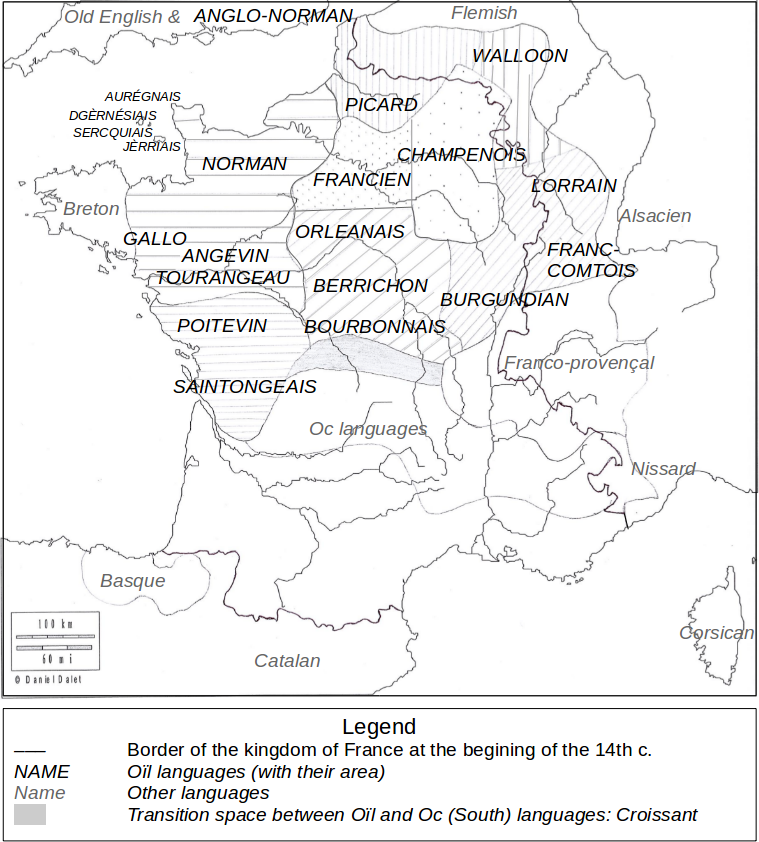
\includegraphics[scale=0.29]{static/media/mod_eval/bertrade/map-dialects2.png}
    \caption{Oïl languages}
    \label{fig:map-dialects}
\end{figure}

There are also many cases of syntactic ambiguity. For example, in the following quote from \emph{Lancelot},\footnote{In the edition from Pierre Kunstmann, from the online \textit{Base de français médiéval}: \url{http://catalog.bfm-corpus.org/CharretteKu}.} (verse ~5436),
both \enquote{la dame} and \enquote{Lancelot} could be the subject or the object of \enquote{Vit} and only the context enables the reader to understand that \enquote{la dame} is the subject.

    \digloss{Dolant et pansif Lancelot Vit la dame}
    {Mournful and meditative Lancelot saw the lady}
    {The lady saw that Lancelot was mournful and meditative.}

Word order is also relatively free within constituents. For example, a noun modifier can be on the left or on the right of its governor, and it is not necessarily preceded by a preposition. In contemporary French, it can only appear on the right, and it is found without a preposition only in some cases like named entities. Because of the general free word order and the absence of punctuation in our treebank, this adds up to the ambiguity of the analysis.

In each of the following examples from the SRCMF corpus, the noun following \emph{roi} (\enquote{king}) has a different analysis: head of \emph{roi}, modifier, argument of the same verb or a different one, with no explicit marking:

\begin{center}
    % beroul. modifieur à gauche.
    \begin{dependency}[theme=simple]
        \begin{deptext}[row 2/.style={font=\small}]
            \textit{Fus} \& \textit{tu} \& \textit{donc} \& \textit{pus} \& \textit{a} \& \textit{la} \& \textbf{\textit{roi}} \& \textit{cort} \\
            %VERB \& PRON \& ADV \& ADV \& ADP \& DET \& NOUN \& NOUN \\
            Were \& you \& then \& no more \& at \& the \& king \& court \\
        \end{deptext}
        \depedge{8}{7}{nmod}
        \depedge[edge start x offset=0.5em]{8}{6}{det}
        \depedge[edge start x offset=1em]{8}{5}{case}
    \end{dependency}

    \raggedright
    \enquote{Then were you not at the king's court anymore?} (\emph{Beroul Tristan})
\end{center}

\begin{center}
    % Graal. modifieur à droite.
    \begin{dependency}[theme=simple]
        \begin{deptext}[row 2/.style={font=\small}]
            \textit{la} \& \textit{fille} \& \textit{au} \& \textit{riche} \& \textbf{\textit{roi}} \& \textit{pescheor} \\
            the \& daughter \& of the \& rich \& king \& fisher \\
        \end{deptext}
        \depedge{5}{6}{flat}
    \end{dependency}

    \raggedright
    \enquote{the daughter of the rich Fisher King} (\emph{Queste del Saint Graal})
\end{center}

\begin{center}
    % Roland. arguments du même verbe.
    \begin{dependency}[theme=simple]
        \begin{deptext}[row 2/.style={font=\small}]
            \textit{De} \& \textit{Guenelun} \& \textit{atent} \& \textit{li} \& \textbf{\textit{reis}} \& \textit{nuveles} \\
            From \& Ganelon \& waits \& the \& king \& news \\
        \end{deptext}
        \depedge{3}{5}{nsubj}
        \depedge[edge start x offset=-0.5em]{3}{6}{obj}
    \end{dependency}

    \raggedright
    \enquote{The king waits for news from Ganelon.} (\emph{Chanson de Roland})
\end{center}

\begin{center}
    % Graal. arguments de verbes différents, et absence de ponctuation.
    \begin{dependency}[theme=simple]
        \begin{deptext}[row 2/.style={font=\small}]
            \textit{Biax} \& \textit{sire} \& \textit{fet} \& \textit{li} \& \textbf{\textit{rois}} \& \textit{escu} \& \textit{vos} \& \textit{envoiera} \& \textit{Diex} \\
            Dear \& Sir \& says \& the \& king \& shield \& you \& send-FUT \& God \\
        \end{deptext}
        \depedge{3}{5}{nsubj}
        \depedge{8}{6}{obj}
    \end{dependency}

    \raggedright
    \enquote{Dear Sir, says the king, God will send you a shield.} (\emph{Queste del Saint Graal})
\end{center}

Furthermore, overt subjects are not mandatory, and are often dropped in texts written in verse until the 12th century, after which the presence of subjects increases through time.
These phenomena are particularly prevalent in verse, where metric and rhyming constraints often lead to more contrived syntactic forms than in prose.

Another source of ambiguity is the variety of spellings, due to the lack of spelling standard. For example, the word \textit{moult} (transl. \textit{a lot (of), very}), emblematic of this period, is initially an adjective, and it is progressively grammaticalized, becoming an adverb. Several forms appear at the same time, some with a declension, some without, and the radical does not have a fixed spelling: \textit{molt(e)(s), molz, mult(e)(s), mul(t)z, mou(l)t}…

\subsection{Early Modern French}\label{def:early}

\begin{table}[!htp]
    \centering\small
    \begin{tabular}{@{}p{0.3\linewidth}p{0.3\linewidth}p{0.3\linewidth}@{}}
        \toprule
        Source                                                                                                                                                                                                                                                                                               & Normalized & Translation \\
        \midrule
        Surquoy, SIRE, s’il plaiſt à voſtre Maieſté de ſe ſouuenir des miſeres de ſon Eſtat, dõt au moins ell’a tiré cét aduantage, qu’en vne grande ieuneſse ell’a acquis vne grande experi\~ece, elle verra que tous les mal-heurs de sõ bas âge ont pris leur commencement en ſemblables occaſions;       &
        \emph{Sur quoi, SIRE, s’il plaît à votre Majesté de se souvenir des misères de son état dont au moins elle a tiré cet avantage, qu’en une grande jeunesse elle a acquis une grande expérience, elle verra que tous les malheurs de son bas âge ont pris leur commencement en semblables occasions~;} &
        \textcolor{gray}{``Whereupon, SIR, if it pleases your Majesty to remember the miseries of her state, from which at least she has derived this advantage, that in great youth she has acquired great experience, she will see that all the misfortunes of her early life took their beginning on similar occasions;''}           \\
        \bottomrule
    \end{tabular}
    \caption{\label{tab:norm_examples}Example of normalization taken from the \emph{Lettres} of \protect\newcite{balzac-1624-lettres}.}
\end{table}

We loosely define Early Modern French as a state of language following Middle French in 1500---following here the \emph{terminus ad quem} used by the \emph{Dictionnaire de Moyen Français} \cite{martin-2020-dictionnaire}---and ending with the French Revolution in 1789. It therefore encompasses three centuries (16\textsuperscript{th}, 17\textsuperscript{th} and 18\textsuperscript{th}\,c.), or two linguistic periods: the \emph{français préclassique} or ``preclassical French'', 1500--1630 and the \emph{français classique} or ``classical French'', 1630--1689; both periodizations are currently used in French linguistics (\emph{e.g.}~by \newcite{vachon-2010-changement} and \newcite{amatuzzi-etal-2019-ameliorer}).

A typical example of Early Modern French, taken from ~\newcite{balzac-1624-lettres}, is given in Table~\ref{tab:norm_examples}. We note here the presence of several phenomena that have now disappeared in contemporary French, such as the presence of abbreviations (\emph{dõt}$\to$\emph{dont}), the long \emph{s} (\emph{ſ}, see\,\emph{miſeres}), the use of \emph{v} instead of \emph{u} (\emph{vne} for \emph{une}), the conservation of etymological letters (\emph{voſtre}$<$Latin~\emph{vŏster} rather than \emph{votre}) and calligraphic letters (\emph{-y} in \emph{Surquoy}), the absence of welding  (\emph{\mbox{mal-heurs}} and not \emph{malheurs}) and the opposite (\emph{Surquoy} and not \emph{Sur quoi}).

For NLP tasks, which process raw sequences, such differences with respect to contemporary French are not trivial, and they prevent the processing of historical texts with tools trained on recent sources.

\section{Outline}



%SOTA
%%%%%%%%%%%%%%%%%%%%%%%%%%%%%%%%%%%%%%%%%%%%%%%%%%%%%%%%%%%%%%%%%%%%%%%%
\chapter{Goclassy Related Work}
%%%%%%%%%%%%%%%%%%%%%%%%%%%%%%%%%%%%%%%%%%%%%%%%%%%%%%%%%%%%%%%%%%%%%%%%

\section{Related Work}

Common Crawl has already been successfully used to train language models, even multilingual ones. The most notable example in probably fastText which was first trained for English using Common Crawl \citep{mikolov-etal-2018-advances} and then for other 157 different languages \citep{grave-etal-2018-learning}. In fact \citet{grave-etal-2018-learning} proposed a pipeline to filter, clean and classify Common Crawl, which we shall call the ``fastText pre-processing pipeline.'' They used the fastText linear classifier \citep{joulin-etal-2016-fasttext, joulin-etal-2017-bag} to classify each line of Common Crawl by language, and downloaded the initial corpus and schedule the I/O using some simple Bash scripts. Their solution, however, proved to be a synchronous blocking pipeline that works well on infrastructures having the necessary hardware to assure high I/O speeds even when storing tens of terabytes of data at a time. But that downscales poorly to medium-low resource infrastructures that rely on more traditional cost-effective electromechanical mediums in order to store this amount of data.

Concerning contextual models, \citet{baevski-etal-2019-cloze} trained a BERT-like bi-directional Transformer for English using Common Crawl. They followed the ``fastText pre-processing pipeline'' but they removed all copies of Wikipedia inside Common Crawl. They also trained their model using News Crawl \citep{bojar-etal-2018-findings} and using Wikipedia~+~BooksCorpus, they compared three models and showed that Common Crawl gives the best performance out of the three corpora.

The XLNet model was trained for English by joining the BookCorpus, English Wikipedia, Giga5 \citep{parker-etal-2011-english}, ClueWeb 2012-B \citep{callan-etal-2009-clueweb09} and Common Crawl. Particularly for Common Crawl, \citet{yang-etal-2019-xlnet} say they use ``heuristics to aggressively filter out short or low-quality articles'' from Common Crawl, however they don't give any detail about these ``heuristics'' nor about the pipeline they use to classify and extract the English part of Common Crawl.

It is important to note that none of these projects distributed their classified, filtered and cleaned versions of Common Crawl, making it difficult in general to faithfully reproduce their results.

\section{Common Crawl}

Common Crawl is a non-profit foundation which produces and maintains an open repository of web crawled data that is both accessible and analysable.\footnote{\url{http://commoncrawl.org/about/}} Common Crawl's complete web archive consists of petabytes of data collected over 8 years of web crawling. The repository contains raw web page HTML data (WARC files), metdata extracts (WAT files) and plain text extracts (WET files). The organisation's crawlers has always respected \texttt{nofollow}\footnote{\url{http://microformats.org/wiki/rel-nofollow}} and \texttt{robots.txt}\footnote{\url{https://www.robotstxt.org/}} policies.

Each monthly Common Crawl snapshot is in itself a massive multilingual corpus, where every single file contains data coming from multiple web pages written in a large variety of languages and covering all possible types of topics. Thus, in order to effectively use this corpus for the previously mentioned Natural Language Processing and Machine Learning applications, one has first to extract, filter, clean and classify the data in the snapshot by language.

For our purposes we use the WET files which contain the extracted plain texts from the websites mostly converted to UTF-8, as well as headers containing the metatada of each crawled document. Each WET file comes compressed in gzip format\footnote{\url{https://www.gnu.org/software/gzip/}} and is stored on Amazon Web Services. We use the November 2018 snapshot which surpasses 20TB of uncompressed data and contains more than 50 thousand plain text files where each file consists of the plain text from multiple websites along its metadata header. From now on, when we mention the ``Common Crawl'' corpus, we refer to this particular November 2018 snapshot.

\section{fastText's Pipeline}

In order to download, extract, filter, clean and classify Common Crawl we base ourselves on the ``fastText pre-processing pipeline'' used by \citet{grave-etal-2018-learning}. Their pipeline first launches multiple process, preferably as many as available cores. Each of these processes first downloads one Common Crawl WET file which then proceeds to decompress after the download is over. After decompressing, an instance of the fastText linear classifier \citep{joulin-etal-2016-fasttext, joulin-etal-2017-bag} is launched, the classifier processes each WET file line by line, generating a language tag for each line. The tags are then stored in a tag file which holds a one-to-one correspondence between lines of the WET file and its corresponding language tag. The WET file and the tag files are read sequentially and each on the WET file line holding the condition of being longer that 100 bytes is appended to a language file containing only plain text (tags are discarded). Finally the tag file and the WET files are deleted.

Only when one of these processes finishes another can be launched. This means that one can at most process and download as many files as cores the machine has. That is, if for example a machine has 24 cores, only 24 WET files can be downloaded and processed simultaneously, moreover, the 25\textsuperscript{th} file won't be downloaded until one of the previous 24 files is completely processed.

When all the WET files are classified, one would normally get around 160 language files, each file holding just plain text written in its corresponding language. These files still need to be filtered in order to get rid of all files containing invalid UTF-8 characters, so again a number of processes are launched, this time depending on the amount of memory of the machine. Each process reads a language file, first filters for invalid UTF-8 characters and then performs deduplication. A simple non-collision resistant hashing algorithm is used to deduplicate the files.

The fastText linear classifier works by representing sentences for classification as Bags of Words (BoW) and training a linear classifier. A weight matrix $A$ is used as a look-up table over the words and the word representations are then averaged into a text representation which is fed to the linear classifier. The architecture is in general similar to the CBoW model of \citet{mikolov-etal-2013-distributed} but the middle word is replaced by a label. They uses a softmax function $f$ to compute the probability distribution over the classes. For a set of $N$ documents, the model is trained to minimise the negative log-likelihood over the classes:
\[
    -\frac{1}{N}\sum_{n=1}^{N} y_n\log\left(f(BAx_n)\right),
\]
where $x_n$ is the normalised bag of features of the $n$-th document, $y_n$ is the $n$-th label, and $A,B$ are the weight matrices. The pre-trained fastText model for language recognition \citep{grave-etal-2018-learning} is capable of recognising around 176 different languages and was trained using 400 million tokens from Wikipedia as well as sentences from the Tatoeba website\footnote{\url{https://tatoeba.org/}}.

%%%%%%%%%%%%%%%%%%%%%%%%%%%%%%%%%%%%%%%%%%%%%%%%%%%%%%%%%%%%%%%%%%%%%%%%
\chapter{Monolingual Related Work}
%%%%%%%%%%%%%%%%%%%%%%%%%%%%%%%%%%%%%%%%%%%%%%%%%%%%%%%%%%%%%%%%%%%%%%%%

Since the introduction of \emph{word2vec} \citep{mikolov-etal-2013-distributed}, many attempts have been made to create multilingual language representations; for fixed word embeddings the most remarkable works are those of \citep{al-rfou-etal-2013-polyglot} and \citep{bojanowski-etal-2017-enriching} who created word embeddings for a large quantity of languages using Wikipedia, and later \citep{grave-etal-2018-learning} who trained the fastText word embeddings for 157 languages using Common Crawl and who in fact showed that using crawled data significantly increased the performance of the embeddings especially for mid- to low-resource languages.

Regarding contextualized models, the most notable non-English contribution has been that of the mBERT \citep{devlin-etal-2019-bert}, which is distributed as (i)~a single multilingual model for 100 different languages trained on Wikipedia data, and as (ii)~a single multilingual model for both Simplified and Traditional Chinese. Four monolingual fully trained ELMo models have been distributed for Japanese, Portuguese, German and Basque\footnote{\url{https://allennlp.org/elmo}}; 44 monolingual ELMo models\footnote{\url{https://github.com/HIT-SCIR/ELMoForManyLangs}} where also released by the \emph{HIT-SCIR} team \citep{che-etal-2018-towards} during the \emph{CoNLL 2018 Shared Task} \citep{zeman-etal-2018-conll}, but their training sets where capped at 20 million words. A German BERT \citep{chan-etal-2019-german} as well as a French BERT model (called CamemBERT) \citep{martin-etal-2020-camembert} have also been released. In general no particular effort in creating a set of high-quality monolingual contextualized representations has been shown yet, or at least not on a scale that is comparable with what was done for fixed word embeddings.

For dependency parsing and POS tagging the most notable non-English specific contribution is that of the \emph{CoNLL 2018 Shared Task} \citep{zeman-etal-2018-conll}, where the 1\textsuperscript{st} place (LAS Ranking) was awarded to the \emph{HIT-SCIR} team \citep{che-etal-2018-towards} who used \citet{dozat-manning-2017-deep}'s \emph{Deep Bi-affine parser} and its extension described in \citep{dozat-etal-2017-stanfords}, coupled with deep contextualized ELMo embeddings \citep{peters-etal-2018-deep} (capping the training set at 20 million words). The 1\textsuperscript{st} place in universal POS tagging was awarded to \citet{smith-etal-2018-82} who used two separate instances of \citet{bohnet-etal-2018-morphosyntactic}'s tagger.

More recent developments in POS tagging and parsing include those of \citet{straka-strakova-2019-evaluating} which couples another CoNLL 2018 shared task participant, UDPipe 2.0 \citep{straka-2018-udpipe}, with mBERT greatly improving the scores of the original model, and UDify \citep{kondratyuk-straka-2019-75}, which adds an extra attention layer on top of mBERT plus a Deep Bi-affine attention layer for dependency parsing and a Softmax layer for POS tagging. UDify is actually trained by concatenating the training sets of 124 different UD treebanks, creating a single POS tagging and dependency parsing model that works across 75 different languages.

%%%%%%%%%%%%%%%%%%%%%%%%%%%%%%%%%%%%%%%%%%%%%%%%%%%%%%%%%%%%%%%%%%%%%%%%
\chapter{Quality at Glance Related Work}
%%%%%%%%%%%%%%%%%%%%%%%%%%%%%%%%%%%%%%%%%%%%%%%%%%%%%%%%%%%%%%%%%%%%%%%%

\section{Related Work}\label{sec:related}

Corpora collected by web crawlers are known to be noisy~\citep{junczys-dowmunt-2019-microsoft,luccioni-viviano-2021-whats}. In highly multilingual settings, past work found that web-crawls of lower-resource languages have serious issues, especially with segment-level LangID~\citep{caswell-etal-2020-language}.
%Repeated studies have shown that 
Cleaning and filtering web-crawls can boost general language modeling~\citep{gao-etal-2020-the,brown-etal-2020-language,raffel-etal-2020-exploring} and downstream task performance~\citep{moore-lewis-2010-intelligent,rarrick-etal-2011-mt,xu-koehn-2017-zipporah,khayrallah-koehn-2018-impact,brown-etal-2020-language}.

As the scale of ML research grows, it becomes increasingly difficult to validate automatically collected and curated datasets \citep{biderman-etal-2020-pitfalls,birhane-etal-2021-large,bender-etal-2021-on}.
%Data Quality Considerations for Big Data and Machine Learning: Going Beyond Data Cleaning and Transformations \citep{gudivada2017data}
Several works have focused on advancing methodologies and best practices to address these challenges. \citet{bender-friedman-2018-data} introduced data statements, a documentary framework for NLP datasets that seeks to provide a universal minimum bar for dataset description. Similar work has been done on systematizing documentation in other areas in data science and machine learning, including work focusing on
online news \citep{kevin-etal-2018-information}, data ethics \citep{sun-etal-2019-mithralabel}, and data exploration \citep{holland-etal-2018-the}, as well as generalist work such as \citep{gebru-etal-2018-datasheets}. 
Data quality is also implicitly documented by successes of filtering methods. There is a large literature on filtering data for various NLP tasks, e.g. \citet{axelrod-etal-2011-domain,moore-lewis-2010-intelligent,rarrick-etal-2011-mt,wang-etal-2018-denoising,kamholz-etal-2014-panlex,junczys-dowmunt-2018-dual,caswell-etal-2020-language}.

Closest to our work is the analysis of a highly multilingual (non-publicly available) web-crawl and LangID related quality issues by \citet{caswell-etal-2020-language}.
%, performing a highly multilingual web-crawl and then systematically analyzing the LangID related quality issues. 
%However, though 
They perform a brief analysis of the quality of OSCAR
%, but omit analyses of any other public datasets, 
with the focus only on the presence of in-language content.
\citet{dodge-etal-2021-documenting} automatically documented and analyzed the contents and sources of C4~\citep{raffel-etal-2020-exploring}, the English counterpart of mC4, which surfaced the presence of machine-translated contents and NLP benchmark data.

\section{Multilingual Corpora}\label{sec:crawls}

\begin{table*}[th!]
    \centering
    \resizebox{\textwidth}{!}{%
        \begin{tabular}{lccccc}
            \toprule
                            & \multicolumn{3}{c}{\textbf{Parallel}} & \multicolumn{2}{c}{\textbf{Monolingual}}                                                       \\
            \cmidrule(lr){2-4} \cmidrule(lr){5-6}
                            & \textbf{CCAligned}                    & \textbf{ParaCrawl v7.1}                  & \textbf{WikiMatrix} & \textbf{OSCAR} & \textbf{mC4} \\
            \midrule
            \#languages     & 137                                   & 41                                       & 85                  & 166            & 101          \\
            Source          & CC 2013--2020                         & selected websites                        & Wikipedia           & CC 11/2018     & CC all       \\
            Filtering level & document                              & sentence                                 & sentence            & document       & document     \\
            Langid          & FastText                              & CLD2                                     & FastText            & FastText       & CLD3         \\
            Alignment       & LASER                                 & Vec/Hun/BLEU-Align                       & LASER               & -              & -            \\
            Evaluation      & TED-6                                 & WMT-5                                    & TED-45              & POS/DEP-5      & XTREME       \\
            \bottomrule
        \end{tabular}%
    }
    \caption{Comparison of parallel and monolingual corpora extracted from web documents, including their downstream evaluation tasks. All parallel corpora are evaluated for machine translation (BLEU). TED-6: \texttt{da}, \texttt{cr}, \texttt{sl}, \texttt{sk}, \texttt{lt}, \texttt{et}; TED-45: 45-language subset of ~\citep{qi-etal-2018-pre}; WMT-5: \texttt{cs}, \texttt{de}, \texttt{fi}, \texttt{lv}, \texttt{ro}. POS/DEP-5: part-of-speech labeling and dependency parsing for \texttt{bg}, \texttt{ca}, \texttt{da}, \texttt{fi}, \texttt{id}.}
    \label{tab:corpora}
\end{table*}
% CC: CommonCrawl; TED-6: da, cr, sl, sk, lt, et; TED-50: TODO cite Qi et al. 2018; WMT-5: cs, de, fi, lv, ro.
%fastText: 176 languages, Wikipedia & Tatoeba


Table \ref{tab:corpora} provides an overview of the corpora of interest in this work. We selected the corpora for their multilinguality and the inclusion of understudied languages in NLP. With the exception of WikiMatrix and ParaCrawl, all corpora are derived from CommonCrawl (CC).\footnote{\url{http://commoncrawl.org/}} %s, and distinguish themselves by the choice of filtering methods, LangID and automatic alignment technology.
%LangID is crucial to corpus creation, since any issues within might propagate, e.g. bias recognizing document types similar to what it was trained on, or errors in language identifiers.\footnote{\url{https://github.com/facebookresearch/fastText/issues/482}}


\paragraph{CCAligned~\citep{el-kishky-etal-2020-ccaligned}}is a %119-language\footnote{119 of originally 137 available for download (02/2021)}
%Although 137 language pairs are reported in ~\citet{el-kishky-etal-2020-ccaligned}, only 119 sentence-level corpora were available to download on \url{statmt.org} as of February 2021.}
parallel dataset built off 68 CC snapshots. Documents are aligned if they are in the same language according to FastText LangID~\citep{joulin-etal-2016-fasttext,joulin-etal-2017-bag}, and have the same URL but for a differing language code. These alignments are refined with cross-lingual LASER embeddings \citep{artetxe-schwenk-2019-massively}. For sentence-level data, they split on newlines and align with LASER, but perform no further filtering.
Human annotators evaluated the quality of document alignments for six languages (\texttt{de}, \texttt{zh}, \texttt{ar}, \texttt{ro}, \texttt{et}, \texttt{my}) selected for their different scripts and amount of retrieved documents, reporting precision of over 90\%.
% Latin, Chinese, Arabic, Burmese script
The quality of the extracted parallel sentences was evaluated in a machine translation (MT) task on six European (\texttt{da}, \texttt{cr}, \texttt{sl}, \texttt{sk}, \texttt{lt}, \texttt{et}) languages of the TED corpus~\citep{qi-etal-2018-pre}, where it compared favorably to systems built on crawled sentences from WikiMatrix and ParaCrawl v6. %, yielding BLEU scores in a range between 15 and 38.  

\paragraph{Multilingual C4 (mC4)~\citep{xue-etal-2021-mt5}} is a document-level dataset used for training the mT5 language model. It consists of monolingual text in 101 languages and is generated from 71 CC snapshots. It filters out pages that contain less than three lines of at least 200 characters and pages that contain bad words.\footnote{\url{https://github.com/LDNOOBW/}} Since this is a document-level dataset, we split it by sentence and deduplicate it before rating. For language identification, it uses CLD3~\citep{botha-etal-2017-natural},\footnote{\url{https://github.com/google/cld3/}} a small feed-forward neural network that was trained to detect 107 languages.
The mT5 model pre-trained on mC4
is evaluated on 6 tasks of the XTREME benchmark~\citep{hu-etal-2020-xtreme} covering a variety of languages and outperforms other multilingual pre-trained language models such as mBERT~\citep{devlin-etal-2019-bert} and XLM\nobreakdash-R~\citep{conneau-etal-2020-unsupervised}.%\footnote{mBERT is trained on Wikipedia, {XML\nobreakdash-R} on CommonCrawl.} 

\paragraph{OSCAR~\citep{ortiz-suarez-etal-2019-asynchronous, ortiz-suarez-etal-2020-monolingual}}is a set of monolingual corpora extracted from CC snapshots, specifically from the plain text \emph{WET} format distributed by CC which removes all the HTML tags and converts the text to UTF-8. It is deduplicated and follows the approach by~\citep{grave-etal-2018-learning} of using FastText LangID~\citep{joulin-etal-2016-fasttext, joulin-etal-2017-bag} on a line-level.\footnote{\url{https://fasttext.cc/docs/en/language-identification.html} } No other filtering was applied.
% 
For five languages (\texttt{bg}, \texttt{ca}, \texttt{da}, \texttt{fi}, \texttt{id}) OSCAR was used by its original authors to train language models which were then evaluated on parsing and POS tagging \citep{ortiz-suarez-etal-2020-monolingual}. OSCAR has also been used in independent studies to train monolingual or multilingual language models (\texttt{ar}, \texttt{as}, \texttt{bn}, \texttt{de}, \texttt{el}, \texttt{fr}, \texttt{gu}, \texttt{he}, \texttt{hi}, \texttt{kn}, \texttt{ml}, \texttt{mr}, \texttt{nl}, \texttt{or}, \texttt{pa}, \texttt{ro}, \texttt{ta}, \texttt{te}) and subsequently evaluate them on various downstream tasks \citep{antoun-etal-2021-araelectra, kakwani-etal-2020-indicnlpsuite, wilie-etal-2020-indonlu, chan-etal-2020-germans, koutsikakis-etal-2020-greek, martin-etal-2020-camembert, chriqui-etal-2021-hebert, seker-etal-2021-alephbert, delobelle-etal-2020-robbert, dumitrescu-etal-2020-birth, masala-etal-2020-robert}.


\paragraph{ParaCrawl v7.1} is a parallel dataset with 41 language pairs primarily aligned with English (39 out of 41) and mined using the parallel-data-crawling tool Bitextor \citep{espla-etal-2019-paracrawl,banon-etal-2020-paracrawl} which includes downloading documents, preprocessing and normalization, aligning documents and segments, and filtering noisy data via Bicleaner.\footnote{\url{https://github.com/bitextor/bicleaner}}
ParaCrawl focuses on European languages, but also includes 9 lower-resource, non-European language pairs in v7.1.
% TODO: https://www.aclweb.org/anthology/2020.eamt-1.31.pdf \citep{ramirez-sanchez-etal-2020-bifixer}
Sentence alignment and sentence pair filtering choices were optimized for five languages (\texttt{mt}, \texttt{et}, \texttt{hu}, \texttt{cs}, \texttt{de}) by training and evaluating MT models on the resulting parallel sentences. An earlier version (v5) was shown to improve translation quality on WMT benchmarks for~\texttt{cs}, \texttt{de}, \texttt{fi}, \texttt{lv}, \texttt{ro}.


\paragraph{WikiMatrix~\citep{schwenk-etal-2021-wikimatrix}} is a public dataset containing 135M parallel sentences in 1620 language pairs (85 languages) mined from Wikipedia. Out of the 135M parallel sentences, 34M are aligned with English. %, which we focus on.
%which relies on first learning multilingual sentence embeddings, and then applying the cosine distance metric to determine whether two sentences are close enough to be considered translations of each other.
The text is extracted from Wikipedia pages, split into sentences, and duplicate sentences are removed. FastText LangID is used before identifying bitext with LASER's distance-based mining approach.
The margin threshold is optimized by training and evaluating downstream MT models on four WMT benchmarks (\texttt{de-en}, \texttt{de-fr}, \texttt{cs-de}, \texttt{cs-fr}). The final dataset is used to train translation models that are then evaluated by automatically measuring the quality of their translations against human translations of TED talks in 45 languages, with highest quality for translations between English and e.g. \texttt{pt}, \texttt{es}, \texttt{da}, and lowest for \texttt{sr}, \texttt{ja}, \texttt{mr}, \texttt{zh\_TW}.
In the audit we focus on language pairs with English on one side.
% https://github.com/facebookresearch/LASER/blob/master/tasks/WikiMatrix/WikiMatrix-bleu.pdf

%%%%%%%%%%%%%%%%%%%%%%%%%%%%%%%%%%%%%%%%%%%%%%%%%%%%%%%%%%%%%%%%%%%%%%%%
\chapter{Towards Related Work}
%%%%%%%%%%%%%%%%%%%%%%%%%%%%%%%%%%%%%%%%%%%%%%%%%%%%%%%%%%%%%%%%%%%%%%%%

Crawled data and more specifically Common Crawl\footnote{\url{https://commoncrawl.org}} has been extensively used for pre-training language representations and large generative language models in recent years. One of the first proposed pipelines to automatically classify Common Crawl by language was that of \newcite{grave-etal-2018-learning}, it classified Common Crawl entries at line level using the FastText linear classifier \cite{joulin-etal-2016-fasttext,joulin-etal-2017-bag}. However, even though FastText word embeddings were released for 157 different languages \cite{grave-etal-2018-learning}, the data itself was never released.

Later \newcite{ortiz-suarez-etal-2019-asynchronous} reproduced and optimized \newcite{grave-etal-2018-learning} pipeline and actually released the data which came to be the first version of the OSCAR corpus (now referred to as OSCAR 2019). This pipeline was then rewritten and optimized by \newcite{abadji-etal-2021-ungoliant} which in turn released a second version of OSCAR (referred to as OSCAR 21.09) but, other than adding the metadata and using a more recent dump of Common Crawl, it remained virtually the same as the original one proposed by \newcite{ortiz-suarez-etal-2019-asynchronous}. All these three mentioned pipelines \cite{grave-etal-2018-learning,ortiz-suarez-etal-2019-asynchronous,abadji-etal-2021-ungoliant} classified Common Crawl's text at the line level, meaning that the apparent \emph{``documents''} of OSCAR were actually just contiguous lines of text that were classified as being the same language. This approach preserved somehow the document integrity of monolingual entries in Common Crawl, but it completely destroyed the document integrity of multilingual entries.

Parallel to the development of OSCAR, there is also Multilingual C4 (mC4) \cite{xue-etal-2021-mt5} and CCNet \cite{wenzek-etal-2020-ccnet} both of which are also derived from Common Crawl but propose pipelines that propose a document level language classification as opposed to OSCAR's line level classification. Both CCNet and mC4 pipelines proposed methods for filtering \emph{``undesired''} data: CCNet used small language models trained on Wikipedia and based on the KenLM library \cite{heafield-2011-kenlm} while mC4 used a simple badword filter\footnote{\url{https://github.com/LDNOOBW/}}.

%%%%%%%%%%%%%%%%%%%%%%%%%%%%%%%%%%%%%%%%%%%%%%%%%%%%%%%%%%%%%%%%%%%%%%%%
\chapter{CamemBERT Related Work}
%%%%%%%%%%%%%%%%%%%%%%%%%%%%%%%%%%%%%%%%%%%%%%%%%%%%%%%%%%%%%%%%%%%%%%%%

\section{Previous work}
\label{relatedwork}
\subsection{Contextual Language Models}
\paragraph{From non-contextual to contextual word embeddings}
The first neural word vector representations were non-contextualized word embeddings, most notably
word2vec \citep{mikolov-etal-2013-distributed}, GloVe \cite{pennington-etal-2014-glove} and fastText \cite{mikolov-etal-2018-advances}, which were designed to be used as input to task-specific neural architectures.
Contextualized word representations such as ELMo \cite{peters-etal-2018-deep} and flair \cite{akbik-etal-2018-contextual}, improved the representational power of word embeddings by taking context into account. Among other reasons, they improved the performance of models on many tasks by handling words polysemy.
This paved the way for larger contextualized models that replaced downstream architectures altogether in most tasks. Trained with language modeling objectives, these approaches range from LSTM-based architectures such as \cite{dai-le-2015-semi}, to the successful transformer-based architectures such
as GPT2 \cite{radford-etal-2019-language}, \bert \cite{devlin-etal-2019-bert}, \roberta \cite{liu-etal-2019-roberta} and more recently ALBERT \cite{lan-etal-2020-albert} and T5 \cite{raffel-etal-2020-exploring}.


\paragraph{Non-English contextualized models}
\label{contextualmodelsforotherlanguages}
Following the success of large pretrained language models, they were extended to the multilingual setting with multilingual \bert (hereafter \mbert) \cite{devlin-etal-2019-bert}, a single multilingual model for 104 different languages trained on Wikipedia data, and later XLM \cite{conneau-lample-2019-cross}, which significantly improved unsupervized machine translation.
More recently XLM-R \cite{conneau-etal-2020-unsupervised}, extended XLM by training on 2.5TB of data and outperformed previous scores on multilingual benchmarks. They show that multilingual models can obtain results competitive with monolingual models by leveraging higher quality data from other languages on specific downstream tasks.

A few non-English monolingual models have been released: ELMo models for Japanese, Portuguese, German and Basque\footnote{\url{https://allennlp.org/elmo}} and BERT for Simplified and Traditional Chinese \cite{devlin-etal-2019-bert} and German \cite{chan-etal-2019-german}.

However, to the best of our knowledge, no particular effort has been made toward training models for languages other than English at a scale similar to the latest English models (e.g.~\roberta trained on more than 100GB of data).

\paragraph{BERT and RoBERTa}
Our approach is based on \roberta \cite{liu-etal-2019-roberta} which itself is based on \bert \cite{devlin-etal-2019-bert}.
\bert is a multi-layer bidirectional Transformer encoder trained with a masked language modeling (MLM) objective, inspired by the Cloze task \cite{taylor-1953-cloze}.
It comes in two sizes: the \bertbase architecture and the \bertlarge architecture. The \bertbase architecture is 3 times smaller and therefore faster and easier to use while \bertlarge achieves increased performance on downstream tasks.
\roberta improves the original implementation of \bert by identifying key design choices for better performance, using dynamic masking, removing the next sentence prediction task, training with larger batches, on more data, and for longer.


\section{Downstream evaluation tasks}

In this section, we present the four downstream tasks that we use to evaluate \camembert, namely: Part-Of-Speech (POS) tagging, dependency parsing, Named Entity Recognition (NER) and Natural Language Inference (NLI). We also present the baselines that we will use for comparison.

%\lm{Merge all tasks together}
%\subsection{Part-of-speech tagging and dependency parsing}\label{subsection:pos_and_dp}

\paragraph{Tasks} POS tagging is a low-level syntactic task, which consists in assigning to each word its corresponding grammatical category. Dependency parsing consists in predicting the labeled syntactic tree in order to capture the syntactic relations between words.

For both of these tasks we run our experiments using the Universal Dependencies (UD)\footnote{\url{https://universaldependencies.org}} framework and its corresponding UD POS tag set \citep{petrov-etal-2012-universal} and UD treebank collection \citep{nivre-etal-2018-universal}, which was used for the CoNLL 2018 shared task \citep{seker-etal-2018-universal}. We perform our evaluations on the four freely available French UD treebanks in UD~v2.2: GSD \citep{mcdonald-etal-2013-universal}, Sequoia\footnote{\url{https://deep-sequoia.inria.fr}} \citep{candito-seddah-2012-le,candito-etal-2014-deep}, Spoken \citep{lacheret-etal-2014-rhapsodie,bawden-etal-2014-correcting}\footnote{Speech transcript uncased that includes annotated disfluencies without punctuation}, and ParTUT \cite{sanguinetti-Bosco-2015-parttut}. A brief overview of the size and content of each treebank can be found in Table \ref{treebanks-tab}.

\begin{table}[ht]
    \centering\small
        \begin{tabular}{lccl}
            \toprule
            Treebank                         & \#Tokens                         & \#Sentences                     & \multicolumn{1}{l}{Genres} \\
            \midrule
                                             &                                  &                                 & Blogs, News                \\
            \multirow{-2}{*}[1.5pt]{GSD}     & \multirow{-2}{*}[1.5pt]{389,363} & \multirow{-2}{*}[1.5pt]{16,342} & Reviews, Wiki              \\ \tabucline[\hbox {$\scriptstyle \cdot$}]{-}
                                             &                                  &                                 & Medical, News              \\
            \multirow{-2}{*}[0.7pt]{Sequoia} & \multirow{-2}{*}[0.7pt]{68,615}  & \multirow{-2}{*}[0.7pt]{3,099}  & Non-fiction, Wiki          \\ \tabucline[\hbox {$\scriptstyle \cdot$}]{-}
            Spoken                           & 34,972                           & 2,786                           & Spoken                     \\ \tabucline[\hbox {$\scriptstyle \cdot$}]{-}
            ParTUT                           & 27,658                           & 1,020                           & Legal, News, Wikis         \\ \tabucline[\hbox {$\scriptstyle \cdot$}]{-}
            FTB                              & 350,930                          & 27,658                          & News                       \\
            \bottomrule
        \end{tabular}
    \caption{Statistics on the treebanks used in POS tagging, dependency parsing, and NER (FTB).}\label{treebanks-tab}
\end{table}

We also evaluate our model in NER, which is a sequence labeling task predicting which words refer to real-world objects, such as people, locations, artifacts and organisations. We use the French Treebank\footnote{This dataset has only been stored and used on Inria's servers after signing the research-only agreement.} (FTB) \citep{abeille-etal-2003-building} in its 2008 version introduced by \citet{candito-crabbe-2009-improving} and with NER annotations by \citet{sagot-etal-2012-annotation}. The FTB contains more than 11 thousand entity mentions distributed among 7 different entity types. A brief overview of the FTB can also be found in Table \ref{treebanks-tab}.

Finally, we evaluate our model on NLI, using the French part of the XNLI dataset \cite{conneau-etal-2018-xnli}. NLI consists in predicting whether a hypothesis sentence is entailed, neutral or contradicts a premise sentence. The XNLI dataset is the extension of the Multi-Genre NLI (MultiNLI) corpus \cite{williams-etal-2018-broad} to 15 languages by translating the validation and test sets manually into each of those languages.
The English training set is machine translated for all languages other than English.
The dataset is composed of 122k train, 2490 development and 5010 test examples for each language.
As usual, NLI performance is evaluated using accuracy.


\paragraph{Baselines}
In dependency parsing and POS-tagging we compare our model with:

\begin{itemize}
    \item \emph{\mbert}: The multilingual cased version of \bert (see Section~\ref{contextualmodelsforotherlanguages}). We fine-tune \mbert on each of the treebanks with an additional layer for POS-tagging and dependency parsing, in the same conditions as our \camembert model.
    \item \emph{\xlmmlmtlm}: A multilingual pretrained language model from \citet{conneau-lample-2019-cross}, which showed better performance than \mbert on NLI. We use the version available in the Hugging's Face transformer library \cite{wolf-etal-2019-huggingface}; like \mbert, we fine-tune it in the same conditions as our model.
    \item \emph{UDify} \cite{kondratyuk-straka-2019-75}: A multitask and multilingual model based on \mbert, UDify is trained simultaneously on 124 different UD treebanks, creating a single POS tagging and dependency parsing model that works across 75 different languages. We report the scores from \citet{kondratyuk-straka-2019-75} paper.
    \item \emph{UDPipe Future} \citep{straka-2018-udpipe}: An LSTM-based model ranked 3\textsuperscript{rd} in dependency parsing and 6\textsuperscript{th} in POS tagging at the CoNLL~2018 shared task \citep{seker-etal-2018-universal}. We report the scores from \citet{kondratyuk-straka-2019-75} paper.
    \item \emph{UDPipe Future + \mbert + Flair} \citep{straka-strakova-2019-evaluating}: The original UDPipe Future implementation using \mbert and Flair as feature-based contextualized word embeddings. We report the scores from \citet{straka-strakova-2019-evaluating} paper.
\end{itemize}

%UDPipe Future+\mbert+Flair settles the state-of-the-art for most UD languages including French for both Universal POS tagging and dependency parsing. Finally, we compare our model to UDPipe Future \cite{straka-2018-udpipe}, a  model ranked 3rd in dependency parsing and 6th in POS tagging during the CoNLL~2018 shared task \cite{seker-etal-2018-universal}. UDPipe Future acts as a strong baseline that does not make use of any pretrained contextual embedding. 

In French, no extensive work has been done on NER due to the limited availability of annotated corpora. Thus we compare our model with the only recent available baselines set by \citet{dupont-2017-exploration}, who trained both CRF \citep{lafferty-etal-2001-conditional} and BiLSTM-CRF \citep{lample-etal-2016-neural} architectures on the FTB and enhanced them using heuristics and pretrained word embeddings. Additionally, as for POS and dependency parsing, we compare our model to a fine-tuned version of \mbert for the NER task.

For XNLI, we provide the scores of \mbert which has been reported for French by \citet{wu-dredze-2019-beto}.
We report scores from \xlmmlmtlm (described above), the best model from \citet{conneau-lample-2019-cross}. %\xlmmlmtlm is smaller than \xlmmultimlm from the same authors (12 layers, hidden size 1024, 8 attention heads, 270M parameters vs.~550M parameters) but authors did not report scores for \xlmmultimlm on XNLI.
We also report the results of \mbox{XLM-R} \cite{conneau-etal-2020-unsupervised}.

%and the English and French Masked Language Model \footnote{we plan to release experiments on XLM-17 and XLM-R} version of XLM referred as \xlmEnFr \cite{conneau-lample-2019-cross}, in order to demonstrate the usefulness of a dedicated version of \bert for French. \xlmEnFr provides us the performance of a multilingual masked language model pretrained on a smaller corpora which is the concatenation of Wikipedia English and French. We finetune those models using the same architecture enhancement and optimization process as we do on \camembert. We then compare our models to UDify \cite{kondratyuk-straka-2019-75} and UDPipe Future+\mbert+Flair \cite{straka-strakova-2019-evaluating}. UDify is a multitask and multilingual model based on \mbert while UDPipe Future+\mbert+Flair is just the original UDPipe Future implementation using \mbert and Flair as contextualized word embeddings. UDify pushed dependency parsing and POS to the extreme case of training one single model based on \mbert for all UD languages reaching state-of-the-art results for many treebanks. 

%Most of the advances in NER have been achieved on English, particularly focusing on the CoNLL 2003 \cite{tjong2003introduction} and the Ontonotes v5 \cite{pradhan2012conll,pradhan2013towards} English corpora. NER is a task that was traditionally tackled using Conditional Random Fields (CRF) \cite{lafferty-etal-2001-conditional} which are quite suited for NER; CRFs were later used as decoding layers for Bi-LSTM architectures \cite{huang2015bidirectional,lample-etal-2016-neural} showing considerable improvements over CRFs alone. These Bi-LSTM-CRF architectures were later enhanced with contextualised word embeddings which yet again brought major improvements to the task \cite{peters-etal-2018-deep,akbik-etal-2018-contextual}. Finally, large pretrained architectures settled the current state of the art showing a small yet important improvement over previous NER-specific architectures \cite{devlin-etal-2019-bert,baevski2019cloze}.

% In non-English NER the CoNLL 2002 shared task included NER corpora for Spanish and Dutch corpora \cite{tjong2002introduction} while the CoNLL 2003 included a German corpus \cite{tjong2003introduction}. Here the recent efforts of \cite{strakova-etal-2019-neural} settled the state of the art for Spanish and Dutch, while \cite{akbik-etal-2018-contextual} did it for German.

%The NER-annotated FTB contains more than 12k sentences and more than 350k tokens extracted from articles of the newspaper \textit{Le Monde} published between 1989 and 1995. In total, it contains 11,636 entity mentions distributed among 7 different types of entities, namely: 2025 mentions of ``Person'', 3761 of ``Location'', 2382 of ``Organisation'', 3357 of ``Company'', 67 of ``Product'', 15 of ``POI'' (Point of Interest) and 29 of ``Fictional Character''. 

%GSD \cite{mcdonald13} is the second-largest treebank available for French after the FTB (described in subsection \ref{ner-section}), it contains data from blogs, news articles, reviews, and Wikipedia. The Sequoia treebank\footnote{\url{https://deep-sequoia.inria.fr}} \cite{candito-seddah-2012-le,candito-etal-2014-deep} contains more than 3000 sentences, from the French Europarl, the regional newspaper \emph{L’Est Républicain}, the French Wikipedia and documents from the European Medicines Agency. Spoken is a corpus converted automatically from the Rhapsodie treebank\footnote{\url{https://www.projet-rhapsodie.fr}} \cite{lacheret-etal-2014-rhapsodie,bawden-etal-2014-correcting} with manual corrections. It consists of 57 sound samples of spoken French with orthographic transcription and phonetic transcription aligned with sound (word boundaries, syllables, and phonemes), syntactic and prosodic annotations. 
%Finally, ParTUT is a conversion of a multilingual parallel treebank developed at the University of Turin, and consisting of a variety of text genres, including talks, legal texts, and Wikipedia articles, among others; ParTUT data is derived from the already-existing parallel treebank Par(allel)TUT \cite{sanguinetti-Bosco-2015-parttut}. Treebanks statistics are summarized in Table~\ref{treebanks-tab}.

%We evaluate the performance of our models using the standard UPOS accuracy for POS tagging, and Unlabeled Attachment Score (UAS) and Labeled Attachment Score (LAS) for dependency parsing. We assume gold tokenisation and gold word segmentation as provided in the UD treebanks. (Move to section 4, or section 3 baselines)


%\lm{I think we should still be very clear why we don't compare to SOTA}


%\lm{Is that still true?}
%We will compare to the more recent cross-lingual language model XLM \cite{conneau-lample-2019-cross}, as well as the state-of-the-art CoNLL 2018 shared task results with predicted tokenisation and segmentation in an updated version of the paper.


% \subsection{Named Entity Recognition}\label{ner-section}
% Named Entity Recognition (NER) is a sequence labeling task that consists in predicting which words refer to real-world objects, such as people, locations, artifacts and organisations. We use the French Treebank\footnote{This dataset has only been stored and used on Inria's servers after signing the research-only agreement.} (FTB)  \cite{abeille-etal-2003-building} in its 2008 version introduced by \newcite{candito-crabbe-2009-improving} and with NER annotations by \newcite{sagot-etal-2012-annotation}.
% The NER-annotated FTB contains more than 12k sentences and more than 350k tokens extracted from articles of the newspaper \textit{Le Monde} published between 1989 and 1995. In total, it contains 11,636 entity mentions distributed among 7 different types of entities, namely: 2025 mentions of ``Person'', 3761 of ``Location'', 2382 of ``Organisation'', 3357 of ``Company'', 67 of ``Product'', 15 of ``POI'' (Point of Interest) and 29 of ``Fictional Character''. 

% A large proportion of the entity mentions in the treebank are multi-word entities. We therefore report the 3 metrics that are commonly used to evaluate models: precision, recall, and F1 score. Here precision measures the percentage of entities found by the system that are correctly tagged, recall measures the percentage of named entities present in the corpus that are found and the F1 score combines both precision and recall measures giving a general idea of a model's performance.

% \subsection{Natural Language Inference}
% We evaluate our model on Natural Language Inference (NLI), using the French part of the XNLI dataset \cite{conneau-etal-2018-xnli}.
% NLI consists in predicting whether a hypothesis sentence is entailed, neutral or contradicts a premise sentence.

% The XNLI dataset is the extension of the Multi-Genre NLI (MultiNLI) corpus \cite{williams-etal-2018-broad} to 15 languages by translating the validation and test sets manually into each of those languages.
% The English training set is machine translated for all languages.
% The dataset is composed of 122k train, 2490 valid and 5010 test examples.
% As usual, NLI performance is evaluated using accuracy.

% To evaluate a model on a language other than English (such as French), we consider the two following settings:
% \lm{Remove translate-test, it was originally included only to put RoBERTa in the table which was state of the art at the time in this setting. Not true anymore with XLM-R}
% \paragraph{TRANSLATE-TEST:} The French test set is machine translated into English, and then used with an English classification model.
% This setting provides a reasonable, although imperfect, way to circumvent the absence of data set for French, and results in strong baseline scores.
% \paragraph{TRANSLATE-TRAIN:} The French model is fine-tuned on the machine-translated French training set and then evaluated on the French test set.
% This is the setting that we use with our \camembert models.

%{\color{red} Add analysis on tokenization differences between OSCAR and CCNet}
%\bm{former previous work for 'as embedding' is commented here : SHOULD BE INTEGRATED SOMEWHERE IN PART 3}
%As it is the case with contextualized word embeddings like ELMo \cite{peters-etal-2018-deep} and Flair \cite{akbik-etal-2018-contextual}, one can use a frozen version of transformer models like BERT or RoBERTa as if they were feature based embeddings, notable examples of this type of utilization are the original BERT paper, in which the authors use BERT in this way to do NER \cite{devlin-etal-2019-bert}; the work of \newcite{straka-strakova-2019-evaluating} in which the English BERT and \mbert are plugged as feature-based embeddings to the UDPipe Future architecture obtaining state-of-the-art for part-of-speech tagging and dependency parsing across a wide range of languages; and the work of \newcite{strakova-etal-2019-neural} which again uses both the English BERT and \mbert as feature based embeddings coupled with \newcite{lample-etal-2016-neural} architecture. \bm{I remove the SOTA mention here as it's not the right place} % obtaining state-of-the-art results for both flat and nested NER in 5 different languages. 
%In order to obtain a representation for a given token, all these implementations first compute the representations of the subwords of a token by taking the mean of the representations given by the four last layers, and then generate the representation for the token by taking the mean of the representations of the subwords of a given token.


%%%%%%%%%%%%%%%%%%%%%%%%%%%%%%%%%%%%%%%%%%%%%%%%%%%%%%%%%%%%%%%%%%%%%%%%
\chapter{FTB Related Work}
%%%%%%%%%%%%%%%%%%%%%%%%%%%%%%%%%%%%%%%%%%%%%%%%%%%%%%%%%%%%%%%%%%%%%%%%


\section{Brief state of the art of NER}
\label{subsec:sota}
%BS: this section is heavily inspired (understand: partly copy-pasted) from the \camembert paper. Maybe some rewriting could be a good idea.

As mentioned above, NER was first addressed using rule-based approaches, followed by statistical and now neural machine learning techniques. In addition, many systems use a lexicon of named entity mentions, usually called a ``gazetteer'' in this context.

Most of the advances in NER  have been achieved on English, in particular with the CoNLL 2003 \cite{tjong-kim-sang-de-meulder-2003-introduction} and  Ontonotes~v5 \cite{pradhan-etal-2012-conll,pradhan-etal-2013-towards} corpora. In recent years, NER was traditionally tackled using Conditional Random Fields (CRF) \cite{lafferty-etal-2001-conditional} which are quite suited for NER; CRFs were later used as decoding layers for Bi-LSTM architectures \cite{huang-etal-2015-bidirectional,lample-etal-2016-neural} showing considerable improvements over CRFs alone. These Bi-LSTM-CRF architectures were later enhanced with contextualized word embeddings which yet again brought major improvements to the task \cite{peters-etal-2018-deep,akbik-etal-2018-contextual}. Finally, large pre-trained architectures settled the current state of the art showing a small yet important improvement over previous NER-specific architectures \cite{devlin-etal-2019-bert,baevski-etal-2019-cloze}.

For French, rule-based system have been developed until relatively recently, due to the lack of proper training data \cite{sekine-nobata-2004-definition,rosset-etal-2005-interaction,stern-sagot-2010-resources,nouvel-etal-2014-pattern}. The limited availability of a few annotated corpora (cf.~Section~\ref{sec:intro}) made it possible to apply statistical machine learning techniques \cite{bechet-charton-2010-unsupervised,dupont-tellier-2014-named,dupont-2017-exploration} as well as hybrid techniques combining handcrafted grammars and machine learning \cite{bechet-etal-2011-cooperation}. To the best of our knowledge, the best results previously published on FTB NER are those obtained by \newcite{dupont-2017-exploration}, who trained both CRF and BiLSTM-CRF architectures and improved them using heuristics and pre-trained word embeddings. We use this system as our strong baseline.

Leaving aside French and English, the CoNLL 2002 shared task included NER corpora for Spanish and Dutch corpora \cite{tjong-kim-sang-2002-introduction} while the CoNLL 2003 shared task included a German corpus \cite{tjong-kim-sang-de-meulder-2003-introduction}. The recent efforts by \newcite{strakova-etal-2019-neural} settled the state of the art for Spanish and Dutch, while \newcite{akbik-etal-2018-contextual} did so for German.



\section{The original named entity FTB layer}
\label{subsec:originalannotations}


\newcite{sagot-etal-2012-annotation} annotated the FTB with the span, absolute type\footnote{
    Every mention of \emph{France} is annotated as a \texttt{Location} with subtype \texttt{Country}, as given in \aleda database, even if in context the mentioned entity is a political organization, the French people, a sports team, etc.}, sometimes subtype and \aleda unique identifier of each named entity mention.\footnote{Only proper nouns are considered as named entity mentions, thereby excluding other types of referential expressions.} Annotations are restricted to person, location, organization and company names, as well as a few product names.\footnote{More precisely, we used a tagset of 7 base NE types: \texttt{Person}, \texttt{Location}, \texttt{Organization}, \texttt{Company}, \texttt{Product}, \texttt{POI} (Point of Interest) and \texttt{FictionChar}.} There are no nested entities. Non capitalized entity mentions (e.g.~\emph{banque mondiale} `World Bank') are annotated only if they can be disambiguated independently of their context. Entity mentions that require the context to be disambiguated (e.g.~\emph{Banque centrale}) are only annotated if they are capitalized.
\footnote{So for instance, in \emph{université de Nantes} `Nantes university', only \emph{Nantes} is annotated, as a city, as \emph{université} is written in lowercase letters. However, \emph{Université de Nantes} `Nantes University' is wholly annotated as an organization. It is non-ambiguous because \emph{Université} is capitalized. \emph{Université de Montpellier} `Montpellier University' being ambiguous when the text of the FTB was written and when the named entity annotations were produced, only \emph{Montpellier} is annotated, as a city.}
For person names, grammatical or contextual words around the mention are not included in the mention (e.g.~in \emph{M.~Jacques Chirac} or \emph{le Président Jacques Chirac}, only \emph{Jacques Chirac} is included in the mention).


Tags used for the annotation have the following information:
\begin{itemize}
    \item the identifier of the NE in the \aleda database (\texttt{eid} attribute); when a named entity is not present in the database, the identifier is \texttt{null},\footnote{Specific conventions for entities that have merged, changed name, ceased to exist as such (e.g.~\emph{Tchequoslovaquie}) or evolved in other ways are described in \newcite{sagot-etal-2012-annotation}.}
    \item the normalized named of the named entity as given in \aleda; for locations it is their name as given in GeoNames and for the others, it is the title of the corresponding French Wikipedia article,
    \item the type and, when relevant, the subtype of the entity.
\end{itemize}
Here are two annotation examples:\\
\noindent{\small\texttt{<ENAMEX type="Organization" eid="1000000000016778"
        name="Confédération\\ 
        française démocratique du travail">CFDT</ENAMEX>\\
        <ENAMEX type="Location"
        sub\_type="Country"
        eid="2000000001861060"\\ 
        name="Japan">Japon</ENAMEX>}}

\newcite{sagot-etal-2012-annotation} annotated the 2007 version of the FTB treebank (with the exception of sentences that did not receive any functional annotation), i.e.~12,351 sentences comprising 350,931 tokens. The annotation process consisted in a manual correction and validation of the output of a rule- and heuristics-based named entity recognition and linking tool in an XML editor.
Only a single person annotated the corpus, despite the limitations of such a protocol, as acknowledged by \newcite{sagot-etal-2012-annotation}.

In total, 5,890 of the 12,351 sentences contain at least a named entity mention. 11,636 mentions were annotated, which are distributed as follows:
3,761 location names, 3,357 company names, 2,381 organization names, 2,025 person names, 67 product names, 29 fiction character names and 15 points of interest.


%%%%%%%%%%%%%%%%%%%%%%%%%%%%%%%%%%%%%%%%%%%%%%%%%%%%%%%%%%%%%%%%%%%%%%%%
\chapter{SinNER Related Work}
%%%%%%%%%%%%%%%%%%%%%%%%%%%%%%%%%%%%%%%%%%%%%%%%%%%%%%%%%%%%%%%%%%%%%%%%

\section{Related Work on Named Entity Recognition}
\label{sec:sota}

Named Entity Recognition came into light as a prerequisite for designing robust Information Extraction (IE) systems in the MUC conferences \cite{grishman-sundheim-1995-design}. This task soon began to be treated independently from IE since it can serve multiple purposes, like Information retrieval or Media Monitoring for instance \cite{yangarber-etal-2002-unsupervised}. As such, shared task specifically dedicated to NER started to rise like the CoNLL 2003 shared task \cite{tjong-kim-sang-de-meulder-2003-introduction}. Two main paths were followed by the community: (i) since NER was at first used for general purposes, domain extension start to gain interest \cite{evans-2003-a}; (ii) since the majority of NER systems were designed for English, the extension to novel languages (including low resource languages) became of importance \cite{rossler-2004-adapting}.

One can say that NER followed the different trends in NLP. The first approaches were based on gazeeters and handcrafted rules. Initially NER was considered to be solved by a patient process involving careful syntactic analysis \cite{hobbs-1993-generic}. Supervised learning approaches came to fashion with the increase of available data and the rise of shared tasks on NER. Decision trees and Markov models were soon outperformed by Condition Random Fields (CRF).
%By taking advantage of the sequentiality of textual data, CRF helped to set new state-of-the-art results in the domain \cite{finkel-etal-2005-incorporating}.
Thanks to its ability to model dependencies and to take advantage of the sequentiality of textual data, CRF helped to set new state-of-the-art results in the domain \cite{finkel-etal-2005-incorporating}.
Since supervised learning results were bound by the size of training data, lighter approaches were tested in the beginning of the 2000's, among them we can cite weakly supervision \cite{yangarber-2003-counter} and active learning \cite{shen-etal-2004-multi}.

During a time, most of promising approaches involved an addition to improve CRFs : word embeddings \cite{passos-etal-2014-lexicon}, (bi-)LSTMs \cite{lample-etal-2016-neural} % \cite{Ma-2016}
or contextual embeddings \cite{peters-etal-2018-deep}.
More recently, the improvements in contextual word embeddings made the CRFs disappear as standalone models for systems reaching state-of-the-art results, see \cite{stanislawek-etal-2019-named} for a review on the subject and a very interesting discussion on the limits attained by state-of-the-art systems, the \textit{Glass Ceiling}.

\section{Dataset for the CLEF-HIPE shared task}
\label{sec:dataset}

The dataset of the CLEF-HIPE shared task contains newspaper articles of 17th-20th century. The text is an output of an OCR software, then tokenised and annotated with labels corresponding to each sub-task. This pecularity of historical documents will be detailed later in this section.
The corpus provided for French and German both contained training data (train) and development data (dev) whereas, for English only development data was provided for the shared task. For this reason, we chose to work on French and German only.
%In the development stage, we tried to train our model with the training data and then to evaluate our model with labeled dev data. The submitted results are based on models only trained with the training data.
Table \ref{stats} shows some statistics of this dataset. The size of the train dataset was twice higher for French than for German whereas the development sets have roughly the same size. As usual in NER, persons (Pers) and locations (Loc) are the most frequent entity types.

\begin{table}[!h]
    \centering
    \begin{tabular}{ @{\hspace{0.15cm}} l @{\hspace{0.15cm}}  @{\hspace{0.15cm}}  r @{\hspace{0.15cm}}  @{\hspace{0.15cm}} r @{\hspace{0.15cm}}  @{\hspace{0.15cm}} r  @{\hspace{0.2cm}}  @{\hspace{0.2cm}}  r @{\hspace{0.15cm}}  @{\hspace{0.15cm}} r @{\hspace{0.15cm}}  @{\hspace{0.15cm}} r @{\hspace{0.15cm}}  @{\hspace{0.15cm}} r @{\hspace{0.15cm}}  @{\hspace{0.15cm}} r @{\hspace{0.15cm}} }
        \toprule
                 & \multirow{2}{*}{Tokens} & \multirow{2}{*}{Documents} & \multirow{2}{*}{Segments} & \multicolumn{5}{c}{Labeled named entities}                            \\
        \cmidrule{5-9}
                 &                         &                            &                           & Pers                                       & Loc  & Org & Time & Prod \\
        \midrule
        Train Fr & 166217                  & 158                        & 19183                     & 3067                                       & 2513 & 833 & 273  & 198  \\
        Dev Fr   & 37592                   & 43                         & 4423                      & 771                                        & 677  & 158 & 69   & 48   \\
        Train De & 86960                   & 104                        & 10353                     & 1747                                       & 1170 & 358 & 118  & 112  \\
        Dev De   & 36175                   & 40                         & 4186                      & 664                                        & 428  & 172 & 73   & 53   \\
        \bottomrule
    \end{tabular}
    \caption{Statistics on the training and development data in French and German}
    \label{stats}
\end{table}

Table \ref{extraitCorpus} shows an excerpt of the train dataset (CoNLL format).
For each document, general information were provided. Among them, newspaper and date may have been features useful for recognising entities but we did not take advantage of it.
Each document was composed of segments, starting with "\# segment \dots" corresponding to lines in the original documents. Each segment is tokenized in order to correspond to the CoNLL format with one token per line.
These two notions, segments and tokens, are very important since they do not always match the type of unit usually processed in NLP pipelines.
Segments seldom correspond to sentences so that there is a need to concatenate the segments to get the raw text and then segment it into sentences. This is very interesting since it gets us close to real-world conditions rather than laboratory conditions, and we show in Section \ref{sec:sequence_seg} that this segment vs. sentence question has an important influence on the results.
Regarding tokens, the tokenization is obviously not perfect.
We can see that there are non-standard words and bad tokenization due to the OCR output (in red in Table \ref{extraitCorpus}).
If we concatenate the tokens we get the sequence "Su. \_sss allemands" instead of "Suisse allemande". These non-standard words make the Named Entity Recognition task more complicated and, again, more realistic.

% \begin{figure}[h!]
% \centering
%\includegraphics[width=0.5\textwidth]{./ExtraitFrPartiel.png}
% \caption{Example extracted from French training dataset}
%\label{extraitCorpus}
% \end{figure}
\begin{table}%[!htbp]
    \centering
    \scriptsize
    \scalebox{0.91}{
        \begin{tabular}{l|ll|lll|l|ll|l}
            TOKEN                               & \multicolumn{2}{c|}{NE-COARSE} & \multicolumn{3}{c|}{NE-FINE} & NE-NESTED     & \multicolumn{2}{c|}{NEL} & MISC                                                 \\
                                                & LIT                            & METO                         & LIT           & METO                     & COMP &               & LIT     & METO &              \\

            \multicolumn{10}{l}{\textcolor{blue}{\# language = fr}}                                                                                                                                               \\
            \multicolumn{10}{l}{\textcolor{blue}{\# newspaper = EXP}}                                                                                                                                             \\
            \multicolumn{10}{l}{\textcolor{blue}{\# date = 1918-04-22}}                                                                                                                                           \\
            \multicolumn{10}{l}{\textcolor{blue}{\# document\_id = EXP-1918-04-22-a-i0077}}                                                                                                                       \\
            \multicolumn{10}{l}{\textcolor{blue}{\# segment\_iiif\_link = \url{https://iiif.dhlab.epfl.ch/iiif_impresso}}\dots}                                                                                   \\%.../default.jpg}}} \\
            Lettre                              & O                              & O                            & O             & O                        & O    & O             & \_      & \_   & \_           \\
            de                                  & O                              & O                            & O             & O                        & O    & O             & \_      & \_   & \_           \\
            la                                  & O                              & O                            & O             & O                        & O    & O             & \_      & \_   & \_           \\
            \textbf{\textcolor{red}{Su}}        & B-loc                          & O                            & B-loc.adm.reg & O                        & O    & B-loc.adm.nat & Q689055 & \_   & NoSpaceAfter \\
            \textbf{\textcolor{red}{.}}         & I-loc                          & O                            & I-loc.adm.reg & O                        & O    & I-loc.adm.nat & Q689055 & \_   & \_           \\
            \textbf{\textcolor{red}{\_}}        & I-loc                          & O                            & I-loc.adm.reg & O                        & O    & I-loc.adm.nat & Q689055 & \_   & NoSpaceAfter \\
            \textbf{\textcolor{red}{sss}}       & I-loc                          & O                            & I-loc.adm.reg & O                        & O    & I-loc.adm.nat & Q689055 & \_   & \_           \\
            \textbf{\textcolor{red}{allemands}} & I-loc                          & O                            & I-loc.adm.reg & O                        & O    & O             & Q689055 & \_   & EndOfLine    \\

            \multicolumn{10}{l}{\textcolor{blue}{\# segment\_iiif\_link = \url{https://iiif.dhlab.epfl.ch/iiif_impresso}}\dots}                                                                                   \\% .../default.jpg}}} \\

            (                                   & O                              & O                            & O             & O                        & O    & O             & \_      & \_   & NoSpaceAfter \\
            Nous                                & O                              & O                            & O             & O                        & O    & O             & \_      & \_   & \_           \\
            serons                              & O                              & O                            & O             & O                        & O    & O             & \_      & \_   & \_           \\
            heureux                             & O                              & O                            & O             & O                        & O    & O             & \_      & \_   & \_           \\
            de                                  & O                              & O                            & O             & O                        & O    & O             & \_      & \_   & \_           \\
            publier                             & O                              & O                            & O             & O                        & O    & O             & \_      & \_   & \_           \\
            \dots                                                                                                                                                                                                 \\
            %%%de &	O &	O &	O &	O &	O &	O &	\_ &	\_ &	\_ \\
            %%%temps &	O &	O &	O &	O &	O &	O &	\_ &	\_ &	\_ \\
            %%%à &	O &	O &	O &	O &	O &	O &	\_ &	\_ &	EndOfLine \\
            %%%
            %%%\multicolumn{10}{l}{\textcolor{blue}{\# segment\_iiif\_link = \url{https://iiif.dhlab.epfl.ch/iiif\_impresso/\dots}}}\\%_impresso/.../default.jpg}}} \\
            %%%
            %%%autre &	O &	O &	O &	O &	O &	O & 	\_ &	\_ &	NoSpaceAfter \\ 
            %%%, &	O &	O &	O &	O &	O &	O &	\_ & 	\_ &	\_ \\
            %%%sous &	O &	O &	O &	O &	O &	O &	\_ &	\_ &	\_ \\
            %%%cette &	O &	O &	O &	O &	O &	O &	\_ &	\_ &	\_ \\ 
            %%%rubrique &	O &	O &	O &	O &	O & 	O &	\_ & 	\_ &	NoSpaceAfter \\
            %%%, &	O &	O &	O &	O &	O &	O & 	\_ &	\_ &	\_ \\
        \end{tabular}
    }
    \caption{Example extracted from the French training dataset}
    \label{extraitCorpus}
\end{table}
\vspace{-1cm}
%\input{./parts/table2.tex}

% \begin{figure}[h!]
% \centering
%\includegraphics[width=0.5\textwidth]{./exempleSuisseDetail.png}
% \caption{Extracted from French training dataset}
%\label{egNorm}
% \end{figure}

\subsection{Contextualized word embeddings}

\emph{Embeddings from Language Models} (ELMo) \cite{peters-etal-2018-deep} is a Language Model, i.e, a model that given a sequence of $N$ tokens, $(t_1, t_2, ..., t_N)$, computes the probability of the sequence
by modeling the probability of token $t_k$ given the history $(t_1, ..., t_{k-1})$:
\[
    p(t_1, t_2, \ldots, t_N) = \prod_{k=1}^N p({t_k} \mid t_1, t_2, \ldots, t_{k-1}).
\]
However, ELMo in particular uses a bidirectional language model (biLM) consisting of $L$ LSTM layers, that is, it combines both a forward and a backward language model jointly maximizing the log likelihood of the forward and backward directions:
\begin{align*}
     & \sum_{k=1}^N \left( \right. \log p({t_k} \mid t_1, \ldots, t_{k-1}; \Theta_x, \overrightarrow{\Theta}_{LSTM}, \Theta_s) \\
     & + \log p({t_k} \mid t_{k+1}, \ldots, t_{N}; \Theta_x, \overleftarrow{\Theta}_{LSTM}, \Theta_s)
    \left. \right).
\end{align*}
where at each position $k$, each LSTM layer $l$ outputs a context-dependent representation $\overrightarrow{\mathbf{h}}^{LM}_{k,l}$ with $l=1, \ldots, L$ for a forward LSTM, and $\overleftarrow{\mathbf{h}}^{LM}_{k,l}$ of $t_k$ given $(t_{k+1}, \ldots, t_N)$ for a backward LSTM.

ELMo also computes a context-independent token representation $\mathbf{x}^{LM}_{k}$ via token embeddings or via a CNN over characters. ELMo then ties the parameters for the token representation ($\Theta_x$) and Softmax layer ($\Theta_s$) in the forward and backward direction while maintaining separate parameters for the LSTMs in each direction.

ELMo is a task specific combination of the intermediate layer representations in the biLM, that is,
for each token $t_k$, a $L$-layer biLM computes a set of $2L + 1$ representations
\begin{align*}
    R_k & =  \{\mathbf{x}^{LM}_{k}, \overrightarrow{\mathbf{h}}^{LM}_{k,l}, \overleftarrow{\mathbf{h}}^{LM}_{k,l} \ |\  l =1, \ldots, L \} \\
        & =  \{\mathbf{h}^{LM}_{k,l}\ | \ l=0, \ldots, L\},
\end{align*}
where $\mathbf{h}^{LM}_{k,0}$ is the token layer and
\[
    \mathbf{h}^{LM}_{k,l} = [\overrightarrow{\mathbf{h}}^{LM}_{k,l}; \overleftarrow{\mathbf{h}}^{LM}_{k,l}],
\]
for each biLSTM layer.


When included in a downstream model, as it is the case in this paper, ELMo collapses all $L$ layers in $R$ into a single vector $\mathbf{ELMo}_k = E(R_k; \mathbf{\Theta}_e)$, generally computing a task specific weighting of all biLM layers:
\begin{align*}
    \mathbf{ELMo}^{task}_k & = E(R_k; \Theta^{task})                                       \\
                           & =\gamma^{task} \sum_{l=0}^L s^{task}_l \mathbf{h}^{LM}_{k,l}.
\end{align*}
applying layer normalization to each biLM layer before weighting.

Following \cite{peters-etal-2018-deep}, we use in this paper ELMo models where $L=2$, i.e., the ELMo architecture involves a character-level CNN layer followed by a 2-layer biLSTM.


%%%%%%%%%%%%%%%%%%%%%%%%%%%%%%%%%%%%%%%%%%%%%%%%%%%%%%%%%%%%%%%%%%%%%%%%
\chapter{BERTrade Related Work}
%%%%%%%%%%%%%%%%%%%%%%%%%%%%%%%%%%%%%%%%%%%%%%%%%%%%%%%%%%%%%%%%%%%%%%%%

\label{sec-related}
Since the introduction of contextualized word representations \citep{peters-etal-2018-deep,akbik-etal-2018-contextual,devlin-etal-2019-bert} and the many improvements proposed for them in the consumption of computational resources \citep{clark-etal-2020-electra}, in the amount of data required to fine-tune them \citep{raffel-etal-2020-exploring}, and more recently in the length of the contextual window \citep{xiong-etal-2021-nystromformer}; there have also been important advancements from a digital humanities point of view on \emph{unsupervised domain adaptation} \citep{ramponi-plank-2020-neural}. In this case, one specializes a language model to a particular domain with unlabeled data in order to improve performance in downstream tasks. This can be achieved by  pre-training the models from scratch with specialized data \citep{beltagy-etal-2019-scibert} or by continuing the training of a general model with a new corpus \citep{lee-etal-2019-BioBERT, peng-etal-2019-transfer}. This last method has already been successfully implemented in the context of historical languages, in particular \citet{han-eisenstein-2019-unsupervised} showed that one can successfully adapt the original BERT \citep{devlin-etal-2019-bert} to Early Modern English by continuing the pre-training on historical raw texts.

In a multilingual context, transformer-based models such as mBERT have been adapted to low-resource languages and evaluated in dependency parsing and POS-tagging showing promising results \citep{chau-etal-2020-parsing, muller-etal-2021-unseen, gururangan-etal-2020-dont, wang-etal-2020-extending}. However, this multilingual approach has also been criticized for favoring monolingual pre-training even when data is scarce \citep{virtanen-etal-2019-multilingual, ortiz-suarez-etal-2020-monolingual}. Indeed, even when only small pre-training corpora are available, BERT-like models have also been successfully pre-trained, resulting in well-performing models \citep{micheli-etal-2020-importance}. Furthermore, compact BERT-like models have also been studied \citep{turc-etal-2019-well} and might prove useful in data constrained conditions, such as monolingual pre-training of contextualized word representation for low-resource languages.

%BERT for parsing low-resource languages: \citet{chau-etal-2020-parsing} (post-training mBERT with vocabulary augmentations, contemporary languages), \citet{muller-etal-2021-unseen} (post-training mBERT and from scratch, translitteration/normalization, contemporary languages), \citet{gururangan-etal-2020-dont} ("domain adaptative" pre-training).

% Bougé de la section expérience:
% > Many aspects of training contextual word embedding models on very limited amounts of data are still unclear. \citet{micheli-etal-2020-importance} shows that training a small BERT model (by limiting its depth) can yield a valuable model even with as little as \SI{100}{\mebi\byte} of data.
% > However, their objective was more to train a \emph{small} model than an \emph{optimal} one.
% > It is also the approach used by \citet{muller-etal-2021-unseen} for training BERT models on lesser-resourced languages.

Regarding corpora for historical languages, very few of them have manually annotated syntactical resources for their medieval states. English has three such treebanks \citep{oxford-2001-the,kroch-etal-2000-the,traugott-pintzuk-2008-coding} for Old and Middle English. The TOROT treebank for Old Church Slavonic, Old East Slavonic and Middle Russian is another large resource \citep{berdicevskis-eckhoff-2020-diachronic}. There is a treebank for Medieval Latin as well, the \emph{Index Thomisticus Treebank} \citep{passarotti-2019-project}. To our knowledge, the last large treebank containing medieval texts is IcePaHC for Icelandic \citep{rognvaldsson-etal-2012-icelandic}. Some other corpora were annotated automatically in order to reduce the cost of annotation. For example, \citet{rocio-etal-2003-automated} adapted a parsing pipeline for contemporary Portuguese and \citet{lee-kong-2014-a} used a previously annotated treebank \citep{lee-kong-2012-dependency} to parse a larger medieval Chinese corpus. Concerning contemporary regional Romance languages, \citet{miletic-etal-2020-building} also used a smaller treebank to generate new annotations, and concluded that using similar languages to train a model does not improve parsing. Although there are many resources for Latin, and some for Ancient Greek, we do not include them here, because they do not face the same challenges as medieval states of language, in particular the high level of spelling variability.

Lastly, concerning dependency parsing and POS-tagging of Old French in particular, the works of \citet{guibon-etal-2014-parsing} and \citet{stein-2014-parsing, stein-2016-old} are noteworthy. However, they use very different approaches to the one used in this paper and evaluate on previous versions of SRCMF, with incompatible annotation choices and slightly different texts. For the UD version of SRCMF, the most notable work is that of the winner of the \emph{CoNLL 2018 Shared Task} \citep{zeman-etal-2018-conll}, UDPipe 2.0 \citep{straka-2018-udpipe}, which was later enhanced by including contextualized word embeddings \citep{straka-strakova-2019-evaluating}.

% Q: Ajouter POS-tagging and lemmatization using joint learning \citep{pie2019ImprovingLemmatizationNonStandard}.
% A (LG): Pas les mêmes techniques que nous, pas tout à fait le même dataset et les résultats sont pas très simples à extraire du papier, je propose qu'on s'en passe.
% (MR) A : d'accord !

%%%%%%%%%%%%%%%%%%%%%%%%%%%%%%%%%%%%%%%%%%%%%%%%%%%%%%%%%%%%%%%%%%%%%%%%
\chapter{D'AlemBERT Related Work}
%%%%%%%%%%%%%%%%%%%%%%%%%%%%%%%%%%%%%%%%%%%%%%%%%%%%%%%%%%%%%%%%%%%%%%%%


Large datasets for historical states of languages or  extinct languages do exist. The \emph{Corpus Middelnederlands} for Medieval Dutch \citep{reenen-etal-1998-corpus} and the \emph{Base Geste} for Medieval French \citep{camps-etal-2019-geste} are freely available online, encoded in TEI. It is also the case for other corpora for later states of language, such as the \emph{Reference corpus of historical Slovene}, covering approximately three centuries of Slovene (1584--1899)  \citep{erjavec-2015-reference}, and the ``corpus noyau'' of \emph{Presto} \citep{blumenthal-2018-presto}. This last corpus, in its extended version, uses other French corpora such as \emph{Espistemon} for Renaissance French \citep{demonet-1998-epistemon} and the University of Chicago's \emph{American and French Research on the Treasury of the French Language} (ARTFL) \citep{morrissey-olsen-1991-american}; or like \textsc{Frantext} \citep{atilf-1998-frantext}, which is a generalist French corpus, covering the different states of the French language between the 11\textsuperscript{th} and the 21\textsuperscript{st} century. Although most of these text collections are free, the two biggest ones, \textsc{Frantext} and ARTFL, are not freely available or open-sourced.

Concerning language modelling in French, two main models are available for contemporary French, \camembert \cite{martin-etal-2020-camembert} and FlauBERT \cite{le-etal-2020-flaubert}. \camembert was trained on a freely available, automatically web-crawled corpus called OSCAR \cite{ortiz-suarez-etal-2019-asynchronous,ortiz-suarez-etal-2020-monolingual} while FlauBERT was trained on a mix of web-crawled data and manually curated (partly non freely available) contemporary French corpora. Neither of these models was explicitly pre-trained for historical French.\footnote{Note however that texts in Old, Middle and Modern French do exist in the internet, and might have found their way to the training corpus of these two models. This is especially the case for Modern French texts, which automatic language classification tools can easily classify as Contemporary French.} However efficient language models have been trained for less-resourced or extinct Languages such as Latin \cite{bamman-burns-2020-latin}, following the approach of \newcite{martin-etal-2020-camembert} for training language models with less data than was previously thought. There have also been some recent projects that specifically target Early Modern French such as that of \pieextended \cite{clerice-2020-pie} that uses the hierarchical encoding architecture originally proposed by \newcite{manjavacas-etal-2019-improving} which itself is constructed by stacking multiple Bi-LSTM-CRFs. \newcite{clerice-2020-pie} distributes pre-trained models for POS tagging and lemmatisation.

\part{OSCAR}
%%%%%%%%%%%%%%%%%%%%%%%%%%%%%%%%%%%%%%%%%%%%%%%%%%%%%%%%%%%%%%%%%%%%%%%%
\chapter{Goclassy}
%%%%%%%%%%%%%%%%%%%%%%%%%%%%%%%%%%%%%%%%%%%%%%%%%%%%%%%%%%%%%%%%%%%%%%%%

\begin{center}
    \begin{minipage}{0.5\textwidth}
        \begin{small}
            In which we present the work of \citep{ortiz-suarez-etal-2019-asynchronous}, introducing the an asynchronous pipeline to Goclassy the first of the OSCAR pipelines, as well as OSCAR 2019 which was the first relase of the OSCAR corpus based on the OSCAR dump of November 2018.
        \end{small}
    \end{minipage}
    \vspace{0.5cm}
\end{center}

%\noindent Common Crawl is a considerably large, heterogeneous multilingual corpus comprised of crawled documents from the internet, surpassing 20TB of data and distributed as a set of more than 50 thousand plain text files where each contains many documents written in a wide variety of languages. Even though each document has a metadata block associated to it, this data lacks any information about the language in which each document is written, making it extremely difficult to use Common Crawl for monolingual applications. We propose a general, highly parallel, multithreaded pipeline to clean and classify Common Crawl by language; we specifically design it so that it runs efficiently on medium to low resource infrastructures where I/O speeds are the main constraint. We develop the pipeline so that it can be easily reapplied to any kind of  heterogeneous corpus and so that it can be parameterised to a wide range of infrastructures. We also distribute a 6.3TB version of Common Crawl, filtered, classified by language, shuffled at line level in order to avoid copyright issues, and ready to be used for NLP applications.

\section{Asynchronous pipeline}

\begin{figure}
    \centering
    \begin{tikzpicture}[auto,scale=0.75, every node/.style={transform shape},font=\sffamily]
        \tikzstyle{nod}=[minimum width=1.65cm,minimum height=6cm,rectangle,rounded corners=10pt,
        fill=red!20, align=center, text width=1.65cm,text centered]
        \tikzstyle{ft} = [minimum width=1.5cm,minimum height=1cm,rectangle,rounded corners=10pt,
        fill=blue!20, align=center, text width=1.5cm,text centered]
        \tikzstyle{fin}=[minimum width=4cm,minimum height=4cm,rectangle,rounded corners=10pt,
        fill=green!20, align=center, text width=4cm,text centered]
        \tikzstyle{arr}=[->,>=stealth,thick]
        \tikzstyle{arr1}=[->,>=stealth,thick, dashed]

        \node[nod] (CC) at (0,0) {Common Crawl};

        \node[minimum width=2cm, text width=2cm,text centered] (TEX1) at (2.5,3.45) {\small Compressed Files};
        \node (GZ1) at (2.5,2.3) {\Huge \faFileArchive[regular]};
        \node (GZ2) at (2.5,1) {\Huge \faFileArchive[regular]};
        \node (GZ3) at (2.5, -0.3) {\Huge \faFileArchive[regular]};
        \node (DGZ) at (2.5, -1.2) {\Huge $\vdots$};
        \node (GZ4) at (2.5,-2.3) {\Huge \faFileArchive[regular]};


        \node[minimum width=1cm, text width=1cm,text centered] (TEX1) at (4.5,3.45) {\small WET Files};
        \node (T1) at (4.5,2.3) {\Huge \faFile*};
        \node (T2) at (4.5,1) {\Huge \faFile*};
        \node (T3) at (4.5, -0.3) {\Huge \faFile*};
        \node (DT) at (4.5, -1.2) {\Huge $\vdots$};
        \node (T4) at (4.5,-2.3) {\Huge \faFile*};

        \node[ft] (F1) at (7,2.3) {fastText};
        \node[ft] (F2) at (7,1) {fastText};
        \node[ft] (F3) at (7,-0.3) {fastText};
        \node (DF) at (7, -1.2) {\Huge $\vdots$};
        \node[ft] (F4) at (7,-2.3) {fastText};

        \node[minimum width=2.3cm, text width=2.3cm,text centered] (TEX1) at (10.25,3.45) {\small Filtered Files Language Tags};
        \node (TA1) at (10.25,2.3) {\Huge \faFile*[regular] $\,$ \faTags};
        \node (TA2) at (10.25,1) {\Huge \faFile*[regular] $\,$ \faTags};
        \node (TA3) at (10.25, -0.3) {\Huge \faFile*[regular] $\,$ \faTags};
        \node (DTA) at (10.25, -1.2) {\Huge $\vdots$};
        \node (TA4) at (10.25,-2.3) {\Huge \faFile*[regular] $\,$ \faTags};


        \node[minimum width=2.3cm, text width=2.3cm,text centered] (TEX1) at (15,3.45) {\small Files Classified by Language};
        \node[fin] (FF) at (15,0) {};
        \node (TF) at (15,1.3) {\Huge \faLanguage $\,\cdots$\faLanguage};
        \node (TF3) at (15, 0) {\Huge \faLanguage $\,\cdots$\faLanguage};
        \node (TF3) at (15, -1.3) {\Huge \faLanguage $\,\cdots$\faLanguage};


        \draw[arr] (1,2.3)--(GZ1);
        \draw[arr] (1,1)--(GZ2);
        \draw[arr] (1,-0.3)--(GZ3);
        \draw[arr] (1,-2.3)--(GZ4);


        \draw[arr] (GZ1)--(T1);
        \draw[arr] (GZ2)--(T2);
        \draw[arr] (GZ3)--(T3);
        \draw[arr] (GZ4)--(T4);


        \draw[arr1] (5,2.5)--(6.1,2.5);
        \draw[arr1] (5,2.3)--(6.1,2.3);
        \draw[arr1] (5,2.1)--(6.1,2.1);

        \draw[arr1] (5,1.2)--(6.1,1.2);
        \draw[arr1] (5,1)--(6.1,1);
        \draw[arr1] (5,0.8)--(6.1,0.8);

        \draw[arr1] (5,-0.1)--(6.1,-0.1);
        \draw[arr1] (5,-0.3)--(6.1,-0.3);
        \draw[arr1] (5,-0.5)--(6.1,-0.5);

        \draw[arr1] (5,-2.1)--(6.1,-2.1);
        \draw[arr1] (5,-2.3)--(6.1,-2.3);
        \draw[arr1] (5,-2.5)--(6.1,-2.5);


        \draw[arr] (8,2.5)--(9.1,2.5);
        \draw[arr] (8,2.3)--(9.1,2.3);
        \draw[arr] (8,2.1)--(9.1,2.1);

        \draw[arr] (8,1.2)--(9.1,1.2);
        \draw[arr] (8,1)--(9.1,1);
        \draw[arr] (8,0.8)--(9.1,0.8);

        \draw[arr] (8,-0.1)--(9.1,-0.1);
        \draw[arr] (8,-0.3)--(9.1,-0.3);
        \draw[arr] (8,-0.5)--(9.1,-0.5);

        \draw[arr] (8,-2.1)--(9.1,-2.1);
        \draw[arr] (8,-2.3)--(9.1,-2.3);
        \draw[arr] (8,-2.5)--(9.1,-2.5);


        \draw[arr] (TA1.0)--(FF);
        \draw[arr] (TA2.0)--(FF);
        \draw[arr] (TA3.0)--(FF);
        \draw[arr] (TA4.0)--(FF);
    \end{tikzpicture}
    \caption{A scheme of the \emph{goclassy} pipeline. The red square represents the Compressed WET files stored on Amazon Web Services. The {\faFileArchive[regular]} icons represent the gzip files stored locally, the {\faFile*} represent one of the 50K WET files. The {\faFile*[regular]} represents the filtered file and the {\faTags} represents a file of language tags, one tag per line in \faFile*[regular]. The {\faLanguage} represents one of the 166 classified files. Each arrow represents an asynchronous non blocking worker and dotted arrows represent a line filtering process.}
    \label{fig:D1}
\end{figure}

We propose a new pipeline derived from the fastText one which we call \texttt{goclassy}, we reuse the fastText linear classifier \citep{joulin-etal-2016-fasttext, joulin-etal-2017-bag} and the pre-trained fastText model for language recognition \citep{grave-etal-2018-learning}, but we completely rewrite and parallelise their pipeline in an asynchronous manner.

The order of operations is more or less the same as in the fastText pre-processing pipeline but instead of clustering multiple operations into a single blocking process, we launch a worker for each operation and we bound the number of possible parallel operations at a given time by the number of available threads instead of the number of CPUs. We implement goclassy using the Go programming language\footnote{\url{https://golang.org/}} so we let the Go runtime\footnote{\url{https://golang.org/src/runtime/mprof.go}} handle the scheduling of the processes. Thus in our pipeline we don't have to wait for a whole WET file to download, decompress and classify in order to start downloading and processing the next one, a new file will start downloading and processing as soon as the scheduler is able to allocate a new process.

When using electromechanical mediums of storage, I/O blocking is one of the main problems one encounters. To overcome this, we introduced buffers in all our I/O operations, a feature that is not present in the fastText pre-processing pipeline. We also create, from the start, a file for each of the 176 languages that the pre-trained fastText language classifier is capable of recognising, and we always leave them open, as we find that getting a file descriptor to each time we want to write, if we wanted leave them open just when needed, introduces a big overhead.

We also do the filtering and cleaning processes at line level before feeding each line to the classifier, which makes us create a new filtered file so that we can have a correspondence with the tag file, which in turn will consume more space, but that will also reduce the amount of unnecessary classifications performed by fastText. The filtered and file tags are then read and lines are appended to its corresponding language file. The writing in the classification step is asynchronous, meaning that process writing a line to the filtered files does not wait for the classifier to write a tag on the tag file. Figure \ref{fig:D1} shows the pipeline up to this point.

After all WET files are processed, we then use Isaac Whitfield's deduplication tool runiq\footnote{\url{https://github.com/whitfin/runiq}} which is based on Yann Collet's xxhash64\footnote{\url{https://github.com/Cyan4973/xxHash}}, an extremely fast non-cryptographic hash algorithm that is resistant to collisions. We finally use the Mark Adler's pigz\footnote{\url{https://zlib.net/pigz/}} for data compression, as opposed to the canonical UNIX tools proposed in the original fastText pipeline. We add both tools to our concurrent pipeline, executing multiple instances of them in parallel, in order to ensure we use the most of our available resources at a given time.

Beyond improving the computational time required to classify this corpus, we propose a simple improvement on the cleaning scheme in the fastText pre-processing pipeline. This improvement allows our pipeline to better take into account the multilingual nature of Common Crawl; that is, we count UTF-8 characters instead of bytes for setting the lower admissible bound for the length of a line to be fed into the classifier. This straightforward modification on the fastText pre-processing pipeline assures we take into account the multiple languages present in Common Crawl that use non-ASCII encoded characters.

Given that our implementation is written in Go, we release binary distributions \footnote{\url{https://github.com/pjox/goclassy}} of goclassy for all major operating systems. Both pigz and runiq are also available for all major operating systems.

\section{Benchmarks}

\begin{table*}[ht!]
    \centering\small
    \resizebox{\linewidth}{!}{
        \begin{tabular}{lrrrcrrrcrrr}\toprule
                     & \multicolumn{3}{c}{10 files} & \phantom{a}             & \multicolumn{3}{c}{100 files} & \phantom{a} & \multicolumn{3}{c}{200 files}                                                                                                                                        \\
            \cmidrule{2-4} \cmidrule{6-8} \cmidrule{10-12}
                     & \multicolumn{1}{c}{Min}      & \multicolumn{1}{c}{Max} & \multicolumn{1}{c}{Mean}      &             & \multicolumn{1}{c}{Min}       & \multicolumn{1}{c}{Max} & \multicolumn{1}{c}{Mean} &  & \multicolumn{1}{c}{Min} & \multicolumn{1}{c}{Max} & \multicolumn{1}{c}{Mean} \\ \midrule
            \emph{real}                                                                                                                                                                                                                                                                            \\
            fastText & 2m50s                        & 6m45s                   & 3m31s                         &             & 13m46s                        & 38m38s                  & 17m39s                   &  & 26m20s                  & 47m48s                  & 31m4s                    \\
            goclassy & 1m23s                        & 3m12s                   & 1m42s                         &             & 7m42s                         & 12m43s                  & 9m8s                     &  & 15m3s                   & 15m47s                  & 15m16s                   \\
            \emph{user}                                                                                                                                                                                                                                                                            \\
            fastText & 26m45s                       & 27m2s                   & 26m53s                        &             & 4h21m                         & 4h24m                   & 4h23m                    &  & 8h42m                   & 8h48m                   & 8h45m                    \\
            goclassy & 10m26s                       & 12m53s                  & 11m0s                         &             & 1h46m                         & 1h54m                   & 1h49m                    &  & 3h37m                   & 3h40m                   & 3h38m                    \\
            \emph{sys}                                                                                                                                                                                                                                                                             \\
            fastText & 40.14s                       & 40.85s                  & 40.56s                        &             & 6m14s                         & 6m17s                   & 6m15s                    &  & 12m26s                  & 12m45s                  & 12m31s                   \\
            goclassy & 37.34s                       & 45.98s                  & 39.67s                        &             & 5m7s                          & 5m34s                   & 5m16s                    &  & 9m57s                   & 10m14s                  & 10m5s                    \\
            \bottomrule
        \end{tabular}
    }
    \caption{Benchmarks are done using the UNIX \texttt{time} tool, are repeated 10 times each and are done for random samples of 10, 100 and 200 WET files. Only the classifying and filtering part are benchmarked. The table shows the minimum, maximum and mean time for the user, real and sys time over the 10 runs. Here ``fastText'' is used as short for the pipeline.}
    \label{tab:Bench}
\end{table*}

We test both pipelines against one another in an infrastructure using traditional electromechanical storage mediums that are connected to the main processing machine via an Ethernet interface, that is, a low I/O speed environment as compared to an infrastructure where one would have an array of SSDs connected directly to the main processing machine via a high speed interface. We use a machine with an Intel\textsuperscript{\textregistered} Xeon\textsuperscript{\textregistered} Processor E5-2650 2.00 GHz, 20M Cache, and 203.1 GiB of RAM. We make sure that no other processes apart from the benchmark and the Linux system processes are run. We do not include downloading, decompression or deduplication in our benchmarks as downloading takes far too much time, and deduplication and compression were performed with third party tools that don't make part of our main contribution. We are mainly interested in seeing how the way the data is fed to the classifier impacts the overall processing time.

Benchmarks in table \ref{tab:Bench} of our goclassy pipeline show a drastic reduction in processing time compared to the original fastText prepossessing pipeline. We show that in our particular infrastructure, we are capable of reducing the \emph{real} time as measured by the \texttt{time} UNIX tool almost always by half. The \emph{user} time which represents the amount of CPU time spent in user-mode code (outside the kernel) within the process is almost three times lower for our goclassy pipeline, this particular benchmark strongly suggest a substantial reduction in energy consumption of goclassy with respect to the fastText pipeline.

As we understand that even an infrastructure with more than 20TB of free space in traditional electromechanical storage is not available to everyone and we propose a simple parametrization in our pipeline that actively deletes already processed data and that only downloads and decompresses files when needed, thus ensuring that no more than 10TB of storage are used at a given time. We nevertheless note that delaying decompression increases the amount of computation time, which is a trade-off that some users might make as it might be more suitable for their available infrastructure.

\section{OSCAR}

Finally, we are aware that some users might not even have access to a big enough infrastructure to run our pipelines or just to store all the Common Crawl data. Moreover, even if previously used and cited in NLP and Machine Learning research, we note that there is currently no public distribution of Common Crawl that is filtered, classified by language and ready to use for Machine Learning or NLP applications. Thus we decide to publish a pre-processed version of the November 2018 copy of Common Crawl which is comprised of usable data in 166 different languages, we publish\footnote{\url{https://team.inria.fr/almanach/oscar/}} our version under the name OSCAR which is short for \emph{Open Super-large Crawled ALMAnaCH\footnote{\url{https://team.inria.fr/almanach/}} coRpus}.

After processing all the data with goclassy, the size of the whole Common Crawl corpus is reduced to 6.3TB, but in spite of this considerable reduction, OSCAR still dwarfs all previous mentioned corpora having more 800 billion ``words'' or spaced separated tokens and noting that this in fact is an understatement of how big OSCAR is, as some of the largest languages within OSCAR such as Chinese and Japanese do not use spaces. The sizes in bytes for both the original and the deduplicated versions of OSCAR can be found in table \ref{tab:langs-goclassy}. OSCAR is published under the \emph{Creative Commons CC0 license (``no rights reserved'')}\footnote{\url{http://creativecommons.org/publicdomain/zero/1.0/}}, so it is free to use for all applications.

\section{Conclusions}

We are sure that our work will greatly benefit researchers working on an either constrain infrastructure or a low budget setting. We are also confident, that by publishing a classified version of Common Crawl, we will substantially increase the amount of available public data for medium to low resource languages, thus improving and facilitating NLP research for them. Furthermore, as our pipeline speeds-up and simplifies the treatment of Common Crawl, we believe that our contribution can be further parallelised and adapted to treat multiple snapshots of Common Crawl opening the door to what would be otherwise costly diachronic studies of the use of a given language throughout the internet.

Finally, we note that both our proposed pipeline is data independent, which means that they can be reused to process, clean and classify any sort of big multilingual corpus that is available in plain text form and that is UTF-8 encoded; meaning that the impact of our work goes way beyond a single corpus.
\chapter{A Monolingual Approach to Contextualized Word Embeddings}

\begin{center}
    \begin{minipage}{0.66\textwidth}
        \begin{small}
            In which we present the work of \citet{ortiz-suarez-etal-2020-monolingual}, who propose the first evaluation of OSCAR 2019 as a pretraining corpus for language modeling. This evaluation was done by selecting OSCAR subcorpora for 5 morphologically and tipologically different mid-ressource languages and pre-training monolingual ELMo models \citep{peters-etal-2018-deep} for each of them. These ELMo models are then attached to the UDPipe 2.0 architecture \citep{straka-2018-udpipe,straka-strakova-2019-evaluating} and evaluated in dependency parsing and POS tagging.
        \end{small}
    \end{minipage}
    \vspace{0.5cm}
\end{center}

Having released OSCAR 2019, the first thing that we wanted to do with it was to evaluate how good it actually was for what it was mainly intended, that is, the pre-training of contextualized word embeddings that had just become available at the time we started working on OSCAR 2019. Such models included ULMFiT \citep{howard-ruder-2018-universal}, ELMo \citep{peters-etal-2018-deep} and BERT \citep{devlin-etal-2019-bert} at that time. For this first evaluation we decided to

\section{Corpora}
We train ELMo contextualized word embeddings for 5 languages: Bulgarian, Catalan, Danish, Finnish and Indonesian. We train one set of embeddings using only Wikipedia data, and another set using only  Common-Crawl-based OSCAR data. We chose these languages primarily because they are morphologically and typologically different from one another, but also because all of the OSCAR datasets for these languages were of a sufficiently manageable size such that the ELMo pre-training was doable in less than one month. Contrary to \emph{HIT-SCIR} team \citep{che-etal-2018-towards}, we do not impose any cap on the amount of data, and instead use the entirety of Wikipedia or OSCAR for each of our 5 chosen languages.

\subsection{Wikipedia}

\begin{table}[t!]
    \centering\small
    \scalebox{0.91}{
        \begin{tabular}{lrrrr}\toprule
            Language   & \multicolumn{1}{l}{Size} & \multicolumn{1}{l}{\#Ktokens} & \multicolumn{1}{l}{\#Kwords} & \multicolumn{1}{l}{\#Ksentences} \\ \midrule
            Bulgarian  & 609M                     & 64,190                        & 54,748                       & 3,685                            \\
            Catalan    & 1.1G                     & 211,627                       & 179,108                      & 8,293                            \\
            Danish     & 338M                     & 60,644                        & 52,538                       & 3,226                            \\
            Finnish    & 669M                     & 89,580                        & 76,035                       & 6,847                            \\
            Indonesian & 488M                     & 80,809                        & 68,955                       & 4,298                            \\
            \bottomrule
        \end{tabular}
    }
    \caption{Size of Wikipedia corpora, measured in bytes, thousands of tokens, words and sentences.}
    \label{tab:Wikipedia}
\end{table}

Wikipedia is the biggest online multilingual open encyclopedia, comprising more than 40 million articles in 301 different languages. Because articles are curated by language and written in an open collaboration model, its text tends to be of very high-quality in comparison to other free online resources. This is why Wikipedia has been extensively used in various NLP applications \citep{wu-weld-2010-open,mihalcea-2007-using,al-rfou-etal-2013-polyglot,bojanowski-etal-2017-enriching}. We downloaded the XML Wikipedia dumps\footnote{XML dumps from April 4, 2019.} and extracted the plain-text from them using the \texttt{wikiextractor.py} script\footnote{Available \href{https://github.com/attardi/wikiextractor}{here}.} from Giuseppe Attardi. We present the number of words and tokens available for each of our 5 languages in Table \ref{tab:Wikipedia}. We decided against deduplicating the Wikipedia data as the corpora are already quite small. We tokenize the 5 corpora using \emph{UDPipe} \citep{straka-strakova-2017-tokenizing}.

\subsection{OSCAR}

Common Crawl is a non-profit organization that produces and maintains an open, freely available repository of crawled data from the web. Common Crawl's complete archive consists of petabytes of monthly snapshots collected since 2011. \iffalse The snapshots are distributed as raw HTML documents, or as \emph{WET} files which contain the extracted plain text converted to UTF-8, as well as a header containing the metadata of each extracted document.\fi{} Common Crawl snapshots are not classified by language, and contain a certain level of noise (e.g.~one-word ``sentences'' such as ``OK'' and ``Cancel'' are unsurprisingly very frequent).

This is what motivated the creation of the freely available multilingual OSCAR corpus \citep{ortiz-suarez-etal-2019-asynchronous}, extracted from the November 2018 snapshot, which amounts to more than 20 terabytes of plain-text. In order to create OSCAR from this Common Crawl snapshot, \citet{ortiz-suarez-etal-2019-asynchronous}  reproduced the pipeline proposed by \citep{grave-etal-2018-learning} to process, filter and classify Common Crawl. More precisely,  language classification was performed using the \emph{fastText} linear classifier \citep{joulin-etal-2016-fasttext,joulin-etal-2017-bag}, which was trained by \citet{grave-etal-2018-learning} to recognize 176 languages and was shown to have an extremely good accuracy to processing time trade-off. The filtering step as performed by \citet{grave-etal-2018-learning} consisted in only keeping the lines exceeding 100 bytes in length.\footnote{Script available \href{https://github.com/facebookresearch/fastText/blob/master/crawl/process_wet_file.sh}{here}.} However, considering that Common Crawl is a mutilingual UTF-8 encoded corpus, this 100-byte threshold creates a huge disparity between ASCII and non-ASCII encoded languages. The filtering step used to create OSCAR therefore consisted in only keeping the lines containing at least 100 UTF-8-encoded characters. Finally, as in  \citep{grave-etal-2018-learning}, the OSCAR corpus is deduplicated, i.e.~for each language, only one occurrence of a given line is included.

As we did for Wikipedia, we tokenize OSCAR corpora for the 5 languages we chose for our study using UDPipe. Table \ref{tab:CC} provides quantitative information about the 5 resulting tokenized corpora.

We note that the original Common-Crawl-based corpus created by \citet{grave-etal-2018-learning} to train fastText is not freely available. Since running the experiments described in this paper, a new architecture for creating a Common-Crawl-based corpus named CCNet \citep{wenzek-etal-2020-ccnet} has been published, although it includes specialized filtering which might result in a cleaner corpus compared to OSCAR, the resulting CCNet corpus itself was not published. Thus we chose to keep OSCAR as it remains the only very large scale, Common-Crawl-based corpus currently available and easily downloadable.

\begin{table}[t]
    \centering\small
    \scalebox{0.91}{
        \begin{tabular}{lrrrr}\toprule
            Language   & \multicolumn{1}{l}{Size} & \multicolumn{1}{l}{\#Ktokens} & \multicolumn{1}{l}{\#Kwords} & \multicolumn{1}{l}{\#Ksentences} \\ \midrule
            Bulgarian  & 14G                      & 1,466,051                     & 1,268,115                    & 82,532                           \\
            Catalan    & 4.3G                     & 831,039                       & 729,333                      & 31,732                           \\
            Danish     & 9.7G                     & 1,828,881                     & 1,620,091                    & 99,766                           \\
            Finnish    & 14G                      & 1,854,440                     & 1,597,856                    & 142,215                          \\
            Indonesian & 16G                      & 2,701,627                     & 2,394,958                    & 140,138                          \\
            \bottomrule
        \end{tabular}
    }
    \caption{Size of OSCAR subcorpora, measured in bytes, thousands of tokens, words and sentences.}
    \label{tab:CC}
\end{table}

\subsection{Noisiness}

We wanted to address \citep{trinh-le-2018-a} and \citep{radford-etal-2019-language}'s criticisms of Common Crawl, so we devised a simple method to measure how noisy the OSCAR corpora were for our 5 languages. We randomly extract a number of lines from each corpus, such that the resulting random sample contains one million words.\footnote{We remove tokens that are capitalized or contain less than 4 UTF-8 encoded characters, allowing us to remove bias against Wikipedia, which traditionally contains a large quantity of proper nouns and acronyms.} We test if the words are in the corresponding \emph{GNU Aspell}\footnote{\url{http://aspell.net/}} dictionary. We repeat this task for each of the 5 languages, for both the OSCAR and the Wikipedia corpora. We compile in Table \ref{tab:OOV} the number of out-of-vocabulary tokens for each corpora.

As expected, this simple metric shows that in general the OSCAR samples contain more out-of-vocabulary words than the Wikipedia ones. However the difference in magnitude between the two is strikingly lower that one would have expected in view of the criticisms by \citet{trinh-le-2018-a} and \citet{radford-etal-2019-language}, thereby validating the usability of Common Crawl data when it is properly filtered, as was achieved by the OSCAR creators. We even observe that, for Danish, the number of out-of-vocabulary words in OSCAR is lower than that in Wikipedia.

\begin{table}[t]
    \centering\small
    \begin{tabular}{lrr}\toprule
        Language   & \multicolumn{1}{l}{OOV Wikipedia} & \multicolumn{1}{l}{OOV OSCAR} \\ \midrule
        Bulgarian  & 60,879                            & 66,558                        \\
        Catalan    & 34,919                            & 79,678                        \\
        Danish     & 134,677                           & 123,299                       \\
        Finnish    & 266,450                           & 267,525                       \\
        Indonesian & 116,714                           & 124,607                       \\
        \bottomrule
    \end{tabular}
    \caption{Number of out-of-vocabulary words in random samples of 1M words for OSCAR and Wikipedia.}
    \label{tab:OOV}
\end{table}

\section{Experimental Setting}

The main goal of this paper is to show the impact of training data on contextualized word representations when applied in particular downstream tasks. To this end, we train different versions of the \emph{Embeddings from Language Models} (ELMo) \citep{peters-etal-2018-deep} for both the Wikipedia and OSCAR corpora, for each of our selected 5 languages. We save the models' weights at different number of epochs for each language, in order to test how corpus size affect the embeddings and to see whether and when overfitting happens when training elmo on smaller corpora.

We take each of the trained ELMo models and use them in conjunction with the UDPipe 2.0 \citep{straka-2018-udpipe,straka-strakova-2019-evaluating} architecture for dependency parsing and POS-tagging to test our models. We train UDPipe 2.0 using gold tokenization and segmentation for each of our ELMo models, the only thing that changes from training to training is the ELMo model as hyperparameters always remain at the default values (except for number of training tokens) \citep{peters-etal-2018-deep}.

\subsection{Contextualized word embeddings}

\emph{Embeddings from Language Models} (ELMo) \citep{peters-etal-2018-deep} is an LSTM-based language model. More precisely, it uses a bidirectional language model, which combines a forward and a backward LSTM-based language model. ELMo also computes a context-independent token representation via a CNN over characters.

We train ELMo models for Bulgarian, Catalan, Danish, Finnish and Indonesian using the OSCAR corpora on the one hand and the Wikipedia corpora on the other. We train each model for 10 epochs, as was done for the original English ELMo \citep{peters-etal-2018-deep}. We save checkpoints at 1\textsuperscript{st}, 3\textsuperscript{rd} and 5\textsuperscript{th} epoch in order to investigate some concerns about possible overfitting for smaller corpora (Wikipedia in this case) raised by the original ELMo authors.\footnote{\url{https://github.com/allenai/bilm-tf/issues/135}}

\subsection{UDPipe 2.0} \label{udpipe-future}

For our POS tagging and dependency parsing evaluation, we use UDPipe 2.0, which has a freely available and ready to use implementation.\footnote{\url{https://github.com/CoNLL-UD-2018/UDPipe-Future}} This architecture was submitted as a participant to the \emph{2018 CoNLL Shared Task} \citep{zeman-etal-2018-conll}, obtaining the 3\textsuperscript{rd} place in LAS ranking. UDPipe 2.0 is a multi-task model that predicts POS tags, lemmas and dependency trees jointly.

The original UDPipe 2.0 implementation calculates 3 different embeddings, namely:

\begin{itemize}
    \item \emph{Pre-trained word embeddings}: In the original implementation, the Wikipedia version of fastText embeddings is used \citep{bojanowski-etal-2017-enriching}; we replace them in favor of the newer Common-Crawl-based fastText embeddings trained by \citet{grave-etal-2018-learning}.
    \item \emph{Trained word embeddings}: Randomly initialized word representations that are trained with the rest of the network.
    \item \emph{Character-level word embeddings}: Computed using bi-directional GRUs of dimension 256. They represent every UTF-8 encoded character with two 256 dimensional vectors, one for the forward and one for the backward layer. This two vector representations are concatenated and are trained along the whole network.
\end{itemize}

After the CoNLL 2018 Shared Task, the UDPipe 2.0 authors added the option to concatenate contextualized representations to the embedding section of the network \citep{straka-strakova-2019-evaluating}, we use this new implementation and we concatenate our pretrained deep contextualized ELMo embeddings to the three embeddings mentioned above.

Once the embedding step is completed, the concatenation of all vector representations for a word are fed to two shared bidirectional LSTM \citep{hochreiter-schmidhuber-1997-long} layers. The output of these two BiLSTMS is then fed to two separate specific LSTMs:
\begin{itemize}
    \item The tagger- and lemmatizer-specific bidirectional LSTMs, with Softmax classifiers on top, which process its output and generate UPOS, XPOS, UFeats and Lemmas. The lemma classifier also takes the character-level word embeddings as input.

    \item The parser-specific bidirectional LSTM layer, whose output is then passed to a bi-affine attention layer \citep{dozat-manning-2017-deep} producing labeled dependency trees.
\end{itemize}

\subsection{Treebanks}

\begin{table}[t!]
    \centering\small
    \begin{tabular}{lrr}\toprule
        Treebank       & \multicolumn{1}{l}{\#Ktokens} & \multicolumn{1}{l}{\#Ksentences} \\ \midrule
        Bulgarian-BTB  & 156                           & 11                               \\
        Catalan-AnCora & 530                           & 17                               \\
        Danish-DDT     & 100                           & 6                                \\
        Finnish-FTB    & 159                           & 19                               \\
        Finnish-TDT    & 202                           & 15                               \\
        Indonesian-GSD & 121                           & 6                                \\
        \bottomrule
    \end{tabular}
    \caption{Size of treebanks, measured in thousands of tokens and sentences.}
    \label{tab:treeb}
\end{table}

To train the selected parser and tagger (cf.~Section \ref{udpipe-future}) and evaluate the pre-trained language models in our 5 languages, we run our experiments using the Universal Dependencies (UD)\footnote{\url{https://universaldependencies.org}} paradigm and its corresponding UD POS tag set \citep{petrov-etal-2012-universal}. We use all the treebanks available for our five languages in the UD treebank collection version 2.2 \citep{nivre-etal-2018-universal}, which was used for the CoNLL 2018 shared task, thus we perform our evaluation tasks in 6 different treebanks (see Table~\ref{tab:treeb} for treebank size information).
\begin{itemize}
    \item \emph{Bulgarian BTB}: Created at the Institute of Information and Communication Technologies, Bulgarian Academy of Sciences, it consists of legal documents, news articles and fiction pieces.
    \item \emph{Catalan-AnCora}: Built on top of the Spanish-Catalan \emph{AnCora corpus} \citep{taule-etal-2008-ancora}, it contains mainly news articles.
    \item \emph{Danish-DDT}: Converted from the \emph{Danish Dependency Treebank} \citep{buch-kromann-2003-the}. It includes news articles, fiction and non fiction texts and oral transcriptions.
    \item \emph{Finnish-FTB}: Consists of manually annotated grammatical examples from VISK\footnote{\url{http://scripta.kotus.fi/visk}} (The Web Version of the Large Grammar of Finnish).
    \item \emph{Finnish-TDT}: Based on the Turku Dependency Treebank (TDT). Contains texts from Wikipedia, Wikinews, news articles, blog entries, magazine articles, grammar examples, Europarl speeches, legal texts and fiction.
    \item \emph{Indonesian-GSD}: Includes mainly blog entries and news articles.
\end{itemize}


\section{Results \& Discussion}


\begin{table}[ht!]
    \centering\small
    \resizebox{0.45\linewidth}{!}{
        \begin{tabular}{@{}llccc@{}}\toprule
            Treebank       & Model       & UPOS              & UAS               & LAS               \\
            \midrule
                           & UDify       & 98.89             & 95.54             & 92.40             \\
                           & UDPipe 2.0  & 98.98             & 93.38             & 90.35             \\
            Bulgarian BTB  & +mBERT      & \underline{99.20} & \underline{95.34} & \underline{92.62} \\
                           & +\elmowiki  & 99.17             & 94.93             & 92.05             \\
                           & +\elmooscar & \textbf{99.40}    & \textbf{96.01}    & \textbf{93.56}    \\
            \midrule
                           & UDify       & 98.89             & \underline{94.25} & 92.33             \\
                           & UDPipe 2.0  & 98.88             & 93.22             & 91.06             \\
            Catalan-AnCora & +mBERT      & \textbf{99.06}    & \textbf{94.49}    & \underline{92.74} \\
                           & +\elmowiki  & \underline{99.05} & 93.99             & 92.24             \\
                           & +\elmooscar & \textbf{99.06}    & \textbf{94.49}    & \textbf{92.88}    \\
            \midrule
                           & UDify       & 97.50             & 87.76             & 84.50             \\
                           & UDPipe 2.0  & 97.78             & 86.88             & 84.31             \\
            Danish-DDT     & +mBERT      & 98.21             & \underline{89.32} & \underline{87.24} \\
                           & +\elmowiki  & \underline{98.45} & 89.05             & 86.92             \\
                           & +\elmooscar & \textbf{98.62}    & \textbf{89.84}    & \textbf{87.95}    \\
            \bottomrule
        \end{tabular}
    }
    ~
    \resizebox{0.45\linewidth}{!}{
        \begin{tabular}{@{}llccc@{}}\toprule
            Treebank       & Model       & UPOS              & UAS               & LAS               \\
            \midrule
                           & UDify       & 93.80             & 86.37             & 81.40             \\
                           & UDPipe 2.0  & 96.65             & 90.68             & 87.89             \\
            Finnish-FTB    & +mBERT      & 96.97             & 91.68             & 89.02             \\
                           & +\elmowiki  & \underline{97.27} & \underline{92.05} & \underline{89.62} \\
                           & +\elmooscar & \textbf{98.13}    & \textbf{93.81}    & \textbf{92.02}    \\
            \midrule
                           & UDify       & 94.43             & 86.42             & 82.03             \\
                           & UDPipe 2.0  & 97.45             & 89.88             & 87.46             \\
            Finnish-TDT    & +mBERT      & 97.57             & \underline{91.66} & \underline{89.49} \\
                           & +\elmowiki  & \underline{97.65} & 91.60             & 89.34             \\
                           & +\elmooscar & \textbf{98.36}    & \textbf{93.54}    & \textbf{91.77}    \\
            \midrule
                           & UDify       & 93.36             & 86.45             & 80.10             \\
                           & UDPipe 2.0  & 93.69             & 85.31             & 78.99             \\
            Indonesian-GSD & +mBERT      & \underline{94.09} & \underline{86.47} & \underline{80.40} \\
                           & +\elmowiki  & 93.94             & 86.16             & 80.10             \\
                           & +\elmooscar & \textbf{94.12}    & \textbf{86.49}    & \textbf{80.59}    \\
            \bottomrule
        \end{tabular}
    }
    \caption{Scores from \mbox{UDPipe~2.0} \protect\citep[from][]{kondratyuk-straka-2019-75}, the previous state-of-the-art models UDPipe 2.0+mBERT \protect\citep{straka-strakova-2019-evaluating} and UDify \protect\citep{kondratyuk-straka-2019-75}, and our ELMo-enhanced UDPipe 2.0 models. Test scores are given for UPOS, UAS and LAS in all five languages. Best scores are shown in bold, second best scores are underlined.}
    \label{tab:parse}
\end{table}

\subsection{Parsing and POS tagging results}
We use UDPipe 2.0 without contextualized embeddings as our baseline for POS tagging and dependency parsing. However, we did not train the model without contextualized word embedding ourselves. We instead take the scores as they are reported in \citep{kondratyuk-straka-2019-75}. We also compare our UDPipe 2.0 + ELMo models against the state-of-the-art results (assuming gold tokenization) for these languages, which are either UDify \citep{kondratyuk-straka-2019-75} or UDPipe 2.0 + mBERT \citep{straka-strakova-2019-evaluating}.

Results for UPOS, UAS and LAS are shown in Table \ref{tab:parse}. We obtain the state of the art for the three metrics in each of the languages with the UDPipe 2.0 + \elmooscar models. We also see that in every single case the UDPipe 2.0 + \elmooscar result surpasses the UDPipe 2.0 + \elmowiki one, suggesting that the size of the pre-training data plays an important role in downstream task results. This is also supports our hypothesis that the OSCAR corpora, being multi-domain, exhibits a better coverage of the different styles, genres and uses present at least in these 5 languages.

Taking a closer look at the results for Danish, we see that \elmowiki, which was trained with a mere 300MB corpus, does not show any sign of overfitting, as the UDPipe 2.0 + \elmowiki results considerably improve the UDPipe 2.0 baseline. This is the case for all of our \elmowiki models as we never see any evidence of a negative impact when we add them to the baseline model. In fact, the results of UDPipe 2.0 + \elmowiki give better than previous state-of-the-art results in all metrics for the Finnish-FTB and in UPOS for the Finnish-TDT. The results for Finnish are actually quite interesting, as mBERT was pre-trained on Wikipedia and here we see that the multilingual setting in which UDify was fine-tuned exhibits sub-baseline results for all metrics, and that the UDPipe + mBERT scores are often lower than those of our UDPipe 2.0 + \elmowiki. This actually suggests that even though the multilingual approach of mBERT (in pre-training) or UDify (in pre-training and fine-tuning) leads to better performance for  high-resource languages or languages that are closely related to high-resource languages, it might also significantly degrade the representations for more isolated or even simply more morphologically rich languages like Finnish. In contrast, our monolingual approach with UDPipe 2.0 + \elmooscar improves the previous SOTA considerably, by more than 2 points for some metrics. Note however that Indonesian, which might also be seen as a relatively isolated language, does not behave in the same way as Finnish.

\subsection{Impact of the number of training epochs}

An important topic we wanted to address with our experiments was that of \emph{overfitting} and the number of epochs one should train the contextualized embeddings for. The ELMo authors have expressed that increasing the number of training epochs is generally better, as they argue that training the ELMo model for longer reduces held-out perplexity and further improves downstream task performance.\footnote{Their comments on the matter can be found \href{https://github.com/allenai/bilm-tf/issues/135}{here}.} This is why we intentionally fully pre-trained the \elmowiki to the 10 epochs of the original ELMo paper, as its authors also expressed concern over the possibility of overfitting for smaller corpora. We thus save checkpoints for each of our ELMo model at the 1, 3, 5 and 10 epoch marks so that we can properly probe for overfitting. The scores of all checkpoints are reported in Table \ref{tab:ablation-monolingual}. Here again we do not train the UDPipe 2.0 baselines without embedding, we just report the scores published in \citet{kondratyuk-straka-2019-75}.

The first striking finding is that even though all our Wikipedia data sets are smaller than 1GB in size (except for Catalan), none of the \elmowiki models show any sign of overfitting, as the results continue to improve for all metrics the more we train the ELMo models, with the best results consistently being those of the fully trained 10 epoch ELMos. For all of our Wikipedia models, but those of Catalan and Indonesian, we see sub-baseline results at 1 epoch; training the model for longer is better, even if the corpora are small in size.

\begin{table}[ht!]
    \centering\small
    \resizebox{0.45\linewidth}{!}{
        \begin{tabular}{@{}llccc@{}}\toprule
            Treebank       & Model            & UPOS              & UAS               & LAS               \\ \midrule
                           & UDPipe 2.0       & 98.98             & 93.38             & 90.35             \\
                           & +\elmowikione    & 98.81             & 93.60             & 90.21             \\
                           & +\elmowikithree  & 99.01             & 94.32             & 91.36             \\
                           & +\elmowikifive   & 99.03             & 94.32             & 91.38             \\
            Bulgarian BTB  & +\elmowikiten    & \underline{99.17} & \underline{94.93} & \underline{92.05} \\
                           & +\elmooscarone   & 99.28             & 95.45             & 92.98             \\
                           & +\elmooscarthree & 99.34             & 95.58             & 93.12             \\
                           & +\elmooscarfive  & 99.34             & 95.63             & 93.25             \\
                           & +\elmooscarten   & \textbf{99.40}    & \textbf{96.01}    & \textbf{93.56}    \\
            \midrule
                           & UDPipe 2.0       & 98.88             & 93.22             & 91.06             \\
                           & +\elmowikione    & 98.93             & 93.24             & 91.21             \\
                           & +\elmowikithree  & 99.02             & 93.75             & 91.93             \\
                           & +\elmowikifive   & 99.04             & 93.86             & 92.05             \\
            Catalan-AnCora & +\elmowikiten    & \underline{99.05} & \underline{93.99} & \underline{92.24} \\
                           & +\elmooscarone   & 99.07             & 93.92             & 92.29             \\
                           & +\elmooscarthree & \textbf{99.10}    & 94.29             & 92.69             \\
                           & +\elmooscarfive  & 99.07             & 94.38             & 92.75             \\
                           & +\elmooscarten   & 99.06             & \textbf{94.49}    & \textbf{92.88}    \\
            \midrule
                           & UDPipe 2.0       & 97.78             & 86.88             & 84.31             \\
                           & +\elmowikione    & 97.47             & 86.98             & 84.15             \\
                           & +\elmowikithree  & 98.03             & 88.16             & 85.81             \\
                           & +\elmowikifive   & 98.15             & 88.24             & 85.96             \\
            Danish-DDT     & +\elmowikiten    & \underline{98.45} & \underline{89.05} & \underline{86.92} \\
                           & +\elmooscarone   & 98.50             & 89.47             & 87.43             \\
                           & +\elmooscarthree & 98.59             & 89.68             & 87.77             \\
                           & +\elmooscarfive  & 98.59             & 89.46             & 87.64             \\
                           & +\elmooscarten   & \textbf{98.62}    & \textbf{89.84}    & \textbf{87.95}    \\
            %\iffalse
            \bottomrule
        \end{tabular}
    }
    ~
    \resizebox{0.45\linewidth}{!}{
        \begin{tabular}{@{}llccc@{}}\toprule
            Treebank       & Model            & UPOS              & UAS               & LAS               \\
            %\fi{}
            \midrule
                           & UDPipe 2.0       & 96.65             & 90.68             & 87.89             \\
                           & +\elmowikione    & 95.86             & 89.63             & 86.39             \\
                           & +\elmowikithree  & 96.76             & 91.02             & 88.27             \\
                           & +\elmowikifive   & 96.97             & 91.66             & 89.04             \\
            Finnish-FTB    & +\elmowikiten    & \underline{97.27} & \underline{92.05} & \underline{89.62} \\
                           & +\elmooscarone   & 97.91             & 93.41             & 91.43             \\
                           & +\elmooscarthree & 98.00             & \textbf{93.99}    & 91.98             \\
                           & +\elmooscarfive  & \textbf{98.15}    & 93.98             & \textbf{92.24}    \\
                           & +\elmooscarten   & 98.13             & 93.81             & 92.02             \\
            \midrule
                           & UDPipe 2.0       & 97.45             & 89.88             & 87.46             \\
                           & +\elmowikione    & 96.73             & 89.11             & 86.33             \\
                           & +\elmowikithree  & 97.55             & 90.84             & 88.50             \\
                           & +\elmowikifive   & 97.55             & 91.11             & 88.88             \\
            Finnish-TDT    & +\elmowikiten    & \underline{97.65} & \underline{91.60} & \underline{89.34} \\
                           & +\elmooscarone   & 98.27             & 93.03             & 91.29             \\
                           & +\elmooscarthree & 98.38             & \textbf{93.60}    & \textbf{91.83}    \\
                           & +\elmooscarfive  & \textbf{98.39}    & 93.57             & 91.80             \\
                           & +\elmooscarten   & 98.36             & 93.54             & 91.77             \\
            \midrule
                           & UDPipe 2.0       & 93.69             & 85.31             & 78.99             \\
                           & +\elmowikione    & 93.70             & 85.81             & 79.46             \\
                           & +\elmowikithree  & 93.90             & 86.04             & 79.72             \\
                           & +\elmowikifive   & 94.04             & 85.93             & 79.97             \\
            Indonesian-GSD & +\elmowikiten    & \underline{93.94} & \underline{86.16} & \underline{80.10} \\
                           & +\elmooscarone   & 93.95             & 86.25             & 80.23             \\
                           & +\elmooscarthree & 94.00             & 86.21             & 80.14             \\
                           & +\elmooscarfive  & \textbf{94.23}    & 86.37             & 80.40             \\
                           & +\elmooscarten   & 94.12             & \textbf{86.49}    & \textbf{80.59}    \\
            \bottomrule
        \end{tabular}
    }
    \caption{UPOS, UAS and LAS scores for the UDPipe 2.0 baseline reported by \protect\citep{kondratyuk-straka-2019-75}, plus the scores for checkpoints at 1, 3, 5 and 10 epochs for all the \elmooscar and \elmowiki. All scores are test scores. Best \elmooscar scores are shown in bold while best \elmowiki scores are underlined.}
    \label{tab:ablation-monolingual}
\end{table}

\elmooscar models exhibit exactly the same behavior as \elmowiki models where the scores continue to improve the longer they are pre-trained, except for the case of Finnish. Here we actually see an unexpected behavior where the model performance caps around the 3\textsuperscript{rd} to 5\textsuperscript{th} epoch. This is surprising because the Finnish OSCAR corpus is more than 20 times bigger than our smallest Wikipedia corpus, the Danish Wikipedia, that did not exhibit this behavior. As previously mentioned Finnish is morphologically richer than the other languages in which we trained ELMo, we hypothesize that the representation space given by the ELMo embeddings might not be sufficiently big to extract more features from the Finnish OSCAR corpus beyond the 5\textsuperscript{th} epoch mark, however in order to test this we would need to train a larger language model like BERT which is sadly beyond our computing infrastructure limits (cf. Subsection \ref{cost}). However we do note that pre-training our current language model architectures in a morphologically rich language like Finnish might actually better expose the limits of our existing approaches to language modeling.

One last thing that it is important to note with respect to the number of training epochs is that even though we fully pre-trained our \elmowikis and \elmooscars to the recommended 10 epoch mark, and then compared them against one another, the number of training steps between both pre-trained models differs drastically due to the big difference in corpus size (for Indonesian, for instance, 10 epochs correspond to 78K steps for \elmowiki and to 2.6M steps for OSCAR; the complete picture is provided in the Appendix, in Table~\ref{tab:steps}). In fact, we can see in Table \ref{tab:ablation-monolingual} that all the UDPipe 2.0 + \elmooscarone perform better than the UDPipe 2.0 + \elmowikione models across all metrics. Thus we believe that talking in terms of training steps as opposed to training epochs might be a more transparent way of comparing two pre-trained models.

\subsection{Computational cost and carbon footprint}\label{cost}

Considering the discussion above, we believe an interesting follow-up to our experiments would be training the ELMo models for more of the languages included in the OSCAR corpus. However training ELMo is computationally costly, and one way to estimate this cost, as pointed out by \citet{strubell-etal-2019-energy}, is by using the training times of each model to compute both power consumption and CO\textsubscript{2} emissions.

\begin{table}[t]
    \centering\small
    \scalebox{0.93}{
        \begin{tabular}{@{}lrrrrr@{}}\toprule
            Language                                        & Power & Hours  & Days  & KWh$\cdotp$PUE & CO\textsubscript{2}e \\
            \midrule
            \multicolumn{6}{l}{\hspace*{6mm}\em OSCAR-Based ELMos}                                                           \\[0.5mm]
            Bulgarian                                       & 1183  & 515.00 & 21.45 & 962.61         & 49.09                \\
            Catalan                                         & 1118  & 199.98 & 8.33  & 353.25         & 18.02                \\
            Danish                                          & 1183  & 200.89 & 8.58  & 375.49         & 19.15                \\
            Finnish                                         & 1118  & 591.25 & 24.63 & 1044.40        & 53.26                \\
            Indonesian                                      & 1183  & 694.26 & 28.93 & 1297.67        & 66.18                \\
            \midrule\multicolumn{6}{l}{\hspace*{6mm}\em Wikipedia-Based ELMos}                                               \\[0.5mm]
            Bulgarian                                       & 1118  & 15.45  & 0.64  & 27.29          & 1.39                 \\
            Catalan                                         & 1118  & 51.08  & 2.13  & 90.22          & 4.60                 \\
            Danish                                          & 1118  & 14.56  & 0.61  & 25,72          & 1.31                 \\
            Finnish                                         & 1118  & 21.79  & 0.91  & 38.49          & 1.96                 \\
            Indonesian                                      & 1118  & 20.28  & 0.84  & 35.82          & 1.82                 \\
            \midrule
            \multicolumn{2}{@{}l}{\textsc{Total emissions}} &       &        &       & 216.78                                \\
            \bottomrule
        \end{tabular}
    }
    \caption{Average power draw (Watts), training times (in both hours and days), mean power consumption (KWh) and CO\textsubscript{2} emissions (kg) for each ELMo model trained.}
    \label{tab:carbon}
\end{table}

In our set-up we used two different machines, each one having 4 NVIDIA GeForce GTX 1080 Ti graphic cards and 128GB of RAM, the difference between the machines being that one uses a single Intel Xeon Gold 5118 processor, while the other uses two Intel Xeon E5-2630 v4 processors. One GeForce GTX 1080 Ti card is rated at around 250 W,\footnote{\url{https://www.geforce.com/hardware/desktop-gpus/geforce-gtx-1080-ti/specifications}} the Xeon Gold 5118 processor is rated at 105 W,\footnote{\url{https://ark.intel.com/content/www/us/en/ark/products/120473/intel-xeon-gold-5118-processor-16-5m-cache-2-30-ghz.html}} while one Xeon E5-2630 v4 is rated at 85 W.\footnote{\url{https://ark.intel.com/content/www/us/en/ark/products/92981/intel-xeon-processor-e5-2630-v4-25m-cache-2-20-ghz.html}} For the DRAM we can use the work of \citet{desrochers-etal-2016-a} to estimate the total power draw of 128GB of RAM at around 13W. Having this information, we can now use the formula proposed by \citet{strubell-etal-2019-energy} in order to compute the total power required to train one ELMo model:
\[
    p_t = \frac{1.58t(cp_{c} + p_r + gp_g)}{1000}
\]
Where $c$ and $g$ are the number of CPUs and GPUs respectively, $p_c$ is the average power draw (in Watts) from all CPU sockets, $p_r$ the average power draw from all DRAM sockets, and $p_g$ the average power draw of a single GPU. We estimate the total power consumption by adding GPU, CPU and DRAM consumptions, and then multiplying by the \emph{Power Usage Effectiveness} (PUE), which accounts for the additional energy required to support the compute infrastructure. We use a PUE coefficient of 1.58, the 2018 global average for data centers \citep{strubell-etal-2019-energy}. In table \ref{tab:carbon} we report the training times in both hours and days, as well as the total power draw (in Watts) of the system used to train each individual ELMo model. We use this information to compute the total power consumption of each ELMo, also reported in table \ref{tab:carbon}.

We can further estimate the CO\textsubscript{2} emissions in kilograms of each single model by multiplying the total power consumption by the average CO\textsubscript{2} emissions per kWh in France (where the models were trained). According to the RTE (Réseau de transport d'électricité / Electricity Transmission Network) the average emission per kWh were around 51g/kWh in November 2019,\footnote{\url{https://www.rte-france.com/fr/eco2mix/eco2mix-co2}} when the models were trained. Thus the total CO\textsubscript{2} emissions in kg for one single model can be computed as:
\[
    \text{CO}_{2}\text{e} = 0.051 p_t
\]
All emissions for the ELMo models are also reported in table \ref{tab:carbon}.

We do not report the power consumption or the carbon footprint of training the UDPipe 2.0 architecture, as each model took less than 4 hours to train on a machine using a single NVIDIA Tesla V100 card. Also, this machine was shared during training time, so it would be extremely difficult to accurately estimate the power consumption of these models.

Even though it would have been interesting to replicate all our experiments and computational cost estimations with state-of-the-art fine-tuning models such as BERT, XLNet, RoBERTa or ALBERT, we recall that these transformer-based architectures are extremely costly to train, as noted by the BERT authors on the official BERT GitHub repository,\footnote{\url{https://github.com/google-research/bert}} and are currently beyond the scope of our computational infrastructure. However we believe that ELMo contextualized word embeddings remain a useful model that still provide an extremely good trade-off between performance to training cost, even setting new state-of-the-art scores in parsing and POS tagging for our five chosen languages, performing even better than the multilingual mBERT model.


\section{Conclusions}

In this paper, we have explored the use of the Common-Crawl-based OSCAR corpora to train ELMo contextualized embeddings for five typologically diverse mid-resource languages. We have compared them with Wikipedia-based ELMo embeddings on two classical NLP tasks, POS tagging and parsing, using state-of-the-art neural architectures. Our goal was to explore whether the noisiness level of Common Crawl data, often invoked to criticize the use of such data, could be compensated by its larger size; for some languages, the OSCAR corpus is several orders of magnitude larger than the corresponding Wikipedia. Firstly, we found that when properly filtered, Common Crawl data is not massively noisier than Wikipedia. Secondly, we show that embeddings trained using OSCAR data consistently outperform Wikipedia-based embeddings, to the extent that they allow us to improve the state of the art in POS tagging and dependency parsing for all the 6 chosen treebanks. Thirdly, we observe that more training epochs generally results in better embeddings even when the training data is relatively small, as is the case for Wikipedia.

Our experiments show that Common-Crawl-based data such as the OSCAR corpus can be used to train high-quality contextualized embeddings, even for languages for which more standard textual resources lack volume or genre variety. This could result in better performances in a number of NLP tasks for many non highly resourced languages.

\subsection*{Acknowledgments}

We want to thank Ganesh Jawahar for his insightful comments and suggestions during the early stages of this project. This work was partly funded by the French national ANR grant BASNUM (\mbox{ANR-18-CE38-0003}), as well as by the last author's chair in the PRAIRIE institute,\footnote{\url{http://prairie-institute.fr/}} funded by the French national ANR as part of the ``Investissements d’avenir'' programme under the reference \mbox{ANR-19-P3IA-0001}. The authors are grateful to Inria Sophia Antipolis - Méditerranée ``Nef''\footnote{\url{https://wiki.inria.fr/wikis/ClustersSophia}} computation cluster for providing resources and support.

\section{Appendix}
\label{sec:appendix}
\subsection{Number of training steps for each checkpoint and each corpus}

\begin{table}[ht!]
    \centering\small
    \scalebox{0.96}{
        \begin{tabular}{@{}lrrrr@{}}\toprule
            Language   & 1 Epoch & 3 Epochs & 5 Epochs  & 10 Epochs        \\
            \midrule
            \multicolumn{5}{l}{\hspace*{6mm}\em Wikipedia-Based ELMos}     \\[0.5mm]
            Bulgarian  & 6,268   & 18,804   & 31,340    & 62,680           \\
            Catalan    & 20,666  & 61,998   & 103,330   & 206,660          \\
            Danish     & 5,922   & 17,766   & 29,610    & 59,220           \\
            Finnish    & 8,763   & 26,289   & 43,815    & 87,630           \\
            Indonesian & 7,891   & 23,673   & 39,455    & 78,910           \\
            \midrule\multicolumn{5}{l}{\hspace*{6mm}\em OSCAR-Based ELMos} \\[0.5mm]
            Bulgarian  & 143,169 & 429,507  & 715,845   & 1,431,690        \\
            Catalan    & 81,156  & 243,468  & 405,780   & 811,560          \\
            Danish     & 81,156  & 243,468  & 405,780   & 811,560          \\
            Finnish    & 181,230 & 543,690  & 906,150   & 1,812,300        \\
            Indonesian & 263,830 & 791,490  & 1,319,150 & 2,638,300        \\
            \bottomrule
        \end{tabular}
    }
    \caption{Number of training steps for each checkpoint, for the \elmowiki and \elmooscar of each language.}
    \label{tab:steps}
\end{table}


%%%%%%%%%%%%%%%%%%%%%%%%%%%%%%%%%%%%%%%%%%%%%%%%%%%%%%%%%%%%%%%%%%%%%%%%
\chapter{Quality at a Glance: An Audit of OSCAR 2019 and other Web-Crawled Datasets} \label{chap:quality}
%%%%%%%%%%%%%%%%%%%%%%%%%%%%%%%%%%%%%%%%%%%%%%%%%%%%%%%%%%%%%%%%%%%%%%%%

\begin{center}
    \begin{minipage}{0.66\textwidth}
        \begin{small}
            In which we present the work of \citet{kreutzer-etal-2021-quality}, who propose the first manual audit of OSCAR 2019 along other 4 crawled corpora. For the audit 51 volunteers from the NLP community were recruited, covering about 70 languages with proficient language skills. The study proposes solutions for effective, low-effort data auditing, including an error taxonomy. The study reflects on the potential harm of low-quality data releases for low-resource languages, and provides a set of recommendations for future multilingual data releases.
        \end{small}
    \end{minipage}
    \vspace{0.5cm}
\end{center}

Having done a first automatic evaluation of a small portion of the OSCAR 2019 corpus for a selection for 5 mid-resource languages, we wanted to better assess the global quality of the corpus specially for low-resource languages. To accomplish this, we participated in a collaborative effort to manually audit OSCAR 2019 and other 4 crawled corpora that have been extensively used in NLP research in the last few years.

Thus, to shed light on the quality of data crawls, specially for the lowest resource languages, we perform a manual data audit for 230 per-language subsets of five major crawled multilingual datasets:\footnote{Annotations are available for \href{https://storage.googleapis.com/huggingface-nlp/datasets/masakhane_audit_annotations/masakhane_language_audit.zip}{download} (last accessed: 12 Oct 2021).}
CCAligned~\citep{el-kishky-etal-2020-ccaligned}, ParaCrawl~\citep{espla-etal-2019-paracrawl,banon-etal-2020-paracrawl}, WikiMatrix~\citep{schwenk-etal-2021-wikimatrix}, OSCAR 2019 \citep{ortiz-suarez-etal-2019-asynchronous, ortiz-suarez-etal-2020-monolingual} and mC4~\citep{xue-etal-2021-mt5}. We propose solutions for effective, low-effort data auditing (Section~\ref{sec:audit}), including an error taxonomy. Our quantitative analysis reveals surprisingly low amounts of valid in-language data, and identifies systematic issues across datasets and languages. In addition, we find that a large number of datasets is labeled with nontransparent or incorrect language codes (Section~\ref{sec:codes}). This leads us to reflect on the potential harm of low-quality data releases for low-resource languages (Section~\ref{sec:risk}), and provide a set of recommendations for future multilingual data releases (Section~\ref{sec:recommendation}).


\section{Auditing Data Quality}\label{sec:audit}
None of the five selected datasets has been evaluated for quality on the sentence level (exception: several languages in ParaCrawl v3), and downstream evaluations are centered around a small fraction of higher-resource languages. This is insufficient for drawing conclusions about the quality of individual or aligned sentences (in parallel datasets), and about the entirety of languages. In addition, there might be a publication bias preventing negative results with any of the above corpora with lower quality being published.

To close this gap, we conduct a human data quality audit focused on the lowest-resource and most under-evaluated languages, but also covering mid- and high-resource languages for comparison.

\subsection{Auditing Process}

\paragraph{Participants} We recruited 51 volunteers from the NLP community, covering about 70 languages with proficient language skills.\footnote{This surprisingly high number comes in part because there are many closely related languages, e.g. one person may be proficient enough to rate many different Slavic or Turkic languages even if only one is their native language.} Each sentence is annotated by one rater.
To verify our hypothesis that those annotations can be largely done by non-native speakers, we repeat a set of language expert annotations by a non-expert, and measure the accuracy of the non-expert.

\paragraph{Sample selection} For each language in each dataset, we took a random sample of 100 lines, which may be anywhere from single words to short paragraphs depending on segmentation.
We manually annotated them according to the error taxonomy described below. For WikiMatrix and CCAligned, we selected those languages that are paired with English, and for ParaCrawl, we also included those paired with Spanish (``total'' counts in Table~\ref{tab:results}).
We did not annotate all languages, but focused on the ones with the least number of sentences in each dataset (at least the smallest 10) and languages for which we found proficient speakers.
Since we annotate the same maximum number of sentences\footnote{Some languages had fewer than 100 sentences.} across all chosen languages regardless of their total number of sentences, the annotated samples are not an unbiased sample from the whole dataset.

\paragraph{Non-expert labeling strategies}
Although many of the volunteers were familiar with the languages in question or spoke related languages, in cases where no speaker of a relevant language could be found, volunteers used dictionaries and internet search to form educated guesses. We discuss this deeper in Appendix~\ref{app:strategies} to highlight how much of this low-resource focused evaluation can actually be done by non-proficient speakers with relatively low effort.
In general, we aim to find an upper bound on quality, so we encouraged annotators to be forgiving of translation mistakes when the overall meaning of the sentence or large parts thereof are conveyed, or when most of the sentence is in the correct language.

\paragraph{Effort} The individual effort was dependent on the quality and complexity of the data, and on the annotator's knowledge of the language(s), e.g., it took from less than two minutes for an English native speaker to pass through 100 well-formed English sentences (or similarly to annotate languages with 0\% in-language sentences), to two hours of ``detective work'' for well-formed content in languages for an annotator without familiarity.

\begin{table}[th]
    \small
    \centering
    \resizebox{\textwidth}{!}{
        \begin{tabular}{ll}
            \toprule
            \multicolumn{2}{c}{\textbf{Correct Codes}}                                                                                  \\
            \midrule
            \textbf{\texttt{C}}:  \textit{Correct translation, any} & Combined label for \texttt{CC}, \texttt{CB}, \texttt{CS}          \\
            \midrule
            \multicolumn{2}{l}{\textbf{\texttt{CC}:} \textit{Correct translation, natural sentence}}                                    \\
            %	\midrule
            \texttt{en} The Constitution of South Africa            & \texttt{nso} Molaotheo wa Rephabliki ya Afrika Borwa              \\
            \texttt{en} Transforming your swimming pool into a pond & \texttt{de} Umbau Ihres Swimmingpools zum Teich                   \\
            \midrule
            \multicolumn{2}{l}{\textbf{\texttt{CB}:} \textit{Correct translation, Boilerplate or low quality}}                          \\
            %	\midrule
            \texttt{en} Reference number: 13634                     & \texttt{ln} Motango ya référence: 13634                           \\
            \texttt{en} Latest Smell Stop Articles                  & \texttt{fil} Pinakabagong mga Artikulo Smell Stop                 \\
            %  \texttt{en} Weight (Male): 8,6 - 13,5 kg & \texttt{ts} Ntiko (Xinuna): 8, 6 - 13, 5 kg \\
            \midrule
            \multicolumn{2}{l}{\textbf{\texttt{CS}:} \textit{Correct translation, Short}}                                               \\
            % 	\midrule
            \texttt{en} movies, dad                                 & \texttt{it} cinema, pap\`{a}                                      \\
            \texttt{en} Halloween - without me                      & \texttt{ay} Hallowen – janiw nayampejj                            \\
            \midrule
            \midrule
            \multicolumn{2}{c}{\textbf{Error Codes}}                                                                                    \\
            \midrule
            \multicolumn{2}{l}{\textbf{X:} \textit{Incorrect translation, but both correct languages}}                                  \\
            %	\midrule
            \texttt{en} A map of the arrondissements of Paris       & \texttt{kg} Paris kele mbanza ya kimfumu ya Fwalansa.             \\
            \texttt{en} Ask a question                              & \texttt{tr} Soru sor Kullanıma g{\"o}re se\c{c}im                 \\
            \midrule
            \multicolumn{2}{l}{\textbf{\texttt{WL}:} \textit{Source OR target wrong language, but both still linguistic content}}       \\
            % 	\midrule
            \texttt{en} The ISO3 language code is zho               & \texttt{zza} T{\' a}im eadra bracach mar bhionns na frogannaidhe. \\
            %  \texttt{en} sicilianu: Johannesburg & \texttt{ve} Tshivenda: Johannesburg \\
            \texttt{en} Der Werwolf — sprach der gute Mann,         &
            \texttt{de} des Weswolfs, Genitiv sodann,                                                                                   \\
            \midrule
            \multicolumn{2}{l}{\textbf{NL:} \textit{Not a language: at least one of source and target are not linguistic content}}      \\
            %	\midrule
            \texttt{en} EntryScan 4 \_                              & \texttt{tn} TSA PM704 \_                                          \\
            \texttt{en} organic peanut butter                       & \texttt{ckb} \ucr \ucr \ucr \ucr \ucr \ucr \ucr                   \\
            \bottomrule
        \end{tabular}
    }
    \caption{Annotation codes for parallel data with sentence pair examples. The language code before each sentence indicates the language it is supposed to be in.}
    \label{tab:examples}
\end{table}

\paragraph{Taxonomy}
In order to quantify errors, we developed a simple error taxonomy. Sentences and sentence pairs were annotated according to a simple rubric with error classes of Incorrect Translation (\texttt{X}, excluded for monolingual data), Wrong Language (\texttt{WL}), and Non-Linguistic Content (\texttt{NL}). Of correct sentences (\texttt{C}), we further mark single words or phrases (\texttt{CS}) and boilerplate contents (\texttt{CB}).
In addition, we asked annotators to flag offensive or pornographic content.
Table \ref{tab:examples} provides examples for parallel data, and Appendix~\ref{app:taxonomy} contains detailed annotation instructions.

\begin{table}[th]
    \centering \small
    \resizebox{\textwidth}{!}{%
        \begin{tabular}{llccccc}
            \toprule
                                                                      &                             & \multicolumn{3}{c}{\textbf{Parallel}} & \multicolumn{2}{c}{\textbf{Monolingual}}                                                       \\
            \cmidrule(lr){3-5} \cmidrule(lr){6-7}
                                                                      &                             & \textbf{CCAligned}                    & \textbf{ParaCrawl v7.1}                  & \textbf{WikiMatrix} & \textbf{OSCAR} & \textbf{mC4} \\
            \midrule
            \multicolumn{2}{l}{\#langs audited / total}               & 65 / 119                    & 21 / 38                               & 20 / 78                                  & 51 / 166            & 48 / 108                      \\
            \multicolumn{2}{l}{\%langs audited}                       & 54.62\%                     & 55.26\%                               & 25.64\%                                  & 30.72\%             & 44.44\%                       \\
            \multicolumn{2}{l}{\#sents audited / total}               & 8037 / 907M                 & 2214 / 521M                           & 1997 / 95M                               & 3517 / 8.4B         & 5314 / 8.5B                   \\
            \multicolumn{2}{l}{\%sents audited}                       & 0.00089\%                   & 0.00043\%                             & 0.00211\%                                & 0.00004\%           & 0.00006\%                     \\
            \midrule
            \multirow{6}{*}{\rotatebox[origin=c]{90}{\textbf{macro}}} &
            \texttt{C}                                                & 29.25\%                     & 76.14\%                               & 23.74\%                                  & 87.21\%             & 72.40\%                       \\
                                                                      & \texttt{X}                  & 29.46\%                               & 19.17\%                                  & 68.18\%             & -              & -            \\
                                                                      & \texttt{WL}                 & 9.44\%                                & 3.43\%                                   & 6.08\%              & 6.26\%         & 15.98\%      \\
                                                                      & \texttt{NL}                 & 31.42\%                               & 1.13\%                                   & 1.60\%              & 6.54\%         & 11.40\%      \\
                                                                      & offensive                   & 0.01\%                                & 0.00\%                                   & 0.00\%              & 0.14\%         & 0.06\%       \\
                                                                      & porn                        & 5.30\%                                & 0.63\%                                   & 0.00\%              & 0.48\%         & 0.36\%       \\
            \midrule
            \multirow{6}{*}{\rotatebox[origin=c]{90}{\textbf{micro}}} &
            \texttt{C}                                                & 53.52\%                     & 83.00\%                               & 50.58\%                                  & 98.72\%             & 92.66\%                       \\
                                                                      & \texttt{X}                  & 32.25\%                               & 15.27\%                                  & 47.10\%             & -              & -            \\
                                                                      & \texttt{WL}                 & 3.60\%                                & 1.04\%                                   & 1.35\%              & 0.52\%         & 2.33\%       \\
                                                                      & \texttt{NL}                 & 10.53\%                               & 0.69\%                                   & 0.94\%              & 0.75\%         & 5.01\%       \\
                                                                      & offensive                   & 0.00\%                                & 0.00\%                                   & 0.00\%              & 0.18\%         & 0.03\%       \\
                                                                      & porn                        & 2.86\%                                & 0.33\%                                   & 0.00\%              & 1.63\%         & 0.08\%       \\
            \midrule
                                                                      & \#langs =0\% \texttt{C}     & 7                                     & 0                                        & 1                   & 7              & 0            \\
            %& \#langs $<$5\% \texttt{C} & 14 & 0 & 2 & 7  & 0 \\
            %& \#langs $<$20\% \texttt{C} & 27 & 0 & 10 & 7 & 4 \\
                                                                      & \#langs $<$50\% \texttt{C}  & 44                                    & 4                                        & 19                  & 11             & 9            \\
                                                                      & \#langs $>$50\% \texttt{NL} & 13                                    & 0                                        & 0                   & 7              & 1            \\
                                                                      & \#langs $>$50\% \texttt{WL} & 1                                     & 0                                        & 0                   & 3              & 4            \\
            \bottomrule
        \end{tabular}%
    }
    \caption{Averages of sentence-level annotations across datasets and selected languages. Macro-avg: Each language is weighted equally in the aggregation, regardless of its size. Micro-avg: Each label is weighted by the fraction of sentences for that language in the overall annotated corpus, i.e., the annotations for higher-represented languages are upweighted, and annotations for lower-represented languages are downweighted. The bottom rows contain the number of languages that have 0\% labeled \texttt{C} etc. Note that these are not true expectations since the languages audited were not randomly sampled. }
    \label{tab:results}
\end{table}


\subsection{Human Audit Results}\label{sec:audit-res}


\paragraph{Interpretation of Results}
For each language, we compute the percentage of each label within the 100 audited sentences.
Then, we either aggregate the labels across languages with equal weights (macro-average), or weight them according to their presence in the overall dataset (micro-average). Results are shown in Table~\ref{tab:results}. The statistics for the correct codes (\texttt{CC}, \texttt{CB}, \texttt{CS}) are combined as \texttt{C}.
The number of languages, the numbers of sentences per language and the choice of languages differ across datasets, both in the original release and in the selection for our audit, so the comparison of numbers across datasets has to be taken with a grain of salt. Since the numbers are based on a small sample of sentences that were partially annotated by non-experts, the error statistics are only rough estimates.
Our audit captures a decent ratio of languages (25--55\%, 2nd row in Table~\ref{tab:results}), but only a tiny fraction of the overall number of sentences (0.00004--0.002\%).
When we speak of ``low-'' and ``high''-resource languages, we mean languages with smaller or larger representation in the datasets at hand. When reporting language-specific results we use the original language identifiers of the datasets.



\paragraph{Which datasets have quality issues?}

The macro-averaged results show that the ratio of correct samples (\texttt{C}) ranges from 24\% to 87\%, with a large variance across the five audited datasets.
% Note that mC4 and OSCAR are monolingual datasets, so they do not require a correct alignment to another language to be labeled as correct.
Particularly severe problems were found in CCAligned and WikiMatrix, with 44 of the 65 languages that we audited for CCAligned containing under 50\% correct sentences, and 19 of the 20 in WikiMatrix. In total, 15 of the 205 language specific samples (7.3\%) contained not a single correct sentence.
For the parallel datasets we are also interested in the quantity of misaligned/mistranslated sentences (\texttt{X}). For WikiMatrix, two-thirds of the audited samples were on average misaligned. We noticed that sentences were often similar in structure, but described different facts (see Table~\ref{tab:not_actually_parallel}). This might originate from the nature of the underlying Wikipedia articles, since they are often comparable rather than parallel~\citep{schwenk-etal-2021-wikimatrix}.

%While Table~\ref{tab:results} gives means and numbers of corpora passing certain thresholds, 
Figure~\ref{fig:ratio_c} illustrates per-corpus correctness more completely, showing for each dataset what percent of audited corpora are under each possible threshold of correctness.

\begin{figure}[th!]
    \centering
    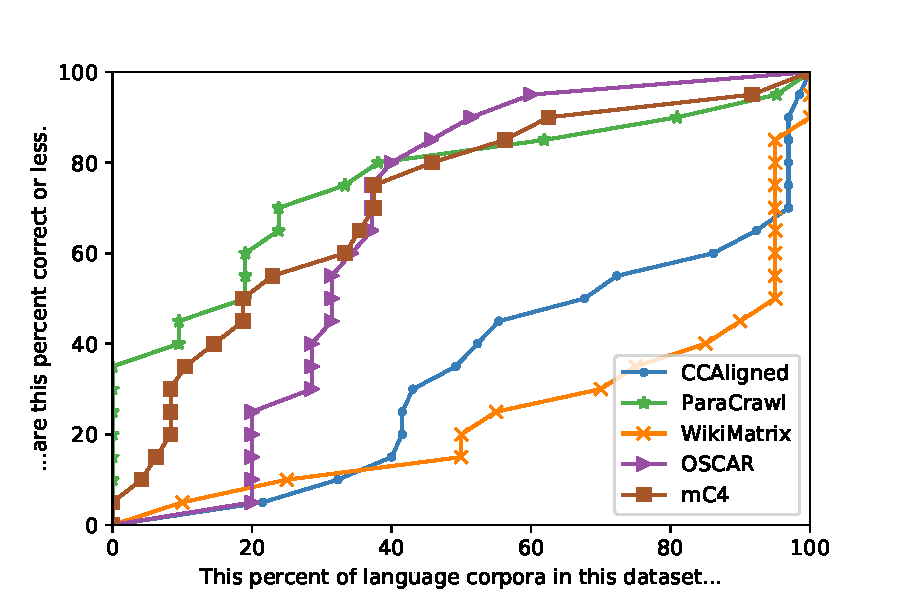
\includegraphics[width=\columnwidth]{static/media/oscar/quality/num_C_ratio.pdf}
    \caption{Fraction of languages in each dataset below a given quality threshold (percent correct).}% The larger the AUC, the better.}
    \label{fig:ratio_c}
\end{figure}

\paragraph{Why haven't these problems been reported before?}
The findings above are averaged on a per-language basis (i.e. macro-average), and therefore give low and high-resource languages equal weight. If we instead estimate the quality on a per-sentence basis, i.e. down-weight lower-resource languages in the computation of the average, the numbers paint a more optimistic picture (``micro'' block in Table~\ref{tab:results}). This is especially relevant for the monolingual datasets because they contain audits for English, which makes up for 43\% of all sentences in OSCAR 2019 and 36\% in mC4. To illustrate the effect of this imbalance: A random sample from the entire mC4 dataset with over 63\% chance will be from one of the 8 largest languages (\texttt{en}, \texttt{ru}, \texttt{es}, \texttt{de}, \texttt{fr}, \texttt{it}, \texttt{pt}, \texttt{pl}, $>$100M sentences each), %\footnote{mC4 contains 22\% \texttt{und} sentences, i.e. sentences with undefined language.} 
of which all have near perfect quality. Analogously, evaluation and tuning of web mining pipelines and resulting corpora in downstream applications focused largely on higher-resource languages (Section~\ref{sec:crawls}), so the low quality of underrepresented languages might go unnoticed if there is no dedicated evaluation, or no proficient speakers are involved in the curation~\citep{nekoto-etal-2020-participatory}.


\paragraph{How much content is nonlinguistic or in the wrong language?}
Nonlinguistic content is a more common problem than wrong-language content. Among the parallel datasets, CCAligned contains the highest percentage of nonlinguistic content, at 31.42\% on average across all rated corpora, and also the highest percent of wrong-language content, at 9.44\%. Among the monolingual datasets, mC4 contains the highest ratio both of sentences in incorrect languages (15.98\% average) and nonlinguistic content (11.40\% average), with 4 of the 48 audited languages having more than 50\% contents in other languages. The low amount of wrong language in ParaCrawl shows the benefits of selecting domains by the amount in-language text, but the dataset also covers the smallest amount of languages. The low ratio of wrong language samples in OSCAR may reflect the success of line-level LangID filtering.
These numbers provide evidence that more research in LangID could improve the overall quality, especially with respect to nonlinguistic content.

\paragraph{Which languages got confused?} The languages that were confused were frequently related higher-resource languages. However, there were also a significant number of ``out-of-model cousin" cases, where languages not supported by the LangID model ended up in a similar-seeming language. For instance in mC4, much of the Shona (\texttt{sn}, Bantu language spoken in Zimbabwe and Mozambique) corpus is actually Kinyarwanda (\texttt{rw}, Bantu language spoken in mostly in Rwanda and Uganda)---and, peculiarly, much of the Hawaiian (\texttt{haw}, Polynesian language spoken in Hawaii) is actually Twi (\texttt{tw}/\texttt{ak}, Central Tano language spoken mostly in Ghana).

\begin{figure}[th]
    \centering
    \begin{subfigure}{.5\textwidth}
        \centering
        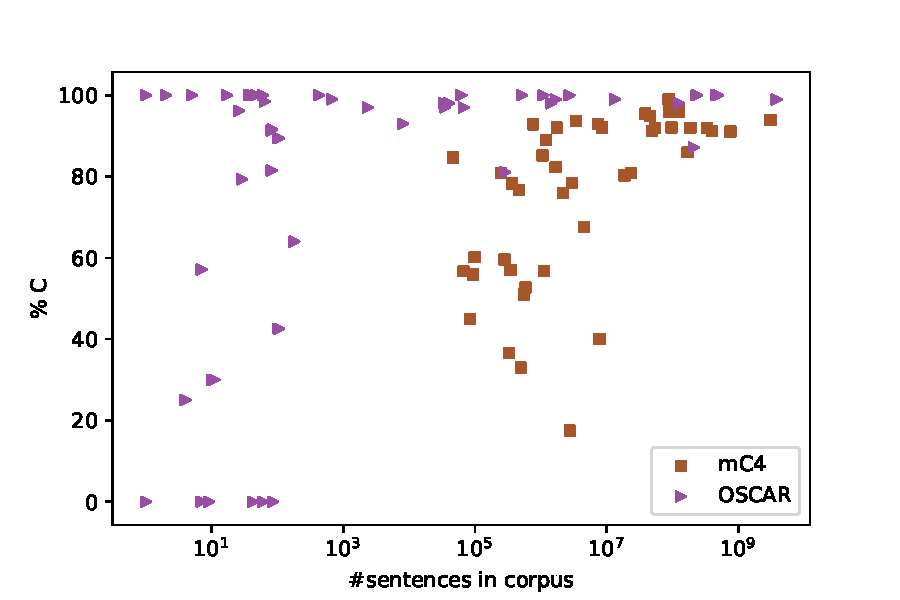
\includegraphics[width=\linewidth]{static/media/oscar/quality/C_mono.pdf}
        \caption{Monolingual corpora}
        \label{fig:C_mono}
    \end{subfigure}%
    \begin{subfigure}{.5\textwidth}
        \centering
        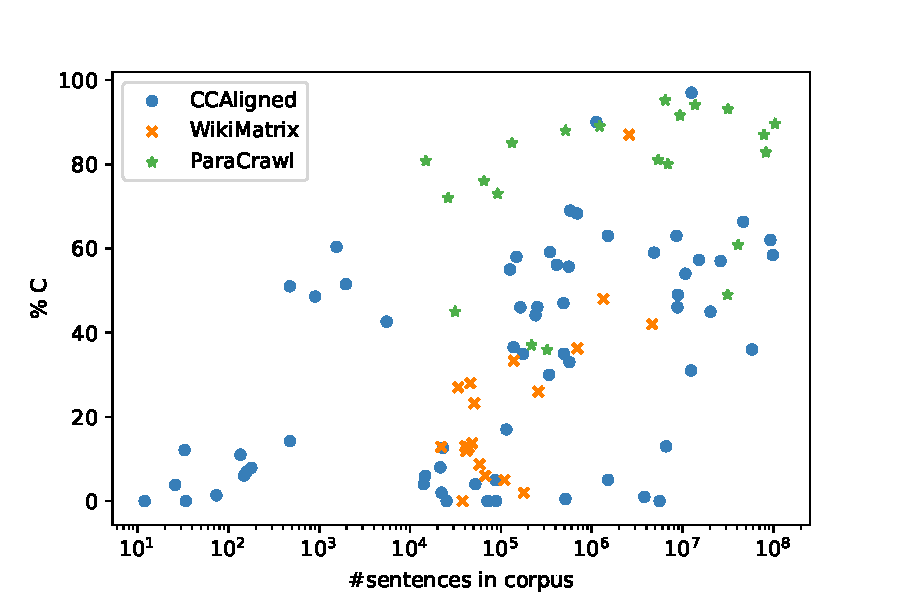
\includegraphics[width=\linewidth]{static/media/oscar/quality/C_para.pdf}
        \caption{Parallel corpora}
        \label{fig:C_para}
    \end{subfigure}
    \caption{Percentage of sentences labeled as correct vs. log N sentences for all audited languages.}
    \label{fig:C}
\end{figure}

\paragraph{Do low-resource languages have lower quality?}
Low-resource datasets tend to have lower human-judged quality.
The Spearman rank correlation between quality (\%\texttt{C}) and size is positive in all cases. The trend is strongest for mC4 ($r=0.66$), %,p=6.8e-8$), 
and gradually declines for CCAligned ($r=0.53$), %,p=0.0001$),
WikiMatrix ($r=0.49$), %,p=0.03$), 
ParaCrawl ($r=0.43$), %,p=0.02$) 
and OSCAR ($r=0.37$). %,p=0.10$).
Figure~\ref{fig:C} compares the number of sentences for each language against the proportion of correct sentences: %that we found during the audit:
%The correlation between quality (\%\texttt{C}) and size is strongest for WikiMatrix (Pearson's $r=0.66$), while mC4, CCAligned, ParaCrawl have comparatively lower correlation (0.21, 0.25, 0.29), and OSCAR the lowest with $r=0.13$.
%In general, we observe that languages with low representation tend to contain fewer correct sentences, with an exception of a dozen of languages from OSCAR.
Not all higher-resource languages ($>10^6$ sentences) have high quality, in particular for CCAligned (e.g. Javanese (\texttt{en\nobreakdash-jv\_ID}) with 5\%\texttt{C}, or Tagalog (\texttt{en\nobreakdash-tl\_XX}) with 13\%\texttt{C}). For mid-resource languages ($10^4$\nobreakdash--$10^6$ sentences) the picture is inconclusive, with some languages having high quality, and others having extremely low quality, even within the same datasets, e.g. Urdu in CCAligned \texttt{en-ur\_PK} has 100\%\texttt{C} vs. its romanized counterpart \texttt{en\nobreakdash-ur\_PK\_rom} 0.5\% \texttt{C}.
%\footnote{\texttt{\_rom} corpora have been removed in the latest CCAligned release.}
For individual error codes trends are less clear (not depicted).

\paragraph{Which languages have the lowest quality?} Across datasets we observe that the quality is particularly poor for languages that are included in romanized script (\texttt{\_rom}/\texttt{\_latn}), but are more commonly written in other scripts, e.g., Urdu (\texttt{ur}), Japanese (\texttt{ja}), Arabic (\texttt{ar}).
%\footnote{These romanized versions have been removed from CCAligned in a later release.} 
These are not transliterations of other scripts, but mostly contain non-linguistic material or wrong languages (e.g. the romanized Japanese corpus in mC4 (\texttt{ja\_latn}) contains Spanish, French, English, Portuguese, amongst others). %, Chinese (\texttt{zh}), Telugu (\texttt{te}) and Bulgarian (\texttt{bg}).  
In terms of geography, the poorest quality is found for African languages (Bambara (\texttt{bm}), Fula (\texttt{ff}), Kikongo (\texttt{kg}), Luganda (\texttt{lg}), Lingala (\texttt{ln}), Norther Sotho (\texttt{nso}), Oromo (\texttt{om}), Shona (\texttt{sn}), Somali (\texttt{so}), Tswana (\texttt{tn}), Wolof (\texttt{wo})), minority languages in Europe and the Middle East that are closely related to higher-resource languages (Azerbaijani (\texttt{az-IR}), North Frisian (\texttt{frr}), Neapolitan (\texttt{nap}), Silesian (\texttt{szl}), Zaza (\texttt{zza})), lesser spoken Chinese languages sharing a script with Mandarin (Yue (\texttt{yue}), Wu (\texttt{wuu})), four major Austronesian (Central Bikol (\texttt{bcl}), Chavacano (\texttt{cbk}), Javanese (\texttt{jv}), Sundanese (\texttt{su})), and some South-Asian languages, in particular Sinhala (\texttt{si}).
Appendix~\ref{app:stats} contains the detailed per-language statistics for all corpora.
% Omitted from above: mt

\paragraph{What is the incidence of offensive and pornographic content?}
Overall, the sampled sentences did not contain a large amount of offensive contents. However, there were notable amounts of pornographic content ($>10\%$) found in CCAligned for 11 languages. % not fully annotated: tl_XX, lt_LV ?

\begin{table}[!htbp]
    \centering
    \resizebox{\textwidth}{!}{%

        \begin{tabular}{lcccccccccccc}
            \toprule
                           & \texttt{es\_XX} & \texttt{bm\_ML} & \texttt{yo\_NG} & \texttt{tr\_TR} & \texttt{ku\_TR} & \texttt{zh\_CN} & \texttt{af\_ZA} & \texttt{jv\_ID} & \texttt{zh\_TW} & \texttt{it\_IT} & \textbf{mean} \\
            \midrule
            \textbf{Acc-6} & 0.58            & 0.73            & 0.41            & 0.45            & 0.43            & 0.55            & 0.65            & 0.55            & 0.46            & 0.55            & 0.66          \\
            \textbf{Acc-4} & 0.77            & 0.73            & 0.60            & 0.55            & 0.56            & 0.72            & 0.72            & 0.57            & 0.58            & 0.66            & 0.72          \\
            \textbf{Acc-2} & 0.91            & 0.96            & 0.72            & 0.64            & 0.71            & 0.79            & 0.77            & 0.92            & 0.81            & 0.69            & 0.79          \\
            \bottomrule
        \end{tabular}%
    }
    \caption{Rater evaluation for a subset of audits from \textbf{CCAligned} (translated from English) measured by the accuracy (Acc-$n$) of annotations by non-proficient speaker against annotations by proficient speakers.
        %$n$ indicates the granularity of the classes.  For $n=6$ all classes of the taxonomy were distinguished, for $n=4$ the \texttt{C} subclasses were combined, and for $n=2$ it is binary decision between \texttt{C} and the rest of the error classes.
    }
    \label{tab:agreement_ccaligned}
\end{table}

\begin{table}[!htbp]
    \centering\small

    \begin{tabular}{lccccccccc}
        \toprule
                       & \texttt{tyv} & \texttt{rm} & \texttt{bar} & \texttt{eml} & \texttt{zh} & \texttt{la} & \textbf{mean} \\
        \midrule
        \textbf{Acc-6} & 1.0          & 0.98        & 1.0          & 1.0          & 0.86        & 1.0         & 0.98          \\
        \textbf{Acc-4} & 1.0          & 1.0         & 1.0          & 1.0          & 0.87        & 1.0         & 0.98          \\
        \textbf{Acc-2} & 1.0          & 1.0         & 1.0          & 1.0          & 0.87        & 1.0         & 0.98          \\
        \bottomrule
    \end{tabular}%
    \caption{Rater evaluation for a subset of audits from \textbf{OSCAR 2019} measured by the accuracy (Acc-$n$) of annotations by non-proficient speaker against annotations by proficient speakers.}
    \label{tab:agreement_oscar}
\end{table}

\paragraph{Annotation quality}
For a subset of audited languages from CCAligned and OSCAR 2019 we measure the accuracy (Acc) of the labels assigned by non-proficient speakers against the labels assigned by proficient speakers for all audited sentences. This can be understood as a directed measure of annotator agreement for the special case where one rater is an expert and the other is not. Results for varying label granularity are reported in Tables~\ref{tab:agreement_ccaligned} and \ref{tab:agreement_oscar}. For $n=6$ all classes of the taxonomy were distinguished, for $n=4$ the \texttt{C} subclasses were combined, and for $n=2$ it is binary decision between \texttt{C} and the rest of the error classes. With the full 6-class taxonomy (Acc-6) we find a mean accuracy of 0.66
%($\sigma^2 =0.02$) 
for CCAligned audits, and 0.98
%($\sigma^2 =0.002$) 
for OSCAR audits. % (see appendix~\ref{app:agreement} for language-specific results).
With a binary taxonomy (Acc-2) distinguishing \texttt{C} from the rest, the accuracy further increases to 0.79
%($\sigma^2=0.01$) 
for CCAligned. This provides strong evidence that good quality annotations are not limited to those proficient in a language.

However, the significant drop of accuracy for finer-grained labels hints at that our taxonomy can be further improved, especially for parallel sentences.
The error taxonomy lacks at least one category of error, namely ``correct/in-language but unnatural".  Similarly, the definition of ``correct-short" and ``correct-boilerplate" were not understood equally by all annotators and the concept of ``correct-short" has potential issues for agglutinative languages like Turkish. Finally, it was unclear what to do with related dialects, e.g. when a sentence is ``almost correct but wrong dialect" or when it is unclear which dialect a sentence belongs to. We recommend including these categories for future audits

\subsection{Automatic Filtering}
Given the frequency of \texttt{WL} and \texttt{NL} annotations, it might be tempting to use open-source LangID models to post-filter data on a per-sentence(-pair) level, as OSCAR does. Unfortunately, this turns out to have its own issues.

\paragraph{Sentence-level n-gram LangID filtering}
We classify all sentence pairs of CCAligned with CLD3, an n-gram based LangID model. By comparing its predictions to the audit labels, we evaluate its quality on the subset of annotated samples: the classifier should detect both correct languages when the pair is annotated as \texttt{C} and \texttt{X}, and should detect incorrect languages in the pair when \texttt{WL} and \texttt{NL}. On this task, the CLD3 classifier
%\footnote{\texttt{filter=0.976 Prec, 0.962 Rec, 0.969 F1.}} 
achieves an average precision of only 40.6\%. %,
%n average accuracy of 56.4\% against our annotators across all audited sentences, 
%underlining the issues with LangID on web domain data~\citep{caswell-etal-2020-language}. %Its recall for detecting those pairs with wrong language(s) is 77.8\%, and its precision 35.9\%. 

\paragraph{Sentence-level Transformer LangID filtering}
N-gram LangID models like CLD3 have known problems. However, \citet{caswell-etal-2020-language} demonstrate that semi-supervised Transformer-based LangID models strongly out-perform them. We train a comparable Transformer-based LangID model and apply it to our annotated CCAligned data. We find that filtering noisy corpora ($<$ 50\% correct) on LangID for both source and target leads to gains in median precision, rising from 13.8\% pre-filter to 43.9\% post-filter. However, this comes at a steep cost of 77.5\% loss in recall.
The biggest winners were Lingala, whose precision climbs from 8\% to 80\%, and Oromo, which soars from 2\% to 33\% in-language. Both of these, however, come at the cost of losing 50\% of the correct in-language sentences, being reduced from ~22k sentences to 3k and 1k sentences respectively, which would likely be too small for building downstream models. The moral is that, at least at the current stage, there is no one-size-fits-all approach for sentence-level LangID filtering.


\section{Dataset Mis-labeling}
\label{sec:codes}
Standardized and unambiguous representations of language codes are important for practical data use and exchange. The standard used by most academic and industry applications is BCP-47~\citep{phillips-etal-2005-tags}, which builds off the two-letter ISO639-2 codes and three-letter ISO639\nobreakdash-3 codes, but also allows to add subtags for scripts (e.g. Hindi in Latin script: \texttt{hi-Latn}) or regional varieties (e.g. French spoken in Canada: \texttt{fr-CA}). It would enhance transparency and interoperability if adopted consistently, especially with growing language diversity in NLP.

We find a variety of errors and inconsistencies in language code usage, ranging from serious mislabelings to small transgressions against standard conventions. For this analysis, we also include the JW300~\citep{agic-vulic-2019-jw300} dataset, a multilingual dataset crawled from \url{jw.org}. %, which was otherwise not audited in this paper. 
In summary, we find 8 nonstandard codes in CCAligned, 3 in OSCAR 2019, 1 in mC4, 1 in WikiMatrix, and 70 in JW300, for 83 in total. This does not include the 59 codes affected by superset issues. %0 in ParaCrawl, 
Full details are given in Appendix~\ref{app:jw300}.

\paragraph{Inconsistent Language Codes} One common issue is simply using nonstandard or invented codes. For example, CCAligned uses only two-letter codes, so when the BCP-47 code for a language is three letters it is either shortened (e.g. \texttt{zza} $\rightarrow$ \texttt{zz}) or invented (\texttt{shn}  $\rightarrow$ \texttt{qa}). Similarly, OSCAR 2019 contains data labeled as \texttt{als} (BCP-47 for Tosk Albanian) that is actually in \texttt{gsw} (Allemannic).\footnote{This is a result of the language code used by the \href{https://en.wikipedia.org/wiki/Alemannic\_Wikipedia}{Alemannic Wikipedia} and affects any corpus or tool that uses Wikipedia data without correcting for this, like FastText.} 22 additional language codes in JW300 have similar issues, including 12 codes that start with \texttt{jw\_} but are not Javanese.

\paragraph{False Sign Languages}
12\% (48/417) of JW300
%has a much stranger problem than nonstandard codes. It has the peculiar issue that a full 12\% (48/417) of the languages it claims to cover 
carry language codes for sign languages. %While it is possible to transcribe sign languages using glosses, this is not what these corpora are. 
Instead of sign language transcripts they are texts in another high resource language, mostly English or Spanish---for example, the \texttt{en-zsl} (Zambian sign language) data is actually English-English parallel data (copies), details in Appendix~\ref{app:jw300}. This was likely caused by videos with sign language interpretation embedded on the crawled websites.\footnote{Kudos to Rebecca Knowles for this explanation.} %Details are in Appendix Table~\ref{tab:signlanguages}.


\paragraph{Mysterious supersets}
When datasets contain language codes that are supersets of other language codes, it is difficult to determine which particular language the text contains. WikiMatrix has Serbian (\texttt{sr}), Croatian (\texttt{hr}), Bosnian (\texttt{bs}), and Serbo-Croatian (\texttt{sh})---their superset.\footnote{\url{https://iso639-3.sil.org/code/hbs}}
%. And while there may be some debate whether \texttt{bs},  \texttt{hr},  \texttt{cnr},  and \texttt{sr} are different languages, \texttt{sh} (\texttt{hbs}) is by definition a superset of all of them.\footnote{https://iso639-3.sil.org/code/hbs} 
The issue of codes that are supersets of others is common enough to include a small table dedicated to it (Appendix Table~\ref{tab:supersets}).
In some cases this may not be an issue, as with Arabic, where \texttt{ar} conventionally refers to Modern Standard Arabic, even though the code technically encompasses all dialects.
%, or where \texttt{no} typically refers to Norwegian Bokm\r{a}l (\texttt{nb}), though it technically is the superset of \texttt{nb} and \texttt{nn}. 
In many cases, the nature of the data in the superset code remains a mystery.
% requiring detective work.


\paragraph{Deprecated codes} Finally, there are several deprecated codes that are used: \texttt{sh} in Wikimatrix, \texttt{iw} in mC4, \texttt{sh} and \texttt{eml} in OSCAR 2019, and \texttt{daf} in JW300.

\section{Risks of Low-Quality Data}\label{sec:risk}

\paragraph{Low quality in downstream applications}
Text corpora today are building blocks for many downstream NLP applications like question answering and text summarization---for instance, a common approach is to first train translation models on such data and then automatically translate training data for downstream models~\citep{conneau-etal-2018-xnli}. If the data used for the original systems is flawed, derived technology may fail for those languages far down the line without knowing the causes.
This risk of undesired downstream effects calls for future studies with a careful treatment of intertwined effects such as data size and domain, language-specific phenomena, evaluation data and metric biases.
%Furthermore, there are not many existing public models trained on these specific subsets of data that we can analyze. 
To give the reader a brief glimpse of the impact of data quality for the example of translation, we compare the \texttt{C}\% metric from our audit with the translation quality (sentencepiece-BLEU, spBLEU) of the multilingual translation model M2M124 for 124 languages~\citep{goyal-etal-2021-flores-101}. It was trained on WikiMatrix and CCAligned, and similar data collected with the same tools, which we expect to show similar biases. Translation quality is evaluated on the trusted, human-translated FloReS benchmark~\citep{goyal-etal-2021-flores-101}.
%For language pairs that were both covered in the WikiMatrix and the CCAligned audit, we compute an average of their \% \texttt{C} scores weighted by their size. 
For the 21 languages present in both the audit and the FloReS benchmark, we found a positive correlation (Spearman) between the data quality scores and spBLEU of $\rho=0.44$ $(p=0.041)$. This is not as large as the correlation with data size ($\rho=0.66$, $p=0.00078$), but it nonetheless helps to explain translation quality---the correlation between the product of \texttt{C}\% and data size (in other words, the expected total number of good sentences in the dataset), is the highest yet, with a value of $\rho=0.73$ $(p=0.00013)$.\footnote{For the translation from English, BLEU scores are less comparable but the trend holds nonetheless, with values of ($\rho=0.32$, $p=0.14$), ($\rho=0.74$, $p=0.000078$), and ($\rho=0.80$, $p=0.0000087$) respectively.}
% The human inspection and auditing of e.g. trained vector representations to detect possible risks and misrepresentations of a subset of languages is arguably harder than manually inspecting a few samples as we did in this work.
% As our analysis has shown, low-resource languages are disproportionately affected by such problems in automatic data curation pipelines.

\paragraph{Representation washing}
Since there are datasets which contain many low-resource languages, the community may feel a sense of progress and growing equity, despite the actual quality of the resources for these languages. %However, models often still perform poorly on NLP tasks for these languages
%Because there appear to be datasets for low-resource languages, the community may collectively feel as though progress is being made in these areas. 
Similarly, if low-quality datasets are used as benchmarks they may exaggerate model performance, making low-resource NLP appear more solved than it is---or conversely, if models perform poorly when trained with such data, it may be wrongly assumed that the task of learning models for these languages is harder than it actually is or infeasible given current resources. These effects could result in productive effort being redirected away from these tasks and languages.
%The result can be that productive effort will be directed away from these fields.

\begin{table}[t!]

    \centering\small
    \begin{tabular}{ll}
        \toprule

        \texttt{en}  & The prime minister of the \textbf{UK} is \textbf{Boris Johnson}.          \\
        \texttt{nl}  & De minister-president van \textbf{Nederland} is \textbf{Mark Rutte}.      \\
                     & \small{\texttt{en}: The prime minister of the Netherlands is Mark Rutte.} \\
        \midrule
        %\midrule
        % \texttt{en} &Sunglasses \\
        % \texttt{ig}	&ah\d{i}a Nyocha \\
        % \midrule
        \texttt{en}  & \textbf{24 March} 2018                                                    \\
        \texttt{pt}  & \textbf{14 Novembro} 2018                                                 \\
                     & \small{\texttt{en}: 14 November 2018 }                                    \\
        %\midrule
        \midrule
        % \texttt{en} &The current local time in \textbf{Sarasota} is \textbf{89} minutes ahead of apparent solar time. \\
        % \texttt{nn}	&Den lokale tiden i \textbf{Miami} er \textbf{86} minutt f\o{o}re sann soltid. \\
        \texttt{en}  & The current local time in \textbf{Sarasota} is \textbf{89} minutes.       \\
        \texttt{nn}  & Den lokale tiden i \textbf{Miami} er \textbf{86} minutt.                  \\
                     & \small{\texttt{en}: The local time in Miami is 86 minutes.}               \\
        %\midrule
        \midrule
        \texttt{en}  & In \textbf{1932} the highway was extended \textbf{north to LA}.           \\
        \texttt{bar} & \textbf{1938} is de Autobahn bei \textbf{Inglstod} fertig gstellt.        \\
                     & \small{\texttt{en}: The highway near Inglstod was completed in 1938.}     \\
        % \midrule
        % \textit{en:} He was engaged to the lawyer and actor João Lima Junior, with whom he dated from 2004 to 2006. \\
        % \textit{nds:} Ze woont in de tussentied samen met zanger en liedtiesschriever Johannes Oerding met wie ze sinds 2009 ook samen op de bühne stiet.\\
        \bottomrule
    \end{tabular}%
    \caption{Examples of ``parallel" data where the translation has a different meaning than the source, but the form looks the same. (We added translations of the non-English side.) Such data may encourage hallucinations of fake ``facts".}
    \label{tab:not_actually_parallel}
\end{table}

\paragraph{Trust in incorrect ``facts''} % and trust} %, algorithmic trust and automation bias}
We found many instances of parallel-looking sentences that are structurally and semantically similar, but not factually correct translations (Table~\ref{tab:not_actually_parallel}). They can cause models to produce plausible ``translations" that are factually wrong, but users may still trust them (\textit{algorithmic trust}) without verifying the information. %This is relevant for \textit{algorithmic trust}, when users increasingly trust the outputs of computers and ``algorithms" without verifying the information. 
Similarly, \textit{automation bias} \citep{skitka-etal-1999-does},
%from social psychology which refers to the bias of 
referring to humans favoring decisions made by automated systems over decisions made by humans, might amplify the issues of inaccurate translations caused by misalignments.
%One variant of this issue that occurs frequently in some datasets is pornographic content.
%, which in the majority of the cases we observed were parts of misaligned sentence pairs. 
%Another effect is that models trained on misaligned pornographic content may hallucinate such content, which may be disturbing to users.

\section{Future Work and Recommendations}\label{sec:recommendation}
Of the five multilingual corpora evaluated, we consistently found severe issues with quality, especially in the lower-resource languages. We rated samples of 205 languages, and found that 87 of them had under 50\% usable data, with a full 15 languages at 0\% in-language. We furthermore found consistent issues with mislabeled data and nonstandard language codes, particularly in the JW300 dataset, and identified 83 affected corpora, at least 48 of which were entirely spurious (Section~\ref{sec:codes}). While there might have been anecdotal evidence of insufficient quality for some datasets, the majority of these quality issues had not been reported, nor been investigated in depth. These issues might go unnoticed for languages that are not represented in the evaluation of the crawling methods, and cause harm in downstream applications~\citep{khayrallah-koehn-2018-impact}.

There are a variety of ways to improve both the ease and accuracy of human evaluation, as well a few classes of issues we ignored in this paper, like close dialects.
Ideally we would like to build a standard suite of automatic metrics for datasets, but more research is necessary to determine what the appropriate metrics would be. One important area missing from our analyses however is the estimated portion of a dataset which has been generated by MT~\citep{rarrick-etal-2011-mt}, LM systems, or bots/templates, as for example in the analysis of C4~\citep{dodge-etal-2021-documenting}. %A prominent example is the Lsjbot\footnote{\url{https://en.wikipedia.org/wiki/Lsjbot}} which is responsible for creating 80-90\% of content for Swedish, Cebuano and Waray Wikipedia. 
The information captured in machine-generated content might still be useful for modeling, but might falsely overrepresent typical generation patterns and introduce linguistic errors or unnatural artifacts.
% Malagasy wiktionary audit: https://meta.wikimedia.org/wiki/Requests_for_comment/Large-scale_errors_at_Malagasy_Wiktionary
%https://www.vice.com/en/article/4agamm/the-worlds-second-largest-wikipedia-is-written-almost-entirely-by-one-bot

% Finally, similar studies to this in future would do well ton work more on calibrating human raters, to ensure consistent use of error categories.

% An issue that arises with the progress in building technology for some of the languages is the retrieval of machine-generated output as in-language data. This is prominent for mid- to high-resource languages for which translation systems have reached sufficient quality for website translation, as we observed for example a significant amount of translations for Ukrainian. Non-native speakers might not have noticed them during annotations, so the problem might be even larger than we might estimate now. We leave a systematic investigation to future work. A more unexpected artifact is the retrieval of published BPE vocabularies for a range of low-resource languages, such as Sundanese.\footnote{\url{https://nlp.h-its.org/bpemb/su/su.wiki.bpe.vs100000.vocab}

We therefore strongly recommend looking at samples of any dataset before using it or releasing it to the public. As we have shown, one does not need to be proficient in a language to see when there are serious quality issues, and a quick scan of 100 sentences can be sufficient to detect major problems. Moreover, going through and annotating a small sample of data can bring actionable insights about new ways to filter or use it.

If data quality issues are found, a wide variety of techniques can be explored, like filtering on length-ratio, LangID, TF-IDF wordlists \cite{caswell-etal-2020-language} or dictionaries~\citep{kamholz-etal-2014-panlex}; to neural approaches like LM scoring \cite{axelrod-etal-2011-domain,moore-lewis-2010-intelligent,wang-etal-2018-denoising}. Unfortunately, none of these provides a quick and easy fix, especially for low-resource languages---data cleaning is no trivial task!

Noisy datasets are by no means useless, at least if they contain some desirable content. Therefore, an alternative to filtering can be documentation~\citep{bender-etal-2021-on}. This can take the form of a per-language quality score and notes about known issues,
% ({ \it``language xx has high percentage non-linguistic content'' } etc.), 
a datasheet \citep{gebru-etal-2018-datasheets} or nutrition label \citep{holland-etal-2018-the}. However, we suggest researchers not release corpora with near-zero in-language content, as this may give the mistaken impression of usable resources.

Finally, we encourage the community to continue conducting evaluations and audits of public datasets---similar to system comparison papers.

\section{Conclusions for the OSCAR Project}

While the study described in chapter \ref{chap:monolingual} showed encouraging results for the OSCAR 2019 corpus, a lot of concerns about the actual quality of the data remained unaddressed. This has addressed some of these concerns and actually showed promising results for the OSCAR corpus especially in comparison to the other four audited corpora, as OSCAR 2019 obtained the highest percentage of correct sentences as shown in table \ref{tab:results}.

However, we also acknowledge that major issues remain to be addressed as has been pointed out here and more importantly, only $0.00004\%$ of the corpus was actually audited here, meaning that potential issues with both the corpus and the pipeline might remain to be discovered. This collaboration marks thus a turning point for the OSCAR project, as it served as a platform and catalyst for both relaunching the project and start working on further versions of the corpus to the one originally published in 2019 \citep{ortiz-suarez-etal-2019-asynchronous}. The following two chapters will describe the creation of two subsequent versions of OSCAR that try to address some of the problems described here and some others that were pointed by the users of the project at both the corpus and the pipeline level.


%%% CCALIGNED %%%

\begin{table*}[hbt!]
    \centering\small
    \resizebox*{0.9\textwidth}{!}{ %\textheight}{%
        \begin{tabular}{l|rrrr|rrrr|rr}
            \toprule
            {}                      & C       & CC      & CS      & CB      & X       & WL      & NL      & porn    & \#sentences & avg target length \\
            \midrule
            \textbf{en-sz\_PL}      & 0.00\%  & 0.00\%  & 0.00\%  & 0.00\%  & 0.00\%  & 8.33\%  & 91.67\% & 0.00\%  & 12          & 71.42             \\
            \textbf{en-mt\_MT}      & 3.85\%  & 0.00\%  & 3.85\%  & 0.00\%  & 50.00\% & 26.92\% & 19.23\% & 0.00\%  & 26          & 12.58             \\
            \textbf{en-tz\_MA}      & 12.12\% & 6.06\%  & 6.06\%  & 0.00\%  & 45.45\% & 36.36\% & 6.06\%  & 0.00\%  & 33          & 57.33             \\
            \textbf{en-zz\_TR}      & 0.00\%  & 0.00\%  & 0.00\%  & 0.00\%  & 8.82\%  & 61.76\% & 29.41\% & 0.00\%  & 34          & 46.53             \\
            \textbf{en-kg\_AO}      & 1.35\%  & 0.00\%  & 1.35\%  & 0.00\%  & 14.86\% & 2.70\%  & 81.08\% & 0.00\%  & 74          & 29.20             \\
            \textbf{en-qa\_MM}      & 11.03\% & 5.88\%  & 3.68\%  & 1.47\%  & 72.06\% & 3.68\%  & 13.24\% & 0.00\%  & 136         & 55.28             \\
            \textbf{en-bm\_ML}      & 6.04\%  & 4.03\%  & 2.01\%  & 0.00\%  & 26.85\% & 6.71\%  & 60.40\% & 0.00\%  & 149         & 32.19             \\
            \textbf{en-az\_IR}      & 6.93\%  & 6.93\%  & 0.00\%  & 0.00\%  & 20.79\% & 13.86\% & 58.42\% & 0.00\%  & 158         & 115.85            \\
            \textbf{en-qd\_MM}      & 7.92\%  & 4.95\%  & 1.98\%  & 0.99\%  & 81.19\% & 3.96\%  & 6.93\%  & 0.00\%  & 179         & 60.34             \\
            en-ay\_BO               & 51.00\% & 33.00\% & 18.00\% & 0.00\%  & 29.00\% & 3.00\%  & 17.00\% & 0.00\%  & 475         & 92.19             \\
            \textbf{en-ak\_GH}      & 14.23\% & 13.60\% & 0.63\%  & 0.00\%  & 46.86\% & 19.25\% & 19.67\% & 0.00\%  & 478         & 45.85             \\
            en-st\_ZA               & 48.57\% & 42.14\% & 0.00\%  & 6.43\%  & 40.71\% & 1.43\%  & 9.29\%  & 0.00\%  & 904         & 111.83            \\
            en-ve\_ZA               & 60.40\% & 29.70\% & 21.78\% & 8.91\%  & 28.71\% & 3.96\%  & 6.93\%  & 0.00\%  & 1555        & 82.99             \\
            en-ts\_ZA               & 51.49\% & 34.65\% & 11.88\% & 4.95\%  & 40.59\% & 2.97\%  & 4.95\%  & 0.00\%  & 1967        & 73.93             \\
            en-or\_IN               & 42.61\% & 6.09\%  & 24.35\% & 12.17\% & 38.26\% & 9.57\%  & 9.57\%  & 0.00\%  & 5526        & 71.39             \\
            \textbf{en-ns\_ZA }     & 4.00\%  & 2.00\%  & 0.00\%  & 2.00\%  & 23.00\% & 15.00\% & 58.00\% & 4.00\%  & 14138       & 33.52             \\
            \textbf{en-lg\_UG}      & 6.00\%  & 0.00\%  & 6.00\%  & 0.00\%  & 68.00\% & 17.00\% & 9.00\%  & 2.00\%  & 14701       & 15.83             \\
            \textbf{en-ln\_CD}      & 8.00\%  & 4.00\%  & 3.00\%  & 1.00\%  & 14.00\% & 4.00\%  & 74.00\% & 4.00\%  & 21562       & 28.80             \\
            \textbf{en-om\_KE}      & 2.00\%  & 2.00\%  & 0.00\%  & 0.00\%  & 31.00\% & 38.00\% & 29.00\% & 24.00\% & 22206       & 23.83             \\
            \textbf{en-ss\_SZ}      & 12.65\% & 9.04\%  & 3.61\%  & 0.00\%  & 13.25\% & 24.10\% & 50.00\% & 13.86\% & 22960       & 25.30             \\
            \textbf{en-te\_IN\_rom} & 0.00\%  & 0.00\%  & 0.00\%  & 0.00\%  & 25.00\% & 8.00\%  & 67.00\% & 5.00\%  & 25272       & 24.21             \\
            \textbf{en-cb\_IQ}      & 4.00\%  & 1.00\%  & 3.00\%  & 0.00\%  & 30.00\% & 18.00\% & 48.00\% & 11.00\% & 52297       & 30.04             \\
            \textbf{en-tn\_BW}      & 0.00\%  & 0.00\%  & 0.00\%  & 0.00\%  & 6.90\%  & 8.97\%  & 63.45\% & 10.34\% & 71253       & 16.80             \\
            \textbf{en-ff\_NG}      & 0.00\%  & 0.00\%  & 0.00\%  & 0.00\%  & 0.00\%  & 8.00\%  & 92.00\% & 2.00\%  & 73022       & 33.59             \\
            \textbf{en-sn\_ZW}      & 5.00\%  & 1.00\%  & 3.00\%  & 1.00\%  & 81.00\% & 14.00\% & 0.00\%  & 0.00\%  & 86868       & 102.59            \\
            \textbf{en-wo\_SN}      & 0.00\%  & 0.00\%  & 0.00\%  & 0.00\%  & 1.71\%  & 3.31\%  & 94.98\% & 18.46\% & 88441       & 27.25             \\
            \textbf{en-br\_FR}      & 17.00\% & 3.00\%  & 1.00\%  & 13.00\% & 37.00\% & 14.00\% & 32.00\% & 1.00\%  & 115128      & 41.68             \\
            en-zu\_ZA               & 55.00\% & 39.00\% & 3.00\%  & 13.00\% & 30.00\% & 7.00\%  & 8.00\%  & 3.00\%  & 126101      & 79.32             \\
            en-ku\_TR               & 36.52\% & 12.17\% & 13.04\% & 11.30\% & 33.04\% & 28.70\% & 1.74\%  & 1.74\%  & 137874      & 90.51             \\
            en-ig\_NG               & 58.00\% & 49.00\% & 3.00\%  & 6.00\%  & 29.00\% & 12.00\% & 1.00\%  & 0.00\%  & 148146      & 83.42             \\
            en-kn\_IN               & 46.00\% & 9.00\%  & 6.00\%  & 31.00\% & 46.00\% & 2.00\%  & 5.00\%  & 4.00\%  & 163921      & 70.20             \\
            en-yo\_NG               & 34.93\% & 6.16\%  & 10.96\% & 17.81\% & 34.93\% & 12.33\% & 17.81\% & 0.00\%  & 175192      & 75.01             \\
            en-ky\_KG               & 44.12\% & 24.51\% & 17.65\% & 1.96\%  & 33.33\% & 22.55\% & 0.00\%  & 0.98\%  & 240657      & 69.56             \\
            en-tg\_TJ               & 46.08\% & 18.63\% & 24.51\% & 2.94\%  & 32.35\% & 20.59\% & 0.98\%  & 4.90\%  & 251865      & 75.31             \\
            en-ha\_NG               & 30.00\% & 25.00\% & 3.00\%  & 2.00\%  & 49.00\% & 9.00\%  & 12.00\% & 1.00\%  & 339176      & 60.78             \\
            en-am\_ET               & 59.11\% & 35.47\% & 2.46\%  & 21.18\% & 37.44\% & 2.96\%  & 0.49\%  & 0.00\%  & 346517      & 58.29             \\
            en-km\_KH               & 56.12\% & 12.24\% & 33.67\% & 10.20\% & 42.86\% & 1.02\%  & 0.00\%  & 0.00\%  & 412381      & 71.35             \\
            en-ne\_NP               & 47.00\% & 10.00\% & 13.00\% & 24.00\% & 15.00\% & 8.00\%  & 30.00\% & 14.00\% & 487155      & 79.14             \\
            en-su\_ID               & 35.00\% & 15.00\% & 15.00\% & 5.00\%  & 13.00\% & 13.00\% & 39.00\% & 0.00\%  & 494142      & 57.08             \\
            \textbf{en-ur\_PK\_rom} & 0.50\%  & 0.00\%  & 0.50\%  & 0.00\%  & 18.91\% & 27.36\% & 53.23\% & 5.47\%  & 513123      & 18.41             \\
            en-ht\_HT               & 55.67\% & 8.25\%  & 10.31\% & 37.11\% & 35.05\% & 6.19\%  & 3.09\%  & 1.03\%  & 558167      & 101.95            \\
            en-mn\_MN               & 33.00\% & 8.00\%  & 14.00\% & 11.00\% & 42.00\% & 7.00\%  & 18.00\% & 12.00\% & 566885      & 44.43             \\
            en-te\_IN               & 69.00\% & 42.00\% & 11.00\% & 16.00\% & 27.00\% & 1.00\%  & 3.00\%  & 1.00\%  & 581651      & 97.95             \\
            en-kk\_KZ               & 68.32\% & 40.59\% & 18.81\% & 8.91\%  & 18.81\% & 8.91\%  & 3.96\%  & 1.98\%  & 689651      & 72.36             \\
            en-be\_BY               & 90.00\% & 57.00\% & 13.00\% & 20.00\% & 10.00\% & 0.00\%  & 0.00\%  & 2.00\%  & 1125772     & 118.45            \\
            en-af\_ZA               & 63.00\% & 40.00\% & 23.00\% & 0.00\%  & 31.00\% & 2.00\%  & 4.00\%  & 12.00\% & 1504061     & 105.45            \\
            \textbf{en-jv\_ID}      & 5.05\%  & 1.01\%  & 1.01\%  & 3.03\%  & 25.25\% & 10.10\% & 59.60\% & 8.08\%  & 1513974     & 18.34             \\

            \textbf{en-hi\_IN\_rom} & 1.00\%  & 0.00\%  & 0.00\%  & 1.00\%  & 39.00\% & 21.00\% & 39.00\% & 8.00\%  & 3789571     & 18.13             \\
            en-lv\_LV               & 59.00\% & 37.00\% & 9.00\%  & 13.00\% & 31.00\% & 7.00\%  & 3.00\%  & 14.00\% & 4850957     & 83.67             \\
            \textbf{en-ar\_AR\_rom} & 0.00\%  & 0.00\%  & 0.00\%  & 0.00\%  & 0.00\%  & 4.00\%  & 96.00\% & 4.00\%  & 5584724     & 16.69             \\
            \textbf{en-tl\_XX}      & 13.00\% & 6.00\%  & 3.00\%  & 4.00\%  & 24.00\% & 26.00\% & 37.00\% & 5.00\%  & 6593250     & 37.03             \\
            en-uk\_UA               & 63.00\% & 42.00\% & 8.00\%  & 13.00\% & 35.00\% & 1.00\%  & 1.00\%  & 5.00\%  & 8547348     & 67.88             \\
            en-zh\_TW               & 46.00\% & 11.00\% & 31.00\% & 4.00\%  & 47.00\% & 6.00\%  & 1.00\%  & 1.00\%  & 8778971     & 24.89             \\
            en-el\_GR               & 49.00\% & 15.00\% & 5.00\%  & 29.00\% & 38.00\% & 3.00\%  & 10.00\% & 8.00\%  & 8878492     & 54.90             \\
            en-nl\_NL               & 46.00\% & 27.00\% & 19.00\% & 0.00\%  & 49.00\% & 2.00\%  & 3.00\%  & 0.00\%  & 36324231    & 85.95             \\
            en-da\_DK               & 54.00\% & 31.00\% & 18.00\% & 5.00\%  & 29.00\% & 5.00\%  & 12.00\% & 7.00\%  & 10738582    & 73.99             \\
            en-vi\_VN               & 31.00\% & 18.00\% & 0.00\%  & 13.00\% & 54.00\% & 1.00\%  & 14.00\% & 6.00\%  & 12394379    & 74.19             \\
            en-sv\_SE               & 97.00\% & 91.00\% & 3.00\%  & 3.00\%  & 0.00\%  & 3.00\%  & 0.00\%  & 0.00\%  & 12544075    & 103.91            \\
            en-zh\_CN               & 57.29\% & 22.92\% & 12.50\% & 21.88\% & 31.25\% & 1.04\%  & 10.42\% & 1.04\%  & 15181410    & 33.55             \\
            en-tr\_TR               & 45.00\% & 14.50\% & 14.00\% & 16.50\% & 44.50\% & 5.00\%  & 5.50\%  & 4.00\%  & 20282339    & 83.80             \\
            en-ja\_XX               & 57.00\% & 35.00\% & 21.00\% & 1.00\%  & 34.00\% & 6.00\%  & 0.00\%  & 0.00\%  & 26201214    & 34.44             \\
            en-pt\_XX               & 66.34\% & 36.63\% & 10.89\% & 18.81\% & 20.79\% & 3.96\%  & 8.91\%  & 0.00\%  & 46525410    & 87.20             \\
            en-it\_IT               & 36.00\% & 14.00\% & 18.00\% & 4.00\%  & 60.00\% & 1.00\%  & 3.00\%  & 0.00\%  & 58022366    & 97.44             \\
            en-de\_DE               & 62.00\% & 29.00\% & 14.00\% & 19.00\% & 28.00\% & 2.00\%  & 8.00\%  & 2.00\%  & 92597196    & 78.08             \\
            en-es\_XX               & 58.42\% & 16.83\% & 25.74\% & 15.84\% & 22.77\% & 2.97\%  & 15.84\% & 4.95\%  & 98351611    & 72.18             \\
            %\midrule
            %\textit{mean} & 27.01\% & 29.35\% & 8.62\% & 28.97\% & 14.48\% & 6.49\% & 5.89\% &     0.00\% & 5.26\% & \\
            %nl  36324231 after id_ID \\
            \bottomrule
        \end{tabular}%
    }
    \caption{Audit results for a sample of 100 sentences from \textbf{CCAligned} for each language pair, compared to the number of sentences available in the dataset. If fewer than 100 sentences were available, all sentences were audited. Language codes are as originally published.  The length is measured in number of characters and averaged across the audited portion of each corpus. Languages with less than 20\% correct sentences are boldfaced.}

    \label{tab:ccaligned-full}
\end{table*}

% template frame:
%\begin{table*}
%\centering
%\resizebox*{0.8\textwidth}{\textheight}{%
% [INSERT TABLE]
%}
%\caption{Audit results for a sample of 100 sentences from CCAligned for each language.}
%\end{table*}

\clearpage

%%% WIKIMATRIX %%%
\begin{table*}[hbt!]
    \centering
    \resizebox{0.9\textwidth}{!}{%
        \begin{tabular}{l|rrrr|rrrr|rr}
            \toprule
            {}               & C       & CC      & CS     & CB      & X       & WL      & NL     & porn   & \# sentences & avg target length \\
            \midrule
            \textbf{en-ug}   & 12.87\% & 8.91\%  & 1.98\% & 1.98\%  & 72.28\% & 9.90\%  & 1.98\% & 0.00\% & 22012        & 95.55             \\
            en-mwl           & 27.00\% & 26.00\% & 0.00\% & 1.00\%  & 73.00\% & 0.00\%  & 0.00\% & 0.00\% & 33899        & 135.26            \\
            \textbf{en-tg}   & 0.00\%  & 0.00\%  & 0.00\% & 0.00\%  & 95.10\% & 3.92\%  & 0.98\% & 0.00\% & 37975        & 88.87             \\
            \textbf{en-ne}   & 13.00\% & 7.00\%  & 6.00\% & 0.00\%  & 60.00\% & 23.00\% & 4.00\% & 0.00\% & 40549        & 69.26             \\
            \textbf{en-ka}   & 11.88\% & 2.97\%  & 2.97\% & 5.94\%  & 73.27\% & 10.89\% & 2.97\% & 0.00\% & 41638        & 144.74            \\
            \textbf{en-lmo } & 12.75\% & 11.76\% & 0.00\% & 0.98\%  & 81.37\% & 4.90\%  & 0.98\% & 0.00\% & 43790        & 89.38             \\
            en-io            & 28.00\% & 27.00\% & 0.00\% & 1.00\%  & 69.00\% & 2.00\%  & 1.00\% & 0.00\% & 45999        & 83.26             \\
            \textbf{en-jv}   & 13.73\% & 9.80\%  & 0.00\% & 3.92\%  & 70.59\% & 12.75\% & 2.94\% & 0.00\% & 48301        & 91.87             \\
            en-wuu           & 23.23\% & 14.14\% & 7.07\% & 2.02\%  & 65.66\% & 7.07\%  & 4.04\% & 0.00\% & 51024        & 34.77             \\
            \textbf{br-en}   & 8.70\%  & 7.61\%  & 1.09\% & 0.00\%  & 82.61\% & 4.35\%  & 0.00\% & 0.00\% & 58400        & 90.68             \\
            \textbf{bar-en}  & 6.00\%  & 6.00\%  & 0.00\% & 0.00\%  & 75.00\% & 16.00\% & 3.00\% & 0.00\% & 67394        & 103.51            \\
            \textbf{en-kk}   & 5.00\%  & 2.00\%  & 2.00\% & 1.00\%  & 81.00\% & 14.00\% & 0.00\% & 0.00\% & 109074       & 56.03             \\
            en-sw            & 33.33\% & 27.27\% & 4.04\% & 2.02\%  & 64.65\% & 2.02\%  & 0.00\% & 0.00\% & 138590       & 111.61            \\
            \textbf{en-nds}  & 1.96\%  & 1.96\%  & 0.00\% & 0.00\%  & 95.10\% & 1.96\%  & 0.98\% & 0.00\% & 178533       & 91.95             \\
            be-en            & 26.00\% & 24.00\% & 2.00\% & 0.00\%  & 73.00\% & 1.00\%  & 0.00\% & 0.00\% & 257946       & 121.22            \\
            en-hi            & 36.27\% & 32.35\% & 0.98\% & 2.94\%  & 59.80\% & 0.98\%  & 2.94\% & 0.00\% & 696125       & 96.77             \\
            en-ko            & 48.04\% & 33.33\% & 2.94\% & 11.76\% & 48.04\% & 2.94\%  & 0.98\% & 0.00\% & 1345630      & 55.18             \\
            en-uk            & 87.00\% & 84.00\% & 2.00\% & 1.00\%  & 10.00\% & 1.00\%  & 2.00\% & 0.00\% & 2576425      & 104.39            \\
            en-it            & 42.00\% & 42.00\% & 0.00\% & 0.00\%  & 58.00\% & 0.00\%  & 0.00\% & 0.00\% & 4626048      & 140.27            \\
            en-simple        & 37.62\% & 24.75\% & 0.00\% & 12.87\% & 56.44\% & 2.97\%  & 2.97\% & 0.00\% & N/A          & 77.53             \\
            \bottomrule
        \end{tabular}%
    }
    \caption{Audit results for a sample of 100 sentences from \textbf{WikiMatrix} for each language pair, compared to the number of sentences available in the dataset. Language codes are as originally published. The length is measured in number of characters and averaged across the audited portion of each corpus. Languages with less than 20\% correct sentences are boldfaced.}

    \label{tab:wikimatrix-full}
\end{table*}


%%% PARACRAWL %%%
\begin{table*}[hbt!]
    \centering
    \resizebox{0.9\textwidth}{!}{%
        \begin{tabular}{l|rrrr|rrrr|rr}
            \toprule
            {}    & C       & CC      & CS      & CB      & X       & WL      & NL      & porn   & \# sentences & avg target length \\
            \midrule
            en-so & 80.81\% & 61.62\% & 1.01\%  & 18.18\% & 14.14\% & 5.05\%  & 0.00\%  & 0.00\% & 14879        & 189.83            \\
            en-ps & 72.00\% & 53.00\% & 9.00\%  & 10.00\% & 17.00\% & 10.00\% & 0.00\%  & 0.00\% & 26321        & 141.01            \\
            en-my & 45.00\% & 9.00\%  & 16.00\% & 20.00\% & 32.00\% & 9.00\%  & 14.00\% & 0.00\% & 31374        & 147.07            \\
            en-km & 76.00\% & 51.00\% & 13.00\% & 12.00\% & 18.00\% & 6.00\%  & 0.00\%  & 0.00\% & 65113        & 121.20            \\
            en-ne & 73.00\% & 48.00\% & 1.00\%  & 24.00\% & 23.00\% & 2.00\%  & 0.00\%  & 0.00\% & 92084        & 153.42            \\
            en-sw & 85.00\% & 60.00\% & 15.00\% & 10.00\% & 11.00\% & 2.00\%  & 2.00\%  & 0.00\% & 132517       & 167.34            \\
            en-si & 37.00\% & 31.00\% & 6.00\%  & 0.00\%  & 62.00\% & 0.00\%  & 1.00\%  & 0.00\% & 217407       & 123.06            \\
            en-nn & 35.92\% & 24.27\% & 8.74\%  & 2.91\%  & 49.51\% & 13.59\% & 0.97\%  & 0.00\% & 323519       & 56.24             \\
            es-eu & 88.00\% & 66.00\% & 15.00\% & 7.00\%  & 10.00\% & 1.00\%  & 1.00\%  & 0.00\% & 514610       & 121.31            \\
            es-gl & 89.00\% & 46.00\% & 6.00\%  & 37.00\% & 4.00\%  & 7.00\%  & 0.00\%  & 0.00\% & 1222837      & 107.88            \\
            en-ru & 81.00\% & 73.00\% & 6.00\%  & 2.00\%  & 19.00\% & 0.00\%  & 0.00\%  & 6.00\% & 5377911      & 101.28            \\
            en-bg & 95.15\% & 85.44\% & 0.97\%  & 8.74\%  & 4.85\%  & 0.00\%  & 0.00\%  & 0.97\% & 6470710      & 112.29            \\
            es-ca & 80.00\% & 54.00\% & 19.00\% & 7.00\%  & 11.00\% & 9.00\%  & 0.00\%  & 5.00\% & 6870183      & 107.21            \\
            en-el & 91.59\% & 68.22\% & 0.93\%  & 22.43\% & 7.48\%  & 0.93\%  & 0.00\%  & 0.00\% & 9402646      & 135.66            \\
            en-pl & 94.12\% & 76.47\% & 0.98\%  & 16.67\% & 3.92\%  & 1.96\%  & 0.00\%  & 0.98\% & 13744860     & 95.95             \\
            en-nl & 49.00\% & 32.00\% & 17.00\% & 0.00\%  & 46.00\% & 3.00\%  & 2.00\%  & 0.00\% & 31295016     & 95.05             \\
            en-pt & 93.07\% & 92.08\% & 0.00\%  & 0.99\%  & 4.95\%  & 1.98\%  & 0.00\%  & 0.00\% & 31486963     & 108.68            \\
            en-it & 60.82\% & 36.08\% & 16.49\% & 8.25\%  & 38.14\% & 0.00\%  & 1.03\%  & 0.00\% & 40798278     & 127.55            \\
            en-es & 87.00\% & 54.00\% & 20.00\% & 13.00\% & 12.00\% & 0.00\%  & 1.00\%  & 0.50\% & 78662122     & 119.72            \\
            en-de & 82.83\% & 64.65\% & 13.13\% & 5.05\%  & 13.13\% & 3.03\%  & 1.01\%  & 0.00\% & 82638202     & 111.43            \\
            en-fr & 89.62\% & 82.08\% & 4.72\%  & 2.83\%  & 10.38\% & 0.00\%  & 0.00\%  & 0.00\% & 104351522    & 144.20            \\
            \bottomrule
        \end{tabular} %
    }
    \caption{Audit results for a sample of 100 sentences from \textbf{ParaCrawl} for each language pair, compared to the number of sentences available in the dataset. Language codes are as originally published.  The length is measured in number of characters and averaged across the audited portion of each corpus.}
    \label{tab:paracrawl-full}
\end{table*}

\clearpage


%%% mC4 %%%

\begin{table*}[hbt!]
    \centering
    \resizebox*{0.9\textwidth}{!}{%
        \begin{tabular}{l|rrrr|rrr|rr}
            \toprule
            {}                & C       & CC      & CS      & CB      & WL      & NL      & porn   & \# sentences & avg length \\
            \midrule
            yo                & 84.69\% & 71.43\% & 2.04\%  & 11.22\% & 14.29\% & 1.02\%  & 0.00\% & 46214        & 117.71     \\
            st                & 56.70\% & 42.27\% & 14.43\% & 0.00\%  & 35.05\% & 8.25\%  & 0.00\% & 66837        & 132.13     \\
            haw               & 44.90\% & 34.69\% & 1.02\%  & 9.18\%  & 33.67\% & 21.43\% & 1.02\% & 84312        & 129.99     \\
            ig                & 55.91\% & 41.73\% & 10.24\% & 3.94\%  & 0.00\%  & 44.09\% & 0.79\% & 92909        & 98.03      \\
            sm                & 60.20\% & 58.16\% & 2.04\%  & 0.00\%  & 27.55\% & 12.24\% & 0.00\% & 98467        & 126.42     \\
            ha                & 80.81\% & 79.80\% & 1.01\%  & 0.00\%  & 14.14\% & 5.05\%  & 2.02\% & 247479       & 155.76     \\
            su                & 59.60\% & 58.59\% & 1.01\%  & 0.00\%  & 25.25\% & 15.15\% & 2.02\% & 280719       & 107.10     \\
            sn                & 36.63\% & 32.67\% & 2.97\%  & 0.99\%  & 58.42\% & 4.95\%  & 0.00\% & 326392       & 145.59     \\
            mg                & 57.00\% & 57.00\% & 0.00\%  & 0.00\%  & 18.00\% & 25.00\% & 0.00\% & 345040       & 116.23     \\
            pa                & 78.30\% & 68.87\% & 3.77\%  & 5.66\%  & 4.72\%  & 10.38\% & 0.00\% & 363399       & 134.43     \\
            ga                & 76.77\% & 58.59\% & 6.06\%  & 12.12\% & 10.10\% & 13.13\% & 0.00\% & 465670       & 147.35     \\
            co                & 33.00\% & 29.00\% & 2.00\%  & 2.00\%  & 48.00\% & 19.00\% & 0.00\% & 494913       & 195.30     \\
            zu                & 51.00\% & 48.00\% & 2.00\%  & 1.00\%  & 30.00\% & 19.00\% & 0.00\% & 555458       & 137.81     \\
            jv                & 52.73\% & 19.09\% & 19.09\% & 14.55\% & 40.00\% & 7.27\%  & 1.82\% & 581528       & 97.96      \\
            km                & 92.86\% & 92.86\% & 0.00\%  & 0.00\%  & 7.14\%  & 0.00\%  & 0.00\% & 756612       & 162.57     \\
            kn                & 85.15\% & 73.27\% & 3.96\%  & 7.92\%  & 2.97\%  & 9.90\%  & 0.00\% & 1056849      & 105.39     \\
            fy                & 56.73\% & 50.00\% & 3.85\%  & 2.88\%  & 39.42\% & 3.85\%  & 0.00\% & 1104359      & 234.25     \\
            te                & 89.00\% & 76.00\% & 9.00\%  & 4.00\%  & 3.00\%  & 8.00\%  & 0.00\% & 1188243      & 108.49     \\
            la                & 82.31\% & 65.38\% & 6.15\%  & 10.77\% & 10.00\% & 7.69\%  & 0.00\% & 1674463      & 67.25      \\
            be                & 92.04\% & 86.73\% & 2.65\%  & 2.65\%  & 4.42\%  & 3.54\%  & 0.00\% & 1742030      & 110.86     \\
            af                & 76.00\% & 76.00\% & 0.00\%  & 0.00\%  & 15.00\% & 9.00\%  & 0.00\% & 2152243      & 99.52      \\
            \textbf{lb}       & 17.48\% & 17.48\% & 0.00\%  & 0.00\%  & 7.77\%  & 74.76\% & 0.00\% & 2740336      & 481.68     \\
            ne                & 78.35\% & 77.32\% & 1.03\%  & 0.00\%  & 21.65\% & 0.00\%  & 0.00\% & 2942785      & 102.88     \\
            sr                & 93.69\% & 85.59\% & 7.21\%  & 0.90\%  & 5.41\%  & 0.00\%  & 0.00\% & 3398483      & 131.72     \\
            gl                & 67.62\% & 57.14\% & 10.48\% & 0.00\%  & 13.33\% & 17.14\% & 0.00\% & 4549465      & 151.45     \\
            bn                & 93.00\% & 86.00\% & 1.00\%  & 6.00\%  & 3.00\%  & 4.00\%  & 0.00\% & 7444098      & 92.60      \\
            mr                & 40.00\% & 35.24\% & 2.86\%  & 1.90\%  & 49.52\% & 10.48\% & 0.00\% & 7774331      & 281.94     \\
            sl                & 92.08\% & 82.18\% & 4.95\%  & 4.95\%  & 2.97\%  & 4.95\%  & 0.00\% & 8499456      & 149.45     \\
            hi                & 80.30\% & 76.77\% & 1.01\%  & 2.53\%  & 19.70\% & 0.00\%  & 2.53\% & 18507273     & 105.54     \\
            bg                & 80.90\% & 75.88\% & 2.51\%  & 2.51\%  & 2.01\%  & 17.09\% & 0.00\% & 23409799     & 93.86      \\
            uk                & 95.48\% & 81.41\% & 7.54\%  & 6.53\%  & 2.01\%  & 2.51\%  & 0.00\% & 38556465     & 116.79     \\
            ro                & 94.95\% & 78.79\% & 12.12\% & 4.04\%  & 3.03\%  & 2.02\%  & 0.00\% & 45738857     & 130.08     \\
            sv                & 91.18\% & 84.31\% & 2.94\%  & 3.92\%  & 4.90\%  & 3.92\%  & 1.96\% & 48570979     & 114.45     \\
            zh                & 92.00\% & 87.00\% & 1.00\%  & 4.00\%  & 1.00\%  & 7.00\%  & 0.00\% & 54542308     & 94.77      \\
            ja                & 99.00\% & 89.00\% & 6.00\%  & 4.00\%  & 0.00\%  & 1.00\%  & 1.00\% & 87337884     & 59.94      \\
            tr                & 95.96\% & 88.89\% & 0.00\%  & 7.07\%  & 3.54\%  & 0.51\%  & 0.00\% & 87595290     & 152.75     \\
            nl                & 92.08\% & 85.15\% & 6.93\%  & 0.00\%  & 1.98\%  & 5.94\%  & 0.00\% & 96210458     & 103.67     \\
            pl                & 96.00\% & 82.00\% & 7.00\%  & 7.00\%  & 2.00\%  & 2.00\%  & 0.00\% & 126164277    & 170.70     \\
            pt                & 86.00\% & 79.00\% & 4.00\%  & 3.00\%  & 2.00\%  & 12.00\% & 1.00\% & 169239084    & 133.51     \\
            it                & 92.00\% & 79.00\% & 9.00\%  & 4.00\%  & 1.00\%  & 7.00\%  & 0.00\% & 186404508    & 180.26     \\
            fr                & 92.00\% & 82.00\% & 7.00\%  & 3.00\%  & 1.00\%  & 7.00\%  & 0.00\% & 332674575    & 143.69     \\
            de                & 91.18\% & 77.45\% & 7.84\%  & 5.88\%  & 6.86\%  & 1.96\%  & 0.00\% & 397006993    & 107.71     \\
            ru                & 91.06\% & 69.11\% & 11.38\% & 10.57\% & 4.07\%  & 4.88\%  & 0.00\% & 755585265    & 109.28     \\
            en                & 93.94\% & 83.84\% & 8.08\%  & 2.02\%  & 1.01\%  & 5.05\%  & 0.00\% & 3079081989   & 130.97     \\
            \textbf{bg\_latn} & 9.09\%  & 9.09\%  & 0.00\%  & 0.00\%  & 51.52\% & 39.39\% & 1.01\% & N/A          & 139.92     \\
            \textbf{ja\_latn} & 13.00\% & 7.00\%  & 4.00\%  & 2.00\%  & 60.00\% & 27.00\% & 0.00\% & N/A          & 218.92     \\
            ru\_latn          & 36.45\% & 25.23\% & 10.28\% & 0.93\%  & 34.58\% & 28.97\% & 0.93\% & N/A          & 123.14     \\
            \textbf{zh\_latn} & 5.00\%  & 4.00\%  & 1.00\%  & 0.00\%  & 64.00\% & 31.00\% & 0.00\% & N/A          & 186.84     \\
            \bottomrule
        \end{tabular}%
    }
    \caption{Audit results for a sample of 100 sentences from \textbf{mC4} for each language, compared to the number of sentences available in the dataset. Language codes are as originally published. The length is measured in number of characters and averaged across the audited portion of each corpus. Languages with less than 20\% correct sentences are boldfaced.}
    \label{tab:mc4-full}
\end{table*}
\clearpage


%%% OSCAR %%%
\begin{table*}[hbt!]
    \centering
    \resizebox*{0.9\textwidth}{!}{%
        \begin{tabular}{l|rrrr|rrr|rr}
            \toprule
            {}           & C        & CC       & CS     & CB      & WL       & NL       & porn   & \# sentences & avg length \\
            \midrule
            diq          & 100.00\% & 100.00\% & 0.00\% & 0.00\%  & 0.00\%   & 0.00\%   & 0.00\% & 1            & 131.00     \\
            \textbf{bcl} & 0.00\%   & 0.00\%   & 0.00\% & 0.00\%  & 0.00\%   & 100.00\% & 0.00\% & 1            & 623.00     \\
            \textbf{cbk} & 0.00\%   & 0.00\%   & 0.00\% & 0.00\%  & 100.00\% & 0.00\%   & 0.00\% & 1            & 519.00     \\
            pam          & 100.00\% & 100.00\% & 0.00\% & 0.00\%  & 0.00\%   & 0.00\%   & 0.00\% & 2            & 139.00     \\
            bar          & 25.00\%  & 25.00\%  & 0.00\% & 0.00\%  & 0.00\%   & 75.00\%  & 0.00\% & 4            & 53.50      \\
            myv          & 100.00\% & 100.00\% & 0.00\% & 0.00\%  & 0.00\%   & 0.00\%   & 0.00\% & 5            & 127.00     \\
            \textbf{yue} & 0.00\%   & 0.00\%   & 0.00\% & 0.00\%  & 57.14\%  & 42.86\%  & 0.00\% & 7            & 177.00     \\
            mwl          & 57.14\%  & 57.14\%  & 0.00\% & 0.00\%  & 42.86\%  & 0.00\%   & 0.00\% & 7            & 141.00     \\
            \textbf{frr} & 0.00\%   & 0.00\%   & 0.00\% & 0.00\%  & 0.00\%   & 100.00\% & 0.00\% & 9            & 231.56     \\
            ht           & 30.00\%  & 30.00\%  & 0.00\% & 0.00\%  & 0.00\%   & 70.00\%  & 0.00\% & 10           & 329.10     \\
            ie           & 30.00\%  & 30.00\%  & 0.00\% & 0.00\%  & 30.00\%  & 40.00\%  & 0.00\% & 11           & 121.70     \\
            scn          & 100.00\% & 100.00\% & 0.00\% & 0.00\%  & 0.00\%   & 0.00\%   & 0.00\% & 17           & 155.59     \\
            tyv          & 96.15\%  & 96.15\%  & 0.00\% & 0.00\%  & 0.00\%   & 3.85\%   & 0.00\% & 26           & 167.96     \\
            mai          & 79.31\%  & 75.86\%  & 0.00\% & 3.45\%  & 20.69\%  & 0.00\%   & 0.00\% & 29           & 141.17     \\
            bxr          & 100.00\% & 100.00\% & 0.00\% & 0.00\%  & 0.00\%   & 0.00\%   & 0.00\% & 37           & 160.76     \\
            dsb          & 100.00\% & 97.56\%  & 0.00\% & 2.44\%  & 0.00\%   & 0.00\%   & 0.00\% & 41           & 155.15     \\
            \textbf{so}  & 0.00\%   & 0.00\%   & 0.00\% & 0.00\%  & 28.57\%  & 71.43\%  & 0.00\% & 42           & 208.24     \\
            rm           & 100.00\% & 100.00\% & 0.00\% & 0.00\%  & 0.00\%   & 0.00\%   & 0.00\% & 47           & 137.66     \\
            nah          & 100.00\% & 96.67\%  & 0.00\% & 3.33\%  & 0.00\%   & 0.00\%   & 0.00\% & 60           & 164.53     \\
            \textbf{nap} & 0.00\%   & 0.00\%   & 0.00\% & 0.00\%  & 0.00\%   & 100.00\% & 0.00\% & 61           & 152.11     \\
            yo           & 98.46\%  & 96.92\%  & 0.00\% & 1.54\%  & 1.54\%   & 0.00\%   & 0.00\% & 64           & 281.57     \\
            gn           & 81.48\%  & 81.48\%  & 0.00\% & 0.00\%  & 2.47\%   & 16.05\%  & 0.00\% & 81           & 234.95     \\
            vec          & 91.36\%  & 91.36\%  & 0.00\% & 0.00\%  & 0.00\%   & 8.64\%   & 0.00\% & 81           & 184.90     \\
            kw           & 91.57\%  & 90.36\%  & 0.00\% & 1.20\%  & 3.61\%   & 4.82\%   & 0.00\% & 83           & 162.75     \\
            \textbf{wuu} & 0.00\%   & 0.00\%   & 0.00\% & 0.00\%  & 98.84\%  & 1.16\%   & 0.00\% & 86           & 157.15     \\
            eml          & 42.57\%  & 42.57\%  & 0.00\% & 0.00\%  & 0.00\%   & 57.43\%  & 0.00\% & 104          & 177.88     \\
            bh           & 89.42\%  & 21.15\%  & 0.00\% & 68.27\% & 1.92\%   & 8.65\%   & 0.00\% & 104          & 137.17     \\
            min          & 64.00\%  & 6.00\%   & 0.00\% & 58.00\% & 27.00\%  & 9.00\%   & 0.00\% & 180          & 649.85     \\
            qu           & 100.00\% & 98.97\%  & 0.00\% & 1.03\%  & 0.00\%   & 0.00\%   & 0.00\% & 425          & 167.27     \\
            su           & 99.00\%  & 99.00\%  & 0.00\% & 0.00\%  & 0.00\%   & 1.00\%   & 0.00\% & 676          & 221.00     \\
            jv           & 97.00\%  & 86.00\%  & 0.00\% & 11.00\% & 1.00\%   & 2.00\%   & 0.00\% & 2350         & 203.08     \\
            als          & 93.00\%  & 93.00\%  & 0.00\% & 0.00\%  & 6.00\%   & 1.00\%   & 0.00\% & 7997         & 375.44     \\
            la           & 98.00\%  & 98.00\%  & 0.00\% & 0.00\%  & 2.00\%   & 0.00\%   & 0.00\% & 33838        & 224.11     \\
            uz           & 98.00\%  & 98.00\%  & 0.00\% & 0.00\%  & 2.00\%   & 0.00\%   & 0.00\% & 34244        & 369.99     \\
            nds          & 97.03\%  & 95.05\%  & 0.00\% & 1.98\%  & 2.97\%   & 0.00\%   & 0.00\% & 35032        & 344.74     \\
            sw           & 98.00\%  & 98.00\%  & 0.00\% & 0.00\%  & 0.00\%   & 2.00\%   & 0.00\% & 40066        & 196.70     \\
            br           & 100.00\% & 96.00\%  & 0.00\% & 4.00\%  & 0.00\%   & 0.00\%   & 0.00\% & 61941        & 239.56     \\
            fy           & 97.00\%  & 97.00\%  & 0.00\% & 0.00\%  & 2.00\%   & 1.00\%   & 0.00\% & 67762        & 340.23     \\
            am           & 81.09\%  & 79.10\%  & 0.00\% & 1.99\%  & 18.91\%  & 0.00\%   & 0.00\% & 287142       & 267.43     \\
            af           & 100.00\% & 100.00\% & 0.00\% & 0.00\%  & 0.00\%   & 0.00\%   & 0.00\% & 517353       & 339.18     \\
            eu           & 100.00\% & 98.00\%  & 0.00\% & 2.00\%  & 0.00\%   & 0.00\%   & 0.00\% & 1099498      & 330.93     \\
            mn           & 98.00\%  & 94.00\%  & 0.00\% & 4.00\%  & 2.00\%   & 0.00\%   & 0.00\% & 1430527      & 309.94     \\
            te           & 98.99\%  & 93.94\%  & 1.01\% & 4.04\%  & 0.00\%   & 1.01\%   & 1.01\% & 1685185      & 412.31     \\
            kk           & 100.00\% & 100.00\% & 0.00\% & 0.00\%  & 0.00\%   & 0.00\%   & 0.00\% & 2719851      & 318.93     \\
            ca           & 99.00\%  & 91.00\%  & 0.00\% & 8.00\%  & 1.00\%   & 0.00\%   & 0.00\% & 13292843     & 333.38     \\
            nl           & 98.00\%  & 94.00\%  & 2.00\% & 2.00\%  & 2.00\%   & 0.00\%   & 4.00\% & 126067610    & 305.01     \\
            it           & 87.13\%  & 71.29\%  & 1.98\% & 13.86\% & 11.88\%  & 0.99\%   & 1.98\% & 210348435    & 393.66     \\
            zh           & 100.00\% & 97.00\%  & 0.00\% & 3.00\%  & 0.00\%   & 0.00\%   & 1.00\% & 232673578    & 195.60     \\
            fr           & 100.00\% & 93.00\%  & 0.00\% & 7.00\%  & 0.00\%   & 0.00\%   & 5.00\% & 461349575    & 306.62     \\
            es           & 100.00\% & 94.00\%  & 0.00\% & 6.00\%  & 0.00\%   & 0.00\%   & 3.00\% & 488616724    & 268.07     \\
            en           & 99.00\%  & 96.00\%  & 0.00\% & 3.00\%  & 0.00\%   & 1.00\%   & 1.00\% & 3809525119   & 364.65     \\
            \bottomrule
        \end{tabular}%
    }
    \caption{Audit results for a sample of 100 sentences from \textbf{OSCAR} for each language, compared to the number of sentences available in the dataset. If fewer than 100 sentences were available, all sentences were audited Language codes are as originally published. Length is measured in number of characters. Languages with less than 20\% correct sentences are boldfaced.}
    \label{tab:oscar-full}
\end{table*}
%%%%%%%%%%%%%%%%%%%%%%%%%%%%%%%%%%%%%%%%%%%%%%%%%%%%%%%%%%%%%%%%%%%%%%%%
\chapter{Ungoliant: The Second OSCAR pipeline}
%%%%%%%%%%%%%%%%%%%%%%%%%%%%%%%%%%%%%%%%%%%%%%%%%%%%%%%%%%%%%%%%%%%%%%%%

\begin{center}
    \begin{minipage}{0.66\textwidth}
        \begin{small}
            In which we present the work of \citet{abadji-etal-2021-ungoliant}, who after the evaluations discussed in the previous two chapters, completely rewrote the original OSCAR's \goclassy pipeline, added features to the corpus such as metadata extraction and published the second version of the OSCAR corpus now known as OSCAR 21.09.
        \end{small}
    \end{minipage}
    \vspace{0.5cm}
\end{center}


As discussed in previous chapters, OSCAR 2019 was generated from the plain text data extracts (WET files) of the November 2018 Common Crawl dump, which was distributed in the form of 56,000 \emph{shards}, that were then filtered and classified by language \citep{ortiz-suarez-etal-2019-asynchronous,ortiz-suarez-etal-2020-monolingual}. OSCAR 2019 is now available for research through the Huma-Num servers \footnote{\url{https://oscar-corpus.com/post/oscar-2019/}} in Europe and for the public at large through Hugging Face's Datasets Hub \footnote{\url{https://huggingface.co/datasets/oscar}} where it now has more than 15 thousands downloads.

OSCAR 2019 came in four different versions, each one intended for different tasks. These versions were either \emph{unshuffled} or \emph{shuffled} (that is, for each language, lines have been shuffled, destroying record and thus document integrity), and \emph{non-deduplicated} or \emph{deduplicated} (since duplicate lines account for more than half of the total data\footnote{OSCAR-orig: 6.3TB, OSCAR-dedup: 3.2TB} generated by the pipeline). For the unshuffled versions, each language file contained paragraphs that came from the same record, and each paragraph is separated by a newline.

Simply put, OSCAR 2019 was composed of single language files that contained textual data (\texttt{ta.txt} for the Tamil language, for example). However, due to the often huge sizes of these files, and subsequently the impracticality of storage and distribution, OSCAR 2019 files were split and compressed in equally sized parts.

However, but OSCAR 2019 and its pipeline came with a number of limitations, which we will discuss in the following sections, and we will try to start fixing in this and the following chapter.

\section{Limitations of the OSCAR 2019 Corpus and its Generation Pipeline}

\subsection{OSCAR 2019}

OSCAR 2019 was inherently linked to its generation pipeline, and as such its quality partly depended on the pipeline's quality. While OSCAR 2019 was considered to be one of the cleanest multilingual corpora available \citep{caswell-etal-2020-language,kreutzer-etal-2021-quality}, several problems had been described, and the state of the publicly available code raised questions about maintenance and maintenability of the pipeline itself.

Apart from the fact that its content dated back to 2018, OSCAR 2019 corpus suffered from quality issues already discussed in chapter \ref{chap:quality} and of course more in depth in \citep{caswell-etal-2020-language,kreutzer-etal-2021-quality}, some of which include:

\begin{itemize}
    \item \textbf{Language label mismatches and inconsistencies}, which occurs earlier in the pipeline and would be fixable downstream,
    \item \textbf{Representation washing} as defined by \citet{kreutzer-etal-2021-quality}, whereby low resource languages, while present in the corpus, are of a significantly lower quality than higher resource languages without any quality metric available publicly.
\end{itemize}

Moreover, the more recent dumps of Common Crawl in 2021 contain more than 64,000 shards (almost 10,000 more than the dump used for OSCAR 2019). Furthermore, each of these shards is composed of numerous records, and each record holds textual content along with metadata. While Common Crawl shards hold document-level metadata that could be useful downstream, they were com discarded and do not appear in OSCAR 2019, whereas other corpora generated from Common Crawl do include them, e.g.~CCNet \citep{wenzek-etal-2020-ccnet}. This limits OSCAR 2019 users to the textual content only, whereas metadata could have been distributed along with the corpus itself.

\subsection{goclassy}

OSCAR 2019 was built using \goclassy, a high-performance asynchronous pipeline written in Go \citep{ortiz-suarez-etal-2019-asynchronous}. However, it suffered from several caveats that makes the re-generation and update of the corpus relatively complex in practice.

While \goclassy's source code was easily readable thanks to the choice of an uncluttered programming language and a pragmatic approach, the lack of structure in both the source and the project itself made \goclassy difficult to extend and maintain.

The pipeline was not functional out-of-the-box, as the user had to provide the compressed shards from CommonCrawl, manually install FastText \citep{joulin-etal-2016-fasttext,joulin-etal-2017-bag} and create specific directories by themselves, since only partial instructions are given in the supplied README file.

\goclassy also made heavy use of I/O, as data was saved and loaded repeatedly between steps; as an example, the identification step stored language identification data and individual sentences in two files, before generating the final files (one per language). Despite these limitations, \goclassy's performance remained acceptable mainly due to Go's emphasis on easy and efficient parallelization and inherent speed. The pipeline for instance used clever handling of file descriptors and employed extensive buffering, which limited I/O calls cost in some parts.

\section{Building a New Version of the OSCAR Corpus}

Having identified some shortcomings of both OSCAR 2019 and its pipeline, \goclassy, we decided to restart the OSCAR project by completely rewriting our pipeline. To that end, we introduce \emph{Ungoliant}, a new corpus generation pipeline that, like \goclassy, creates a large-scale multilingual text corpus from a Common Crawl dump. However, contrarily to \goclassy, Ungoliant is fully modular, better structured, and highly parametrizable; thereby allowing comparisons between several parallelization strategies. A specific effort was put in testing and documentation. Parts of Ungoliant are heavily inspired by \goclassy, although for its implementation we decided to use Rust rather than Go, which is often considered to be a faster more low level programming language.\footnote{\url{https://benchmarksgame-team.pages.debian.net/benchmarksgame/fastest/rust-go.html}}

We also use Ungoliant to generate a new version of the OSCAR corpus from a more recent Common Crawl dump. The new corpus includes metadata information while retaining backward compatibility with the OSCAR 2019 corpus.


\subsection{Ungoliant}

\subsubsection{Rationale and Scope}
\label{subsubsec:rationale}
While Ungoliant is heavily inspired by \goclassy, it provides a better set of tools to download, process, filter and aggregate textual and contextual data from Common Crawl. These operations can be sequential, parallel or both, depending on contexts and performance requirements.

We provide both batch and streaming processing, so that the whole pipeline could be run either online, with every step running on streams of data, or offline, with every step running on tangible files, or a mix of both, using already downloaded Common Crawl dumps but streaming the rest of the process. Moreover, we embed numerous filtering and deduplication utilities directly inside Ungoliant, making these features available for pipeline composition and post-processing.

Ungoliant features a loosely defined pipeline interface, on which we re-implement \goclassy's one, while improving performance by threading more aggressively and avoiding I/O where it is not necessary: While \goclassy uses intermediate files for tags and sentences, we try to keep everything in memory in order to avoid losing time loading or writing files. The Rust language provides constructs that helps us build complex abstractions and pipelines while limiting proactive file I/O or computing, since nearly all the reimplemented pipeline is built around lazy evaluation. File I/O is only used when loading shards, and when writing sentences in language files.

Through benchmarking we found that the best parallelization strategy is to use rayon\footnote{\url{https://github.com/rayon-rs/rayon}}, a work-stealing \cite{blumofe-etal-1999-scheduling} parallel and concurrent library enabling massive parallelization. We parallelize on \mbox{shard-,} record- and sentence-level processing.

To evaluate Ungoliant performance, we run both \goclassy and Ungoliant's implementation on 1, 10, 25 and 100 Common Crawl shards both on a middle-range laptop computer (i5-7200u, 8 GB RAM, NVMe SSD) and a HPC node (Xeon 5218 (64 Threads), 180 GB RAM). Results are shown in Table~\ref{tab:goclassy-bench}.

\begin{table}[t]
    \centering\small
    \scalebox{0.85}{
        \begin{tabular}{lrrrr}
            \toprule
            Platform                 & \#shards & goclassy & Ungoliant & Approx.~speedup \\
            \midrule
            \multirow{3}{*}{Desktop} & 1        & 30s      & 13s       & $\times$2.3     \\
                                     & 10       & 3m6s     & 2m12s     & $\times$1.3     \\
                                     & 25       & 9m10s    & 5m47s     & $\times$1.5     \\
            \midrule
            \multirow{3}{*}{HPC}     & 1        & 40s      & 6s        & $\times$6.6     \\
                                     & 25       & 2m40s    & 1m6s      & $\times$2.4     \\
                                     & 100      & 7m59s    & 4m14s     & $\times$1.8     \\
            \bottomrule
        \end{tabular}
    }
    \caption{Comparison of approximate generation times depending on platform and number of shards.}
    \label{tab:goclassy-bench}
\end{table}

Ungoliant performs better than \goclassy on all tasks, independently of the platform or number of shards processed. However, we can note that Ungoliant's speedup is higher on short tasks, which is explained by its aggressive multithreading strategy, while \goclassy uses a record-scope multithreading at its finest granularity.


\subsection{Iterating on the goclassy Pipeline}


Common Crawl dumps contain metadata that hold useful information such as related records, recognized language(s), or origin URLs. Since OSCAR's 2019 pipeline discarded metadata and sentences could be shuffled, we lost the ability to investigate the metadata itself, as well as working on potentially multilingual documents, since we separated text from metadata.

The new pipeline (and the resulting new corpus schema) aims to establish a first link between textual data and metadata from Common Crawl, while staying backward compatible with the existing OSCAR 2019 schema.

In other words, switching from the original OSCAR 2019 corpus and the newly generated one should be a drop-in operation.

% début ajout explication extraction metadata
\subsubsection{Metadata Extraction and Linking}
Our choice of keeping the corpus backward compatible with the original OSCAR 2019 introduces changes in the way the corpus is generated, namely regarding metadata: a record's body is composed of sentences that \textbf{aren't guaranteed to be of the same language}. Since OSCAR merges sentences from multiple records into a single file, special attention has to be paid to the metadata dispatch too.

Approaches to tackle this problem range from (1) storing all metadata in a single location to (2) having language-specific metadata files that contain the metadata for each line in the language file.

Both (1) and (2) have their strengths and weaknesses, namely:
\begin{enumerate}
    \item Having all metadata at the same place may facilitate wide queries about whole metadata, but at a cost of a very large size (which harms both accessibility and performance).
    \item Getting the metadata for a given line is fast since line numbers are synchronized, but there is repeated information and a potentially important increase in size.
\end{enumerate}

We thus choose a hybrid approach which keeps metadata local to each language, while trying to limit the information repetition by keeping an entry by group of \emph{chunks} rather than by line, where a \emph{chunk} is a series of contiguous sentences that share the same language from the same document.

An overview of the pipeline can be seen in Figure~\ref{fig:zoomed}, where we depict Ungoliant at a macro level in the first part of the figure, and where we also give a more precise view on record processing and metadata extraction in the second half of the figure.

Metadata is distributed via JSON-encoded files holding an ordered list of metadata entries, along with offsets ($o$) and paragraph lengths ($l$), enabling any user to get the content of a said metadata by querying for lines $(o, o+l]$ in the content file.

This approach still has drawbacks, in particular when looking for the corresponding metadata of a given sentence/paragraph, where one has to perform a search on the metadata file, or when working with multilingual documents. Another important drawback is the resulting cost of potentially merging back numerous language parts: Since metadata query is offset-based, merging back metadata files implies updating those offsets.

\begin{figure*}
    \centering
    \begin{tikzpicture}[auto,scale=0.75, every node/.style={transform shape},font=\sffamily]
        \tikzstyle{nod}=[minimum width=1.65cm,minimum height=6cm,rectangle,rounded corners=10pt,
        fill=red!20, align=center, text width=1.65cm,text centered]
        \tikzstyle{ft} = [minimum width=1.5cm,minimum height=1cm,rectangle,rounded corners=10pt,
        fill=blue!20, align=center, text width=1.5cm,text centered]
        \tikzstyle{fin}=[minimum width=4cm,minimum height=4cm,rectangle,rounded corners=10pt,
        fill=green!20, align=center, text width=4cm,text centered]
        \tikzstyle{arr}=[->,>=stealth,thick]
        \tikzstyle{arr1}=[->,>=stealth,thick]

        \node[nod] (CC) at (0,0) {Common Crawl};

        \node[minimum width=2cm, text width=2cm,text centered] (TEX1) at (2.5,3.45) {\small Compressed Files};
        \node (GZ1) at (2.5,2.3) {\Huge \faFileArchive};
        \node (GZ2) at (2.5,1) {\Huge \faFileArchive};
        \node (GZ3) at (2.5, -0.3) {\Huge \faFileArchive};
        \node (DGZ) at (2.5, -1.2) {\Huge $\vdots$};
        \node (GZ4) at (2.5,-2.3) {\Huge \faFileArchive};


        \node[minimum width=1cm, text width=1cm,text centered] (TEX1) at (4.5,3.45) {\small WET Files};
        \node (T1) at (4.5,2.3) {\Huge \faFile};
        \node (T2) at (4.5,1) {\Huge \faFile};
        \node (T3) at (4.5, -0.3) {\Huge \faFile};
        \node (DT) at (4.5, -1.2) {\Huge $\vdots$};
        \node (T4) at (4.5,-2.3) {\Huge \faFile};

        \node[ft] (F1) at (7,2.3) {Process Record};
        \node[ft] (F2) at (7,1) {Process Record};
        \node[ft] (F3) at (7,-0.3) {Process Record};
        \node (DF) at (7, -1.2) {\Huge $\vdots$};
        \node[ft] (F4) at (7,-2.3) {Process Record};

        \node[minimum width=2.3cm, text width=2.3cm,text centered] (TEX1) at (10.25,3.45) {\small Metadata, Paragraph, Language Tag};
        \node (TA1) at (10.25,2.3) {\faCode $\,$ \faParagraph $\,$ \faTags};
        \node (TA2) at (10.25,1) {\faCode $\,$ \faParagraph $\,$ \faTags};
        \node (TA3) at (10.25, -0.3) {\faCode $\,$ \faParagraph $\,$ \faTags};
        \node (DTA) at (10.25, -1.2) {\Huge $\vdots$};
        \node (TA4) at (10.25,-2.3) {\faCode $\,$ \faParagraph $\,$ \faTags};


        \node[minimum width=2.3cm, text width=2.3cm,text centered] (TEX1) at (15,3.45) {\small Files Classified by Language};
        \node[fin] (FF) at (15,0) {};
        \node (TF) at (15,1.3) {\Huge \faLanguage $\,\cdots$\faLanguage};
        \node (TF3) at (15, 0) {\Huge \faLanguage $\,\cdots$\faLanguage};
        \node (TF3) at (15, -1.3) {\Huge \faLanguage $\,\cdots$\faLanguage};


        \draw[arr] (1,2.3)--(GZ1);
        \draw[arr] (1,1)--(GZ2);
        \draw[arr] (1,-0.3)--(GZ3);
        \draw[arr] (1,-2.3)--(GZ4);


        \draw[arr] (GZ1)--(T1);
        \draw[arr] (GZ2)--(T2);
        \draw[arr] (GZ3)--(T3);
        \draw[arr] (GZ4)--(T4);


        \draw[arr1] (5,2.5)--(6.1,2.5);
        \draw[arr1] (5,2.3)--(6.1,2.3);
        \draw[arr1] (5,2.1)--(6.1,2.1);

        \draw[arr1] (5,1.2)--(6.1,1.2);
        \draw[arr1] (5,1)--(6.1,1);
        \draw[arr1] (5,0.8)--(6.1,0.8);

        \draw[arr1] (5,-0.1)--(6.1,-0.1);
        \draw[arr1] (5,-0.3)--(6.1,-0.3);
        \draw[arr1] (5,-0.5)--(6.1,-0.5);

        \draw[arr1] (5,-2.1)--(6.1,-2.1);
        \draw[arr1] (5,-2.3)--(6.1,-2.3);
        \draw[arr1] (5,-2.5)--(6.1,-2.5);


        \draw[arr] (8,2.5)--(9.1,2.5);
        \draw[arr] (8,2.3)--(9.1,2.3);
        \draw[arr] (8,2.1)--(9.1,2.1);

        \draw[arr] (8,1.2)--(9.1,1.2);
        \draw[arr] (8,1)--(9.1,1);
        \draw[arr] (8,0.8)--(9.1,0.8);

        \draw[arr] (8,-0.1)--(9.1,-0.1);
        \draw[arr] (8,-0.3)--(9.1,-0.3);
        \draw[arr] (8,-0.5)--(9.1,-0.5);

        \draw[arr] (8,-2.1)--(9.1,-2.1);
        \draw[arr] (8,-2.3)--(9.1,-2.3);
        \draw[arr] (8,-2.5)--(9.1,-2.5);


        \draw[arr] (TA1.0)--(FF);
        \draw[arr] (TA2.0)--(FF);
        \draw[arr] (TA3.0)--(FF);
        \draw[arr] (TA4.0)--(FF);
    \end{tikzpicture}


    \tikzset{every picture/.style={line width=0.75pt}} %set default line width to 0.75pt        

    \begin{tikzpicture}[x=0.75pt,y=0.75pt,yscale=-0.85,xscale=0.85, every node/.style={scale=0.85}, font=\sffamily]
        %uncomment if require: \path (0,489); %set diagram left start at 0, and has height of 489

        %Flowchart: Stored Data [id:dp4699321019986179] 
        \draw  [fill={rgb, 255:red, 80; green, 227; blue, 194 }  ,fill opacity=1 ] (238,30) -- (280,30) .. controls (275.58,30) and (272,38.95) .. (272,50) .. controls (272,61.05) and (275.58,70) .. (280,70) -- (238,70) .. controls (233.58,70) and (230,61.05) .. (230,50) .. controls (230,38.95) and (233.58,30) .. (238,30) -- cycle ;
        %Rounded Rect [id:dp4628690629420654] 
        \draw  [fill={rgb, 255:red, 245; green, 166; blue, 35 }  ,fill opacity=1 ] (20,24.6) .. controls (20,17.09) and (26.09,11) .. (33.6,11) -- (74.4,11) .. controls (81.91,11) and (88,17.09) .. (88,24.6) -- (88,276.4) .. controls (88,283.91) and (81.91,290) .. (74.4,290) -- (33.6,290) .. controls (26.09,290) and (20,283.91) .. (20,276.4) -- cycle ;
        %Straight Lines [id:da8313420982420904] 
        \draw    (90,40) -- (128,40) ;
        \draw [shift={(130,40)}, rotate = 180] [color={rgb, 255:red, 0; green, 0; blue, 0 }  ][line width=0.75]    (10.93,-3.29) .. controls (6.95,-1.4) and (3.31,-0.3) .. (0,0) .. controls (3.31,0.3) and (6.95,1.4) .. (10.93,3.29)   ;
        %Straight Lines [id:da4482967760350627] 
        \draw    (90,149) -- (128,149) ;
        \draw [shift={(130,149)}, rotate = 180] [color={rgb, 255:red, 0; green, 0; blue, 0 }  ][line width=0.75]    (10.93,-3.29) .. controls (6.95,-1.4) and (3.31,-0.3) .. (0,0) .. controls (3.31,0.3) and (6.95,1.4) .. (10.93,3.29)   ;
        %Rounded Rect [id:dp9849601809689044] 
        \draw  [fill={rgb, 255:red, 74; green, 144; blue, 226 }  ,fill opacity=1 ] (270,38) .. controls (270,33.58) and (273.58,30) .. (278,30) -- (332,30) .. controls (336.42,30) and (340,33.58) .. (340,38) -- (340,62) .. controls (340,66.42) and (336.42,70) .. (332,70) -- (278,70) .. controls (273.58,70) and (270,66.42) .. (270,62) -- cycle ;

        %Straight Lines [id:da8668621904345621] 
        \draw    (200,40) -- (228,40) ;
        \draw [shift={(230,40)}, rotate = 180] [color={rgb, 255:red, 0; green, 0; blue, 0 }  ][line width=0.75]    (10.93,-3.29) .. controls (6.95,-1.4) and (3.31,-0.3) .. (0,0) .. controls (3.31,0.3) and (6.95,1.4) .. (10.93,3.29)   ;
        %Straight Lines [id:da996242982187254] 
        \draw    (180,50) -- (180,60) ;
        %Straight Lines [id:da7644452497572334] 
        \draw    (190,50) -- (228,50) ;
        \draw [shift={(230,50)}, rotate = 180] [color={rgb, 255:red, 0; green, 0; blue, 0 }  ][line width=0.75]    (10.93,-3.29) .. controls (6.95,-1.4) and (3.31,-0.3) .. (0,0) .. controls (3.31,0.3) and (6.95,1.4) .. (10.93,3.29)   ;
        %Straight Lines [id:da8688952100791735] 
        \draw    (180,60) -- (228,60) ;
        \draw [shift={(230,60)}, rotate = 180] [color={rgb, 255:red, 0; green, 0; blue, 0 }  ][line width=0.75]    (10.93,-3.29) .. controls (6.95,-1.4) and (3.31,-0.3) .. (0,0) .. controls (3.31,0.3) and (6.95,1.4) .. (10.93,3.29)   ;
        %Straight Lines [id:da26148793342838117] 
        \draw    (340,40) -- (368,40) ;
        \draw [shift={(370,40)}, rotate = 180] [color={rgb, 255:red, 0; green, 0; blue, 0 }  ][line width=0.75]    (10.93,-3.29) .. controls (6.95,-1.4) and (3.31,-0.3) .. (0,0) .. controls (3.31,0.3) and (6.95,1.4) .. (10.93,3.29)   ;
        %Straight Lines [id:da4954783851514327] 
        \draw    (340,60) -- (368,60) ;
        \draw [shift={(370,60)}, rotate = 180] [color={rgb, 255:red, 0; green, 0; blue, 0 }  ][line width=0.75]    (10.93,-3.29) .. controls (6.95,-1.4) and (3.31,-0.3) .. (0,0) .. controls (3.31,0.3) and (6.95,1.4) .. (10.93,3.29)   ;
        %Straight Lines [id:da05936926008094867] 
        \draw    (340,50) -- (368,50) ;
        \draw [shift={(370,50)}, rotate = 180] [color={rgb, 255:red, 0; green, 0; blue, 0 }  ][line width=0.75]    (10.93,-3.29) .. controls (6.95,-1.4) and (3.31,-0.3) .. (0,0) .. controls (3.31,0.3) and (6.95,1.4) .. (10.93,3.29)   ;
        %Rounded Rect [id:dp49349855068480486] 
        \draw  [fill={rgb, 255:red, 126; green, 211; blue, 33 }  ,fill opacity=1 ] (460,86) .. controls (460,82.69) and (462.69,80) .. (466,80) -- (614,80) .. controls (617.31,80) and (620,82.69) .. (620,86) -- (620,104) .. controls (620,107.31) and (617.31,110) .. (614,110) -- (466,110) .. controls (462.69,110) and (460,107.31) .. (460,104) -- cycle ;

        %Straight Lines [id:da9110150675099965] 
        \draw    (445,40) -- (590,40) ;
        %Straight Lines [id:da9102373834436741] 
        \draw    (445,50) -- (540,50) ;
        %Straight Lines [id:da007117412031712345] 
        \draw    (445,60) -- (490,60) ;
        %Straight Lines [id:da6704245551358066] 
        \draw    (590,40) -- (590,78) ;
        \draw [shift={(590,80)}, rotate = 270] [color={rgb, 255:red, 0; green, 0; blue, 0 }  ][line width=0.75]    (10.93,-3.29) .. controls (6.95,-1.4) and (3.31,-0.3) .. (0,0) .. controls (3.31,0.3) and (6.95,1.4) .. (10.93,3.29)   ;
        %Straight Lines [id:da9774749934022594] 
        \draw    (540,50) -- (540,78) ;
        \draw [shift={(540,80)}, rotate = 270] [color={rgb, 255:red, 0; green, 0; blue, 0 }  ][line width=0.75]    (10.93,-3.29) .. controls (6.95,-1.4) and (3.31,-0.3) .. (0,0) .. controls (3.31,0.3) and (6.95,1.4) .. (10.93,3.29)   ;
        %Straight Lines [id:da9977400295475213] 
        \draw    (490,60) -- (490,78) ;
        \draw [shift={(490,80)}, rotate = 270] [color={rgb, 255:red, 0; green, 0; blue, 0 }  ][line width=0.75]    (10.93,-3.29) .. controls (6.95,-1.4) and (3.31,-0.3) .. (0,0) .. controls (3.31,0.3) and (6.95,1.4) .. (10.93,3.29)   ;
        %Shape: Rectangle [id:dp2031974452528671] 
        \draw  [fill={rgb, 255:red, 248; green, 231; blue, 28 }  ,fill opacity=1 ] (440,131) -- (500,131) -- (500,171) -- (440,171) -- cycle ;
        %Shape: Rectangle [id:dp3227217281027539] 
        \draw   (440,151) -- (470,151) -- (470,171) -- (440,171) -- cycle ;
        %Shape: Rectangle [id:dp8945259346838845] 
        \draw   (470,151) -- (500,151) -- (500,171) -- (470,171) -- cycle ;
        %Shape: Rectangle [id:dp8533666881534692] 
        \draw  [fill={rgb, 255:red, 248; green, 173; blue, 28 }  ,fill opacity=1 ] (580,131) -- (640,131) -- (640,171) -- (580,171) -- cycle ;
        %Shape: Rectangle [id:dp24559484415109678] 
        \draw   (580,151) -- (610,151) -- (610,171) -- (580,171) -- cycle ;
        %Shape: Rectangle [id:dp27135592725947755] 
        \draw   (610,151) -- (640,151) -- (640,171) -- (610,171) -- cycle ;
        %Shape: Rectangle [id:dp14887885636177012] 
        \draw  [fill={rgb, 255:red, 248; green, 255; blue, 28 }  ,fill opacity=1 ] (510,131) -- (570,131) -- (570,171) -- (510,171) -- cycle ;
        %Shape: Rectangle [id:dp6142444969447188] 
        \draw   (510,151) -- (540,151) -- (540,171) -- (510,171) -- cycle ;
        %Shape: Rectangle [id:dp3599126658761931] 
        \draw   (540,151) -- (570,151) -- (570,171) -- (540,171) -- cycle ;
        %Straight Lines [id:da6637979435067474] 
        \draw    (190,150) -- (420,150) ;
        %Straight Lines [id:da0639984733030543] 
        \draw    (420,150) -- (420,180) ;
        %Straight Lines [id:da668825270485392] 
        \draw    (420,180) -- (438,180) ;
        \draw [shift={(440,180)}, rotate = 180] [color={rgb, 255:red, 0; green, 0; blue, 0 }  ][line width=0.75]    (10.93,-3.29) .. controls (6.95,-1.4) and (3.31,-0.3) .. (0,0) .. controls (3.31,0.3) and (6.95,1.4) .. (10.93,3.29)   ;
        %Straight Lines [id:da3417800565981026] 
        \draw    (400,150) -- (400,160) ;
        %Straight Lines [id:da09888916391476721] 
        \draw    (400,160) -- (400,210) ;
        %Straight Lines [id:da6576198258261287] 
        \draw    (380,150) -- (380,230) ;
        %Straight Lines [id:da39423430620012667] 
        \draw    (400,210) -- (520,210) ;
        %Straight Lines [id:da36377145787111487] 
        \draw    (380,230) -- (590,230) ;
        %Straight Lines [id:da20949009357910353] 
        \draw    (520,210) -- (520,192) ;
        \draw [shift={(520,190)}, rotate = 450] [color={rgb, 255:red, 0; green, 0; blue, 0 }  ][line width=0.75]    (10.93,-3.29) .. controls (6.95,-1.4) and (3.31,-0.3) .. (0,0) .. controls (3.31,0.3) and (6.95,1.4) .. (10.93,3.29)   ;
        %Straight Lines [id:da9243090582667062] 
        \draw    (590,230) -- (590,192) ;
        \draw [shift={(590,190)}, rotate = 450] [color={rgb, 255:red, 0; green, 0; blue, 0 }  ][line width=0.75]    (10.93,-3.29) .. controls (6.95,-1.4) and (3.31,-0.3) .. (0,0) .. controls (3.31,0.3) and (6.95,1.4) .. (10.93,3.29)   ;
        %Snip Round Single Corner Rect [id:dp6248686818369311] 
        \draw   (500,187) .. controls (500,189.21) and (498.21,191) .. (496,191) -- (444,191) -- (440,187) -- (440,171) -- (500,171) -- cycle ;
        %Snip Round Single Corner Rect [id:dp4416079275569046] 
        \draw   (570,187) .. controls (570,189.21) and (568.21,191) .. (566,191) -- (514,191) -- (510,187) -- (510,171) -- (570,171) -- cycle ;
        %Snip Round Single Corner Rect [id:dp7248479469870895] 
        \draw   (640,187) .. controls (640,189.21) and (638.21,191) .. (636,191) -- (584,191) -- (580,187) -- (580,171) -- (640,171) -- cycle ;
        %Straight Lines [id:da02360656408875572] 
        \draw    (540,110) -- (540,128) ;
        \draw [shift={(540,130)}, rotate = 270] [color={rgb, 255:red, 0; green, 0; blue, 0 }  ][line width=0.75]    (10.93,-3.29) .. controls (6.95,-1.4) and (3.31,-0.3) .. (0,0) .. controls (3.31,0.3) and (6.95,1.4) .. (10.93,3.29)   ;
        %Straight Lines [id:da5151329005041937] 
        \draw    (610,110) -- (610,128) ;
        \draw [shift={(610,130)}, rotate = 270] [color={rgb, 255:red, 0; green, 0; blue, 0 }  ][line width=0.75]    (10.93,-3.29) .. controls (6.95,-1.4) and (3.31,-0.3) .. (0,0) .. controls (3.31,0.3) and (6.95,1.4) .. (10.93,3.29)   ;
        %Straight Lines [id:da5710017720882605] 
        \draw    (470,110) -- (470,128) ;
        \draw [shift={(470,130)}, rotate = 270] [color={rgb, 255:red, 0; green, 0; blue, 0 }  ][line width=0.75]    (10.93,-3.29) .. controls (6.95,-1.4) and (3.31,-0.3) .. (0,0) .. controls (3.31,0.3) and (6.95,1.4) .. (10.93,3.29)   ;
        %Rounded Rect [id:dp34777737838988] 
        \draw   (250,312) .. controls (250,288.8) and (268.8,270) .. (292,270) -- (598,270) .. controls (621.2,270) and (640,288.8) .. (640,312) -- (640,438) .. controls (640,461.2) and (621.2,480) .. (598,480) -- (292,480) .. controls (268.8,480) and (250,461.2) .. (250,438) -- cycle ;
        %Flowchart: Multidocument [id:dp38628004470840416] 
        \draw  [fill={rgb, 255:red, 255; green, 255; blue, 255 }  ,fill opacity=1 ] (562,290) -- (610,290) -- (610,316.51) .. controls (580,316.51) and (586,326.07) .. (562,319.88) -- cycle ; \draw  [fill={rgb, 255:red, 255; green, 255; blue, 255 }  ,fill opacity=1 ] (556,294.02) -- (604,294.02) -- (604,320.53) .. controls (574,320.53) and (580,330.09) .. (556,323.9) -- cycle ; \draw  [fill={rgb, 255:red, 255; green, 255; blue, 255 }  ,fill opacity=1 ] (550,298.03) -- (598,298.03) -- (598,324.54) .. controls (568,324.54) and (574,334.1) .. (550,327.92) -- cycle ;

        %Flowchart: Multidocument [id:dp29609362181778487] 
        \draw  [fill={rgb, 255:red, 255; green, 255; blue, 255 }  ,fill opacity=1 ] (562,350.25) -- (610,350.25) -- (610,376.59) .. controls (580,376.59) and (586,386.09) .. (562,379.95) -- cycle ; \draw  [fill={rgb, 255:red, 255; green, 255; blue, 255 }  ,fill opacity=1 ] (556,354.24) -- (604,354.24) -- (604,380.58) .. controls (574,380.58) and (580,390.09) .. (556,383.94) -- cycle ; \draw  [fill={rgb, 255:red, 255; green, 255; blue, 255 }  ,fill opacity=1 ] (550,358.23) -- (598,358.23) -- (598,384.58) .. controls (568,384.58) and (574,394.08) .. (550,387.93) -- cycle ;

        %Straight Lines [id:da0033612499475468294] 
        \draw    (470,190) -- (470,268) ;
        \draw [shift={(470,270)}, rotate = 270] [color={rgb, 255:red, 0; green, 0; blue, 0 }  ][line width=0.75]    (10.93,-3.29) .. controls (6.95,-1.4) and (3.31,-0.3) .. (0,0) .. controls (3.31,0.3) and (6.95,1.4) .. (10.93,3.29)   ;
        %Straight Lines [id:da08266362916000991] 
        \draw    (540,190) -- (540,268) ;
        \draw [shift={(540,270)}, rotate = 270] [color={rgb, 255:red, 0; green, 0; blue, 0 }  ][line width=0.75]    (10.93,-3.29) .. controls (6.95,-1.4) and (3.31,-0.3) .. (0,0) .. controls (3.31,0.3) and (6.95,1.4) .. (10.93,3.29)   ;
        %Straight Lines [id:da7915660415727729] 
        \draw    (612,190) -- (612,268) ;
        \draw [shift={(612,270)}, rotate = 270] [color={rgb, 255:red, 0; green, 0; blue, 0 }  ][line width=0.75]    (10.93,-3.29) .. controls (6.95,-1.4) and (3.31,-0.3) .. (0,0) .. controls (3.31,0.3) and (6.95,1.4) .. (10.93,3.29)   ;
        %Flowchart: Magnetic Disk [id:dp4806528931350428] 
        \draw   (450,428.75) -- (450,461.25) .. controls (450,466.08) and (425.38,470) .. (395,470) .. controls (364.62,470) and (340,466.08) .. (340,461.25) -- (340,428.75)(450,428.75) .. controls (450,433.58) and (425.38,437.5) .. (395,437.5) .. controls (364.62,437.5) and (340,433.58) .. (340,428.75) .. controls (340,423.92) and (364.62,420) .. (395,420) .. controls (425.38,420) and (450,423.92) .. (450,428.75) -- cycle ;

        %Straight Lines [id:da24403954969455177] 
        \draw    (340,300) -- (548,300) ;
        \draw [shift={(550,300)}, rotate = 180] [color={rgb, 255:red, 0; green, 0; blue, 0 }  ][line width=0.75]    (10.93,-3.29) .. controls (6.95,-1.4) and (3.31,-0.3) .. (0,0) .. controls (3.31,0.3) and (6.95,1.4) .. (10.93,3.29)   ;
        %Straight Lines [id:da4710037635075677] 
        \draw    (370,420) -- (370,410) ;
        \draw   (360,360) .. controls (360,354.48) and (364.48,350) .. (370,350) .. controls (375.52,350) and (380,354.48) .. (380,360) .. controls (380,365.52) and (375.52,370) .. (370,370) .. controls (364.48,370) and (360,365.52) .. (360,360) -- cycle ; \draw   (360,360) -- (380,360) ; \draw   (370,350) -- (370,370) ;
        %Straight Lines [id:da8378723284680856] 
        \draw    (330,360) -- (360,360) ;
        %Straight Lines [id:da16198507756193636] 
        \draw    (380,360) -- (548,360) ;
        \draw [shift={(550,360)}, rotate = 180] [color={rgb, 255:red, 0; green, 0; blue, 0 }  ][line width=0.75]    (10.93,-3.29) .. controls (6.95,-1.4) and (3.31,-0.3) .. (0,0) .. controls (3.31,0.3) and (6.95,1.4) .. (10.93,3.29)   ;
        %Straight Lines [id:da13573094047430956] 
        \draw    (370,390) -- (370,372) ;
        \draw [shift={(370,370)}, rotate = 450] [color={rgb, 255:red, 0; green, 0; blue, 0 }  ][line width=0.75]    (10.93,-3.29) .. controls (6.95,-1.4) and (3.31,-0.3) .. (0,0) .. controls (3.31,0.3) and (6.95,1.4) .. (10.93,3.29)   ;
        %Straight Lines [id:da8677494244961229] 
        \draw    (430,410) -- (430,418) ;
        \draw [shift={(430,420)}, rotate = 270] [color={rgb, 255:red, 0; green, 0; blue, 0 }  ][line width=0.75]    (10.93,-3.29) .. controls (6.95,-1.4) and (3.31,-0.3) .. (0,0) .. controls (3.31,0.3) and (6.95,1.4) .. (10.93,3.29)   ;
        %Straight Lines [id:da5717074508020997] 
        \draw    (430,390) -- (430,360) ;

        % Text Node
        \draw (29,142) node [anchor=north west][inner sep=0.75pt]   [align=left] {Record};
        % Text Node
        \draw (131,31) node [anchor=north west][inner sep=0.75pt]   [align=left] {sentences};
        % Text Node
        \draw (131,141) node [anchor=north west][inner sep=0.75pt]   [align=left] {headers};
        % Text Node
        \draw (281,42) node [anchor=north west][inner sep=0.75pt]   [align=left] {fasttext};
        % Text Node
        \draw (371,32) node [anchor=north west][inner sep=0.75pt]  [align=left] {{\scriptsize (sentence, tag)}};
        % Text Node
        \draw (371,42) node [anchor=north west][inner sep=0.75pt]  [align=left] {{\scriptsize (sentence, tag)}};
        % Text Node
        \draw (371,52) node [anchor=north west][inner sep=0.75pt]  [align=left] {{\scriptsize (sentence, tag)}};
        % Text Node
        \draw (235,42) node [anchor=north west][inner sep=0.75pt]  [align=left] {filter};
        % Text Node
        \draw (485,86.13) node [anchor=north west][inner sep=0.75pt]  [align=left] {\begin{minipage}[lt]{80pt}\setlength\topsep{0pt}
                \begin{center}
                    group languages
                \end{center}

            \end{minipage}};
        % Text Node
        \draw (442,174) node [anchor=north west][inner sep=0.75pt]   [align=left] {headers};
        % Text Node
        \draw (512,174) node [anchor=north west][inner sep=0.75pt]   [align=left] {headers};
        % Text Node
        \draw (582,174) node [anchor=north west][inner sep=0.75pt]   [align=left] {headers};
        % Text Node
        \draw (442,132) node [anchor=north west][inner sep=0.75pt]   [align=left] {{\footnotesize sentences}};
        % Text Node
        \draw (441,153) node [anchor=north west][inner sep=0.75pt]   [align=left] {{\scriptsize {lang}}};
        % Text Node
        \draw (462,153) node [anchor=north west][inner sep=0.75pt]   [align=left] {\begin{minipage}[lt]{19.86pt}\setlength\topsep{0pt}
                \begin{flushright}
                    {\scriptsize {len}}
                \end{flushright}

            \end{minipage}};
        % Text Node
        \draw (511,153) node [anchor=north west][inner sep=0.75pt]   [align=left] {{\scriptsize {lang}}};
        % Text Node
        \draw (532,153) node [anchor=north west][inner sep=0.75pt]   [align=left] {\begin{minipage}[lt]{19.86pt}\setlength\topsep{0pt}
                \begin{flushright}
                    {\scriptsize {len}}
                \end{flushright}

            \end{minipage}};
        % Text Node
        \draw (581,153) node [anchor=north west][inner sep=0.75pt]   [align=left] {{\scriptsize {lang}}};
        % Text Node
        \draw (602,153) node [anchor=north west][inner sep=0.75pt]   [align=left] {\begin{minipage}[lt]{19.86pt}\setlength\topsep{0pt}
                \begin{flushright}
                    {\scriptsize {len}}
                \end{flushright}

            \end{minipage}};
        % Text Node
        \draw (512,132) node [anchor=north west][inner sep=0.75pt]   [align=left] {{\footnotesize sentences}};
        % Text Node
        \draw (581,132) node [anchor=north west][inner sep=0.75pt]   [align=left] {{\footnotesize sentences}};
        % Text Node
        \draw (369.8,441) node [anchor=north west][inner sep=0.75pt]   [align=left] {offsets};
        % Text Node
        \draw (556.13,362.04) node [anchor=north west][inner sep=0.75pt]   [align=left] {meta};
        % Text Node
        \draw (562.5,301.25) node [anchor=north west][inner sep=0.75pt]   [align=left] {text};
        % Text Node
        \draw (271,291) node [anchor=north west][inner sep=0.75pt]   [align=left] {sentences};
        % Text Node
        \draw (271,351) node [anchor=north west][inner sep=0.75pt]   [align=left] {headers};
        % Text Node
        \draw (351,391) node [anchor=north west][inner sep=0.75pt]   [align=left] {{\small offset}};
        % Text Node
        \draw (401,391) node [anchor=north west][inner sep=0.75pt]   [align=left] {{\small offset + len}};
        % Text Node
        \draw (448,364) node [anchor=north west][inner sep=0.75pt]  [rotate=-90] [align=left] {{\tiny update}};


    \end{tikzpicture}

    \caption{Record processing with metadata extraction. Headers are kept aside while sentences are identified and grouped into same-language bins. Headers are then cloned for each bin, and are sequentially stamped with an offset that is recorded for the whole operation, and written to disk into text and metadata files by language.}
    \label{fig:zoomed}
\end{figure*}

Having paragraphs and metadata linked by offsets in a highly parallelized pipeline implies to take special care at the offset level. The solution is to use shard-scoped offsets (starting from $0$ for each language), and to keep global offsets protected by a mutex guard. This way, when a given shard is done processing and is ready to be written on disk, we convert shard-scoped offsets to global-scoped ones, update the global-scoped ones and then write text and metadata on disk.

\begin{table}[t]
    \centering\small
    \scalebox{0.85}{
        \begin{tabular}{lrrrr}
            \toprule
            Platform                 & \#shards & Without Metadata & With Metadata & Speedup     \\
            \midrule
            \multirow{3}{*}{Desktop} & 1        & 13s              & 12s           & $\times$1.1 \\
                                     & 10       & 2m12s            & 1m55s         & $\times$1.1 \\
                                     & 25       & 5m47s            & 4m50s         & $\times$1.2 \\
            \midrule
            \multirow{3}{*}{HPC}     & 1        & 6s               & 7s            & $\times$0.9 \\
                                     & 25       & 1m6s             & 1m12s         & $\times$0.9 \\
                                     & 100      & 4m14s            & 4m36s         & $\times$0.9 \\
            \bottomrule
        \end{tabular}
    }
    \caption{Comparison of approximate generation times with and without metadata generation.}
    \label{tab:pipelines-bench}
\end{table}

We compare running times for the reimplementation of the \goclassy pipeline, and our new pipeline adding metadata extraction, using both desktop and HPC contexts. The results are reported in Table ~\ref{tab:pipelines-bench}.

Metadata generation does not seem to influence generation time dramatically. However, we can notice a slight performance difference between HPC and Desktop contexts. These differences may lie in the storage medium differences, I/O layout, or algorithmic peculiarities benefiting desktop contexts because of other bottlenecks.


\subsection{Characteristics of the OSCAR 21.09 Corpus}

We evaluate the newly generated OSCAR 21.09 corpus (published on September 2021\footnote{\url{https://oscar-corpus.com/post/oscar-v21-09/}}), assessing its ability to reflect events that occurred after the publication of OSCAR 2019, that is, events that occurred after November 2018, and we detail the metadata format and potential use.

\subsubsection{Comparison with OSCAR 2019}

While it is expected that our new corpus has a larger file size than OSCAR 2019 since Common Crawl itself grew from 7.42 TB to 8.06 TB, metadata quickly adds up and accounts for nearly 15\% of the total uncompressed data in OSCAR 21.09.

\begin{table}[t]
    \centering\small
    \scalebox{0.82}{
        \begin{tabular}{lrrrr}
            \toprule
            OSCAR Version & Common Crawl & OSCAR (dedup) & Metadata & Total (increase) \\
            \midrule
            2019          & 7.42TB       & 6.3TB (3.2TB) & N/A      & 6.3TB            \\
            \midrule
            21.09         & 8.06TB       & 7.2TB (3.3TB) & 1.2TB    & 8.4TB ($+33\%$)  \\
            \bottomrule
        \end{tabular}
    }
    \caption{Comparison of the size of the Common Crawl dumps and their corresponding OSCAR sizes between the 2019 and the 21.09 versions. Compressed (Common Crawl) sources are from November 2018 and February 2021 dumps. Total is Textual + Metadata without deduplication.}
    \label{tab:oscar-size}
\end{table}

The size difference is not the same for each language, and while the corpus as a whole is bigger now, some languages are smaller than they were before.

\begin{figure}[ht]
    \centering
    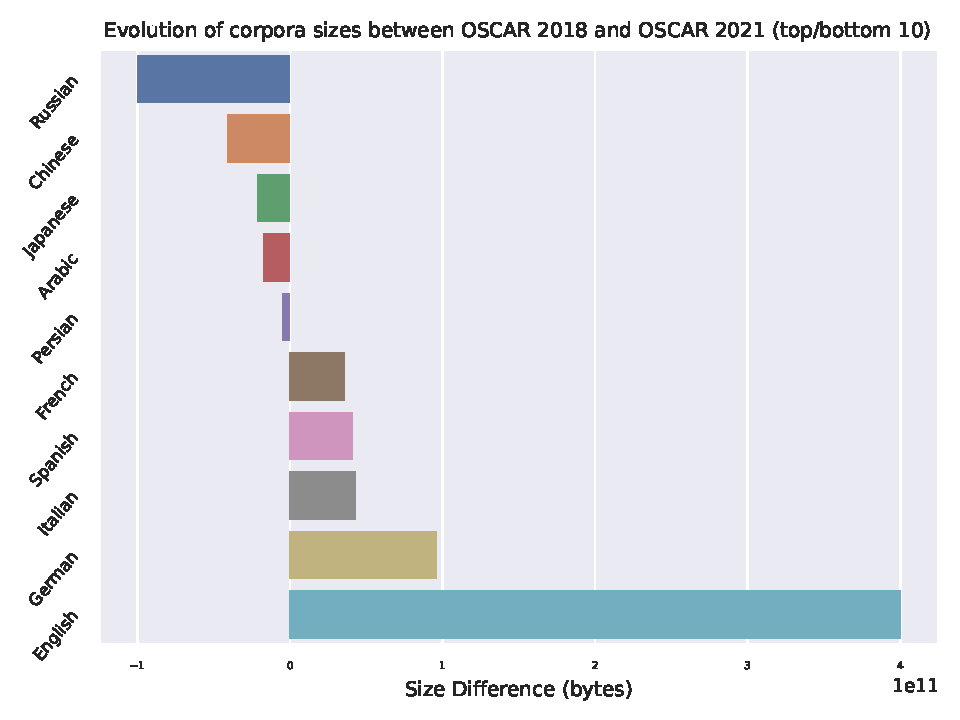
\includegraphics[width=0.75\textwidth, angle=0]{static/media/oscar/ungoliant/size_evo}
    \caption{Comparison of language size (in bytes) between OSCAR 2018 and OSCAR 2021 (top/bottom 5 only). }
    \label{fig:lang-size}
\end{figure}

Results show that already largely represented languages gain more and more data (like the English language, which constituted more than a third of the original OSCAR 2019), except for the Russian language which loses approximately 100Gb of textual content. These results are summarized in Figure~\ref{fig:lang-size}.

However, in a context where the number of languages is very high (higher than 150) and of varying sizes, evolution can't be analyzed via a mere size evaluation. By computing, for each language, the relative size difference between the 2019 and 21.09 releases of OSCAR, less resourced languages do appear, hinting at a better representation of some of them. These results can be found in Figure~\ref{fig:lang-size-pctg}.

Note nonetheless that numerous languages have been omitted from Figure~\ref{fig:lang-size-pctg}, either:
\begin{itemize}
    \item because they were present in the original OSCAR 2019 and are now absent (\textit{Central Bikol} and \textit{Cantonese})
    \item or because they were absent in the original OSCAR 2019 and are now present (\textit{Manx}, \textit{Rusyn}, \textit{Scots} and \textit{West Flemish})
\end{itemize}

Precautions have to be taken when using these corpora and further work has to be done to correctly assess the quality of low-to-mid resource languages in order to better reflect the quality of each corpus to the OSCAR users. Some sub-corpora exhibited either a particularly low number of sentences or just very low quality data, and as such they are not really usable in practice. However, they still account for a language in the total language count of both the original OSCAR 2019 and the new OSCAR 21.09.

\begin{figure}[ht]
    \centering
    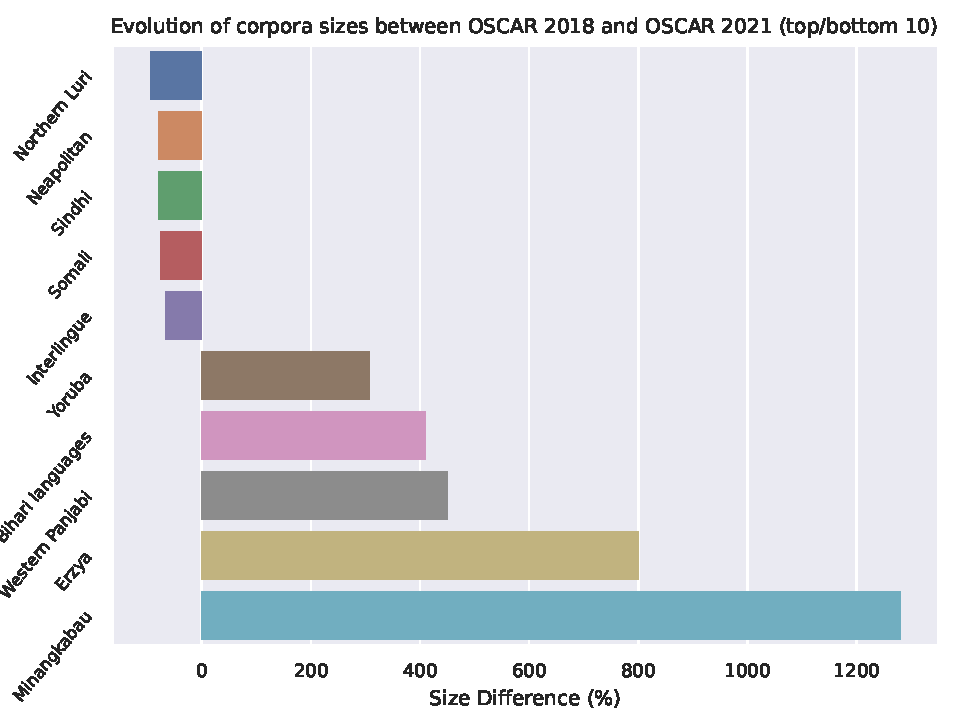
\includegraphics[width=0.75\textwidth, angle=0]{static/media/oscar/ungoliant/size_evo_pctg}
    \caption{Comparison of language percentage between OSCAR 2018 and OSCAR 2021 (top/bottom 5 only).}
    \label{fig:lang-size-pctg}
\end{figure}

\subsubsection{Metadata}

Metadata provides new contextual data that is useful to evaluate the corpus and draw metrics.

The total size of metadata is 1.2 TB, ranging from 4Kb to 500Gb, depending on the number of lines. Relative size varies from 100\% to 20\%, diminishing with the textual data size, which is expected.

Our choice of keeping metadata aside from the main content adds some complexity when working with both textual and contextual data:

\begin{itemize}
    \item When trying to get the metadata of given sentence, one has to get the line number $k$, then sequentially (or use a search algorithm since offsets are sorted) look for the record (with offset $o$ and length $l$), where $k \in [o, o+l]$.
    \item Looking for lines corresponding to a particular metadata entry is easier: one has to read the textual file, skipping until the $o$-th line, then read $l$ lines.
\end{itemize}


\subsubsection{Presence of events}

Using a sample of five sub-corpora, we perform a simple search of terms in order to assess and compare the presence of pre- and post- 2018 events and persons in both corpora. Terms and frequency are grouped in Table \ref{tab:word-frequency}.

\begin{table}[t]
    \centering\small
    \begin{tabular}{lrrrr}
        \toprule
        Language                  & Term                  & 2018  & 2021  \\
        \midrule
        \multirow{1}{*}{Arabic}   & Beirut port explosion & 0     & 31    \\
        \multirow{1}{*}{Burmese*} & Min Aung Hlaing       & 387   & 3439  \\
        \multirow{1}{*}{English}  & Obama                 & 30039 & 27639 \\
        \multirow{1}{*}{English}  & Biden                 & 990   & 19299 \\
        \multirow{1}{*}{French}   & Yellow Vests          & 2     & 96    \\
        \bottomrule
    \end{tabular}
    \caption{Comparison of occurrences of news-related terms between OSCAR and our corpus in a sample of 100 Common Crawl shards. For the Burmese language, we use the whole 2018 and 2021 corpus since it is a low resource language. Terms are translated to the target language.}
    \label{tab:word-frequency}
\end{table}

Our corpus keeps around the same number of occurrences for pre-2018 events or public figures such as Barack Obama, while increasing the occurrence of people linked to more recent events (Joe Biden).

We include search terms linked to post-2018 events in French and Arabic which are smaller corpora (resp. 200 and 80 GB), and in Burmese, a mid-resource language (approximately 2 GB). We observe a term occurrences evolution that reflects the linked events' timing and importance.

\subsection{License}

This new OSCAR 21.09 corpus is released under a research-only license that is compliant with the EU's exceptions for research in text and data mining. Contrarily to the original OSCAR 2019, no shuffled version of the corpus is distributed, instead we put in place an authentication system that allows us to verify that requests for the corpus come from research institutions. A contact form is also provided for independent researchers so that we can study their particular cases and determine if the utilization of the corpus corresponds to a legitimate research use.

Moreover, the introduction of metadata makes our corpus far more queryable, thus simplifying and speeding up the handling of take-down GDPR requests. For this reason, we release the complete set of metadata under a CC0 public domain license, so that any individual can check if their personal or even copyrighted data is in our new OSCAR 21.09 corpus and make a request accordingly.

\section{Conclusion}

Although the work presented in this particular chapter does not directly address some of the previous concerns raised by \citet{caswell-etal-2020-language,kreutzer-etal-2021-quality}. We do believe that a more efficient, more modular and better documented pipeline is the first step in making the OSCAR project more approachable by other members of the NLP and Digital Humanities communities.

Moreover, we also believe that the addition of metadata to OSCAR is a big step towards improving the quality of its content as it will provide us and other researchers willing to use OSCAR with enough information to better explore, audit, annotate and filter the corpus.

In the next and final chapter of the OSCAR part we will explore the question of document integrity which might be useful for researchers interested in document level tasks and which until now is not respected for Common Crawl records containing multilingual data. We will also continue improving Ungoliant and start using the metadata that we extract from the Common Crawl records to produce the first ever OSCAR annotations.
\chapter{Towards a Cleaner Document-Oriented Multilingual Crawled Corpus}

\section{Filtering}

Previous OSCAR pipelines were line-oriented (where a line is defined as a string separated by \texttt{\textbackslash n}), which meant that the highest filtering granularity were lines.
Having a document-oriented corpus implies that:
\begin{itemize}
    \item We must try to keep the document integrity, by altering it in a way that does not completely destroy its coherence.
    \item Operations on the document (filtering, identification, annotation) must take into account the document as a whole.
\end{itemize}

We aim to produce a corpus that is similar in size and quality to OSCAR 21.09, looking for a set of filters that limits the inclusion of short, noisy lines in documents, while keeping a sufficient quantity of data, especially for low- and mid-resource languages. Those filters either keep/discard a given document, or remove lines from the document body then keep it.

\subsection {Header and footer filter}

Similar to previous OSCAR pipelines, we use a length-based filter discarding short-lines. However, we restrict the removal on contiguous sequences of short lines that are located either at the head or at the tail of the document. In the following document, only the lines preceded by an exclamation point would be kept.

\begin{verbatim}
Home
Login
Sign Up
Welcome to my Website
! Lorem Ipsum Dolor Sit Amet ....
! Lorem Ipsum Dolor Sit Amet ....
! Lorem Ipsum Dolor Sit Amet ....
! Lorem Ipsum Dolor Sit Amet ....
Copyright Myself
Legal
Contact
\end{verbatim}

The solution still has numerous drawbacks, especially when dealing with documents crawled from the internet, a source known to be extremely noisy and full of edge cases: Adding a long line at the very head and tail of the previous document would completely negate the benefits of the filter.

\subsection{Short lines proportion filter}

In order to refine the filtering process, we use a count-based filter that separates the data in two bins: One for short lines and one for long lines. The filter then checks which bin is bigger, and filters out documents where the short lines bin is bigger.

This filter may limit the impact of documents containing low-quality long lines at the head/tail, then a high number of short lines.


\section{Identification}

The backbone of the language identification process is similar to the one used in goclassy \cite{ortiz-suarez-etal-2019-asynchronous} for the generation of OSCAR 2019 and Ungoliant \cite{abadji-etal-2021-ungoliant} for the generation of OSCAR 21.09. However, shifting to a document oriented corpus (with a single top-level identification per document) requires to infer the document identification, based on line identifications.


We define a document $\mathcal{D}$ as a pair $\mathcal{D}=(\mathcal{L}, \mathscr{L})$ where $\mathcal{L}=\{l_1,\ldots,l_n\}$ is the set of lines (strings separated by \texttt{\textbackslash n}) that constitute the document and $\mathscr{L} = \{g_1, \ldots, g_m\}$\footnote{Note that since FastText identifies one language by line, we have always have $m\le n$ for every document $\mathcal{D}$.} is the set of languages identified by FastText for the document $\mathcal{D}$. When FastText is no able to identify a language for an specific line, for instance because the confidence isn't higher than $0.8$, we tag said line with the \emph{No Identification Language} that we simply note by $g_0$. Furthermore, we define each line $l_i$ in a document $\mathcal{D}$ as a triplet $l_k=(g_i, p_i, s_i)$ where $g_i$ is the language identified by FastText with the highest confidence for the line $l_i$, $p_i$ is said confidence and $s_i$ is the size in bytes of the line $l_i$. We also note $|l_i|=s_i$ and we thus define the size $|\mathcal{D}|$ of a document $\mathcal{D}$ as
\[
    |\mathcal{D}| = \sum_{i=0}^{n} |l_i| = \sum_{i=0}^{n} s_i.
\]
Moreover, for each identified language $g_j \in \mathscr{L}$ in a document containing $n$ lines, we define its size $|g_j|$ as
\[
    |g_j| = \sum_{\mathclap{\{s_i \mid g_i = g_j\}}} s_i.
\]
Finally for each language $g_j \in \mathscr{L}$ we can also compute its \emph{overall weighted confidence} $P_j$ throughout the document $\mathcal{D}$ as the following weighted mean:
\[
    |P_j| = |D|^{-1}\sum_{\mathclap{\{s_i|g_i=g_j\}}} s_jp_j.
\]

\subsection{Multilingual document identification}

A document can contain lines in multiple languages for several reasons:
\begin{enumerate}
    \item Identification mismatch, that can show up frequently, especially with languages that have significant vocabulary overlap (Czech and Slovak),
    \item Crawl from a website where the interface is written in a language, and the body is written in another one,
    \item Crawl from a translation page, where the same content is present in two (or more) different languages.
\end{enumerate}

In these examples, we should aim to limit the presence of 1. and 2., while maximizing the presence of 3.: documents having a balanced set of lines per language. Thus, we decide to take a cautious approach, restricting the multilingual document identification test to the documents that:
\begin{itemize}
    \item Have at least $5$ lines,
    \item Have at most $5$ different languages.
\end{itemize}
Next, we compute the \emph{proportion} for each language $g_j \in \mathscr{L}$ in the document $\mathcal{D}$ defined as follows
\[
    \mathrm{Pr}_g = \frac{|g|}{|\mathcal{D}|},
\]
including for the no identification language $g_0$.

A document $\mathcal{D}$ containing $n$ lines is identified as multilingual if and only if:
\[
    \begin{dcases}
        |g_j| \ge \frac{|\mathcal{D}|}{n+1} & \forall g_j \neq g_0, \text{and} \\
        |g_0| \le \frac{|\mathcal{D}|}{n+1}
    \end{dcases}
\]
As an example, a document holding $m=3$ languages is multilingual if each language makes up at least $\frac{1}{m+1} = \frac{1}{4}$ of the document, and that there is at most $\frac{1}{4}$ of the document that is of unknown identification.

\subsection{Monolingual identification}
We begin by identifying each line, keeping in memory the language identified, the confidence of the identification, and the size of the line. We keep track of lines that have not been identified with a special token, and a confidence of 1.

% For a document $D$ composed of $n$ sentences $\{s_1,\ldots, s_n\}$, we map each sentence $s_k$ with its identification $L_k$, confidence $p_k$ and size $|s_k|$. 
% \[
%     s_k \longrightarrow (L_k, p_k, |s_k|)
% \]
% Then, for each language $L_x$ present in the document, we compute the size
% \[
%     |L_x|=\sum_{\mathclap{\{s_k|L_k=L_x\}}} |s_k|
% \]
If the document does not pass the multilingual check, we then take the largest represented language and compute its overall confidence $P_j$ and use a minimum confidence threshold of $0.6$ that is way lower than the previous pipelines ($0.8$). This is motivated by the following reason: The document-based filtering removes documents containing lines that could have been kept by former pipelines, thus reducing the size of the generated data.

Using a lower threshold could help getting lower-quality documents that still hold high-confidence lines in themselves.

\section{Annotation}

While the filtering and identification steps are lenient by using lower thresholds than the previous pipelines, we introduce annotations, as non-destructive filters that enable more precise downstream filtering for the corpus users, as well as a useful resource to quickly assess the quality of a corpus. Annotations enable more aggressive filters to be run, since the non-destructive nature of annotations can in turn be used to refine annotation filters.

Numerous annotations are available, and each document can have several ones at the same time.

\subsection{Length-based annotations}

Some simple annotations are added when documents doesn't meet certain length requirements:

\begin{itemize}
    \item The document has a low ($\le 5$) number of lines (\emph{tiny})
    \item The document has a high number ($\ge 50\%$) of short lines (\emph{short\_sentences})
\end{itemize}

These annotations helps spotting potentially tiny documents, where the line structure or the document size could negatively influence training tasks.

A third annotation checks the occurrence of short lines at the start of the document, and adds a \emph{header} annotation if it is the case, indicating that low-quality content could be present at the start of the document.

A fourth annotation named \emph{footer} works in the same way on the tail of the document.

\subsection{Noise detection}

Some documents make their way into the corpus while being extremely noisy or non-linguistic. As an example, source code can be found in English corpora because of the presence of English words in the source itself.

We use a filter that computes a ratio between letters and non-letters.

This filter is based on Unicode categories. We use categories \emph{Lu, Ll, Lt, Lm, Lo}\footnote{Lu: Uppercase letter, Ll: Lowercase letter, Lt: Titlecase, Lm: Modifier, Lo: Other} for letters, and we add categories \emph{Mn, Mc, Me}\footnote{Mn: Nonspacing mark, Ms: Spacing mark, Me: Enclosing mark} for accents and diacritics.

A \emph{noisy} annotation is added if the ratio passes a certain threshold, set to $0.5$.


\subsection{Adult documents}

We use the UT1 blocklist\footnote{\url{https://dsi.ut-capitole.fr/blacklists/}} as a base for adult content filtering.

The UT1 blocklist is a collection of thematic blocklists (adult, gambling, blogs, ...), usually utilized in internet access control for schools. The list is constituted and extended by both human and robots contributions (known indexes, search engines, exploration of already known addresses). The blocklist is updated twice to thrice a week by Fabrice Prigent.

Each folder contains URL and domain blocklists, enabling filtering of both websites that are centered around adult content, and websites hosting user-generated content that can be of adult nature (several social networks...).

The adult blocklist is comprised of roughly 3.7M records.

%By matching on document URL both on domain and URL blocklists, we get between 10-20 annotated documents per shard (a shard = ~10k documents).

%By matching on document URL on a corpus sample, we notice some recurring false positives: 
%\begin{itemize}
%    \item Sane material that may have been misclassified (sports blogs, review sites..),
%    \item Sane material that is wrongly flagged as adult but contains non-adult LGBTQI+ content (one of the main french gay magazines is present in the blocklist)
%\end{itemize}

%Even if we can't guarantee an absence of false positives/false negatives, we can do better, since tetu.fr is a news site with high quality documents for example.

%We could: 

%\begin{itemize}
%    \item use a ngram that recognizes adult content on documents body and fetch URLs where %this type of content is prevalent, thus building a "custom" blocklist 
%    \item train an ngram model on documents that have been annotated as adult, then use this %ngram model to filter content. (if we use some filtering we may be able to avoid %categorising sports/LGBTQI+ content as adult).
%\end{itemize}
%The sanity of the documents that haven't been annotated has to be assessed.

%The usage of a simple (but applicable) ngram-based model has to be assessed. (On the URLs AND on the content!)


\section{Corpus}

We apply the aforementioned pipeline to the November/December 2021 crawl dump of CommonCrawl. The result is a new corpus, OSCAR 22.01. While its structure is different from the previous OSCAR corpora (due to the choice of generating a document oriented corpus), we attempt to compare the two corpora, especially in terms of size and news-related topic presence and recall. We also evaluate the occurrence and pertinence of the annotations.

\subsection{Comparison with OSCAR 21.09}
\subsubsection{Size distribution}

The data layout of OSCAR 22.01 may limit the relevance of raw size comparisons, since metadata are larger (annotations and line identifications were not present in previous OSCAR Corpora), and fused with textual data (metadata were distributed in separate files for OSCAR 21.09).

However, comparing the distribution of corpus sizes may help us ensure that the new corpus has a size distribution similar to the older one.

We compare the distribution of the corpus sizes between OSCAR 21.09 and OSCAR 22.01 in figure \ref{fig.1}. We see that while the overall distribution is similar, the lower end of the distribution has more variance: The $[0\text{B}, 100\text{KB})$ range shows more corpora at its bounds than at its center. We also plot the empirical cumulative density function, that helps to assert the distribution similarity between OSCAR 21.09 and OSCAR 22.01.

\begin{figure*}[!ht]
    \begin{center}
        %\fbox{\parbox{6cm}{
        %This is a figure with a caption.}}
        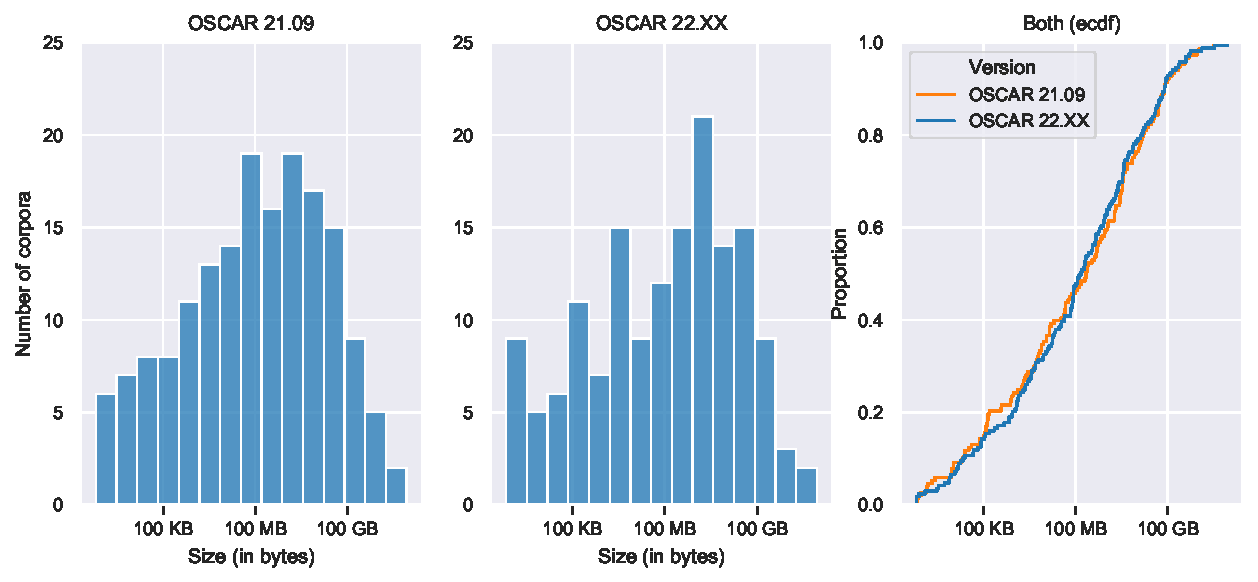
\includegraphics[scale=0.7]{static/media/oscar/towards/size-comp}
        \caption{Corpus size distribution between OSCAR 21.09 and 22.01}
        \label{fig.1}
    \end{center}
\end{figure*}

We also select three low-resourced languages, three mid-resourced languages and three high-resources languages and compare their content (that is, textual data excluding metadata) between OSCAR 22.01 and OSCAR 21.09. Comparison is shown in figure \ref{fig.2}. While the overall sizes of these corpora  have slightly decreased, the sizes of the mid and high resource languages are similar enough.

\begin{figure}[!ht]
    \begin{center}
        %\fbox{\parbox{6cm}{
        %This is a figure with a caption.}}
        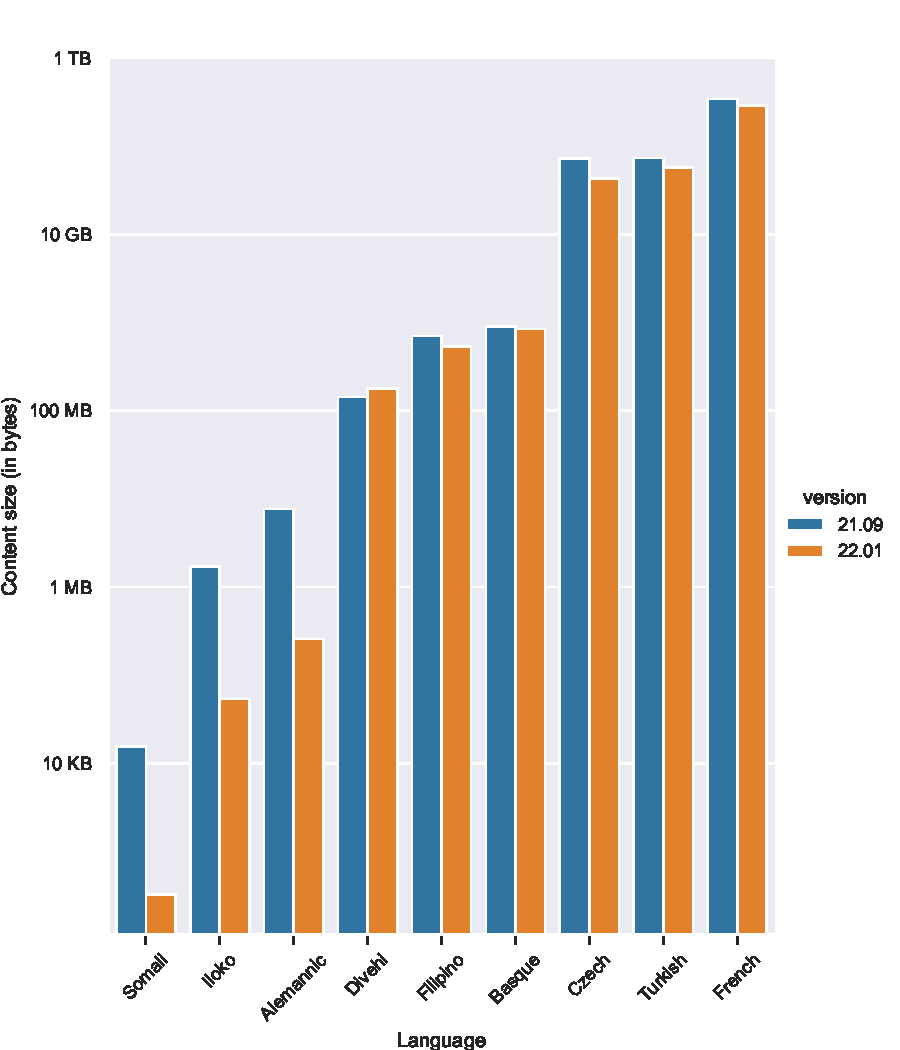
\includegraphics[width=\linewidth]{static/media/oscar/towards/size_comp_content}
        \caption{Content size comparison of selected languages in OSCAR 22.01 versus OSCAR 21.09}
        \label{fig.2}
    \end{center}
\end{figure}

\subsubsection{Size differences in low-resource languages}

The low-sized corpora exhibit important size changes. As an example, the Alemannic German corpus went from 7MB to 360KB between OSCAR 21.09 and OSCAR 22.01. This size decrease can be explained by the way the document identification works: by reasoning at a document level, documents containing a majority of German identified lines and a minority of Alemannic German identified lines will be identified as a German document, whereas previous OSCAR pipelines would have separated the lines and increase the size of the Alemannic German corpus.

By extracting the lines identified as Alemannic from the German corpus, we get around 30 MB of data, which could constitute an Alemanic corpus with a size comparable to the OSCAR 21.09 Alemanic corpus after confidence and length based filterings.


This situation can, in a way, help us investigate the cases of linguistic proximity, where languages have a lexical overlap: When a line identified as Alemannic German is found inside a document that has been identified as German:
\begin{enumerate}
    \item \label{one} Is the line in German and it is an identification error?
    \item Is the line in Alemannic German, in a document that is in German? (ex: A German website related to the Alemannic German language)
    \item \label{three} Is the whole document in Alemannic German, and the identification classified the majority of Alemannic as German?
\end{enumerate}

Those three cases can arise and may help to enhance the detection of a said language, by finding (\ref{one}) identification mismatches, hoping that these cases would improve identification after training, or (\ref{three}), after verification by a speaker of the language, state that the whole document is in Alemannic. The new data collected could in turn be used to improve language detection.


\subsubsection{New themes}

As OSCAR 22.01 is based on a November/December 2021 dump (compared to OSCAR 21.09, based on a February 2021 dump), the corpus should include data related to events contemporary to February 2021. We conduct a simple word search similar to the one conducted for the generation of OSCAR 21.09 \cite{abadji-etal-2021-ungoliant}, using both old and new events, in order to give a rough idea of both the actuality and the memory of the corpus.

\begin{table}[t]
    \centering\small
    \begin{tabular}{lrrrr}
        \toprule
        Language                  & Term                  & 21.09 & 22.01 \\
        \midrule
        \multirow{1}{*}{Arabic}   & Beirut port explosion & 31    & 13    \\
        \multirow{1}{*}{Burmese*} & Min Aung Hlaing       & 3439  & 2736  \\
        \multirow{1}{*}{English}  & Obama                 & 27639 & 8697  \\
        \multirow{1}{*}{English}  & Biden                 & 19299 & 8232  \\
        \multirow{1}{*}{English}  & Omicron               & 131   & 417   \\
        \multirow{1}{*}{French}   & Yellow Vests          & 96    & 73    \\
        \multirow{1}{*}{Spanish}  & Aborto                & 1504  & 572   \\
        \bottomrule
    \end{tabular}
    \caption{Comparison of occurrences of news-related terms between OSCAR and our corpus in a sample of 100 CommonCrawl shards. \\ *: For the Burmese language, we use the whole 21.09 and 22.01 corpus since it is a low resource language. Terms are translated in the corpus language.}
    \label{tab:word_frequency_towards}
\end{table}

We see that the events and terms related to events predating February 2021 are still occurrent in the corpus, but have a diminished count that is in the same order of magnitude.
We also count the occurrences of the term Omicron, related to the Omicron variant, and observe that the term has a higher count on the 21.09 sample.

\subsubsection{Absence of deduplication}

Contrary to OSCAR 21.09, we do not distribute a deduplicated version of the majority of OSCAR 22.01.

The line-level deduplication of documents would have destroyed the integrity of documents themselves, hampering human readability and even sequential sentence sense. We can imagine having forum discussions' sense destroyed because of identical responses, or song lyrics being altered.

Moreover, the similarity-based document-level deduplication procedure is very costly in terms of computing power and time \cite{gao-etal-2020-pile}.

We make the choice of distributing a non deduplicated version of OSCAR along with a deduplicated, line oriented version of the English corpus, while encouraging the use of deduplication in the context of training language models \cite{lee-etal-2021-deduplicating}.
A line-level deduplication tool will be available as part of the OSCAR toolkit\footnote{\url{https://github.com/oscar-corpus/oscar-tools}}. We will also distribute a deduplicated version of the English part of OSCAR 22.01, with a data layout similar to OSCAR 21.09 corpora.


\subsection{Annotations}

\subsubsection{Raw stats}

Annotations helps us to infer the composition of the corpora: The \textit{tiny}, \textit{short\_sentences} and especially \textit{noisy} annotations may indicate documents of a varying poor quality, with \textit{noisy} being the worst.

Also, comparing corpora annotation distributions, especially related to their size, could highlight potentially very low quality corpora. This semi-automated quality checking process could be used to label corpora where data quality is bad.

We select 3 low-resource ($\simeq100KB$), 3 mid-resource ($\simeq100MB$) and 3 high-resource ($\simeq100GB$) languages and plot the number of documents per annotation, adding a \textit{total} legend for the total document count and a \textit{clean} legend for documents that do not have any annotation. We then plot the counts for each resource group using adapted scales.

We observe that the annotation distribution is similar for each resource group, but that the lower resourced languages have a higher proportion of documents annotated with \textit{short\_sentences} and \textit{tiny}.

\begin{figure*}[!ht]
    \begin{center}
        %\fbox{\parbox{6cm}{
        %This is a figure with a caption.}}
        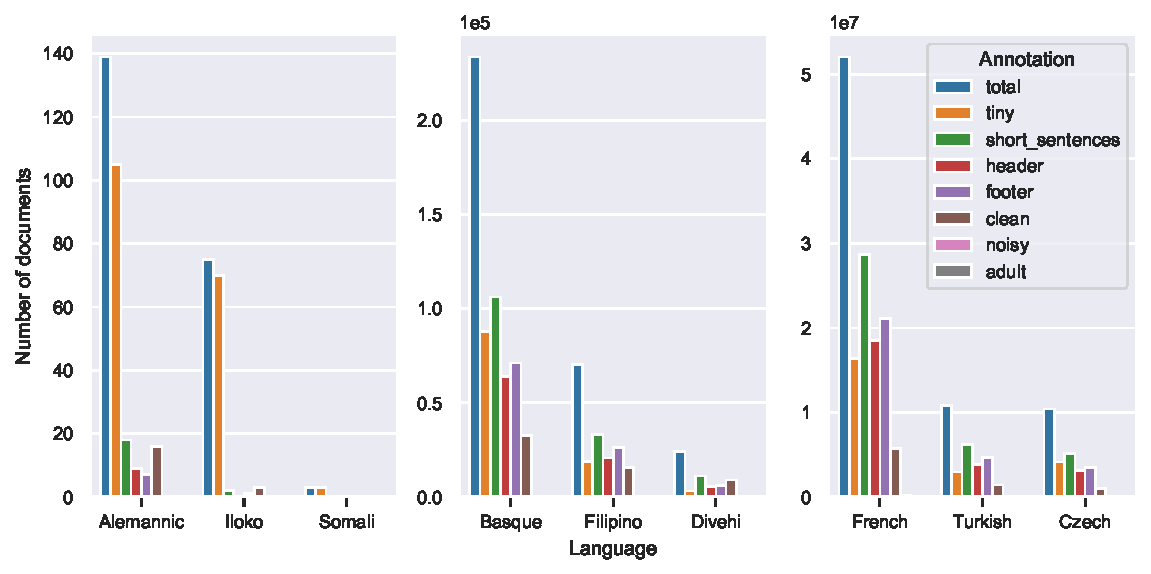
\includegraphics[scale=0.7]{static/media/oscar/towards/annot_count.pdf}
        \caption{Annotation count in selected low, mid and high resource languages (scales are adapted to corpus size)}
        \label{annot-count}
    \end{center}
\end{figure*}

In order to better compare the resource groups, we display the annotation distribution in a heat map (figure \ref{annot-heatmap}).
We notice important differences between low and mid/high resource groups.
A very large proportion of the low resource group is annotated as \textit{tiny} while simultaneously detaining few documents annotated \textit{short\_sentences}, indicating the presence of long sentences within documents with a low number of sentences.

\begin{figure}[!ht]
    \begin{center}
        %\fbox{\parbox{6cm}{
        %This is a figure with a caption.}}
        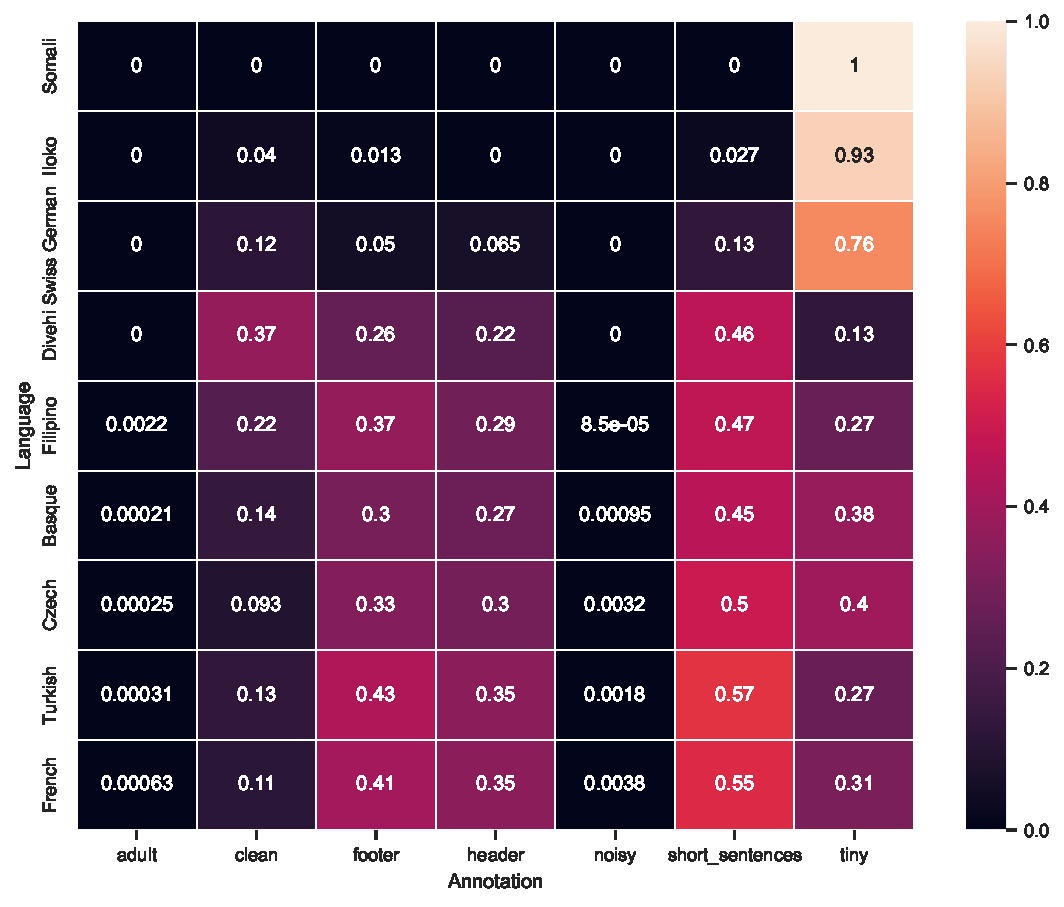
\includegraphics[width=\linewidth]{static/media/oscar/towards/annot_heatmap}
        \caption{Heat map of annotation distributions in selected low, mid and high resource languages.}
        \label{annot-heatmap}
    \end{center}
\end{figure}

\subsubsection{Multilinguality}

The OSCAR 22.01 Corpus also contains a multilingual corpus, composed of documents holding lines in multiple languages. Each document contains at least 2 languages, and at most 5.

We check the co-occurrence of languages, highlighting the coupling of language tuples. These tuples may highlight either linguistic similarity (Czech and Slovak, Russian and Uzbek) and subsequent poor classification, errors or languages commonly found together on documents. Due to the number of languages and the sparsity of the data, we show the language couples with a number of documents greater than 20 000 (Figure \ref{multi-confusion}).

We also note the presence of English in a high number of documents. This could be explained by boilerplate content in web pages, such as menu headers or footers.


\begin{figure}[!ht]
    \begin{center}
        %\fbox{\parbox{6cm}{
        %This is a figure with a caption.}}
        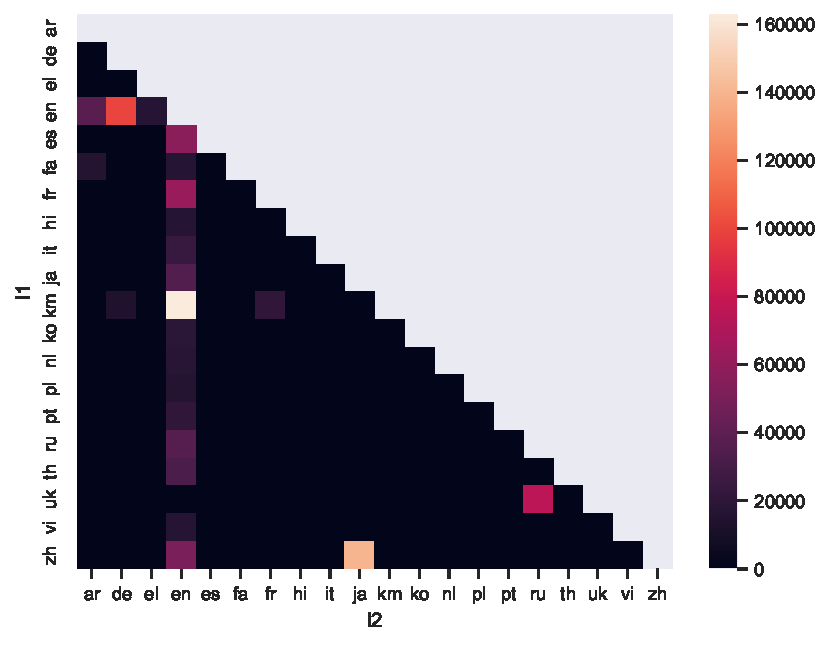
\includegraphics[width=0.8\linewidth]{static/media/oscar/towards/multilingual_big}
        \caption{Count of $(l1, l2)$ language tuples in the multilingual corpus. Languages tuples with less than 20,000 occurrences are not shown.}
        \label{multi-confusion}
    \end{center}
\end{figure}

Using the clean annotation filter on the multilingual corpus may help to retrieve the highest quality multilingual documents.

\subsubsection{Clean documents}

We also look into documents that did not get annotated at all, and we find that these documents are usually of a high quality. However, their relative proportion in corpora may limit their usage.

We use a sample of the English corpus (183,497 documents, 1.3 GB) and compare the size of documents depending on the presence (or not) of annotations. The stacked counts are shown in figure \ref{clean_count}.

We observe that clean document mean length is slightly shorter than non-clean ones. Also, we note that while the length standard deviation of clean documents seems to be shorter, the computation yields larger numbers, caused by outliers in the high end (Annotations: $\mu=8606$ $\sigma=49874$, Clean: $\mu=6537$ $\sigma=14983$).
By removing the top and bottom 5\%, we get (Annotations: $\mu=3686$ $\sigma=4047$, Clean: $\mu=3582$ $\sigma=3202$).

These results are not sufficient to state on the intrinsic quality of the clean documents, but may ease the study of the filters and identify future filtering needs.

\begin{figure}[!ht]
    \begin{center}
        %\fbox{\parbox{6cm}{
        %This is a figure with a caption.}}
        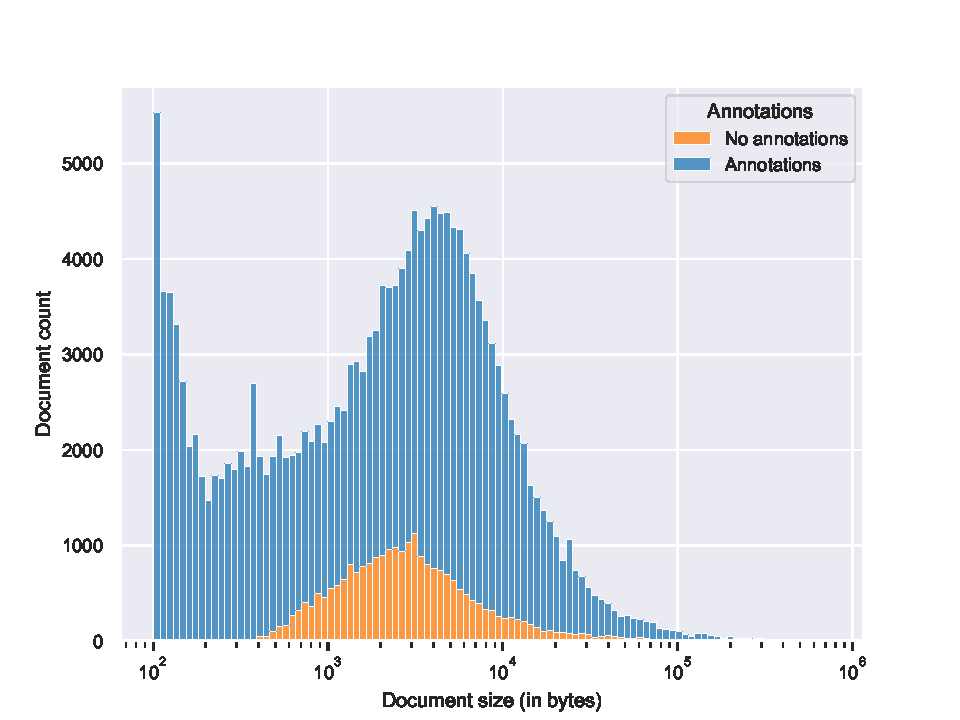
\includegraphics[width=\linewidth]{static/media/oscar/towards/num_doc_clean}
        \caption{Stacked distribution of annotated and non-annotated (clean) documents on a selection of the English corpus}
        \label{clean_count}
    \end{center}
\end{figure}

\subsubsection{Adult documents}

While very small in proportions, adult annotation documents highlight interesting facts.

The French sample contains 32,870 adult documents, out of 52,037,098.

We count if some documents coming from tetu.com are labeled as adult, in order to probe the possibility of finding LGBTQI+ content annotated as adult. We find 1063 documents, representing $\sim 3.2\%$ of the adult documents. This may imply that more LGBTQI+ content sites are present in the blocklist, thus increasing the ratio of LGBTQI+ content labeled as adult.

We take the first 100 adult documents of the French corpus and check whether they are properly classified.
\begin{itemize}
    \item \emph{true positives} documents that exhibit explicit sexual content geared towards pornography (pornographic websites, sexually explicit fictions)
    \item \emph{false positives} documents that do not meet this criteria,
\end{itemize}

We separately count websites that are simultaneously non explicit and from LGBTQI+ websites.

We find:
\begin{itemize}
    \item $77$ true positives,
    \item $2$ false positives belonging to LGBTQI+ websites,
    \item $21$ false positives
\end{itemize}

While the majority of true positives are properly classified, numerous educational documents do appear: These type of documents exhibit an explicit language, but does feature a good document quality, and a better representation of sexuality that is less offensive compared to the usual associations between sexually explicit content and hate speech.  \cite{luccioni-viviano-2021-whats}.

The false positives are, for the majority, websites that do not belong in the blocklist in the first place. We suppose that the addresses were previously used as adult websites.


%Even if we can't guarantee an absence of false positives/false negatives, we can do better, since tetu.fr is a news site with high quality documents for example.

%We could: 

%\begin{itemize}
%    \item use a ngram that recognizes adult content on documents body and fetch URLs where %this type of content is prevalent, thus building a "custom" blocklist 
%    \item train an ngram model on documents that have been annotated as adult, then use this %ngram model to filter content. (if we use some filtering we may be able to avoid %categorising sports/LGBTQI+ content as adult).
%\end{itemize}
%The sanity of the documents that haven't been annotated has to be assessed.

%The usage of a simple (but applicable) ngram-based model has to be assessed. (On the URLs AND on the content!)

\subsubsection{Hard bounds problems}

Several pipeline steps (especially annotators), work using hard thresholds. As an example, any document that is less than 5 lines is considered to be \textit{tiny}. However, when exploring data, we can see that there is a number of documents whose number of lines is in the neighboring of the threshold, and quality is similar to the documents labeled as \textit{tiny}.

When plotting the distribution of clean and annotated corpus data, we can notice that a very high number of documents are of a tiny ($10^2 B$) size, which coincidentally happens to be the minimum size for a document to be accepted, since the first filter removes lines that are shorter than 100 characters $(\geq 10^2 B)$.


\section{Discussion}


\subsection{Corpus}
We provide a new, document-oriented corpus of the same size of OSCAR 21.09 that keeps document integrity and is easier to filter thanks to annotations.

While the mid and high resourced languages are of a similar size, several low resource languages have seen an important decrease of size.
We still have to check whether this size decrease comes with a quality increase, since previous low resource OSCAR corpora sometimes exhibited extremely poor quality: Many non-linguistic corpora that were published and deemed unusable weeks or months after release.

We also note that documents of similar languages could have been merged into larger corpora, and we show that the German corpus holds $\sim 30$MB of Alemannic that, with appropriate filtering, could be treated as an independent corpus. These cases of merging are also interesting to investigate, as they can explain identification mismatches and could, in turn, help to build better language identification models.
More work has to be done in order to properly map the connection between low-resource languages and mid and high resource languages potentially containing data in these languages.

\subsection{Annotations}

The selected annotations exhibit numerous caveats that have to be addressed in the future iterations of OSCAR generation pipelines.

The length-based annotations are widespread in the corpus, especially in mid to high resource languages ($\sim50\%$ in Czech) highlighting the potential low quality of a high number of documents as well as the need of better characterizing the nature of these line length discrepancies. Web crawls often contain boilerplate content extracted from headers, footers and sidebars, and these lines are present in the Common Crawl dumps.
Another solution would be to base the whole OSCAR generation pipeline on raw HTML files, potentially multiplying the computational cost and complexity of generating corpora.

The \textit{adult} annotation, based from an adult URL blocklist, is present on a very limited set of documents. However, studies have shown that adult content has been present in a previous version of OSCAR in a larger proportion than the one measured here \cite{kreutzer-etal-2021-quality}, hinting at a bad performance of the blocklist based adult content filtering approach. Moreover, we noticed that the blocklist contained websites representing LGBTQI+ related topics, which damages the representation of the LGBTQI+ (association with adult content, filtering out LGBTQI+ documents, which in turn could limit the representation in downstream tasks..).
Model-based approaches may help in improving the \textit{adult} annotation, and should be the next step towards a better annotation of adult content \cite{luccioni-viviano-2021-whats}.



\part{French Data}
\chapter{CaBeRnet: A Contemporary French Balanced Corpus}


\section{Corpora Building}%- Quantitative Description
\label{sec:DescribeCorpora}
%Two main criteria guided corpus building, the first was balance and representativeness, and the second was maximizing the usage of open resources to build our corpora.

\subsection{\Cabernet} \label{subsec:DescribeCaBeRnet}

\Cabernet corpus was inspired by the genre partition of the American balanced corpus COCA, %\footnote{\url{https://www.corpusdata.org}}
which currently contains over 618 million words of text (20 million words each year 1990-2019) and is equally divided among spoken, fiction, popular magazines, newspapers, and academic texts \citep{davies-2009-the, davies-2010-the}. A second reference, guiding our approach and sampling method, is one of the earliest precursors of balanced reference corpora: the BNC \citep{bnc-2007-the}, first covered a wide variety of genres, with the intention to be a representative sample of spoken and written language.

\Cabernet was obtained by compiling existing data-sets and web-text extracted from different sources as detailed in this section. As shown in Table \ref{Table_Morpho_CabernetSub}, genres sources are evenly divided ($\sim$120 million words each) into spoken, fiction, magazine, newspaper, academic to achieve genre-balanced between oral and written modality in newspapers or popular written style, technical reports and Wikipedia entries, fiction, literature or academic production).
%(cf. Metadata)
%Encompassing five different genres and registers : xxx

\paragraph{\Cabernet Oral} \label{subsec:DescribeCaBeRnetOral}
The oral sub-portion gathers both oral transcriptions (\textsc{ORFEO} and Rhapsodie\footnote{\textsc{ORFEO} corpus available at \url{www.cocoon.huma-num.fr/exist/crdo/} ; Rhapsodie corpus at \url{www.projet-rhapsodie.fr}.}) and Films subtitles (Open Subtitles.org), pruned from diacritics, interlocutors tagging and time stamps. To these transcriptions, the French European Parliament Proceedings (1996-2011), as presented in \citet{koehn-2005-europarl}, contributed a sample of more complex oral style with longer sentences and richer vocabulary.%\url{www.opensubtitles.org/fr}

\paragraph{\Cabernet Popular Press} \label{subsec:DescribeCaBeRnetPop}
The whole sub-portion of Popular Press is gathered from an open data-set from the \textit{Est  Républicain} (1999, 2002 and 2003), a regional press format\footnote{Corpus available at \url{www.cnrtl.fr/corpus/estrepublicain/}.}. %Ce corpus est constitué des données textuelles correspondant à deux années de toutes les éditions intégrales du quotidien régional.
It was selected to match popular style as it is characterized by easy-to-read press style and a wide range of every-day topics characterizing local regional press.

\paragraph{\Cabernet Fiction \& Literature} \label{subsec:DescribeCaBeRnetFic}
The Fiction \& Literature sub-portion was compiled from march 2019's Wiki Source and WikiBooks dump and extracted using WikiExtractor.py, a script that extracts and cleans text from a WikiMedia database dumps, by performing template expansion and preprocessing of template definitions.\footnote{Script available at \url{https://github.com/attardi/wikiextractor}.}

\paragraph{\Cabernet News} \label{subsec:DescribeCaBeRnetNews}
The News sub-portion builds upon web crawled elements, including Wikimedia's NewsComments and WikiNews reports from may 2019 WikiMedia dump, collected with a custom version of WikiExtractor.py.
Newspaper's content gathered by the Chambers-Rostand Corpus (i.e. Le Monde 2002-2003, La Dépèche 2002-2003, L'Humanité 2002-2003) and \textit{Le Monde diplomatique} open-source corpus were assembled to represent a higher register of written news style from different political and thematic horizons.
Several months of French Press Agency reports (AFP, 2007-2011-2012) competed with more simple and telegraphic style the newspaper written sample of the corpus.\footnote{At the time being, this part of \Cabernet corpus is still subject to Licence restrictions. This restricted amount of AFP news reports can reasonably fall in the public domain.}

\paragraph{\Cabernet Academic} \label{subsec:DescribeCaBeRnetAcad}
The academic genre was also built from different sources including technical and educational texts from WikiBooks and Wikipedia dump (prior to 2016) for their thematic variety of highly specialized written production. \textsc{ORFEO} Corpus offered a small sample of academic writings like PHD dissertations and scientific articles encompassing a wide choice of disciplinary topics, and TALN Corpus\footnote{TALN proceedings corpus (about 2 million) builds on a subset of 586 scientific articles (from 2007 to 2013), namely TALN and RECITAL. Available at \url{redac.univ-tlse2.fr/corpus/taln_en.html}.} was included to represent more concise written style characterizing scientific abstracts and proceedings.

\begin{table}[ht]
    \centering\small
        \begin{tabular}{lrrr}                                                                                      \\\toprule
            {\textsc{\Cabernet Sub-set}} & {\textsc{Tokens}} & {\textsc{Unique Forms}} & {\textsc{TTR}} \\\midrule
            Oral                         & 122 864 888       & 291 744                 & 0.0024         \\
            Popular                      & 131 444 017       & 458 521                 & 0.0035         \\
            News                         & 132 708 943       & 462 971                 & 0.0035         \\
            Fiction                      & 198 343 802       & 983 195                 & 0.0050         \\
            Academic                     & 126 431 211       & 1 433 663               & 0.0113         \\
            \textit{Total}               & 711 792 861       & 2 558 513               & 0.0036         \\ \bottomrule
        \end{tabular}
    \caption{\label{Table_Morpho_CabernetSub} Comparison of number of unique forms in the different genres represented by \Cabernet partition. TTR: Type-Token Ration. Lemmatization and tokenization was performed as described in §\ref{sec:CompareCorpora}.}
\end{table}
%%%check !! 
%\begin{table}[htbp]
%\centering
%\scalebox{0.83}{
%\begin{tabular}{lrrr}\\
%\toprule
%\multicolumn{2}{}{French Balanced Reference Corpus - \textbf{\Cabernet}}\\\midrule
%{\sc \textbf{\Cabernet}}   & nb{\sc Tokens}    & nb {\sc Unique Forms}  & Mo \\\midrule
%Oral        &  122,864,888      & 291,744  & 735,4 Mo   \\ 
%Popular     &  131,444,017      & 458,521  & 758,5 Mo   \\  
%News        &  132,708,943      & 462,971  & 797,2 Mo   \\ 
%Fiction     &  198,343,802      & 983,195  & 1 080 Mo    \\
%Academic    &  126,431,211      & 1433663  & 810,8 Mo   \\
%Tot.        &  711,792,861     & 2,558,513 & 4 190 Mo   \\ \bottomrule  
%\end{tabular}}
%\caption{\label{Table_TTR_CabernetSub} Comparison of number of unique forms in the different genres represent by \Cabernet partition into Oral, Popular, News, Fiction and Academic. Mo: Mega Octet. lemmatisation and tokenisation was achieved as described in section \ref{sec:CompareCorpora}}
%\end{table}
%voir si remplaçabl

For all sub-portions of \Cabernet, visual inspection was performed to remove section titles, redundant meta-information linked to publishing schemes of each of the six news editor includes. This was manually achieved by compiling a rich set of regular expressions specific of each textual source to obtain clean plain text as an outcome.


\subsection{French Children Book Test (CBT-fr)}
\label{subsec:DescribeCBT}

The French Children Book Test (CBT-fr) was built upon its original English version, the Children Book Test (CBT) \citet{hill-etal-2016-the}\footnote{This data-set can be found at \url{www.fb.ai/babi/}.}, which consists of books freely available on \url{www.gutenberg.org}{Project Gutenberg}.

Using youth literature and children books guarantees a clear narrative structure, and a large amount of dialogues, which enrich with oral register the literary style of this corpus.
The English version of this corpus was originally built as benchmark data-set to test how well language models capture meaning in context. It contains 108 books, and a vocabulary size of 53,628.

French version of CBT, named CBT-fr, was constructed to guarantee enough linguistic similarities between the collected books in the two languages. 104 freely available books were included. One third of the books were purposely chosen because they were classical translations of English literary classics. % (see Metadata). %www.cabernet-corpus.fr 
Chapter heads, titles, notes and all types of editorial information were removed to obtain a plain narrative text. The effort of keeping proportion, genre, domain, and time as equal as possible yields a multilingual set of comparable corpora with a similar balance and representativeness.

\begin{table}[ht]
    \centering\small
        \begin{tabular}{lr}                                                             \\\toprule
            {\textsc{Children Book Test - fr}}           & { \textsc{words}} \\\midrule
            number of different lemmas                   & 25 139            \\
            total number of forms                        & 95 058            \\
            mean number of forms per lemma               & 3.78              \\
            Number of lemmas having more than one form : & 14 128            \\
            Percentage of lemmas with multiple forms     & 56.20             \\
            \bottomrule
        \end{tabular}
    \caption{\label{Table_DescribeCBTfr} Lexical statistics of French CBT, performed as described in §\ref{sec:CompareCorpora}}
\end{table}

%%%%%%%%%%%%%%%%%%%%%%%%%%%%%%%%%%%%%%%%%%%%%%%%%%%%%%%%%%%%%%%%%%
%%%%%%%%%%%%%%%%%%%%%%      Section 3    %%%%%%%%%%%%%%%%%%%%%%%%%
%%%%%%%%%%%%%%%%%%%%%%%%%%%%%%%%%%%%%%%%%%%%%%%%%%%%%%%%%%%%%%%%%%
\section{Corpora Descriptive Comparison} \label{sec:CompareCorpora}

We used two different tokenizers: SEM, Segmenteur-Étiqueteur Markovien standalone \citet{dupont-2017-exploration} and TreeTagger. Both are based on cascades of regular expressions, and both perform tokenization and sentence splitting.
The first was used for descriptive purposes because it technically allowed to segment and tokenize all corpora including OSCAR (23 billion words). Hence, all corpora were entirely segmented into sentences and tokenized using SEM.

The second tokenization method was run only on 3 million words samples to automatically tag them with TreeTagger into part-of-speech and lemmatize them.\footnote{Based on the tag-set available at \url{https://www.cis.uni-muenchen.de/~schmid/tools/TreeTagger/data/french-tagset.html}.} All corpora were randomly shuffled by sentence to then select samples of 3 million words, to be able to compare them in terms of lexical composition (Type-Token Ratio, see Table \ref{Table_MorphoRich}).
%All corpora were POS-Tagged for descriptive reasons using MElt POS-tagging (\citep{denis2012coupling} and \citep{sagot2016external}). Vocabulary size was evaluated after Lemmatization of each Corpus with MElt tool.

\subsection{Corpora Size and Composition}
%\notemumu{@Eric est-ce que je raporte la moyenne ou la mediane ou les deux ? je me rappelle que dans tes scripts tu as les deux.}

Length of sentences is a simple measure to quantify both sentence syntactic complexity and genre. Hence, the number of sentences reported in Table \ref{Table_nb_Words} shows interesting patterns of distributions across genres, consider the comparison between \Cabernet an Wiki-fr.
In our effort to evaluate the impact of corpora pre-training on ELMo-based contextualized word-embedding, we introduce here our two terms of comparison, namely the crawled corpus OSCAR-fr and the Wikipedia-fr one.
%an average length per sentence of 
%xxx for OSCAR-fr, xxx for frWac, xxx for Wiki-fr, xxx for \Cabernet and xx for CBT-fr.
%TODO

\subsubsection{OSCAR fr}
As it has been shown that pre-trained language models can be significantly improved by using more data \citep{liu-etal-2019-roberta,raffel-etal-2020-exploring}, we decided to include in our comparison a corpus of French text extracted from Common Crawl\footnote{More information available  at \url{https://commoncrawl.org/about/}.}. We leverage on a recently published corpus, OSCAR \citep{ortiz-suarez-etal-2019-asynchronous}, which offers a pre-classified and pre-filtered version of the November 2018 Common Craw snapshot.

OSCAR gathers a set of monolingual text extracted from Common Crawl - in plain text \emph{WET} format - where all HTML tags are removed and all text encodings are converted to UTF-8. It follows a similar approach to \citep{grave-etal-2018-learning} by using a language classification model based on the fastText linear classifier \citep{joulin-etal-2016-fasttext,joulin-etal-2017-bag} pre-trained on Wikipedia, Tatoeba and SETimes, supporting 176 different languages.

After language classification, a deduplication step is performed without introducing a specialized filtering scheme: paragraphs containing 100 or more UTF-8 encoded characters are kept. This makes OSCAR an example of unfiltered data that is nearly as noisy as to the original Crawled data.%\footnote{We did not use CCNet because of its difficult availability and download.}

%\subsubsection{frWac} %on l'enlève !
%The frWaC corpus is a French text corpus collected from the .fr domain with using medium-frequency words from the Le Monde Diplomatique corpus and basic French vocabulary lists as seeds. The corpus consists of French websites with total size 1.3 billion words (xxx).%add to biblio

%%%%%%%%%%%%%%%%%%%%%%%%%%%%%%%%%%%%%%%%%%%%%%%%%
\subsubsection{FrWIKI}
This corpus collects a selection of pages from Wikipedia-fr from a dump executed in April 2019, where HTML tags and tables were removed, together with template expansion using Attardi's tool (WikiExtractor, §\ref{subsec:DescribeCaBeRnetFic}). As reported on Table \ref{Table_nb_Words}, in this data-set (660 million words) sentences are relatively longer compared to other corpora. It has the advantage of having a comparable size to \Cabernet, but its homogeneity in terms of written genre is set to Wikipedia entries descriptive style.

\begin{table}[ht]
    \centering
        \begin{tabular}{lrrr}                                                                                 \\\toprule
            {\textsc{corpus}} & { \textsc{wordforms}} & { \textsc{tokens}} & { \textsc{sentences}} \\\midrule
            OSCAR-fr          & 23 212 459 287        & 27 439 082 933     & 1 003 261 066         \\
            Wiki-fr           & 665 599 545           & 802 283 130        & 21 775 351            \\
            \Cabernet         & 697 119 013           & 830 894 133        & 54 216 010            \\
            CBT-fr            & 5 697 584             & 6 910 201          & 317 239               \\\bottomrule
            %frWac       &  1,357,598,417  & 1,622,619,337  &  57,236,199  \\  
        \end{tabular}
    \caption{\label{Table_nb_Words} Comparing the corpora under study.}
\end{table}
%%%%%%%%%%%%%%%%%%%%%%%%%%%%%%%%%%%%%%%%%%%%%%%%%%%%%%%%%%%%%%%%
%%%%%%%%%%%%%%%%%%%%%%%%%%%%%%%%%%%%%%%%%%%%%%%%%%%%%%%%%%%%%%%%
\subsection{Corpora Lexical Variety}

Focusing on a useful measure of complexity that documents lexical richness or variety in vocabulary, we present the type-token ration (TTR) of the corpora under analysis. Generally used to asses language use aspects like the variety of different words used to communicate by learners or children, it represents the total number of unique words (types/forms) divided by the total number of tokens in a given sample of language production. Hence, the closer the TTR ratio is to 1, the greater the lexical richness of the corpus. Table \ref{Table_Morpho_CabernetSub} summarizes the lexical variety of the five sub-portions of \Cabernet, respectively taken as representative of Oral, Popular, Fiction, News, and Academic genres. Domain diversity of texts can be observed in the lexical statistics showing a gradual increase in the number of distinct lexical forms (cf. TTR). This pattern  reflects a generally acknowledged distributional pattern of vocabulary-size across genres. Oral style shows a poorer lexical variety compared to newspapers/magazines’ textual typology. The lexically rich fictional/classic literature is outreached by academic writing-style with its wide-ranging specialized vocabulary. All in all, Table \ref{Table_Morpho_CabernetSub} quantitatively demonstrates that the selected textual and oral materials are indeed representative of the five types of genres of CaBeRnet.


%\textbf{DEFINITION :} The Type Token Ratio (TTR). The TTR is the number of Types divided by the number of Tokens. The closer the TTR is to 1 the more lexical variety there is. Enter Henry's TTR for his written sample in Table 1 below.


%%%%%%%%%%%%%%%%%%%%%%%%%%%%%%%%%%%%%%%%%%%%%%%%%%%%%%%%%%%%%%%%%%
%%%%%%%%%%%%%%%%%%%%%%%%%%%%%%%%%%%%%%%%%%%%%%%%%%%%%%%%%%%%%%%%%%
\subsection{Corpora Morphological richness}

To select a measure that would help quantifying the different corpora morphological richness, we follow \citep{bonami-etal-2015-implicative}. Hence, the proportion of lemmas with multiple forms in a given vocabulary size was evaluated on randomly selected samples of 3-million-words from each corpus under analysis (see Table \ref{Table_MorphoRich}).
%Distribution of the lemmas in function of the percentage of their full flexion . 

%\notemumu{@Benoit : je suis pas sûre de bien ex-primer ici le contenu de nos discussions sur le sujet}

\begin{table}[ht]
    \centering
        \begin{tabular}{lrrrr}
            \toprule
            \textsc{3 M samples}  & \textsc{CBT-fr} & \textsc{\Cabernet} & \textsc{Fr-Wiki} & \textsc{OSCAR} \\
            \midrule
            nb of diff. lemmas    & 25 139          & 30 488             & 31 385           & 31 204         \\
            tot. nb forms         & 95 058          & 180 089            & 238 121          & 190 078        \\
            mean nb forms/lemma   & 3.78            & 6.19               & 7.85             & 6.40           \\
            nb lemmas $>$ 1 form  & 14 128          & 15 927             & 15 182           & 16 480         \\
            \% lemmas  $>$ 1 form & 56.20           & 52.24              & 48.37            & 52.81          \\
            \bottomrule
        \end{tabular}
    \caption{Lexical statistics on morphological richness over randomly selected samples of 3 million words from each corpus. nb : number}
    \label{Table_MorphoRich}
\end{table}

Table 4 reports some more in-depth lexical and morphological statistics across corpora. Although OSCAR is 34 times bigger than CaBeRnet, their total number of forms and the proportion of lemmas having more than one form in a 3-million-word sample are comparable. FrWiki shows a radically different lexical distribution with numerous hapaxes but a lower morphological richness. Although its total number of forms is more than one third higher than in OSCAR and CaBeRnet samples, the proportion of lemmas having more than one distinct form is around four points below CaBeRnet and OSCAR. Comparatively, youth literature in CBT-fr shows the greatest morphological richness, around 56\% of lemmas have more than one form.

%\begin{table}[ht]
%\centering\small
%\scalebox{0.95}{
%\begin{tabular}{lr}\\\toprule

%{\sc CBT-fr 3 m sample}   &   \\\midrule

%%%number of different lemmas    & 25.139   \\ 
%%total number of forms       &  95.058  \\  
%%mean number of forms per lemma     &  3,78   \\ 
%%Number of lemmas having more than one form :   &  14.128  \\
%%Percentage of lemmas with multiple forms  &  56,20 %\\\midrule

% CBT-fr
%number of forms: 70230
%number of lemmas: 22123
%mean number of forms per lemma: 74819 3.381955430999412
%proportion of lemmas with multiple forms: 11808 0.5337431632237942

%%{\sc CaBeRnetFRanc 3 m sample}   &   \\\midrule
%%number of different lemmas          & 30 488   \\ 
%%total number of forms               &  180.089  \\  
%%mean number of forms per lemma      &  6,19   \\ %188.675
%%Number of lemmas having more than one form :   &  15.927  \\
%%Percentage of lemmas with multiple forms  & 52,24 %\\\midrule

%CaBeRnetFRanc.txt
%number of forms: 
%number of lemmas: 30488
%mean number of forms per lemma: 188675 6.188500393597481
%proportion of lemmas with multiple forms: 15927 0.5224 022566255576

%{\sc frWAC 3 m sample}   &   \\\midrule
%number of different lemmas    & 30.892   \\ 
%total number of forms       &  194.562  \\  
%mean number of forms per lemma     &  6,62 \\ 
%Number of lemmas having more than one form :   &  16.197  \\
%Proportion of lemmas with multiple forms  &  52,43 \\\midrule
% frwac
%number of forms: 194562
%number of lemmas: 30892
%mean number of forms per lemma: 204400 6.61659976692995
%proportion of lemmas with multiple forms: 16197 0.5243 105011006086

%%{\sc frwiki 3 m sample}   &   \\\midrule
%%number of different lemmas    & 31.385   \\ 
%%total number of forms       &  238.121  \\  
%%mean number of forms per lemma     &  7,85   \\ 
%Number of lemmas having more than one form :   &  15.182  \\
%%Percentage of lemmas with multiple forms  &  48,37 %\\\midrule
% frwiki
%number of forms: 238121
%number of lemmas: 31385
%mean number of forms per lemma: 246418 7.851457702724232
%proportion of lemmas with multiple forms: 15182 0.4837 3426796240243

%{\sc OSCAR 3 m sample}   &   \\\midrule
%number of different lemmas    & 31.204   \\ 
%%total number of forms       &  190.078  \\  
%%mean number of forms per lemma     &  6,40   \\ 
%Number of lemmas having more than one form :   &  16.480  \\
%%Percentage of lemmas with multiple forms  &  52,81 %\\
% OSCAR
%number of forms: 190078
%number of lemmas: 31204
%mean number of forms per lemma: 199589 6.396263299576978
%proportion of lemmas with multiple forms: 16480 0.5281 374182797077
%\bottomrule  
%\end{tabular}}
%\caption{\label{Table_MorphoRich} Lexical Statistics comparing morphological richness of the corpora under study.}
%\end{table}


%%%%%%%%%%%%%%%%%%%%%%%%%%%%%%%%%%%%%%%%%%%%%%%%%%%%%%%%%%%%%%%%%%%
%%%%%%%%%%%%%%%%%%%%%%% section 4    Evaluation.    %%%%%%%%%%%%%%%
%%%%%%%%%%%%%%%%%%%%%%%%%%%%%%%%%%%%%%%%%%%%%%%%%%%%%%%%%%%%%%%%%%%

\section{Corpora Evaluation Tasks} \label{sect:EvalMethod}

This section reports the method of experiments designed to better understand the computational impact of the quality, size and linguistic balance of ELMo's \citep{peters-etal-2018-deep} pre-training (§\ref{MethodTRAIN}) and their evaluations tasks (§\ref{MethodEVAL}).

\paragraph{Embeddings from Language Models} ELMo is an LSTM-based language model. More precisely, it uses a bidirectional language model, which combines a both forward and a backward LSTM-based language models. ELMo also computes a context-independent token representation via a CNN over characters.
Methodologically, we selected ELMo which not only performs generally better on sequence tagging than other architectures, but which is also better suited to pre-train on small corpora because of its smaller number of parameters (93.6 million) compared to the RoBERTa-base architecture used for CamBERT (BERTbase, 12,110 million - Transformer) \citep{martin-etal-2020-camembert}.

\subsection{ELMo Pre-traing \& Fine-tuning Method}\label{MethodTRAIN}

Two protocols were carried out to evaluate the impact of corpora characteristics on the tasks under analysis. \textit{Method 1} implies a full pre-training ELMo-based language models for each of the corpora mentioned in Table \ref{Table_nb_Words}. While \textit{Method 2} is based on pre-training OSCAR + fine-tuning with our French Balanced Reference Corpus \Cabernet, yielding \ELMocoscar.
Hence, the pure pre-traing (i.e. Method 1) yields the following four language models which were pre-trained on the four corpora under comparison :  \ELMooscar, \ELMowiki, \ELMococa and \ELMocbt. %The fine-tuning method (i.e. Method 2) was applied only to \ELMooscar fine-tuned with \Cabernet.

%we seek to understand if fine-tuning with resources that are up to 30 times smaller than pre-training corpora has a observable impact on NLP tasks scores. It is namely for this reason, w


% \iffalse
% \paragraph{Embeddings from Language Models} (ELMo) \citep{peters-etal-2018-deep} is a neurla Language Model, that is, a model that given a sequence of $N$ input tokens, $(t_1, t_2, ..., t_N)$, computes the probability of the sequence by modeling the probability of token $t_k$ given the history $(t_1, ..., t_{k-1})$:
% \[
%     p(t_1, t_2, \ldots, t_N) = \prod_{k=1}^N p({t_k} \mid t_1, t_2, \ldots, t_{k-1}).
% \]
% ELMo in particular uses a biLM consisting of LSTM layers, that is, it concatenates both a forward and a backward language model generating a contextualized bi-directional representation of each token in a given sentence.

% All the training experiments are performed with a fully trained model for 10 epochs. As is was done for the original English ELMo \citep{peters-etal-2018-deep}.
% Hence, all our FRrELMo-based language models build on top of the UDPipe Future parser and tagger \citep{straka-2018-udpipe} as implemented in \citet{straka2019evaluating} which is open source and freely available.\footnote{https://github.com/CoNLL-UD-2018/UDPipe-Future}
% \fi

%\paragraph{The UDPipe Future architecture} is a multi-task model that predicts POS tags, lemmas and dependency trees jointly. It consists of an embedding step containing: character level word-embeddings that are trained along the rest of the network, pre-trained word-embeddings\footnote{We use the French fastText embeddings distributed by \citep{Grave:2018}.}, a randomly initialized word embeddings that are trained along the rest of the network, and contextualized word-embeddings for which we plug our customly trained ELMos.

%All these embeddings are then concatenated and are fed to two shared Bi-LSTMs that generate shared representations that are forwarded to two separate Bi-LSTMs; one that is followed by a softmax layer and predicts the POS tags, and another that is followed by a Deep Bi-Affine Attention Layer \citep{Dozat:2017b} that produces dependency trees.


%To this formal reason an additional ecological one is to be considered. A recent paper (\textbf{cite ACL paper}) shows the environmental impact of ... \notemumu{do you remember the ACL paper about ecological reasons for ELMo ? }


%%%%%%%%%%%%%%%%%%%%%%%%%%%%%%%%%%%%%%%%%%%%%%%%%%%%%%%%%%%%%%%%%%%
%%%%%%%%%%%%%%%%%%%%%%%%%%%%%%%%%%%%%%%%%%%%%%%%%%%%%%%%%%%%%%%%%%%

\subsection{Base evaluation systems}

\textbf{UDPipe Future} \citep{straka-2018-udpipe} is an LSTM based model ranked 3\textsuperscript{rd} in dependency parsing and 6\textsuperscript{th} in POS tagging during the CoNLL~2018 shared task \citep{seker-etal-2018-universal}. We report the scores as they appear in \citet{kondratyuk-straka-2019-75}'s paper.
We add to UDPipe Future, five differently trained ELMo language model pre-trained on the qualitatively and quantitatively different corpora under comparison. Additionally, we also test the impact of the \Cabernet Corpus on ELMo fine-tuning.

\textbf{The LSTM-CRF} is a model originally concived by \citet{lample-etal-2016-neural} is just a Bi-LSTM pre-appended by both character level word embeddings and pre-trained word embeddings and pos-appended by a CRF decoder layer. For our experiments, we use the implementation of \citep{strakova-etal-2019-neural} which is readily available\footnote{Available at \url{https://github.com/ufal/acl2019_nested_ner}.} and it is designed to easily pre-append contextualized word-embeddings to the model.

\subsection{Evaluation Tasks}\label{MethodEVAL}

We distinguish three main evaluation tasks that were performed
to asses the lexical and syntactic quality of contextualized word-embeddings obtained from different pre-training corpora under comparison.% : ELMo pre-trained on OSCAR (\ELMooscar), frWIKI (\ELMowiki), \Cabernet (\ELMococa) and CBT-fr (\ELMocbt). 
Crucially, comparing them with and ELMo pre-trained on OSCAR and fine-tuned with \Cabernet, i.e. \ELMocoscar, will allow to control for  the presence of oral transcriptions and proceeding in order to understand its impact on the accuracy of our language model and on the development experiments after fine-tuning.% Our development experiments compare the corpora presented in Table \ref{Table_nb_Words}.
%by and comparing them with ELMo pre-trained on OSCAR and fine-tuned with \Cabernet, i.e. \ELMocoscar (see Results Table \ref{tab:fine-tuning_results}).
%justifier les différentes taches :

\paragraph{Syntactic tasks}
The evaluation tasks were selected to probe to what extent corpus "representativeness" and balance is impacting syntactic representations, in both (1) low-level syntactic relations in POS-tagging tasks, and (2) higher level syntactic relations at constituent- and sentence-level thanks to dependency-parsing evaluation task. Namely, POS-tagging is a low-level syntactic task, which consists in assigning to each word its corresponding grammatical category. Dependency-parsing consists of higher order syntactic task like predicting the labeled syntactic tree capturing the syntactic relations between words.
We evaluate the performance of our models using the standard UPOS accuracy for POS-tagging, and Unlabeled Attachment Score (UAS) and Labeled Attachment Score (LAS) for dependency parsing. We assume gold tokenisation and gold word segmentation as provided in the UD treebanks.
%Additionally, we include a contrast for the two corpora that are comparable in size on Language model perplexities, namely FrWiki and \Cabernet.

\paragraph{Lexical tasks}
To test for word-level representation obtained through the different pre-training corpora and fine-tunings, Named Entity Recognition task (NER) was retained (\ref{ner-section}). As it involves a sequence labeling task that consists in predicting which words refer to real-world objects, such as people, locations, artifacts and organizations, it directly probes the quality and specificity of semantic representations issued by the more or less balanced corpora under comparison.

%\notemumu{@All : est-ce qu eje peux dire ça ? Cette interprétation est-elle correcte ?}


%%%%%%%%%%%%%%%%%%%%%%%%%%%%%%%%%%%%%%%%%%%%%%%
%%%%%%%%%%%%%%%%%%%%%%%%%%%%%%%%%%%%%%%%%%%%%%%
\subsubsection{POS-tagging and dependency parsing}

%To build a state-of-the at baseline, we fist evaluate \camembert 

Experiments were run using the Universal Dependencies (UD) paradigm and its corresponding UD POS-tag set \citep{petrov-etal-2012-universal} and UD treebank collection version 2.2 \citep{nivre-etal-2018-universal}, which was used for the CoNLL 2018 shared task.

Different terms of comparisons were considered on the two downstream tasks of part-of-speech (POS) tagging and dependency parsing.
%%%%%%%%%%%%%%%%%%%%%%%%%%%%%%%%%%%%%%%%%%%%%%%
\paragraph{Treebanks test data-set}
We perform our work on the four freely available French UD treebanks in UD~v2.2: GSD, Sequoia, Spoken, and ParTUT, presented in Table \ref{treebanks-tab-cabernet}.

\textbf{GSD} treebank \citep{mcdonald-etal-2013-universal} is the second-largest tree-bank available for French after the FTB (described in subsection \ref{ner-section}), it contains data from blogs, news, reviews, and Wikipedia.

\textbf{Sequoia} tree-bank %\footnote{\url{https://deep-sequoia.inria.fr}} %candito2012le,
\citep{candito-etal-2014-deep} comprises more than 3000 sentences, from the French Europarl, the regional newspaper \emph{L’Est Républicain}, the French Wikipedia and documents from the European Medicines Agency.

\textbf{Spoken} was automatically converted from the Rhapsodie tree-bank  %\footnote{\url{https://www.projet-rhapsodie.fr}} 
\citep{lacheret-etal-2014-rhapsodie} with manual corrections. It consists of 57 sound samples of spoken French with phonetic transcription aligned with sound (word boundaries, syllables, and phonemes), syntactic and prosodic annotations.

Finally, \textbf{ParTUT} is a conversion of a multilingual parallel treebank developed at the University of Turin, and consisting of a variety of text genres, including talks, legal texts, and Wikipedia articles, among others; ParTUT data is derived from the already-existing parallel treebank, Par(allel)TUT \citep{sanguinetti-Bosco-2015-parttut}. Table~\ref{treebanks-tab-cabernet} contains a summary comparing the sizes of the treebanks.%\footnote{\url{https://universaldependencies.org}}.

\begin{table}
    \centering
        \begin{tabular}{lcccl}
            \toprule
            Treebank & Tokens  & Words   & Sentences & Genre                    \\
            \midrule
            GSD      & 389 363 & 400 387 & 16 342    & News Wiki. Blogs         \\
            Sequoia  & 68 615  & 70 567  & 3 099     & Pop. Wiki. Med. EuroParl \\
            Spoken   & 34 972  & 34 972  & 2 786     & Oral transcip.           \\
            ParTUT   & 27 658  & 28 594  & 1 020     & Oral Wiki. Legal         \\
            \bottomrule
        \end{tabular}
    \caption{Sizes of the 4 treebanks used in the evaluations of POS-tagging and dependency parsing. \label{treebanks-tab-cabernet}}
\end{table}

%%%%%%%%%%%%%%%%%%%%%%%%%%%%%%%%%%%%%%%%%%%%%%%
\paragraph{State-of-the-art}

For POS-tagging and Parsing we select as a baseline UDPipe Future (2.0), without any additional contextualized embeddings \citep{straka-2018-udpipe}. This model was ranked 3rd in dependency parsing and 6th in POS-tagging during the CoNLL~2018 shared task \citep{seker-etal-2018-universal}. Notably, UDPipe Future provides us a strong baseline that does not make use of any pre-trained contextual embedding.

We report on Table \ref{tab:fine-tuning_results} the published results on UDify by \cite{kondratyuk-straka-2019-75}, a multitask and multilingual model based on \mbert that is near state-of-the-art on all UD languages including French for both POS-tagging and dependency parsing.

%On the other hand, UDify, UDPipe Future + mBERT \citep{straka2019evaluating} and \camembert \citep{martin-etal-2020-camembert} represent different terms of comparison for state-of-the-art results on Parsing and POS-tagging.

%We compare our models to  \citep{kondratyuk-straka-2019-75}, 

Finally, it is also relevant to compare our results with \camembert on the selected tasks, because compared to UDify it is the work that pushed the furthest the performance in fine-tuning end-to-end a \bert-based model.

%Finally, we compare our models to UDPipe Future 

%To demonstrate the value of building a dedicated version of \bert for French, we first compare \camembert to the multilingual cased version of \bert (designated as \mbert).

%%%%%%%%%%%%%%%%%%%%%%%%%%%%%%%%%%%%%%%%%%%%%%
%%%%%%%%%%%%%%% BIG results table %%%%%%%%%%%%
%%%%%%%%%%%%%%%%%%%%%%%%%%%%%%%%%%%%%%%%%%%%%%
\begin{table*}
    \small\centering
    \resizebox{\linewidth}{!}{
        \begin{tabular}{ l  c  c  c @{\hspace{0.35cm}}  @{\hspace{0.35cm}} c  c  c @{\hspace{0.35cm}}  @{\hspace{0.35cm}} c  c  c  @{\hspace{0.35cm}}  @{\hspace{0.35cm}} c  c  c }
            \toprule
                                                        & \multicolumn{3}{c @{\hspace{0.5cm}}}{\textsc{GSD}} & \multicolumn{3}{c @{\hspace{0.7cm}}}{\textsc{Sequoia}} & \multicolumn{3}{c @{\hspace{0.7cm}}}{\textsc{Spoken}} & \multicolumn{3}{c @{\hspace{0.35cm}}}{\textsc{ParTUT}}                                                                                                                                                                                                                                                                                                                        \\
            \cmidrule(l{2pt}r{0.4cm}){2-4}\cmidrule(l{-0.2cm}r{0.4cm}){5-7}\cmidrule(l{-0.2cm}r{0.4cm}){8-10}\cmidrule(l{-0.2cm}r{2pt}){11-13}
            \multirow{-2}{*}[1pt]{\textsc{Model}}       & \textsc{UPOS}                                      & \textsc{UAS}                                           & \textsc{LAS}                                          & \textsc{UPOS}                                          & \textsc{UAS}                           & \textsc{LAS}                           & \textsc{UPOS}                              & \textsc{UAS}                           & \textsc{LAS}                           & \textsc{UPOS}     & \textsc{UAS}                           & \textsc{LAS}                           \\
            \midrule
            %\multicolumn{1}{c}{UDPipe Future + ELMo} & \multicolumn{12}{c}{}\\
            %\cmidrule(lr){1-1}

            %\multicolumn{13}{l}{\textit{Baseline}} \\
            \underline{\textit{Baseline} UDPipe Future} & 97.63                                              & 90.65                                                  & 88.06                                                 & 98.79                                                  & 92.37                                  & 90.73                                  & 95.91                                      & 82.90                                  & 77.53                                  & 96.93             & 92.17                                  & 89.63                                  \\

            \:+\ELMocbt                                 & 97.49                                              & 90.21                                                  & 87.37                                                 & 98.40                                                  & 92.18                                  & 90.56                                  & 96.60                                      & 85.05                                  & 79.82                                  & 97.27             & 92.55                                  & 90.44                                  \\

            \:+\ELMowiki                                & \underline{97.92}                                  & 92.13                                                  & 89.77                                                 & 99.22                                                  & 94.28                                  & 92.97                                  & \underline{97.28}                          & 85.61                                  & 80.79                                  & \textbf{97.62}    & 94.01                                  & 91.78                                  \\

            %-FrWak  & \underline{97.89} & 92.04 & 89.70 & 99.25 & 94.53 & 93.36 & 97.20 & \textbf{86.04} & \textbf{81.14} & 97.47 & \textbf{94.78} & 92.40\\ 

            %\midrule 
            %\:+\ELMococa  & 97.76 & 91.91 & 89.49 & \underline{99.27} & \underline{94.65} & \underline{93.40} & \cellcolor[gray]{0.7}\emph{\textbf{97.32}} & 85.63 & 80.61 & \underline{97.58} & 94.24 & 91.90\\ 

            %%%%%%% new results on clean cabernet %%%%%%%%%%%%%%%%
            \:+\ELMocaber                               & 97.87                                              & 92.02                                                  & 89.62                                                 & \underline{99.33}                                      & 94.42                                  & 93.14                                  & \cellcolor[gray]{0.7}\emph{\textbf{97.30}} & 85.39                                  & 80.63                                  & 97.43             & 94.02                                  & 91.86                                  \\
            %\midrule 
            %%%%%%%%%%%%%%%%%%%%%%%%%%%%%%%%%%%%%%%%%%%%%%%%%%%%%%

            \:+\ELMooscar                               & 97.85                                              & \cellcolor[gray]{0.9}\underline{92.41}                 & \cellcolor[gray]{0.9}\underline{90.05}                & 99.30                                                  & \cellcolor[gray]{0.9}\underline{94.43} & \cellcolor[gray]{0.9}\underline{93.25} & 97.10                                      & \cellcolor[gray]{0.9}\underline{85.83} & \cellcolor[gray]{0.9}\textbf{80.94}    & 97.47             & \cellcolor[gray]{0.9}\textbf{94.74}    & \cellcolor[gray]{0.9}\textbf{92.55}    \\

            \midrule
            %\:+\ELMocoscar & \underline{97.88} & \cellcolor[gray]{0.9}\textbf{92.67} & \cellcolor[gray]{0.9} \textbf{90.34} & 99.26 & \cellcolor[gray]{0.9}\textbf{94.75} & \cellcolor[gray]{0.9}\textbf{93.54} & 97.22 & \cellcolor[gray]{0.9}\underline{85.77} & \cellcolor[gray]{0.9}\underline{80.80} & 97.50 & \cellcolor[gray]{0.9}\underline{94.66} & \cellcolor[gray]{0.9}\underline{92.43} \\ 

            %%%%%%%new results on clean cabernet oscar %%%%%%%%%%%%%%%%

            \:+\ELMocabercar                            & \textbf{97.98}                                     & \cellcolor[gray]{0.9}\textbf{92.57}                    & \cellcolor[gray]{0.9} \textbf{90.22}                  & \textbf{99.34}                                         & \cellcolor[gray]{0.9}\textbf{94.51}    & \cellcolor[gray]{0.9}\textbf{93.38}    & 97.24                                      & \cellcolor[gray]{0.9}\textbf{85.91}    & \cellcolor[gray]{0.9}\underline{80.93} & \underline{97.58} & \cellcolor[gray]{0.9}\underline{94.47} & \cellcolor[gray]{0.9}\underline{92.05} \\

            \midrule %%%%%%%%%%%%%%%%%%%%%%%%%%%%%%%%%
            \multicolumn{13}{l}{\textit{State-of-the-art}}                                                                                                                                                                                                                                                                                                                                                                                                                                                                                                                                                    \\

            \underline{UDify}                           & 97.83                                              & 93.60                                                  & 91.45                                                 & 97.89                                                  & 92.53                                  & 90.05                                  & 96.23                                      & 85.24                                  & 80.01                                  & 96.12             & 90.55                                  & 88.06                                  \\

            UDPipe Future + mBERT                       & 97.98                                              & 92.55                                                  & 90.31                                                 & \emph{99.32}                                           & 94.88                                  & 93.81                                  & 97.23                                      & \emph{86.27}                           & \emph{81.40}                           & \emph{97.64}      & 94.51                                  & 92.47                                  \\

            \camembert                                  & \emph{98.19}                                       & \emph{94.82}                                           & \emph{92.47}                                          & 99.21                                                  & \emph{95.56}                           & \emph{94.39}                           & 96.68                                      & 86.05                                  & 80.07                                  & 97.63             & 95.21                                  & \emph{92.90}                           \\

            \bottomrule
        \end{tabular}
    }
    \caption{Final POS and dependency parsing scores on 4 French treebanks (French GSD, Spoken, Sequoia and ParTUT), reported on test sets (4 averaged runs) assuming gold tokenisation. Best scores in bold, second to best underlined, state-of-the-art results in italics.}
    %gray : 
    %light gray :
    %frwac et orscar (10 fois plus grand que FRWAc)

    \label{tab:fine-tuning_results}
\end{table*}

%%%%%%%%%%%%%%%%%%%%%%%%%%%%%%%%%%%%%%%%%%%%%%%
%%%%%%%%%%%%%%%%%%%%%%%%%%%%%%%%%%%%%%%%%%%%%%%
\subsubsection{Named Entity Recognition}\label{ner-section}
\label{evalner}

%%%%%%%%%%%%%%%%%%%%%%%%%%%%%%%%%%%%%%%%%%%%%%%
\paragraph{Treebanks test data-set}
The benchmark data set from the French Treebank (FTB)  \citep{abeille-etal-2003-building} was selected in its 2008 version, as introduced by \citet{candito-crabbe-2009-improving} and complemented with NER annotations by \citet{sagot-etal-2012-annotation}\footnote{The NER-annotated FTB contains approximately than 12k sentences, and more than 350k tokens were extracted from articles of \emph{Le Monde} newspaper (1989 - 1995). As a whole, it encompasses 11,636 entity mentions distributed among 7 different types : 2025 mentions of ``Person'', 3761 of ``Location'', 2382 of ``Organisation'', 3357 of ``Company'', 67 of ``Product'', 15 of ``POI'' (Point of Interest) and 29 of ``Fictional Character''.}.
The tree-bank, shows a large proportion of the entity mentions that are multi-word entities. We therefore report the three metrics that are commonly used to evaluate models: precision, recall, and F1 score. %Specifically, (1) precision measures account for  the percentage of entities found by the system that are correctly tagged, (2) recall measures sand for the percentage of named entities present in the corpus that are found, and (3) F1 score measure combines both precision and recall measures giving a global measure of a model's performance.

%%%%%%%%%%%%%%%%%%%%%%%%%%%%%%%%%%%%%%%%%%%%%%%
\paragraph{NER State-of-the-art} %baseline Dupont  + st ate of the art cambert 

% Most of the advances in NER haven been achieved in English, particularly focusing on the CoNLL 2003 \citep{tjong2003introduction} and the Ontonotes v5 \citep{pradhan2012conll,pradhan2013towards} English corpora. 

%Importantly, NER task was traditionally tackled using Conditional Random Fields (CRF) \citep{lafferty-etal-2001-conditional}, CRFs were later used as decoding layers for Bi-LSTM architectures \citep{huang2015bidirectional,lample-etal-2016-neural} showing considerable improvements over CRFs alone. Later, these Bi-LSTM-CRF architectures were enhanced with contextualised word-embeddings which yet again brought major improvements to the task \citep{peters-etal-2018-deep,akbik2018contextual}. Finally, large pre-trained architectures settled the current state of the art showing a small yet important improvement over previous NER-specific architectures \citep{devlin2019bert,baevski2019cloze}.

%\notemumu{@Pedro : voir si ce paragraphe est necessaire ou pas : je l'ai commenté pour l'instant, OUI ! Ça m'interesse } ok ! on le remet !
%In non-English NER the CoNLL 2002 shared task included NER corpora for Spanish and Dutch corpora \citep{tjong2002introduction} while the CoNLL 2003 included a German corpus \citep{tjong2003introduction}. Here the recent efforts of \citep{strakova-etal-2019-neural} settled the state of the art for Spanish and Dutch, while \citep{akbik2018contextual} did it for German.

English has received the most attention in NER in the past, with some recent developments in German, Dutch and Spanish by \citet{strakova-etal-2019-neural}. In French, no extensive work has been done due to the limited availability of NER corpora. We compare our model with the stable baselines settled by \citep{dupont-2017-exploration}, who trained both CRF and BiLSTM-CRF architectures on the FTB and enhanced them using heuristics and pre-trained word-embeddings.

And additional term of comparison was identified in a recently released state-of-the-art language model for French, CamemBERT \citep{martin-etal-2020-camembert}, based on the RoBERTa architecture pre-trained on the French sub-corpus of the newly available multilingual corpus OSCAR \citep{ortiz-suarez-etal-2019-asynchronous}.

%Mumu add summary camembert ? Peut êtr epas nécessaire  à discuter vaec Pedro

%%%%%%%%%%%%%%%%%%%%%%%%%%%%%%%%%%%%%%%%%%%%%%%
%%%%%%%%%%%%%  NER results table %%%%%%%%%%%%%%
%%%%%%%%%%%%%%%%%%%%%%%%%%%%%%%%%%%%%%%%%%%%%%%

\begin{table}
    \centering\small
        \begin{tabular}{lccc}
            \toprule
            %\multicolumn{4}{c}{\textsc{NER - Results}}  \\\midrule
            \textsc{NER - Results} on FTB                 & Precision                            & Recall                              & F1                                  \\
            \midrule
            \multicolumn{4}{l}{\textit{Baselines Models}}                                                                                                                    \\
            SEM (CRF) \citep{dupont-2017-exploration}     & 87.89                                & 82.34                               & 85.02                               \\ %baseline 
            LSTM-CRF \citep{dupont-2017-exploration}      & 87.23                                & 83.96                               & 85.57                               \\ \midrule %baseline 2
            LSTM-CRF  test models                         & 85.87                                & 81.35                               & 83.55                               \\
            \:+FastText                                   & 88.53                                & 84.63                               & 86.53                               \\
            \:+FastText+\ELMocbt                          & 79.77                                & 77.63                               & 78.69                               \\
            \:+FastText+\ELMowiki                         & 88.87                                & 87.56                               & 88.21                               \\
            % \:+FastText+\ELMococa                  & 88.82                 & 87.82                 & 88.32                 \\
            \:+FastText+\ELMocaber                        & \underline{88.91}                    & 87.22                               & 88.06                               \\
            \:+FastText+\ELMooscar                        & 88.89                                & \underline{88.43}                   & \underline{88.66}                   \\\midrule %
            %\:+FastText+\ELMocoscar                & \cellcolor[gray]{0.8} \emph{\textbf{88.93}} & \underline{88.08}     & \underline{88.50}     \\
            \:+FastText+\ELMocabercar                     & \cellcolor[gray]{0.8} \textbf{90.70} & \cellcolor[gray]{0.8}\textbf{89.12} & \cellcolor[gray]{0.8}\textbf{89.93} \\
            \midrule

            \multicolumn{4}{l}{\textit{State-of-the-art Models}}                                                                                                             \\
            \camembert \citep{martin-etal-2020-camembert} & 88.35                                & 87.46                               & 87.93                               \\ %baseline state of the art 
            \bottomrule
        \end{tabular}
    \caption{NER Results on French Treebank (FTB): \textbf{best scores}, \underline{second to best}.}
\end{table}
%%%%%%%%%%%%%%%%%%%%%%%%%%%%%%%%%%%%%%%%%%%%%%%

%%%%%%%%%%%%%%%%%%%%%%%%%%%%%%%%%%%%%%%%%%%%%%%%%%%%%%%%
%%%%%%%%%%%%%%%%%%%%%%%%% results section  %%%%%%%%%%%%%
%%%%%%%%%%%%%%%%%%%%%%%%%%%%%%%%%%%%%%%%%%%%%%%%%%%%%%%% 

\section{Results \& Discussion} \label{sect:ResultsCorpora}

\subsection{Dependency Parsing and POS-tagging}\label{sect:ResultsParsePOS}

\paragraph{\ELMococa : a test for balance}
% balanced aspect of oral pays off 
The word-embeddings representations offered by \ELMococa are not only competitive but sometimes better than Wikipedia ones. One should keep in mind that almost all of the four treebanks we use in this section include Wikipedia data.
\ELMococa is reaching state-of-the-are results in POS-tagging on Spoken. Notably, it performs better than \camembert, the previous state of the art on this oral specialized tree-bank (cf. dark gray highlight on Table \ref{tab:fine-tuning_results}). We understand this results as a clear effect of balance when testing upon a purely spoken test-set. Importantly, this effect is difficultly explainable by the size of oral-style data in \Cabernet. The oral sub-part is only one fifth of the total, and in this one fifth, only an even smaller amount of data comes from purely oral transcripts comparable the ones in the Spoken tree-bank, namely 67,444 words from Rhapsodie corpus, and 575,894 words form \textsc{ORFEO}. Hence, \Cabernet's  balanced oral language use shows to pay off in POS-tagging. These results are extremely surprising especially given the fact that our evaluation method was aiming at comparing the quality of word-embedding representations and not beating the state-of-the-art.
%We observe that compared to OSCAR \Cabernet on in Sequoia  !

\paragraph{\ELMococa : a test for coverage}
From Table \ref{tab:fine-tuning_results}, we discover that not only balance, but also the broad and diverse genre converge of \Cabernet may play a role in its POS-tagging success is we compare its results with \ELMocbt that also features oral dialogues in youth literature. The fact that \ELMocbt does not show a comparable performance in POS-tagging, can be interpreted as linked to its size, but possibly also to its lack of variety in genres, thus, suggesting the advantage of a comprehensive coverage of language use. This suggests that a balanced sample may enhance the convergence of generalization about oral-style from distinct genre that still imply oral-like dialogues like in fiction. In sum, broad coverage may contribute to enhancing representations about oral language.

\paragraph{The effect of balance on Fine-tuning}
For POS-tagging in GSD the results of \ELMooscar are in second place position compared to \ELMocoscar that is extremely close to \ELMowiki. While in POS-tagging in ParTUT, \ELMowiki exhibits better results than \ELMooscar, and \ELMocoscar is in second position.

Further comparing GSD and Sequoia scores from \ELMooscar and \ELMocoscar, we observe that fine-tuning with \Cabernet the emdeddings that were pre-trained on OSCAR, yields better representations for the three tasks compared to both the original \ELMooscar and \ELMococa.
However, fine-tuning does not always yield better findings than \ELMooscar on Spoken and ParTUT, where \ELMocoscar places in second after \ELMooscar for parsing scores UAS/LAS (cf. Table \ref{tab:fine-tuning_results}).

A closer look on Parsing results reveals an interesting pattern of results across treebanks (see light gray highlights on Table \ref{tab:fine-tuning_results}). We see that for GSD and Sequoia the \Cabernet fine-tuned version \ELMocoscar compared to the pure OSCAR pre-trained \ELMooscar is achieving higher scores. While a reverse and less clear-cut pattern is observable for the other two treebanks, namely Spoken and ParTUT. This configuration can be explained if we understand this pattern as due to the reinforcement and unlearning of \ELMooscar representations during the process of fine-tuning. Specifically, we can observe that parsing scores are better on treebanks that share the kind of language use represented in \Cabernet, while they are worst on corpora that are closer in language sample to OSCAR corpus, like Spoken and ParTuT. This calls for further developments of \Cabernet (§\ref{sec:Concl}).
%stucutre sytnaxique with hesitations dans Spoken

\paragraph{\ELMocbt: small but relevant}
\ELMocbt shows an intriguing pattern of results. Even if its scores are under the baseline on GSD and Sequoia, it yields over the baseline results for Spoken and ParTUT.
%While the under the baseline results could be explained by over-fitting 
Given its reduced size, one would expect it to overfit, this would explain the under baseline performance. However, this was not the case on Spoken and ParTUT treebanks, thus showing \ELMocbt contribution in generating representations that are useful to UDPipe model to achieve better results in POS-tagging and parsing tasks on the ParTUT and Spoken tree-banks. The presence of oral dialogues is certainly playing a role in this results' pattern.
This unexpected result calls for further investigation on the impact of pre-training with reduced-size, noiseless, domain-specific corpora.


%%%%%%%%%%%%%%%%%%%%%%%%%%%%%%%%%%%%%%%%%%%%%
%%%%%%%%%%%%%%%%%%%%%%%%%%%%%%%%%%%%%%%%%%%%%
\subsection{NER} \label{sect:ResultsNER}

For named entity recognition, LSTM-CRF +FastText +\ELMocabercar achieves a better precision, recall and F1 than the traditional CRF-based SEM architectures (§ \ref{evalner}) and \camembert, which is currently state-of-the-art.%(CRF and Bi-LSTM +CRF)
Importantly, LSTM-CRF +FastText +\ELMocaber reaches better results in finding entity mentions, than Wikipedia which is a highly specialized corpus in terms of vocabulary variety and size, as can be seen in the overwhelming total number of unique forms it contains (see Table \ref{Table_MorphoRich}). We can conclude that both pre-training and fine-tuning with \Cabernet on ELMo OSCAR generates better word-embedding representations than Wikipedia in this downstream task.
%Overall, NER scores shows improvements compared to \camembert. 

%Overall, Fine-tuning with \Cabernet shows better results that \ELMocaber and \ELMooscar. %we understand this slight drop as possibly due to unlearning of the wide spectrum of vocabulary that is in OSCAR and not in \Cabernet. For instance the whole french Wikipedia is included in OSCAR and not in \Cabernet. Nonetheless, it has to be noted that these scores are still better than previous state-of-the-art, \camembert.

%As for, fine-tuning with \Cabernet we observe a raise in Precision, but a negative impact on the recall. 

CBT-fr NER results are under the LSTM-CRF baseline. This can possibly be explained by the distance in terms of topics and domain from FTB tree-bank (i.e. newspaper articles), or by the reduced-size of the corpus to yield good-enough representation to perform entity mentions recognition.

All in all, our evaluations confirm the effectiveness of large ELMo-based language models fine-tuned or pre-trained with a balanced and linguistically representative corpus, like \Cabernet as opposed to domain-specific ones, or to an extra-large and noisy one like OSCAR.

%out :
%In sum, while the base model LSTM-CRF+Fastext is better than state-of-the-art \camembert, adding \Cabernet, OSCAR or both shows a dramatic improvement in finding entity mentions.

%All in all, we showed that \Cabernet corpus can reliably be used as a basis for training neural language models that perform in down-stream tasks, as well as suited for the creation of balanced lexical frequency-based dictionary entries, grammar studies, other language reference materials.


%%%%%%%%%%%%%%%%%%%%%%%%% STATS  %%%%%%%%%%%%%%%%%%%%%%% 

%\subsection{Results - Statistics}\label{ssect:ResultsMethod}
%We performed statistical comparison to test which method provided the better accuracy scores.
%\notemumu{@Pedro : do we finally have any stats ? }

%%%%%%%%%%%%%%%%%%%%%%%%%%%%%%%%%%%%%%%%%%%%%%%%%%%%%%%% 
%%%%%%%%%%%%%%%%%%%%%%%%% CONCL %%%%%%%%%%%%%%%%%%%%%%%% 
%%%%%%%%%%%%%%%%%%%%%%%%%%%%%%%%%%%%%%%%%%%%%%%%%%%%%%%% 

\section{Perspectives \& Conclusion} \label{sec:Concl}

%summarize in one sentence the aim/scope of the paper

The paper investigates the relevance of different types of corpora on ELMo's pre-training and fine-tuning. It confirms the effectiveness and quality of word-embeddings obtained through balanced and linguistically representative corpora. %while POS-tagging beats state-of-the art results.

%All our FRrELMo-based language models build on UDPipe Future parser and tagger, 
By adding to UDPipe Future 5 differently trained ELMo language models that were pre-trained on qualitatively and quantitatively different corpora, our French Balanced Reference Corpus \Cabernet unexpectedly establishes a new state-of-the-art for POS-tagging over previous monolingual \citep{straka-2018-udpipe} and multilingual approaches \citep{straka-strakova-2019-evaluating,kondratyuk-straka-2019-75}.

The proposed evaluation methods are showing that the two newly built corpora that are published here are not only relevant for neural NLP and language modeling in French, but that corpus balance shows to be a significant predictor of ELMo's accuracy on Spoken test data-set and for NER tasks.

Other perspective uses of \Cabernet involve it use as a corpus offering a reference point for lexical frequency measures, like association measures. Its comparability with English COCA further grants the cross-linguistic validity of measures like Point-wise Mutual Information or DICE's Coefficient. The representativeness probed through our experimental approach are key aspects that allow such measures to be tested against psycho-linguistic and neuro-linguistic data as shown in previous neuro-imaging studies \citep{bhattasali-etal-2018-processing}.

The results obtained for the parsing tasks on ParTUT open a new perspective for the development of the French Balanced Reference Corpus, involving the enhancement of the terminological coverage of \Cabernet. A sixth sub-part could be included to cover technical domains like legal and medical ones, and thereby enlarge the specialized lexical coverage of \Cabernet.
Further developments of this resource would involve an extension to cover user-generated content, ranging from well written blogs, tweets to more variable written productions like newspaper's comment or forums, as present in the CoMeRe corpus \citep{chanier-etal-2014-the}.%\footnote{More on CoMere corpus at \url{https://repository.ortolang.fr/api/content/comere/v2/comere.html}.}
The computational experiments conducted here also show that pre-training language models like ELMo on a very small sample like the French Children Book Test corpus or \Cabernet yields unexpected results. This opens a perspective for languages that have smaller training corpora. ELMo could be a better suited language model for those languages than it is for others having larger size resources.

Results on the NER task show that size - usually presented as the more important factor to enhance the precision of representation of word-embeddings - matters less than linguistic representativeness, as achieved through corpus linguistic balance. \ELMocoscar sets state-of-the art results in NER (i.e. Precision, Recall and F1) that are superior than those obtained with a 30 times larger corpus, like OSCAR.

%,Fabre:2019,Fabre:2020}

%\iffalse
%In the same line, an additional perspective to this work is to better understand why we observe better NER scores with ELMo architecture than we do with BERT-base language model.
%\fi

%Computational big buttom line

%The original methodology of fine-tuning neural language models with smaller, balanced and noiseless corpora presented in this paper paves the way for further computational work in evaluating corpora quality for parsing and other NLP tasks. 

%We found out that both method  that is increasing accuracy of the Language model in both pure pre-training . \notemumu{check the results !!!} 
%%%%%%%
To conclude, our current evaluations show that linguistic quality in terms of \textit{representativeness} and balance is yielding better performing contextualized word-embeddings.
\chapter{Modern French Data}
\section{BERTrade Corpus}

\part{Models and Evaluation}
%%%%%%%%%%%%%%%%%%%%%%%%%%%%%%%%%%%%%%%%%%%%%%%%%%%%%%%%%%%%%%%%%%%%%%%%
\chapter{CamemBERT}
%%%%%%%%%%%%%%%%%%%%%%%%%%%%%%%%%%%%%%%%%%%%%%%%%%%%%%%%%%%%%%%%%%%%%%%%

\begin{center}
    \begin{minipage}{0.66\textwidth}
        \begin{small}
            In which we present a part of the work of \citet{martin-etal-2020-camembert} who pre-trained the first transformer based language model for Contemporary French using the French subcorpus of OSCAR 2019 \citep{ortiz-suarez-etal-2019-asynchronous,ortiz-suarez-etal-2020-monolingual}. The model that we call \camembert is then evaluated in dependency parsing, part-of-speech tagging, named entity recognition and natural language inference. We also study the question of how corpus size and diversity affects the performance of an architecture like \roberta \citep{liu-etal-2019-roberta} in downstream tasks.
        \end{small}
    \end{minipage}
    \vspace{0.5cm}
\end{center}

Having extensively worked into creating and curating textual resources in previous chapters and parts of this thesis, we wanted to use these resources in order to train a monolingual contextual language model for Contemporary French.

When we started the experiments that will be discussed in this chapter, the availability of large monolingual transformer based models was limited to English-only models \citep{devlin-etal-2019-bert,radford-etal-2019-language,liu-etal-2019-roberta,yang-etal-2019-xlnet,raffel-etal-2020-exploring} and most of the work in other languages was being done through multilingual models like \mbert \citep{devlin-etal-2019-bert}. And even though multilingual models gave remarkable results at the time, they were often larger, and their results, as we will observe for French, could lag behind their monolingual counterparts for high-resource languages.

In order to reproduce and validate results that had so far only been obtained for English, we took advantage of the first version of OSCAR\footnote{Now OSCAR 2019} \citep{ortiz-suarez-etal-2019-asynchronous} which had just been released at that time. We used the French subcorpus of OSCAR 2019 to train a monolingual language model for French, dubbed \camembert. We also trained alternative versions of \camembert on different smaller corpora with different levels of homogeneity in genre and style in order to assess the impact of these parameters on downstream task performance.
\camembert used the \roberta architecture \citep{liu-etal-2019-roberta}.

We then evaluated our model on four different downstream tasks for French: part-of-speech (POS) tagging, dependency parsing, named entity recognition (NER) and natural language inference (NLI). \camembert improved on the state of the art in all four tasks compared to previous monolingual and multilingual approaches including \mbert, XLM and XLM-R, which confirmed the effectiveness of pre-trained contextual language models for French.

\section{\camembert: A Contemporary French Language Model}\label{sec:Camembert}
In this section, we describe the pre-training data, architecture, training objective and optimization setup we use for \camembert.

\subsection{Training data}
Pre-trained language models benefits from being trained on large datasets \citep{devlin-etal-2019-bert,liu-etal-2019-roberta,raffel-etal-2020-exploring}. We therefore use the French subcorpus of OSCAR 2019 \citep{ortiz-suarez-etal-2019-asynchronous,ortiz-suarez-etal-2020-monolingual}. No other filtering is done. We use the deduplicated non-shuffled version of the French subcorpus, which amounts to 138GB of raw text and to around 32.7B tokens after subword tokenization.

\subsection{Pre-processing}
We segment the input text data into subword units using SentencePiece \citep{kudo-richardson-2018-sentencepiece}. SentencePiece is an extension of Byte-Pair encoding (BPE) \citep{sennrich-etal-2016-neural} and WordPiece \citep{kudo-2018-subword} that does not require pre-tokenization (at the word or token level), thus removing the need for language-specific tokenisers. We use a vocabulary size of 32k subword tokens. These subwords are learned on $10^7$ sentences sampled randomly from the pre-training dataset.
We do not use subword regularization (i.e.~sampling from multiple possible segmentations) for the sake of simplicity.


\subsection{Language Modeling}

\paragraph{Transformer}
Similar to \roberta and \bert, \camembert is a multi-layer bidirectional Transformer \citep{vaswani-etal-2017-attention}. \camembert uses the original architectures of \bertbase (12 layers, 768 hidden dimensions, 12 attention heads, 110M parameters) and \bertlarge (24 layers, 1024 hidden dimensions, 16 attention heads, 335M parameters). \camembert is very similar to \roberta, the main difference being the use of whole-word masking and the usage of SentencePiece tokenization \citep{kudo-richardson-2018-sentencepiece} instead of WordPiece \citep{schuster-nakajima-2012-japanese}.

\paragraph{Pretraining Objective}
We train our model on the Masked Language Modeling (MLM) task.
Given an input text sequence composed of $N$ tokens $x_1, ..., x_N$, we select 15\% of tokens for possible replacement. Among those selected tokens, 80\% are replaced with the special \texttt{<MASK>} token, 10\% are left unchanged and 10\% are replaced by a random token. The model is then trained to predict the initial masked tokens using cross-entropy loss.

Following the \roberta approach, we dynamically mask tokens instead of fixing them statically for the whole dataset during preprocessing. This improves variability and makes the model more robust when training for multiple epochs.

Since we use SentencePiece to tokenize our corpus, the input tokens to the model are a mix of whole words and subwords. An upgraded version of \bert\footnote{\url{https://github.com/google-research/bert/blob/master/README.md}} and \citet{joshi-etal-2020-spanbert} have shown that masking whole words instead of individual subwords leads to improved performance. Whole-word Masking (WWM) makes the training task more difficult because the model has to predict a whole word rather than predicting only part of the word given the rest. We train our models using WWM by using white spaces in the initial non-tokenized text as word delimiters.

WWM is implemented by first randomly sampling 15\% of the words in the sequence and then considering all subword tokens in each of this 15\% for candidate replacement. This amounts to a proportion of selected tokens that is close to the original 15\%. These tokens are then either replaced by \texttt{<MASK>} tokens (80\%), left unchanged (10\%) or replaced by a random token.

Subsequent work has shown that the next sentence prediction (NSP) task originally used in \bert does not improve downstream task performance \citep{conneau-lample-2019-cross,liu-etal-2019-roberta}, thus we also remove it.

\paragraph{Optimisation}
Following \citep{liu-etal-2019-roberta}, we optimize the model using Adam \citep{kingma-ba-2015-adam} ($\beta_1 = 0.9$, $\beta_2 = 0.98$) for 100k steps with large batch sizes of 8192 sequences, each sequence containing at most 512 tokens. We enforce each sequence to only contain complete paragraphs (which correspond to lines in the pre-training dataset).

\paragraph{Pre-training}
We use the \roberta implementation in the fairseq library \citep{ott-etal-2019-fairseq}. Our learning rate is warmed up for 10k steps up to a peak value of $0.0007$ instead of the original $0.0001$ given our large batch size, and then fades to zero with polynomial decay. Unless otherwise specified, our models use the BASE architecture, and are pre-trained for 100k backpropagation steps on 256 Nvidia V100 GPUs (32 GB each) for a day. We do not train our models for longer due to practical considerations, even though the performance still seemed to continue increasing afterwards.

\subsection{Using \camembert for downstream tasks}
We use the pretrained \camembert in two ways. In the first one, which we refer to as \textit{fine-tuning}, we fine-tune the model on a specific task in an end-to-end manner. In the second one, referred to as \textit{feature-based embeddings} or simply \textit{embeddings}, we extract frozen contextual embedding vectors from \camembert.
These two complementary approaches shed light on the quality of the pretrained hidden representations captured by \camembert.


\paragraph{Fine-tuning}
For each task, we append the relevant predictive layer on top of \camembert's  architecture. Following the work done on the \bert paper \citep{devlin-etal-2019-bert}, for sequence tagging and sequence labeling we append a linear layer that respectively takes as input the last hidden representation of the \texttt{<s>} special token and the last hidden representation of the first subword token of each word. For dependency parsing, we plug a bi-affine graph predictor head as inspired by \citet{dozat-manning-2017-deep}. We fine-tune on XNLI by adding a classification head composed of one hidden layer with a non-linearity and one linear projection layer, with input dropout for both.

We fine-tune \camembert independently for each task and each dataset, optimizing the model using the Adam optimizer \citep{kingma-ba-2015-adam} with a fixed learning rate. Likewise, we run a grid search on a combination of learning rates and batch sizes. Furthermore, we select the best model on the validation set out of the 30 first epochs. For NLI we use the default hyper-parameters provided by the authors of RoBERTa on the MNLI task.\footnote{More details at \url{https://github.com/pytorch/fairseq/blob/master/examples/roberta/README.glue.md}.} Although this might have pushed the performances even further, we do not apply any regularization techniques such as weight decay, learning rate warm-up or discriminative fine-tuning, except for NLI. We show that fine-tuning \camembert in a straightforward manner leads to state-of-the-art results on all tasks and outperforms the existing multilingual \bert-based models in all cases. The POS tagging, dependency parsing, and NER experiments are run using Hugging Face's Transformer library extended to support \camembert and dependency parsing \citep{wolf-etal-2019-huggingface}. The NLI experiments use the fairseq library following the \roberta implementation.

\paragraph{Embeddings}

Following \citet{strakova-etal-2019-neural} and \citet{straka-strakova-2019-evaluating} for \mbert and the English BERT, we make use of \camembert in a feature-based embeddings setting. In order to obtain a representation for a given token, we first compute the average of each sub-word’s representations in the last four layers of the Transformer, and then average the resulting sub-word vectors.

We evaluate \camembert in the embeddings setting for POS tagging, dependency parsing and NER; using the open-source implementations of \citet{straka-strakova-2019-evaluating} and \citet{strakova-etal-2019-neural}.\footnote{UDPipe Future is available at \url{https://github.com/CoNLL-UD-2018/UDPipe-Future}, and the code for nested NER is available at \url{https://github.com/ufal/acl2019_nested_ner}.}


\paragraph{Dowstream Tasks}

For POS tagging and dependency parsing, we run our experiments using the Universal Dependencies (UD)\footnote{\url{https://universaldependencies.org}} framework and its corresponding UD POS tag set \citep{petrov-etal-2012-universal} and UD treebank collection \citep{nivre-etal-2018-universal}, which was used for the CoNLL 2018 shared task \citep{seker-etal-2018-universal}. We perform our evaluations on the four freely available French UD treebanks in UD~v2.2: GSD \citep{mcdonald-etal-2013-universal}, Sequoia\footnote{\url{https://deep-sequoia.inria.fr}} \citep{candito-seddah-2012-le,candito-etal-2014-deep}, Spoken \citep{lacheret-etal-2014-rhapsodie,bawden-etal-2014-correcting}\footnote{Speech transcript uncased that includes annotated disfluencies without punctuation}, and ParTUT \cite{sanguinetti-Bosco-2015-parttut}.

For NER, we use the French Treebank (FTB) \citep{abeille-etal-2003-building} in its 2008 version introduced by \citet{candito-crabbe-2009-improving} and with NER annotations by \citet{sagot-etal-2012-annotation}. In particular we used the corrected and synchronized version \citep{ortiz-suarez-etal-2020-establishing} presented in subsection \ref{subsec:alignment}.

Finally, we evaluate our model on NLI, using the French part of the XNLI dataset \cite{conneau-etal-2018-xnli}. The XNLI dataset is the extension of the Multi-Genre NLI (MultiNLI) corpus \cite{williams-etal-2018-broad} to 15 languages by translating the validation and test sets manually into each of those languages. The English training set is machine translated for all languages other than English.

\section{Evaluation of \camembert}

In this section, we measure the performance of our models by evaluating them on the four aforementioned tasks: POS tagging, dependency parsing, NER and NLI.

\paragraph{POS tagging and dependency parsing}
For POS tagging and dependency parsing, we compare \camembert with other models in the two settings: \textit{fine-tuning} and as \textit{feature-based embeddings}. We report the results in Table~\ref{tab:pos_and_dp_results}.

\begin{table}[ht]
    \small\centering
    \resizebox{\linewidth}{!}{
        \begin{tabu}{ l  c  c @{\hspace{0.35cm}}  @{\hspace{0.35cm}} c  c @{\hspace{0.35cm}}  @{\hspace{0.35cm}} c  c  @{\hspace{0.35cm}}  @{\hspace{0.35cm}} c  c }
            \toprule
                                                                               & \multicolumn{2}{c @{\hspace{0.5cm}}}{\textsc{GSD}} & \multicolumn{2}{c @{\hspace{0.7cm}}}{\textsc{Sequoia}} & \multicolumn{2}{c @{\hspace{0.7cm}}}{\textsc{Spoken}} & \multicolumn{2}{c @{\hspace{0.35cm}}}{\textsc{ParTUT}}                                                                                 \\
            \cmidrule(l{2pt}r{0.4cm}){2-3}\cmidrule(l{-0.2cm}r{0.4cm}){4-5}\cmidrule(l{-0.2cm}r{0.4cm}){6-7}\cmidrule(l{-0.2cm}r{2pt}){8-9}
            \multirow{-2}{*}[1pt]{\textsc{Model}}                              & \textsc{UPOS}                                      & \textsc{LAS}                                           & \textsc{UPOS}                                         & \textsc{LAS}                                           & \textsc{UPOS}     & \textsc{LAS}      & \textsc{UPOS}     & \textsc{LAS}      \\
            \midrule
            \mbert  (fine-tuned)                                               & 97.48                                              & 89.73                                                  & 98.41                                                 & 91.24                                                  & 96.02             & 78.63             & 97.35             & 91.37             \\
            \xlmmlmtlm (fine-tuned)                                            & 98.13                                              & 90.03                                                  & 98.51                                                 & 91.62                                                  & 96.18             & 80.89             & 97.39             & 89.43             \\ % 10138744 new XLM %& 97.71             & -                 & 98.51          & 91.62             & 95.29             & 74.17             & 96.84             & 89.22             \\ % 10138744 new XLM  % partut sequoia parsing 10138787 
            UDify \citep{kondratyuk-straka-2019-75}                            & 97.83                                              & \underline{91.45}                                      & 97.89                                                 & 90.05                                                  & 96.23             & 80.01             & 96.12             & 88.06             \\
            %\xlmEnFr & 97.51 & 93.49 & 90.72 & 98.30 &  93.62 & 91.565.42 & 96.53 & 93.03 & 90.64 \\ 
            UDPipe Future \citep{straka-2018-udpipe}                           & 97.63                                              & 88.06                                                  & 98.79                                                 & 90.73                                                  & 95.91             & 77.53             & 96.93             & 89.63             \\
            \: + mBERT + Flair  (emb.) \citep{straka-strakova-2019-evaluating} & \underline{97.98}                                  & 90.31                                                  & \textbf{99.32}                                        & 93.81                                                  & \textbf{97.23}    & \underline{81.40} & \underline{97.64} & \underline{92.47} \\
            \tabucline[\hbox {$\scriptstyle \cdot$}]{-}
            \camembert (fine-tuned)                                            & \textbf{98.18}                                     & \textbf{92.57}                                         & \underline{99.29}                                     & \textbf{94.20}                                         & 96.99             & 81.37             & \textbf{97.65}    & \textbf{93.43}    \\ % 10125734 : POS best seed PARSING gsd 10126431 PARSING other : 10126429
            UDPipe Future \mbox{+ \camembert} (embeddings)                     & 97.96                                              & 90.57                                                  & 99.25                                                 & \underline{93.89}                                      & \underline{97.09} & \textbf{81.81}    & 97.50             & 92.32             \\
            \bottomrule
        \end{tabu}
    }
    \caption{\textbf{POS} and \textbf{dependency parsing} scores on 4 French treebanks, reported on test sets assuming gold tokenization and segmentation (best model selected on validation out of 4). Best scores in bold, second best underlined.}%\lm{uniformize the notations of XLM models}}%\comment{Report best seed and not average?}
    \label{tab:pos_and_dp_results}
\end{table}

\camembert reaches state-of-the-art scores on all treebanks and metrics in both scenarios. The two approaches achieve similar scores, with a slight advantage for the fine-tuned version of \camembert, thus questioning the need for complex task-specific architectures such as UDPipe Future.

Despite a much simpler optimization process and no task specific architecture, fine-tuning \camembert outperforms UDify on all treebanks and sometimes by a large margin (e.g. +4.15\% LAS on Sequoia and +5.37 LAS on ParTUT). \camembert also reaches better performance  than other multilingual pre-trained models such as \mbert and \xlmmlmtlm on all treebanks.

\camembert achieves overall slightly better results than the previous state-of-the-art and task-specific architecture UDPipe Future+\mbert+Flair, except for POS tagging on Sequoia and POS tagging on Spoken, where \camembert lags by 0.03\% and 0.14\% UPOS respectively.
UDPipe Future+\mbert+Flair uses the contextualized string embeddings Flair \citep{akbik-etal-2018-contextual}, which are in fact pre-trained contextualized character-level word embeddings specifically designed to handle misspelled words as well as subword structures such as prefixes and suffixes. This design choice might explain the difference in score for POS tagging with CamemBERT, especially for the Spoken treebank where words are not capitalized, a factor that might pose a problem for CamemBERT which was trained on capitalized data, but that might be properly handle by Flair on the UDPipe Future+\mbert+Flair model.

\paragraph{Named-Entity Recognition}
For NER, we similarly evaluate \camembert in the fine-tuning setting and as input embeddings to the task specific architecture LSTM+CRF. We report these scores in Table~\ref{table:ner_ablation}.

\begin{table}[ht]
    \centering \small
    %        \resizebox{\columnwidth}{!}{
    \scalebox{0.9}{
        \begin{tabu}{lc}
            \toprule
            Model                                     & F1                \\
            \midrule
            SEM (CRF) \citep{dupont-2017-exploration} & 85.02             \\
            LSTM-CRF \citep{dupont-2017-exploration}  & 85.57             \\
            \mbert (fine-tuned)                       & 87.35             \\
            \tabucline[\hbox {$\scriptstyle \cdot$}]{-}
            \camembert (fine-tuned)                   & \underline{89.08} \\% 10129644  %91.30 dev 10129153 (2 seeds only)
            LSTM+CRF+\camembert (embeddings)          & \textbf{89.55}    \\
            %            \midrule
            %            \multicolumn{2}{c}{\em Supplement: subword masking model}\\
            %            LSTM+CRF+\camembertoscarswm (embeddings)  & \textbf{90.25} \\
            \bottomrule
        \end{tabu}
    }
    \caption{\textbf{NER} scores on the FTB (best model selected on validation out of 4). Best scores in bold, second best underlined.
        \label{table:ner_ablation}}
\end{table}

In both scenarios, \camembert achieves higher F1 scores than the traditional CRF-based architectures (both non-neural and neural), and than the fine-tuned multilingual BERT models.\footnote{\xlmmlmtlm is a lower-case model. Case is crucial for NER, therefore we do not report its low performance (84.37\%)}

Using \camembert as embeddings to the traditional LSTM+CRF architecture gives slightly higher scores than by fine-tuning the model (89.08 vs.~89.55).
This demonstrates that even though \camembert can be used successfully without any task-specific architecture, it can still produce high quality contextualized embeddings that might be useful in scenarios where powerful downstream architectures exist.

\paragraph{Natural Language Inference}
On the XNLI benchmark, we compare \camembert to previous state-of-the-art multilingual models in the fine-tuning setting. In addition to the standard \camembert model with a BASE architecture, we train another model with the LARGE architecture, referred to as \camembertccnetlarge, for a fair comparison with XLM-R\textsubscript{LARGE}. This model was trained with the \ccnet corpus, described in Sec.~\ref{sec:origin_and_size}, for 100k steps.\footnote{We train our LARGE model with the \ccnet corpus for practical reasons, mainly due to the fact that it was more readily available on the Facebook infrastructure we used to train \camembert. Given that BASE models reach similar performance when using \oscar or \ccnet as pretraining corpus (Appendix Table~\ref{tab:ablation}), we expect an \oscar LARGE model to reach comparable scores.} We expect that training the model for longer would yield even better performance.

\begin{table}[ht]
    \centering\small
    %    \resizebox{\columnwidth}{!}{
    \scalebox{0.89}{
        \begin{tabu}{lcc}
            \toprule
            Model                                                             & Acc.             & \#Params \\
            \midrule
            %BiLSTM-max \citep{conneau-etal-2018-xnli} & 68.3 & - \\
            \mbert \citep{devlin-etal-2019-bert}                              & 76.9             & 175M     \\
            \xlmmlmtlm \citep{conneau-lample-2019-cross}                      & \underline{80.2} & 250M     \\
            XLM-R\textsubscript{BASE} \citep{conneau-etal-2020-unsupervised}  & 80.1             & 270M     \\
            \tabucline[\hbox {$\scriptstyle \cdot$}]{-}
            \camembert (fine-tuned)                                           & \textbf{82.5}    & 110M     \\
            \midrule
            \multicolumn{3}{c}{\em Supplement: LARGE models}                                                \\
            XLM-R\textsubscript{LARGE} \citep{conneau-etal-2020-unsupervised} & \underline{85.2} & 550M     \\
            \tabucline[\hbox {$\scriptstyle \cdot$}]{-}
            \camembertccnetlarge (fine-tuned)                                 & \textbf{85.7}    & 335M     \\
            \bottomrule
        \end{tabu}
    }
    \caption{\textbf{NLI} accuracy on the French XNLI test set (best model selected on validation out of 10). Best scores in bold, second best underlined.\label{table:xnli}}
\end{table}

\camembert reaches higher accuracy than its BASE counterparts reaching +5.6\% over \mbert, +2.3 over \xlmmlmtlm, and +2.4 over XLM-R\textsubscript{BASE}. \camembert also uses as few as half as many parameters (110M vs. 270M for XLM-R\textsubscript{BASE}).

\camembertccnetlarge achieves a state-of-the-art accuracy of 85.7\% on the XNLI benchmark, as opposed to 85.2, for the recent XLM-R\textsubscript{LARGE}.

\camembert uses fewer parameters than multilingual models, mostly because of its smaller vocabulary size (e.g. 32k vs. 250k for XLM-R). Two elements might explain the better performance of \camembert over XLM-R. Even though XLM-R was trained on an impressive amount of data (2.5TB), only 57GB of this data is in French, whereas we used 138GB of French data. Additionally, XLM-R also handles 100 languages, and the authors show that when reducing the number of languages to 7, they can reach 82.5\% accuracy for French XNLI with their BASE architecture.

\paragraph{Summary of \camembert's results}
\camembert improves the state of the art for the 4 downstream tasks considered, thereby confirming the usefulness of a monolingual Transformer-based models for contemporary French. We obtain these results when using \camembert as a fine-tuned model or when used as contextual embeddings with task-specific architectures. This questions the need for more complex downstream architectures, similar to what was shown for English \citep{devlin-etal-2019-bert}. Additionally, this suggests that \camembert is also able to produce high-quality representations out-of-the-box without further tuning.

\section{Impact of corpus origin and size}
\label{sec:origin_and_size}

In this section we investigate the influence of the homogeneity and size of the pre-training corpus on downstream task performance. With this aim, we train alternative version of \camembert by varying the pre-training datasets. For this experiment, we fix the number of pre-training steps to 100k, and allow the number of epochs to vary accordingly (more epochs for smaller dataset sizes). All models use the BASE architecture.

In order to investigate the need for homogeneous clean data versus more diverse and possibly noisier data, we use alternative sources of pre-training data in addition to \oscar 2019:
\begin{itemize}
    \item \textbf{Wikipedia}, which is homogeneous in terms of genre and style. We use the official 2019 French Wikipedia dumps\footnote{ \url{https://dumps.wikimedia.org/backup-index.html}.}. We remove HTML tags and tables using Giuseppe Attardi's  \emph{WikiExtractor}.\footnote{ \url{https://github.com/attardi/wikiextractor}.}
    \item \textbf{\ccnet} \citep{wenzek-etal-2020-ccnet}, a dataset extracted from Common Crawl with a different filtering process than for \oscar. It was built using a language model trained on Wikipedia, in order to filter out bad quality texts such as code or tables.\footnote{We use the \textsc{head} split, which corresponds to the top 33\% of documents in terms of filtering perplexity.} As this filtering step biases the noisy data from Common Crawl to more Wikipedia-like text, we expect \ccnet to act as a middle ground between the unfiltered ``noisy'' \oscar 2019 dataset, and the ``clean'' Wikipedia dataset. As a result of the different filtering processes, \ccnet contains longer documents on average compared to \oscar 2019 with smaller---and often noisier---documents weeded out.
\end{itemize}
Table~\ref{table:corpora_statistics} summarizes statistics of these different corpora.

\begin{table}[ht]
    \centering\small
    \begin{tabular}{lcccccc}
        \toprule
        Corpus     & Size   & \#tokens & \#docs & \multicolumn{3}{c}{Tokens/doc}                 \\
                   &        &          &        & \multicolumn{3}{c}{Percentiles:}               \\
                   &        &          &        & 5\%                              & 50\% & 95\% \\
        \midrule
        Wikipedia  & 4 GB   & 990M     & 1.4M   & 102                              & 363  & 2530 \\
        CCNet      & 135 GB & 31.9B    & 33.1M  & 128                              & 414  & 2869 \\
        OSCAR 2019 & 138 GB & 32.7B    & 59.4M  & 28                               & 201  & 1946 \\
        \bottomrule
    \end{tabular}
    \caption{Statistics on the pre-training datasets used.}
    \label{table:corpora_statistics}
\end{table}

In order to make a fair comparison between these three sources of pre-training data, we randomly sample 4 GB (the size of Wikipedia) of text (at the document level) from \oscar and \ccnet, thereby creating samples of both Common-Crawl-based corpora of the same size as the French Wikipedia. These smaller 4GB samples also provides us a way to investigate the impact of pre-training data size. Downstream task performance for our alternative versions of \camembert are provided in Table~\ref{tab:ablation_data_size}.
The upper section reports scores in the fine-tuning setting while the lower section reports scores for the embeddings.

\subsection{Common Crawl vs.~Wikipedia?}
\label{subsec:homogeneityimpact}

Table~\ref{tab:ablation_data_size} clearly shows that models trained on the 4 GB versions of \oscar 2019 and \ccnet (Common Crawl) perform consistently better than the one trained on the French Wikipedia. This is true both in the fine-tuning and embeddings setting. Unsurprisingly, the gap is larger on tasks involving texts whose genre and style are more divergent from those of Wikipedia, such as tagging and parsing on the Spoken treebank. The performance gap is also very large on the XNLI task, probably as a consequence of the larger diversity of Common-Crawl-based corpora in terms of genres and topics. XNLI is indeed based on multiNLI which covers a range of genres of spoken and written text.

\begin{table}[ht]
    \small\centering
    \resizebox{\textwidth}{!}{
        \tabulinesep =_1pt^1pt
        \begin{tabu}{ l l @{\hspace{0.7cm}}  c  c  @{\hspace{0.7cm}} c  c  @{\hspace{0.7cm}} c  c @{\hspace{0.7cm}} c  c @{\hspace{0.7cm}} c c @{\hspace{0.7cm}} c @{\hspace{0.7cm}} c @{\hspace{0.7cm}}}
            \toprule
                                                    &                                      & \multicolumn{2}{c @{\hspace{0.5cm}}}{\textsc{GSD}} & \multicolumn{2}{c @{\hspace{0.7cm}}}{\textsc{Sequoia}} & \multicolumn{2}{c @{\hspace{0.7cm}}}{\textsc{Spoken}} & \multicolumn{2}{c @{\hspace{0.7cm}}}{\textsc{ParTUT}} & \multicolumn{2}{c @{\hspace{0.7cm}}}{\textsc{\textbf{Average}}} & NER               & NLI                                                                                                                            \\
            \cmidrule(l{2pt}r{0.4cm}){3-4}\cmidrule(l{-0.2cm}r{0.4cm}){5-6}\cmidrule(l{-0.2cm}r{0.4cm}){7-8}\cmidrule(l{-0.2cm}r{0.4cm}){9-10}\cmidrule(l{-0.2cm}r{0.4cm}){11-12}\cmidrule(l{-0.2cm}r{0.4cm}){13-13}\cmidrule(l{-0.2cm}r{0.4cm}){14-14}
            \multirow{-2}{*}[2pt]{\textsc{Dataset}} & \multirow{-2}{*}[2pt]{\textsc{Size}} & \textsc{UPOS}                                      & \textsc{LAS}                                           & \textsc{UPOS}                                         & \textsc{LAS}                                          & \textsc{UPOS}                                                   & \textsc{LAS}      & \textsc{UPOS}              & \textsc{LAS}      & \textsc{UPOS}     & \textsc{LAS}      & \textsc{F1}       & \textsc{Acc.}     \\
            \midrule

            \multicolumn{10}{l}{\hspace*{6mm}\em Fine-tuning}                                                                                                                                                                                                                                                                                                                                                                                                                                                                                   \\[0.5mm]
            %\oscar                                  & 0.1GB                                  & 98.12 & 92.28 & 98.52 &  90.09 & 96.45 &  76.01 & 95.08 & 87.49 & - & - & 83.25 & 72.98\\ 
            %100MB & 98.12 & 92.28 & 98.52 &  90.09 & 96.45 &  76.01 & 95.08 & 87.49  & 83.25 & 72.98\\
            Wiki                                    & 4GB                                  & 98.28                                              & 93.04                                                  & 98.74                                                 & 92.71                                                 & 96.61                                                           & 79.61             & 96.20                      & 89.67             & 97.45             & 88.75             & 89.86             & 78.32             \\ %  10137841 10137842 parsing, ppos 10138173  tagging
            \ccnet                                  & 4GB                                  & 98.34                                              & 93.43                                                  & 98.95                                                 & 93.67                                                 & 96.92                                                           & \textbf{82.09}    & 96.50                      & \textbf{90.98}    & 97.67             & \textbf{90.04}    & 90.46             & \textbf{82.06}    \\
            \oscar                                  & 4GB                                  & \underline{98.35}                                  & \underline{93.55}                                      & \underline{98.97}                                     & \underline{93.70}                                     & \underline{96.94}                                               & \underline{81.97} & \underline{96.58}          & 90.28             & \underline{97.71} & 89.87             & \underline{90.65} & \underline{81.88} \\
            \tabucline[\hbox{$\scriptstyle \cdot$}]{-}
            %\ccnet & 135GB & \underline{98.36} &  90.57 & 98.97 & 94.04 & 96.98 &  82.07 & 96.39  & \textbf{91.18} & 90.13 & \textbf{82.22} \\%  -  &  -  &
            \oscar                                  & 138GB                                & \textbf{98.39}                                     & \textbf{93.80}                                         & \textbf{98.99}                                        & \textbf{94.00}                                        & \textbf{97.17}                                                  & 81.18             & \textbf{96.63}             & \underline{90.56} & \textbf{97.79}    & \underline{89.88} & \textbf{91.55}    & 81.55             \\
            \midrule
            \multicolumn{11}{l}{\hspace*{6mm}\em Embeddings (with UDPipe Future (tagging, parsing) or LSTM+CRF (NER))}                                                                                                                                                                                                                                                                                                                                                                                                                          \\[0.5mm]
            %\oscar                                  & 0.1GB                                  & 98.04 & 91.95 & 98.73 & 92.60 & 96.96 & 81.02 & - & - & - & - & 89.78 & - \\ 
            Wiki                                    & 4GB                                  & 98.09                                              & 92.31                                                  & 98.74                                                 & 93.55                                                 & 96.24                                                           & 78.91             & 95.78                      & 89.79             & 97.21             & 88.64             & 91.23             & -                 \\
            \ccnet                                  & 4GB                                  & \textbf{98.22}                                     & \textbf{92.93}                                         & \underline{99.12}                                     & \underline{94.65}                                     & 97.17                                                           & \textbf{82.61}    & \underline{\textbf{96.74}} & \underline{89.95} & \underline{97.81} & \underline{90.04} & \textbf{92.30}    & -                 \\
            \oscar                                  & 4GB                                  & \underline{98.21}                                  & \underline{92.77}                                      & \underline{99.12}                                     & \textbf{94.92}                                        & \underline{97.20}                                               & \underline{82.47} & \underline{\textbf{96.74}} & \textbf{90.05}    & \textbf{97.82}    & \textbf{90.05}    & \underline{91.90} & -                 \\
            \tabucline[\hbox{$\scriptstyle \cdot$}]{-}
            %\ccnet & 135GB & 98.27   & 92.94  &   99.05  &  94.51   & 97.04  & 82.09  & \underline{96.68}  & 89.89 & 91.88  & - \\  -  &  -  &
            \oscar                                  & 138GB                                & 98.18                                              & \underline{92.77}                                      & \textbf{99.14}                                        & 94.24                                                 & \textbf{97.26}                                                  & 82.44             & 96.52                      & 89.89             & 97.77             & 89.84             & 91.83             & -                 \\

            \bottomrule
        \end{tabu}
    }
    \caption{Results on the four tasks using language models pre-trained on data sets of varying homogeneity and size, reported on validation sets (average of 4 runs for POS tagging, parsing and NER, average of 10 runs for NLI).}
    \label{tab:ablation_data_size}
\end{table}

The downstream task performances of the models trained on the 4 GB version of \ccnet and \oscar are much more similar.\footnote{We provide the results of a model trained on the whole \ccnet corpus in the Appendix. The conclusions are similar when comparing models trained on the full corpora: downstream results are similar when using \oscar or \ccnet.}


\subsection{How much data do you need?}
\label{subsec:sizeimpact}

An unexpected outcome of our experiments is that the model trained ``only'' on the 4 GB sample of \oscar 2019 performs remarkably similarly to the standard \camembert trained on the whole 138 GB \oscar 2019. The only task with a large performance gap is NER, where  ``138 GB'' models are better by 0.9 F1 points. This could be due to the higher number of named entities present in the larger corpora, which is beneficial for this task. On the contrary, other tasks don't seem to gain from the additional data.

In other words, when trained on corpora such as \oscar and \ccnet, which are heterogeneous in terms of genre and style, 4 GB of uncompressed text is large enough as pre-training corpus to reach state-of-the-art results with the BASE architecture, better than those obtained with \mbert (pre-trained on 60 GB of text).\footnote{The OSCAR-4 GB model gets slightly better XNLI accuracy than the full OSCAR-138 GB model (81.88 vs. 81.55). This might be due to the random seed used for pre-training, as each model is pre-trained only once.} This calls into question the need to use a very large corpus such as \oscar or \ccnet when training a monolingual Transformer-based language model such as BERT or \roberta. Not only does this mean that the computational (and therefore environmental) cost of training a state-of-the-art language model can be reduced, but it also means that \camembert-like models can be trained for all languages for which a Common-Crawl-based corpus of 4 GB or more can be created. \oscar is available in more than 150 languages, and provides such a corpus for around 38 languages. Moreover, it is possible that slightly smaller corpora (e.g.~down to 1 GB) could also prove sufficient to train high-performing language models. We obtained our results with BASE architectures. Further research is needed to confirm the validity of our findings on larger architectures and other more complex natural language understanding tasks. However, even with a BASE architecture and 4 GB of training data, the validation loss is still decreasing beyond 100k steps (and 400 epochs). This suggests that we are still under-fitting the 4 GB pre-training dataset, training longer might increase downstream performance.

\section{Discussion}

Between the pre-publication of this work\footnote{\url{https://arxiv.org/abs/1911.03894}} and the publication of its peer-reviewed version\citep{martin-etal-2020-camembert}, many monolingual language models appeared, e.g. \citep{le-etal-2020-flaubert-unsupervised,virtanen-etal-2019-multilingual,delobelle-etal-2020-robbert}, and for as much as 30 languages \citep{nozza-etal-2020-what}. In almost all tested configurations they displayed better results than multilingual language models such as \mbert \citep{pires-etal-2019-multilingual}. Interestingly, \citet{le-etal-2020-flaubert-unsupervised} showed that using FlauBERT, a RoBERTa-based language model for Contemporary French, which was trained on less but more edited data, in conjunction to \camembert in an ensemble system could improve the performance of a parsing model and establish a new state-of-the-art in constituency parsing for Contemporary French, highlighting thus the complementarity of both models.\footnote{We refer the reader to \citep{le-etal-2020-flaubert-unsupervised} for a comprehensive benchmark and details therein.}

As it was the case for English when \bert was first released, the availability of similar scale language models for Contemporary French enabled interesting applications, such as large scale anonymization of legal texts, where \camembert-based models established a new state-of-the-art on this task \citep{benesty-2019-ner}, or the first large question answering experiments on a French Squad data set that was released after the publication of \camembert \citep{dhoffschmidt-etal-2020-fquad} where the authors matched human performance using \camembertlarge. Being the first pre-trained Trasnformer-based language model that used the OSCAR corpus and given its impact on the community, \camembert paved the way for many works on monolingual language models that followed. Furthermore, the availability of all its training data favors reproducibility and is a step towards better understanding such models and the impact that the pre-training data has on them. In that spirit, we make the models used in our experiments available via our website\footnote{\url{https://camembert-model.fr}} and via the \texttt{huggingface} and \texttt{fairseq} APIs, in addition to the base \camembert model.

\section{Conclusion}
In this chapter we investigated the feasibility of training a Transformer-based language model for languages other than Contemporary English. Using Contemporary French as an example, we trained \camembert, a language model based on \roberta. We evaluated \camembert on four downstream tasks (part-of-speech tagging, dependency parsing, named entity recognition
and natural language inference) in which our best model reached or improved the state of the art in all tasks considered, even when compared to strong multilingual models such as \mbert, XLM and XLM-R, while also having fewer parameters.

Our experiments confirm the previous findings presented in chapter \ref{chap:monolingual} that using web crawled data with high variability is preferable to using Wikipedia-based data. In addition, we showed that our models could reach surprisingly high performances with as low as 4 GB of pre-training data, questioning thus the need for large scale pre-training corpora. This shows that state-of-the-art Transformer-based language models can be trained on languages with far fewer resources than previously believed, and whenever a few gigabytes of data are available. This paves the way for the rise of monolingual contextual pre-trained language models for mid- and low-resourced languages. The question of knowing whether pre-training on small domain specific content will be a better option than transfer learning techniques such as fine-tuning remains open, and we will partially study it in the context of historical data in upcoming chapters.

%%%%%%%%%%%%%%%%%%%%%%%%%%%%%%%%%%%%%%%%%%%%%%%%%%%%%%%%%%%%%%%%%%%%%%%%
\chapter{FrELMo}
%%%%%%%%%%%%%%%%%%%%%%%%%%%%%%%%%%%%%%%%%%%%%%%%%%%%%%%%%%%%%%%%%%%%%%%%

\begin{center}
    \begin{minipage}{0.66\textwidth}
        \begin{small}
            In which we present a part of the work of \citet{ortiz-suarez-etal-2020-establishing} who pre-train an ELMo model for Contemporary French and then evaluate its performance in the NER annotated FTB against all the available versions of CamemBERT. From these experiments \citet{ortiz-suarez-etal-2020-establishing} set a new state of the art for this corpus. We also present part of the work of \citet{popa-fabre-etal-2020-french} who further train pre-train ELMo models with the previously presented \Cabernet and CBT-fr and then evaluate them in multiple downstream tasks in order to assess the importance of representative and balanced corpora as pre-training datasets
        \end{small}
    \end{minipage}
    \vspace{0.5cm}
\end{center}

Having trained the \roberta \citep{liu-etal-2019-roberta} based \camembert \citep{martin-etal-2020-camembert} models in the previous chapter, we wanted to fairly compare the Transformer-based architecture with ELMo \citep{peters-etal-2018-deep}, the BiLSTM-based contextualized word representations that predated the BERT model \citep{devlin-etal-2019-bert}. Such a comparison had already been done to an extent in English by \citet{peters-etal-2019-tune}, but in that case, ELMo and BERT where pre-trained with different datasets, which as we saw in previous chapters, can have an enormous impact on the performance of these types of models. We thus decided to train an ELMo model with the French subcorpus of OSCAR 2019 to fairly compare with CamemBERT. We first compare these two models in a benchmarking experiment in named entity recognition that we do in order to find the best possible combination of embeddings and architectures for NER or at least for the NER annotated version of the FTB that we presented in subsection \ref{subsec:alignment}. We then expand our experiments by actually repeating most of the CamemBERT experiments but this for comparing the OSCAR pre-trained ELMo with \Cabernet and CBT-fr ELMos.

\section{FrELMo}

We train an ELMo model for contemporary French using the French subcorpus of OSCAR 2019. Furthermore, we train each model for 10 epochs, as was done for the original English ELMo \citep{peters-etal-2018-deep}. We also use the same hyper-parameters and the same pre-processing as the originals ELMo authors, i.e., we shuffle the French subcorpus of OSCAR 2019 at a line level. In this case we do not bother to save checkpoints as we previously saw that training for longer produced better models (see \ref{chap:monolingual}), so we train for the full 10 epochs as the original authors suggested \citep{peters-etal-2018-deep}.

\section{Benchmarking NER Models}

\subsection{Experiments}
For our benchmark of NER models for French, we used SEM \citep{dupont-2017-exploration} as our strong baseline because, to the best of our knowledge, it was the previous state-of-the-art for named entity recognition on the FTB-NE corpus. Other French NER systems are available, such as the one given by SpaCy. However, it was trained on another corpus called WikiNER, making the results non-comparable. We can also cite the system of \citep{stern-etal-2012-joint}. This system was trained on another newswire (AFP) using the same annotation guidelines, so the results given in this article are not directly comparable. This model was trained on FTB-NE in \citet{stern-2013-identification} (table C.7, page 303), but the article is written in French. The model yielded an F1-score of 0.7564, which makes it a weaker baseline than SEM. We can cite yet another NER system, namely grobid-ner.\footnote{\url{https://github.com/kermitt2/grobid-ner\#corpus-lemonde-ftb-french}} It was trained on the FTB-NE and yields an F1-score of 0.8739, but two things are to be taken into consideration in grobid-ner's score: the tagset was slightly modified and scores were averaged over a 10-fold cross validation. To see why this is important for FTB-NE, see section \ref{subsubsec:shuffling}.

In this section, we will compare our strong baseline with a series of neural models. We will use the two current state-of-the-art neural architectures for NER, namely seq2seq and LSTM-CRFs models. We will use various pre-trained embeddings in said architectures: fastText, \camembert and FrELMo embeddings.


\subsubsection{SEM}
SEM \citep{dupont-2017-exploration} is a tool that relies on linear-chain CRFs \citep{lafferty-etal-2001-conditional} to perform tagging. SEM uses Wapiti \citep{lavergne-etal-2010-practical} v1.5.0 as linear-chain CRFs implementation. SEM uses the following features for NER:
\begin{itemize}
    \item token, prefix/suffix from 1 to 5 and a Boolean isDigit features in a [-2, 2] window;
    \item previous/next common noun in sentence;
    \item 10 gazetteers (including NE lists and trigger words for NEs) applied with some priority rules in a [-2, 2] window;
    \item a "fill-in-the-gaps" gazetteers feature where tokens not found in any gazetteer are replaced by their POS, as described in \citep{raymond-fayolle-2010-reconnaissance}. These features used token unigrams and token bigrams in a [-2, 2] a window.
    \item tag unigrams and bigrams.
\end{itemize}

We trained our own SEM model by using SEM features on gold tokenization and optimized L1 and L2 penalties on the development set. The metric used to estimate convergence of the model is the error on the development set ($1 - accuracy$). Our best result on the development set was obtained using the rprop algorithm, a 0.1 L1 penalty and a 0.1 L2 penalty.

SEM also uses an NE mention broadcasting post-processing (mentions found at least once are used as a gazetteer to tag unlabeled mentions), but we did not observe any improvement using this post-processing on the best hyperparameters on the development set.


\subsubsection{Neural models}

In order to study the relative impact of different word vector representations and different architectures, we trained a number of NER neural models that differ in multiple ways. They use zero to three of the following vector representations: FastText non-contextual embeddings \citep{bojanowski-etal-2017-enriching}, the FrELMo contextual language model, and one of multiple \camembert language models \citep{martin-etal-2020-camembert} (see Appendix \ref{appendix:camembert}). The \camembert models we use in our experiments differ in multiple ways:
\begin{itemize}
    \item Training corpus: OSCAR 2019 or CCNet \citep{wenzek-etal-2020-ccnet}, another Common-Crawl-based corpus classified by language, of an almost identical size ($\sim$32 billion tokens); although extracted using similar pipelines from Common Crawl, they differ slightly in so far that OSCAR better reflects the variety of genre and style found in Common Crawl, whereas CCNet was designed to better match the style of Wikipedia; moreover, OSCAR is freely available, whereas only the scripts necessary to rebuild CCNet can be downloaded freely. For comparison purposes, we also display the results of an experiment using the mBERT multilingual BERT model trained on the Wikpiedias for over 100 languages.
    \item Model size: following \citet{devlin-etal-2019-bert}, we use both ``BASE'' and ``LARGE'' models; these models differ by their number of layers (12 vs.~24), hidden dimensions (768 vs.~1024), attention heads (12 vs.~16) and, as a result, their number of parameters (110M vs.~340M).
    \item Masking strategy: the objective function used to train a \camembert model is a masked language model objective. However, BERT-like architectures like \camembert rely on a fixed vocabulary of explicitly predefined size obtained by an algorithm that splits rarer words into subwords, which are part of the vocabulary together with more frequent words. As a result, it is possible to use a whole-word masked language objective (the model is trained to guess missing words, which might be made of more than one subword) or a subword masked language objective (the model is trained to guess missing subwords). Our models use the acronyms WWM and SWM respectively to indicate the type of masking they used.
\end{itemize}

We use these word vector representations in three types of architectures:
\begin{itemize}
    \item Fine-tuning architectures: in this case, we add a dedicated linear layer to the first subword token of each word, and the whole architecture is then fine-tuned to the NER task on the training data.
    \item Embedding architectures: word vectors produced by language models are used as word embeddings. We use such embeddings in two types of LSTM-based architectures: an LSTM fed to a seq2seq layer and an LSTM fed to a CRF layer. In such configurations, the use of several word representations at the same time is possible, using concatenation as a combination operator. For instance, in Table~\ref{tab:results_ordered}, the model FastText + CamemBERT\textsubscript{OSCAR-BASE-WWM} under the header ``\emph{LSTM-CRF + embeddings} corresponds to a model using the LSTM-CRF architecture and, as embeddings, the concatenation of FastText embeddings, the output of the \camembert ``BASE'' model trained on OSCAR with a whole-word masking objective, and the output of the FrELMo language model. For all LSTM-based architectures we use the implementation of \citet{strakova-etal-2019-neural}.
\end{itemize}

For our neural models, we optimized hyperparameters using F1-score on development set as our convergence metric.

We train each model three times with three different seeds, select the best seed on the development set, and report the results of this seed on the test set in Table~\ref{tab:results_ordered}.

\subsubsection{Results}

\begin{table}[htp!]
    \centering\small
    \begin{tabular}{lrrr}
        \toprule
        \textsc{Model}                                                 & \textsc{Precision} & \textsc{Recall}   & \textsc{F1-Score} \\
        \midrule
        \multicolumn{4}{c}\emph{baseline}                                                                                           \\
        %         LNSAI &  84.64 & 68.51 & 75.73\\
        SEM (CRF)                                                      & 87.18              & 80.48             & 83.70             \\
        \midrule
        LSTM-seq2seq                                                   & 85.10              & 81.87             & 83.45             \\
        + FastText                                                     & 86.98              & 83.07             & 84.98             \\
        + FastText + FrELMo                                            & 89.49              & 87.48             & 88.47             \\
        + FastText + CamemBERT\textsubscript{OSCAR-BASE-WWM}           & 89.79              & 88.86             & 89.32             \\
        + FastText + CamemBERT\textsubscript{OSCAR-BASE-WWM} + FrELMo  & 90.00              & 88.60             & 89.30             \\
        + FastText + CamemBERT\textsubscript{CCNET-BASE-WWM}           & 90.31              & 89.29             & 89.80             \\
        + FastText + CamemBERT\textsubscript{CCNET-BASE-WWM} + FrELMo  & 90.11              & 88.86             & 89.48             \\
        + FastText + CamemBERT\textsubscript{OSCAR-BASE-SWM}           & 90.09              & 89.46             & 89.77             \\
        + FastText + CamemBERT\textsubscript{OSCAR-BASE-SWM} + FrELMo  & 90.11              & 88.95             & 89.53             \\
        + FastText + CamemBERT\textsubscript{CCNET-BASE-SWM}           & 90.31              & 89.38             & 89.84             \\
        + FastText + CamemBERT\textsubscript{CCNET-BASE-SWM} + FrELMo  & 90.64              & 89.46             & \underline{90.05} \\
        + FastText + CamemBERT\textsubscript{CCNET-500K-WWM}           & \underline{90.68}  & 89.03             & 89.85             \\
        + FastText + CamemBERT\textsubscript{CCNET-500K-WWM} + FrELMo  & 90.13              & 88.34             & 89.23             \\
        + FastText + CamemBERT\textsubscript{CCNET-LARGE-WWM}          & 90.39              & 88.51             & 89.44             \\
        + FastText + CamemBERT\textsubscript{CCNET-LARGE-WWM} + FrELMo & 89.72              & 88.17             & 88.94             \\
        \midrule
        \multicolumn{4}{c}\emph{LSTM-CRF + embeddings}                                                                              \\
        LSTM-CRF                                                       & 85.87              & 81.35             & 83.55             \\
        + FastText                                                     & 88.53              & 84.63             & 86.53             \\
        + FastText + FrELMo                                            & 88.89              & 88.43             & 88.66             \\
        + FastText + CamemBERT\textsubscript{OSCAR-BASE-WWM}           & 90.47              & 88.51             & 89.48             \\
        + FastText + CamemBERT\textsubscript{OSCAR-BASE-WWM} + FrELMo  & 89.70              & 88.77             & 89.24             \\
        + FastText + CamemBERT\textsubscript{CCNET-BASE-WWM}           & 90.24              & 89.46             & 89.85             \\
        + FastText + CamemBERT\textsubscript{CCNET-BASE-WWM} + FrELMo  & 89.38              & 88.69             & 89.03             \\
        + FastText + CamemBERT\textsubscript{OSCAR-BASE-SWM}           & \textbf{90.96}     & \underline{89.55} & \textbf{90.25}    \\
        + FastText + CamemBERT\textsubscript{OSCAR-BASE-SWM} + FrELMo  & 89.44              & 88.51             & 88.98             \\
        + FastText + CamemBERT\textsubscript{CCNET-BASE-SWM}           & 90.09              & 88.69             & 89.38             \\
        + FastText + CamemBERT\textsubscript{CCNET-BASE-SWM} + FrELMo  & 88.18              & 87.65             & 87.92             \\
        + FastText + CamemBERT\textsubscript{CCNET-500K-WWM}           & 89.46              & 88.69             & 89.07             \\
        + FastText + CamemBERT\textsubscript{CCNET-500K-WWM} + FrELMo  & 90.11              & 88.86             & 89.48             \\
        + FastText + CamemBERT\textsubscript{CCNET-LARGE-WWM}          & 89.19              & 88.34             & 88.76             \\
        + FastText + CamemBERT\textsubscript{CCNET-LARGE-WWM} + FrELMo & 89.03              & 88.34             & 88.69             \\
        \midrule
        \multicolumn{4}{c}\emph{fine-tuning}                                                                                        \\
        mBERT                                                          & 80.35              & 84.02             & 82.14             \\ %% Qu'est-ce que c'est ?

        CamemBERT\textsubscript{OSCAR-BASE-WWM}                        & 89.36              & 89.18             & 89.27             \\
        CamemBERT\textsubscript{CCNET-500K-WWM}                        & 89.35              & 88.81             & 89.08             \\
        CamemBERT\textsubscript{CCNET-LARGE-WWM}                       & 88.76              & \textbf{89.58}    & 89.39             \\
        \bottomrule
    \end{tabular}
    \caption{Results on the test set for the best development set scores.}
    \label{tab:results_ordered}
\end{table}

\paragraph{Word Embeddings:} Results obtained by SEM and by our neural models are shown in table \ref{tab:results_ordered}. First important result that should be noted is that LSTM+CRF and LSTM+seq2seq models have similar performances to that of the SEM (CRF) baseline when they are not augmented with any kind of embeddings. Just adding classical fastText word embeddings dramatically increases the performance of the model.

\paragraph{ELMo Embeddings:} Adding contextualized ELMo embeddings increases again the performance for both architectures. However, we note that the difference is not as big as in the case of the pair with/without fastText word embeddings for the LSTM-CRF. For the seq2seq model, it is the contrary: adding ELMo gives a good improvement while fastText does not improve the results as much.

\paragraph{\camembert Embeddings:} Adding the \camembert embeddings always increases the performance of the model LSTM based models. However, as opposed to adding ELMo, the difference with/without \camembert is equally considerable for both the LSTM-seq2seq and LSTM-CRF. In fact adding \camembert embeddings increases the original scores far more than ELMo embeddings does, so much so that the state-of-the-art model is the LSTM + CRF + FastText + CamemBERT\textsubscript{OSCAR-BASE-SWM}.

\paragraph{\camembert + FrELMo:} Contrary to the results given in \citet{strakova-etal-2019-neural}, adding ELMo to \camembert did not have a positive impact on the performances of the models. Our hypothesis for these results is that, contrary to \citet{strakova-etal-2019-neural}, we trained ELMo and \camembert on the same corpus. We think that, in our case, ELMo either does not bring any new information or even interfere with \camembert.

\paragraph{Base vs large:} an interesting observation is that using large model negatively impacts the performances of the models. One possible reason could be that, because the models are larger, the information is more sparsely distributed and that training on the FTB-NE, a relatively small corpus, is harder.

\subsubsection{Impact of shuffling the data}
\label{subsubsec:shuffling}

\begin{table}
    \centering\small
    \begin{tabular}{lrrr}
        \toprule
        \textsc{Model}                                         & \textsc{Precision} & \textsc{Recall}   & \textsc{F1-Score} \\
        \midrule
        \multicolumn{4}{c}\emph{shuf 1}                                                                                     \\
        SEM(dev)                                               & 92.96              & 87.84             & 90.33             \\
        LSTM-CRF+CamemBERT\textsubscript{OSCAR-BASE-SWM}(dev)  & \underline{93.77}  & \underline{94.00} & \underline{93.89} \\
        SEM(test)                                              & 91.88              & 87.14             & 89.45             \\
        LSTM-CRF+CamemBERT\textsubscript{OSCAR-BASE-SWM}(test) & \textbf{92.59}     & \textbf{93.96}    & \textbf{93.27}    \\
        \midrule
        \multicolumn{4}{c}\emph{shuf 2}                                                                                     \\
        SEM(dev)                                               & 91.67              & 85.96             & 88.73             \\
        LSTM-CRF+CamemBERT\textsubscript{OSCAR-BASE-SWM}(dev)  & \underline{93.15}  & \underline{94.21} & \underline{93.68} \\
        SEM(test)                                              & 90.57              & 87.76             & 89.14             \\
        LSTM-CRF+CamemBERT\textsubscript{OSCAR-BASE-SWM}(test) & \textbf{92.63}     & \textbf{94.31}    & \textbf{93.46}    \\
        \midrule
        \multicolumn{4}{c}\emph{shuf 3}                                                                                     \\
        SEM(dev)                                               & 92.53              & 88.75             & 90.60             \\
        LSTM-CRF+CamemBERT\textsubscript{OSCAR-BASE-SWM}(dev)  & \underline{94.85}  & \underline{95.82} & \underline{95.34} \\
        SEM(test)                                              & 90.68              & 85.00             & 87.74             \\
        LSTM-CRF+CamemBERT\textsubscript{OSCAR-BASE-SWM}(test) & \textbf{91.30}     & \textbf{92.67}    & \textbf{91.98}    \\
        \bottomrule
    \end{tabular}
    \caption{Results on the test set for the best development set scores.}
    \label{tab:results_shuffled}
\end{table}

One important thing about the FTB is that the underlying text is made of articles from the newspaper Le Monde that are chronologically ordered. Moreover, the standard development and test sets are at the end of the corpus, which means that they are made of articles that are more recent than those found in the training set. This means that a lot of entities in the development and test sets may be new and therefore unseen in the training set. To estimate the impact of this distribution, we shuffled the data, created a new training/development/test split of the same lengths than in the standard split, and retrained and reevaluated our models. We repeated this process 3 times to avoid unexpected biases. The raw results of this experiment are given in table \ref{tab:results_shuffled}. We can see that the shuffled splits result in improvements on all metrics, the improvement in F1-score on the test set ranging from 4.04 to 5.75 (or 25\% to 35\% error reduction) for our SEM baseline, and from 1.73 to 3.21 (or 18\% to 30\% error reduction) for our LSTM-CRF architectures, reaching scores comparable to the English state-of-the-art. This highlights a specific difficulty of the FTB-NE corpus where the development and test sets seem to contain non-negligible amounts of unknown entities. This specificity, however, allows to have a quality estimation which is more in line with real use cases, where unknown NEs are frequent. This is especially the case when processing newly produced texts with models trained on FTB-NE, as the text annotated in the FTB is made of articles around 20 years old.


%===============================================================================

\section{Conclusion}
\label{sec:conclusion}

% alignment
In this article, we introduce a new, more usable version of the named entity annotation layer of the French TreeBank. We aligned the named entity annotation to reference segmentation, which will allow to better integrate NER into the UD version of the FTB.

% benchmark
We establish a new state-of-the-art for French NER using state-of-the-art neural techniques and recently produced neural language models for French. Our best neural model reaches an F1-score which is 6.55 points higher (a 40\% error reduction) than the strong baseline provided by the SEM system.

% shuffling
We also highlight how the FTB-NE is a good approximation of a real use case. Its chronological partition increases the number of unseen entities allows to have a better estimation of the generalisation capacities of machine learning models than if it were randomised.

% perspective 1: capitalizing on UD
Integration of the NER annotations in the UD version of FTB would allow to train more refined model, either by using more information or through multitask learning by learning POS and NER at the same time. We could also use dependency relationships to provide additional information to a NE linking algorithm.

% perspective 2: investigate annotations?
One interesting point to investigate is that using Large embeddings overall has a negative impact on the models performances. It could be because larger models store information relevant to NER more sparingly, making it harder for trained models to capitalize them. We would like to investigate this hypothesis in future research.




%%%%%%%%%%%%%%%%%%%%%%%%%%%%%%%%%%%%%%%%%%%%%%%%%%%%%%%%%%%%%%%%%%%
%%%%%%%%%%%%%%%%%%%%%%% section 4    Evaluation.    %%%%%%%%%%%%%%%
%%%%%%%%%%%%%%%%%%%%%%%%%%%%%%%%%%%%%%%%%%%%%%%%%%%%%%%%%%%%%%%%%%%

\section{Corpora Evaluation Tasks} \label{sect:EvalMethod}

This section reports the method of experiments designed to better understand the computational impact of the quality, size and linguistic balance of ELMo's \citep{peters-etal-2018-deep} pre-training (§\ref{MethodTRAIN}) and their evaluations tasks (§\ref{MethodEVAL}).

\paragraph{Embeddings from Language Models} ELMo is an LSTM-based language model. More precisely, it uses a bidirectional language model, which combines a both forward and a backward LSTM-based language models. ELMo also computes a context-independent token representation via a CNN over characters.
Methodologically, we selected ELMo which not only performs generally better on sequence tagging than other architectures, but which is also better suited to pre-train on small corpora because of its smaller number of parameters (93.6 million) compared to the RoBERTa-base architecture used for CamBERT (BERTbase, 12,110 million - Transformer) \citep{martin-etal-2020-camembert}.

\subsection{ELMo Pre-traing \& Fine-tuning Method}\label{MethodTRAIN}

Two protocols were carried out to evaluate the impact of corpora characteristics on the tasks under analysis. \textit{Method 1} implies a full pre-training ELMo-based language models for each of the corpora mentioned in Table \ref{Table_nb_Words}. While \textit{Method 2} is based on pre-training OSCAR + fine-tuning with our French Balanced Reference Corpus \Cabernet, yielding \ELMocoscar.
Hence, the pure pre-traing (i.e. Method 1) yields the following four language models which were pre-trained on the four corpora under comparison :  \ELMooscar, \ELMowiki, \ELMococa and \ELMocbt. %The fine-tuning method (i.e. Method 2) was applied only to \ELMooscar fine-tuned with \Cabernet.

%we seek to understand if fine-tuning with resources that are up to 30 times smaller than pre-training corpora has a observable impact on NLP tasks scores. It is namely for this reason, w


% \iffalse
% \paragraph{Embeddings from Language Models} (ELMo) \citep{peters-etal-2018-deep} is a neurla Language Model, that is, a model that given a sequence of $N$ input tokens, $(t_1, t_2, ..., t_N)$, computes the probability of the sequence by modeling the probability of token $t_k$ given the history $(t_1, ..., t_{k-1})$:
% \[
%     p(t_1, t_2, \ldots, t_N) = \prod_{k=1}^N p({t_k} \mid t_1, t_2, \ldots, t_{k-1}).
% \]
% ELMo in particular uses a biLM consisting of LSTM layers, that is, it concatenates both a forward and a backward language model generating a contextualized bi-directional representation of each token in a given sentence.

% All the training experiments are performed with a fully trained model for 10 epochs. As is was done for the original English ELMo \citep{peters-etal-2018-deep}.
% Hence, all our FRrELMo-based language models build on top of the UDPipe Future parser and tagger \citep{straka-2018-udpipe} as implemented in \citet{straka2019evaluating} which is open source and freely available.\footnote{https://github.com/CoNLL-UD-2018/UDPipe-Future}
% \fi

%\paragraph{The UDPipe Future architecture} is a multi-task model that predicts POS tags, lemmas and dependency trees jointly. It consists of an embedding step containing: character level word-embeddings that are trained along the rest of the network, pre-trained word-embeddings\footnote{We use the French fastText embeddings distributed by \citep{Grave:2018}.}, a randomly initialized word embeddings that are trained along the rest of the network, and contextualized word-embeddings for which we plug our customly trained ELMos.

%All these embeddings are then concatenated and are fed to two shared Bi-LSTMs that generate shared representations that are forwarded to two separate Bi-LSTMs; one that is followed by a softmax layer and predicts the POS tags, and another that is followed by a Deep Bi-Affine Attention Layer \citep{Dozat:2017b} that produces dependency trees.


%To this formal reason an additional ecological one is to be considered. A recent paper (\textbf{cite ACL paper}) shows the environmental impact of ... \notemumu{do you remember the ACL paper about ecological reasons for ELMo ? }


%%%%%%%%%%%%%%%%%%%%%%%%%%%%%%%%%%%%%%%%%%%%%%%%%%%%%%%%%%%%%%%%%%%
%%%%%%%%%%%%%%%%%%%%%%%%%%%%%%%%%%%%%%%%%%%%%%%%%%%%%%%%%%%%%%%%%%%

\subsection{Base evaluation systems}

\textbf{UDPipe Future} \citep{straka-2018-udpipe} is an LSTM based model ranked 3\textsuperscript{rd} in dependency parsing and 6\textsuperscript{th} in POS tagging during the CoNLL~2018 shared task \citep{seker-etal-2018-universal}. We report the scores as they appear in \citet{kondratyuk-straka-2019-75}'s paper.
We add to UDPipe Future, five differently trained ELMo language model pre-trained on the qualitatively and quantitatively different corpora under comparison. Additionally, we also test the impact of the \Cabernet Corpus on ELMo fine-tuning.

\textbf{The LSTM-CRF} is a model originally concived by \citet{lample-etal-2016-neural} is just a Bi-LSTM pre-appended by both character level word embeddings and pre-trained word embeddings and pos-appended by a CRF decoder layer. For our experiments, we use the implementation of \citep{strakova-etal-2019-neural} which is readily available\footnote{Available at \url{https://github.com/ufal/acl2019_nested_ner}.} and it is designed to easily pre-append contextualized word-embeddings to the model.

\subsection{Evaluation Tasks}\label{MethodEVAL}

We distinguish three main evaluation tasks that were performed
to asses the lexical and syntactic quality of contextualized word-embeddings obtained from different pre-training corpora under comparison.% : ELMo pre-trained on OSCAR (\ELMooscar), frWIKI (\ELMowiki), \Cabernet (\ELMococa) and CBT-fr (\ELMocbt). 
Crucially, comparing them with and ELMo pre-trained on OSCAR and fine-tuned with \Cabernet, i.e. \ELMocoscar, will allow to control for  the presence of oral transcriptions and proceeding in order to understand its impact on the accuracy of our language model and on the development experiments after fine-tuning.% Our development experiments compare the corpora presented in Table \ref{Table_nb_Words}.
%by and comparing them with ELMo pre-trained on OSCAR and fine-tuned with \Cabernet, i.e. \ELMocoscar (see Results Table \ref{tab:fine-tuning_results}).
%justifier les différentes taches :

\paragraph{Syntactic tasks}
The evaluation tasks were selected to probe to what extent corpus "representativeness" and balance is impacting syntactic representations, in both (1) low-level syntactic relations in POS-tagging tasks, and (2) higher level syntactic relations at constituent- and sentence-level thanks to dependency-parsing evaluation task. Namely, POS-tagging is a low-level syntactic task, which consists in assigning to each word its corresponding grammatical category. Dependency-parsing consists of higher order syntactic task like predicting the labeled syntactic tree capturing the syntactic relations between words.
We evaluate the performance of our models using the standard UPOS accuracy for POS-tagging, and Unlabeled Attachment Score (UAS) and Labeled Attachment Score (LAS) for dependency parsing. We assume gold tokenisation and gold word segmentation as provided in the UD treebanks.
%Additionally, we include a contrast for the two corpora that are comparable in size on Language model perplexities, namely FrWiki and \Cabernet.

\paragraph{Lexical tasks}
To test for word-level representation obtained through the different pre-training corpora and fine-tunings, Named Entity Recognition task (NER) was retained (\ref{ner-section}). As it involves a sequence labeling task that consists in predicting which words refer to real-world objects, such as people, locations, artifacts and organizations, it directly probes the quality and specificity of semantic representations issued by the more or less balanced corpora under comparison.

%\notemumu{@All : est-ce qu eje peux dire ça ? Cette interprétation est-elle correcte ?}


%%%%%%%%%%%%%%%%%%%%%%%%%%%%%%%%%%%%%%%%%%%%%%%
%%%%%%%%%%%%%%%%%%%%%%%%%%%%%%%%%%%%%%%%%%%%%%%
\subsubsection{POS-tagging and dependency parsing}

%To build a state-of-the at baseline, we fist evaluate \camembert 

Experiments were run using the Universal Dependencies (UD) paradigm and its corresponding UD POS-tag set \citep{petrov-etal-2012-universal} and UD treebank collection version 2.2 \citep{nivre-etal-2018-universal}, which was used for the CoNLL 2018 shared task.

Different terms of comparisons were considered on the two downstream tasks of part-of-speech (POS) tagging and dependency parsing.
%%%%%%%%%%%%%%%%%%%%%%%%%%%%%%%%%%%%%%%%%%%%%%%
\paragraph{Treebanks test data-set}
We perform our work on the four freely available French UD treebanks in UD~v2.2: GSD, Sequoia, Spoken, and ParTUT, presented in Table \ref{treebanks-tab-cabernet}.

\textbf{GSD} treebank \citep{mcdonald-etal-2013-universal} is the second-largest tree-bank available for French after the FTB (described in subsection \ref{ner-section}), it contains data from blogs, news, reviews, and Wikipedia.

\textbf{Sequoia} tree-bank %\footnote{\url{https://deep-sequoia.inria.fr}} %candito2012le,
\citep{candito-etal-2014-deep} comprises more than 3000 sentences, from the French Europarl, the regional newspaper \emph{L’Est Républicain}, the French Wikipedia and documents from the European Medicines Agency.

\textbf{Spoken} was automatically converted from the Rhapsodie tree-bank  %\footnote{\url{https://www.projet-rhapsodie.fr}} 
\citep{lacheret-etal-2014-rhapsodie} with manual corrections. It consists of 57 sound samples of spoken French with phonetic transcription aligned with sound (word boundaries, syllables, and phonemes), syntactic and prosodic annotations.

Finally, \textbf{ParTUT} is a conversion of a multilingual parallel treebank developed at the University of Turin, and consisting of a variety of text genres, including talks, legal texts, and Wikipedia articles, among others; ParTUT data is derived from the already-existing parallel treebank, Par(allel)TUT \citep{sanguinetti-Bosco-2015-parttut}. Table~\ref{treebanks-tab-cabernet} contains a summary comparing the sizes of the treebanks.%\footnote{\url{https://universaldependencies.org}}.

\begin{table}
    \centering
    \begin{tabular}{lcccl}
        \toprule
        Treebank & Tokens  & Words   & Sentences & Genre                    \\
        \midrule
        GSD      & 389 363 & 400 387 & 16 342    & News Wiki. Blogs         \\
        Sequoia  & 68 615  & 70 567  & 3 099     & Pop. Wiki. Med. EuroParl \\
        Spoken   & 34 972  & 34 972  & 2 786     & Oral transcip.           \\
        ParTUT   & 27 658  & 28 594  & 1 020     & Oral Wiki. Legal         \\
        \bottomrule
    \end{tabular}
    \caption{Sizes of the 4 treebanks used in the evaluations of POS-tagging and dependency parsing. \label{treebanks-tab-cabernet}}
\end{table}

%%%%%%%%%%%%%%%%%%%%%%%%%%%%%%%%%%%%%%%%%%%%%%%
\paragraph{State-of-the-art}

For POS-tagging and Parsing we select as a baseline UDPipe Future (2.0), without any additional contextualized embeddings \citep{straka-2018-udpipe}. This model was ranked 3rd in dependency parsing and 6th in POS-tagging during the CoNLL~2018 shared task \citep{seker-etal-2018-universal}. Notably, UDPipe Future provides us a strong baseline that does not make use of any pre-trained contextual embedding.

We report on Table \ref{tab:fine-tuning_results} the published results on UDify by \\citep{kondratyuk-straka-2019-75}, a multitask and multilingual model based on \mbert that is near state-of-the-art on all UD languages including French for both POS-tagging and dependency parsing.

%On the other hand, UDify, UDPipe Future + mBERT \citep{straka2019evaluating} and \camembert \citep{martin-etal-2020-camembert} represent different terms of comparison for state-of-the-art results on Parsing and POS-tagging.

%We compare our models to  \citep{kondratyuk-straka-2019-75}, 

Finally, it is also relevant to compare our results with \camembert on the selected tasks, because compared to UDify it is the work that pushed the furthest the performance in fine-tuning end-to-end a \bert-based model.

%Finally, we compare our models to UDPipe Future 

%To demonstrate the value of building a dedicated version of \bert for French, we first compare \camembert to the multilingual cased version of \bert (designated as \mbert).

%%%%%%%%%%%%%%%%%%%%%%%%%%%%%%%%%%%%%%%%%%%%%%
%%%%%%%%%%%%%%% BIG results table %%%%%%%%%%%%
%%%%%%%%%%%%%%%%%%%%%%%%%%%%%%%%%%%%%%%%%%%%%%
\begin{table*}
    \small\centering
    \resizebox{\linewidth}{!}{
        \begin{tabular}{ l  c  c  c @{\hspace{0.35cm}}  @{\hspace{0.35cm}} c  c  c @{\hspace{0.35cm}}  @{\hspace{0.35cm}} c  c  c  @{\hspace{0.35cm}}  @{\hspace{0.35cm}} c  c  c }
            \toprule
                                                        & \multicolumn{3}{c @{\hspace{0.5cm}}}{\textsc{GSD}} & \multicolumn{3}{c @{\hspace{0.7cm}}}{\textsc{Sequoia}} & \multicolumn{3}{c @{\hspace{0.7cm}}}{\textsc{Spoken}} & \multicolumn{3}{c @{\hspace{0.35cm}}}{\textsc{ParTUT}}                                                                                                                                                                                                                                                                                                                        \\
            \cmidrule(l{2pt}r{0.4cm}){2-4}\cmidrule(l{-0.2cm}r{0.4cm}){5-7}\cmidrule(l{-0.2cm}r{0.4cm}){8-10}\cmidrule(l{-0.2cm}r{2pt}){11-13}
            \multirow{-2}{*}[1pt]{\textsc{Model}}       & \textsc{UPOS}                                      & \textsc{UAS}                                           & \textsc{LAS}                                          & \textsc{UPOS}                                          & \textsc{UAS}                           & \textsc{LAS}                           & \textsc{UPOS}                              & \textsc{UAS}                           & \textsc{LAS}                           & \textsc{UPOS}     & \textsc{UAS}                           & \textsc{LAS}                           \\
            \midrule
            %\multicolumn{1}{c}{UDPipe Future + ELMo} & \multicolumn{12}{c}{}\\
            %\cmidrule(lr){1-1}

            %\multicolumn{13}{l}{\textit{Baseline}} \\
            \underline{\textit{Baseline} UDPipe Future} & 97.63                                              & 90.65                                                  & 88.06                                                 & 98.79                                                  & 92.37                                  & 90.73                                  & 95.91                                      & 82.90                                  & 77.53                                  & 96.93             & 92.17                                  & 89.63                                  \\

            \:+\ELMocbt                                 & 97.49                                              & 90.21                                                  & 87.37                                                 & 98.40                                                  & 92.18                                  & 90.56                                  & 96.60                                      & 85.05                                  & 79.82                                  & 97.27             & 92.55                                  & 90.44                                  \\

            \:+\ELMowiki                                & \underline{97.92}                                  & 92.13                                                  & 89.77                                                 & 99.22                                                  & 94.28                                  & 92.97                                  & \underline{97.28}                          & 85.61                                  & 80.79                                  & \textbf{97.62}    & 94.01                                  & 91.78                                  \\

            %-FrWak  & \underline{97.89} & 92.04 & 89.70 & 99.25 & 94.53 & 93.36 & 97.20 & \textbf{86.04} & \textbf{81.14} & 97.47 & \textbf{94.78} & 92.40\\ 

            %\midrule 
            %\:+\ELMococa  & 97.76 & 91.91 & 89.49 & \underline{99.27} & \underline{94.65} & \underline{93.40} & \cellcolor[gray]{0.7}\emph{\textbf{97.32}} & 85.63 & 80.61 & \underline{97.58} & 94.24 & 91.90\\ 

            %%%%%%% new results on clean cabernet %%%%%%%%%%%%%%%%
            \:+\ELMocaber                               & 97.87                                              & 92.02                                                  & 89.62                                                 & \underline{99.33}                                      & 94.42                                  & 93.14                                  & \cellcolor[gray]{0.7}\emph{\textbf{97.30}} & 85.39                                  & 80.63                                  & 97.43             & 94.02                                  & 91.86                                  \\
            %\midrule 
            %%%%%%%%%%%%%%%%%%%%%%%%%%%%%%%%%%%%%%%%%%%%%%%%%%%%%%

            \:+\ELMooscar                               & 97.85                                              & \cellcolor[gray]{0.9}\underline{92.41}                 & \cellcolor[gray]{0.9}\underline{90.05}                & 99.30                                                  & \cellcolor[gray]{0.9}\underline{94.43} & \cellcolor[gray]{0.9}\underline{93.25} & 97.10                                      & \cellcolor[gray]{0.9}\underline{85.83} & \cellcolor[gray]{0.9}\textbf{80.94}    & 97.47             & \cellcolor[gray]{0.9}\textbf{94.74}    & \cellcolor[gray]{0.9}\textbf{92.55}    \\

            \midrule
            %\:+\ELMocoscar & \underline{97.88} & \cellcolor[gray]{0.9}\textbf{92.67} & \cellcolor[gray]{0.9} \textbf{90.34} & 99.26 & \cellcolor[gray]{0.9}\textbf{94.75} & \cellcolor[gray]{0.9}\textbf{93.54} & 97.22 & \cellcolor[gray]{0.9}\underline{85.77} & \cellcolor[gray]{0.9}\underline{80.80} & 97.50 & \cellcolor[gray]{0.9}\underline{94.66} & \cellcolor[gray]{0.9}\underline{92.43} \\ 

            %%%%%%%new results on clean cabernet oscar %%%%%%%%%%%%%%%%

            \:+\ELMocabercar                            & \textbf{97.98}                                     & \cellcolor[gray]{0.9}\textbf{92.57}                    & \cellcolor[gray]{0.9} \textbf{90.22}                  & \textbf{99.34}                                         & \cellcolor[gray]{0.9}\textbf{94.51}    & \cellcolor[gray]{0.9}\textbf{93.38}    & 97.24                                      & \cellcolor[gray]{0.9}\textbf{85.91}    & \cellcolor[gray]{0.9}\underline{80.93} & \underline{97.58} & \cellcolor[gray]{0.9}\underline{94.47} & \cellcolor[gray]{0.9}\underline{92.05} \\

            \midrule %%%%%%%%%%%%%%%%%%%%%%%%%%%%%%%%%
            \multicolumn{13}{l}{\textit{State-of-the-art}}                                                                                                                                                                                                                                                                                                                                                                                                                                                                                                                                                    \\

            \underline{UDify}                           & 97.83                                              & 93.60                                                  & 91.45                                                 & 97.89                                                  & 92.53                                  & 90.05                                  & 96.23                                      & 85.24                                  & 80.01                                  & 96.12             & 90.55                                  & 88.06                                  \\

            UDPipe Future + mBERT                       & 97.98                                              & 92.55                                                  & 90.31                                                 & \emph{99.32}                                           & 94.88                                  & 93.81                                  & 97.23                                      & \emph{86.27}                           & \emph{81.40}                           & \emph{97.64}      & 94.51                                  & 92.47                                  \\

            \camembert                                  & \emph{98.19}                                       & \emph{94.82}                                           & \emph{92.47}                                          & 99.21                                                  & \emph{95.56}                           & \emph{94.39}                           & 96.68                                      & 86.05                                  & 80.07                                  & 97.63             & 95.21                                  & \emph{92.90}                           \\

            \bottomrule
        \end{tabular}
    }
    \caption{Final POS and dependency parsing scores on 4 French treebanks (French GSD, Spoken, Sequoia and ParTUT), reported on test sets (4 averaged runs) assuming gold tokenisation. Best scores in bold, second to best underlined, state-of-the-art results in italics.}
    %gray : 
    %light gray :
    %frwac et orscar (10 fois plus grand que FRWAc)

    \label{tab:fine-tuning_results}
\end{table*}

%%%%%%%%%%%%%%%%%%%%%%%%%%%%%%%%%%%%%%%%%%%%%%%
%%%%%%%%%%%%%%%%%%%%%%%%%%%%%%%%%%%%%%%%%%%%%%%
\subsubsection{Named Entity Recognition}\label{ner-section}
\label{evalner}

%%%%%%%%%%%%%%%%%%%%%%%%%%%%%%%%%%%%%%%%%%%%%%%
\paragraph{Treebanks test data-set}
The benchmark data set from the French Treebank (FTB)  \citep{abeille-etal-2003-building} was selected in its 2008 version, as introduced by \citet{candito-crabbe-2009-improving} and complemented with NER annotations by \citet{sagot-etal-2012-annotation}\footnote{The NER-annotated FTB contains approximately than 12k sentences, and more than 350k tokens were extracted from articles of \emph{Le Monde} newspaper (1989 - 1995). As a whole, it encompasses 11,636 entity mentions distributed among 7 different types : 2025 mentions of ``Person'', 3761 of ``Location'', 2382 of ``Organisation'', 3357 of ``Company'', 67 of ``Product'', 15 of ``POI'' (Point of Interest) and 29 of ``Fictional Character''.}.
The tree-bank, shows a large proportion of the entity mentions that are multi-word entities. We therefore report the three metrics that are commonly used to evaluate models: precision, recall, and F1 score. %Specifically, (1) precision measures account for  the percentage of entities found by the system that are correctly tagged, (2) recall measures sand for the percentage of named entities present in the corpus that are found, and (3) F1 score measure combines both precision and recall measures giving a global measure of a model's performance.

%%%%%%%%%%%%%%%%%%%%%%%%%%%%%%%%%%%%%%%%%%%%%%%
\paragraph{NER State-of-the-art} %baseline Dupont  + st ate of the art cambert 

% Most of the advances in NER haven been achieved in English, particularly focusing on the CoNLL 2003 \citep{tjong2003introduction} and the Ontonotes v5 \citep{pradhan2012conll,pradhan2013towards} English corpora. 

%Importantly, NER task was traditionally tackled using Conditional Random Fields (CRF) \citep{lafferty-etal-2001-conditional}, CRFs were later used as decoding layers for Bi-LSTM architectures \citep{huang2015bidirectional,lample-etal-2016-neural} showing considerable improvements over CRFs alone. Later, these Bi-LSTM-CRF architectures were enhanced with contextualised word-embeddings which yet again brought major improvements to the task \citep{peters-etal-2018-deep,akbik2018contextual}. Finally, large pre-trained architectures settled the current state of the art showing a small yet important improvement over previous NER-specific architectures \citep{devlin2019bert,baevski2019cloze}.

%\notemumu{@Pedro : voir si ce paragraphe est necessaire ou pas : je l'ai commenté pour l'instant, OUI ! Ça m'interesse } ok ! on le remet !
%In non-English NER the CoNLL 2002 shared task included NER corpora for Spanish and Dutch corpora \citep{tjong2002introduction} while the CoNLL 2003 included a German corpus \citep{tjong2003introduction}. Here the recent efforts of \citep{strakova-etal-2019-neural} settled the state of the art for Spanish and Dutch, while \citep{akbik2018contextual} did it for German.

English has received the most attention in NER in the past, with some recent developments in German, Dutch and Spanish by \citet{strakova-etal-2019-neural}. In French, no extensive work has been done due to the limited availability of NER corpora. We compare our model with the stable baselines settled by \citep{dupont-2017-exploration}, who trained both CRF and BiLSTM-CRF architectures on the FTB and enhanced them using heuristics and pre-trained word-embeddings.

And additional term of comparison was identified in a recently released state-of-the-art language model for French, CamemBERT \citep{martin-etal-2020-camembert}, based on the RoBERTa architecture pre-trained on the French sub-corpus of the newly available multilingual corpus OSCAR \citep{ortiz-suarez-etal-2019-asynchronous}.

%Mumu add summary camembert ? Peut êtr epas nécessaire  à discuter vaec Pedro

%%%%%%%%%%%%%%%%%%%%%%%%%%%%%%%%%%%%%%%%%%%%%%%
%%%%%%%%%%%%%  NER results table %%%%%%%%%%%%%%
%%%%%%%%%%%%%%%%%%%%%%%%%%%%%%%%%%%%%%%%%%%%%%%

\begin{table}
    \centering\small
    \begin{tabular}{lccc}
        \toprule
        %\multicolumn{4}{c}{\textsc{NER - Results}}  \\\midrule
        \textsc{NER - Results} on FTB                 & Precision                            & Recall                              & F1                                  \\
        \midrule
        \multicolumn{4}{l}{\textit{Baselines Models}}                                                                                                                    \\
        SEM (CRF) \citep{dupont-2017-exploration}     & 87.89                                & 82.34                               & 85.02                               \\ %baseline 
        LSTM-CRF \citep{dupont-2017-exploration}      & 87.23                                & 83.96                               & 85.57                               \\ \midrule %baseline 2
        LSTM-CRF  test models                         & 85.87                                & 81.35                               & 83.55                               \\
        \:+FastText                                   & 88.53                                & 84.63                               & 86.53                               \\
        \:+FastText+\ELMocbt                          & 79.77                                & 77.63                               & 78.69                               \\
        \:+FastText+\ELMowiki                         & 88.87                                & 87.56                               & 88.21                               \\
        % \:+FastText+\ELMococa                  & 88.82                 & 87.82                 & 88.32                 \\
        \:+FastText+\ELMocaber                        & \underline{88.91}                    & 87.22                               & 88.06                               \\
        \:+FastText+\ELMooscar                        & 88.89                                & \underline{88.43}                   & \underline{88.66}                   \\\midrule %
        %\:+FastText+\ELMocoscar                & \cellcolor[gray]{0.8} \emph{\textbf{88.93}} & \underline{88.08}     & \underline{88.50}     \\
        \:+FastText+\ELMocabercar                     & \cellcolor[gray]{0.8} \textbf{90.70} & \cellcolor[gray]{0.8}\textbf{89.12} & \cellcolor[gray]{0.8}\textbf{89.93} \\
        \midrule

        \multicolumn{4}{l}{\textit{State-of-the-art Models}}                                                                                                             \\
        \camembert \citep{martin-etal-2020-camembert} & 88.35                                & 87.46                               & 87.93                               \\ %baseline state of the art 
        \bottomrule
    \end{tabular}
    \caption{NER Results on French Treebank (FTB): \textbf{best scores}, \underline{second to best}.}
\end{table}
%%%%%%%%%%%%%%%%%%%%%%%%%%%%%%%%%%%%%%%%%%%%%%%

%%%%%%%%%%%%%%%%%%%%%%%%%%%%%%%%%%%%%%%%%%%%%%%%%%%%%%%%
%%%%%%%%%%%%%%%%%%%%%%%%% results section  %%%%%%%%%%%%%
%%%%%%%%%%%%%%%%%%%%%%%%%%%%%%%%%%%%%%%%%%%%%%%%%%%%%%%% 

\section{Results \& Discussion} \label{sect:ResultsCorpora}

\subsection{Dependency Parsing and POS-tagging}\label{sect:ResultsParsePOS}

\paragraph{\ELMococa : a test for balance}
% balanced aspect of oral pays off 
The word-embeddings representations offered by \ELMococa are not only competitive but sometimes better than Wikipedia ones. One should keep in mind that almost all of the four treebanks we use in this section include Wikipedia data.
\ELMococa is reaching state-of-the-are results in POS-tagging on Spoken. Notably, it performs better than \camembert, the previous state of the art on this oral specialized tree-bank (cf. dark gray highlight on Table \ref{tab:fine-tuning_results}). We understand this results as a clear effect of balance when testing upon a purely spoken test-set. Importantly, this effect is difficultly explainable by the size of oral-style data in \Cabernet. The oral sub-part is only one fifth of the total, and in this one fifth, only an even smaller amount of data comes from purely oral transcripts comparable the ones in the Spoken tree-bank, namely 67,444 words from Rhapsodie corpus, and 575,894 words form \textsc{ORFEO}. Hence, \Cabernet's  balanced oral language use shows to pay off in POS-tagging. These results are extremely surprising especially given the fact that our evaluation method was aiming at comparing the quality of word-embedding representations and not beating the state-of-the-art.
%We observe that compared to OSCAR \Cabernet on in Sequoia  !

\paragraph{\ELMococa : a test for coverage}
From Table \ref{tab:fine-tuning_results}, we discover that not only balance, but also the broad and diverse genre converge of \Cabernet may play a role in its POS-tagging success is we compare its results with \ELMocbt that also features oral dialogues in youth literature. The fact that \ELMocbt does not show a comparable performance in POS-tagging, can be interpreted as linked to its size, but possibly also to its lack of variety in genres, thus, suggesting the advantage of a comprehensive coverage of language use. This suggests that a balanced sample may enhance the convergence of generalization about oral-style from distinct genre that still imply oral-like dialogues like in fiction. In sum, broad coverage may contribute to enhancing representations about oral language.

\paragraph{The effect of balance on Fine-tuning}
For POS-tagging in GSD the results of \ELMooscar are in second place position compared to \ELMocoscar that is extremely close to \ELMowiki. While in POS-tagging in ParTUT, \ELMowiki exhibits better results than \ELMooscar, and \ELMocoscar is in second position.

Further comparing GSD and Sequoia scores from \ELMooscar and \ELMocoscar, we observe that fine-tuning with \Cabernet the emdeddings that were pre-trained on OSCAR, yields better representations for the three tasks compared to both the original \ELMooscar and \ELMococa.
However, fine-tuning does not always yield better findings than \ELMooscar on Spoken and ParTUT, where \ELMocoscar places in second after \ELMooscar for parsing scores UAS/LAS (cf. Table \ref{tab:fine-tuning_results}).

A closer look on Parsing results reveals an interesting pattern of results across treebanks (see light gray highlights on Table \ref{tab:fine-tuning_results}). We see that for GSD and Sequoia the \Cabernet fine-tuned version \ELMocoscar compared to the pure OSCAR pre-trained \ELMooscar is achieving higher scores. While a reverse and less clear-cut pattern is observable for the other two treebanks, namely Spoken and ParTUT. This configuration can be explained if we understand this pattern as due to the reinforcement and unlearning of \ELMooscar representations during the process of fine-tuning. Specifically, we can observe that parsing scores are better on treebanks that share the kind of language use represented in \Cabernet, while they are worst on corpora that are closer in language sample to OSCAR corpus, like Spoken and ParTuT. This calls for further developments of \Cabernet (§\ref{sec:Concl}).
%stucutre sytnaxique with hesitations dans Spoken

\paragraph{\ELMocbt: small but relevant}
\ELMocbt shows an intriguing pattern of results. Even if its scores are under the baseline on GSD and Sequoia, it yields over the baseline results for Spoken and ParTUT.
%While the under the baseline results could be explained by over-fitting 
Given its reduced size, one would expect it to overfit, this would explain the under baseline performance. However, this was not the case on Spoken and ParTUT treebanks, thus showing \ELMocbt contribution in generating representations that are useful to UDPipe model to achieve better results in POS-tagging and parsing tasks on the ParTUT and Spoken tree-banks. The presence of oral dialogues is certainly playing a role in this results' pattern.
This unexpected result calls for further investigation on the impact of pre-training with reduced-size, noiseless, domain-specific corpora.


%%%%%%%%%%%%%%%%%%%%%%%%%%%%%%%%%%%%%%%%%%%%%
%%%%%%%%%%%%%%%%%%%%%%%%%%%%%%%%%%%%%%%%%%%%%
\subsection{NER} \label{sect:ResultsNER}

For named entity recognition, LSTM-CRF +FastText +\ELMocabercar achieves a better precision, recall and F1 than the traditional CRF-based SEM architectures (§ \ref{evalner}) and \camembert, which is currently state-of-the-art.%(CRF and Bi-LSTM +CRF)
Importantly, LSTM-CRF +FastText +\ELMocaber reaches better results in finding entity mentions, than Wikipedia which is a highly specialized corpus in terms of vocabulary variety and size, as can be seen in the overwhelming total number of unique forms it contains (see Table \ref{Table_MorphoRich}). We can conclude that both pre-training and fine-tuning with \Cabernet on ELMo OSCAR generates better word-embedding representations than Wikipedia in this downstream task.
%Overall, NER scores shows improvements compared to \camembert. 

%Overall, Fine-tuning with \Cabernet shows better results that \ELMocaber and \ELMooscar. %we understand this slight drop as possibly due to unlearning of the wide spectrum of vocabulary that is in OSCAR and not in \Cabernet. For instance the whole french Wikipedia is included in OSCAR and not in \Cabernet. Nonetheless, it has to be noted that these scores are still better than previous state-of-the-art, \camembert.

%As for, fine-tuning with \Cabernet we observe a raise in Precision, but a negative impact on the recall. 

CBT-fr NER results are under the LSTM-CRF baseline. This can possibly be explained by the distance in terms of topics and domain from FTB tree-bank (i.e. newspaper articles), or by the reduced-size of the corpus to yield good-enough representation to perform entity mentions recognition.

All in all, our evaluations confirm the effectiveness of large ELMo-based language models fine-tuned or pre-trained with a balanced and linguistically representative corpus, like \Cabernet as opposed to domain-specific ones, or to an extra-large and noisy one like OSCAR.

%out :
%In sum, while the base model LSTM-CRF+Fastext is better than state-of-the-art \camembert, adding \Cabernet, OSCAR or both shows a dramatic improvement in finding entity mentions.

%All in all, we showed that \Cabernet corpus can reliably be used as a basis for training neural language models that perform in down-stream tasks, as well as suited for the creation of balanced lexical frequency-based dictionary entries, grammar studies, other language reference materials.


%%%%%%%%%%%%%%%%%%%%%%%%% STATS  %%%%%%%%%%%%%%%%%%%%%%% 

%\subsection{Results - Statistics}\label{ssect:ResultsMethod}
%We performed statistical comparison to test which method provided the better accuracy scores.
%\notemumu{@Pedro : do we finally have any stats ? }

%%%%%%%%%%%%%%%%%%%%%%%%%%%%%%%%%%%%%%%%%%%%%%%%%%%%%%%% 
%%%%%%%%%%%%%%%%%%%%%%%%% CONCL %%%%%%%%%%%%%%%%%%%%%%%% 
%%%%%%%%%%%%%%%%%%%%%%%%%%%%%%%%%%%%%%%%%%%%%%%%%%%%%%%% 

\section{Perspectives \& Conclusion} \label{sec:Concl}

%summarize in one sentence the aim/scope of the paper

The paper investigates the relevance of different types of corpora on ELMo's pre-training and fine-tuning. It confirms the effectiveness and quality of word-embeddings obtained through balanced and linguistically representative corpora. %while POS-tagging beats state-of-the art results.

%All our FRrELMo-based language models build on UDPipe Future parser and tagger, 
By adding to UDPipe Future 5 differently trained ELMo language models that were pre-trained on qualitatively and quantitatively different corpora, our French Balanced Reference Corpus \Cabernet unexpectedly establishes a new state-of-the-art for POS-tagging over previous monolingual \citep{straka-2018-udpipe} and multilingual approaches \citep{straka-strakova-2019-evaluating,kondratyuk-straka-2019-75}.

The proposed evaluation methods are showing that the two newly built corpora that are published here are not only relevant for neural NLP and language modeling in French, but that corpus balance shows to be a significant predictor of ELMo's accuracy on Spoken test data-set and for NER tasks.

Other perspective uses of \Cabernet involve it use as a corpus offering a reference point for lexical frequency measures, like association measures. Its comparability with English COCA further grants the cross-linguistic validity of measures like Point-wise Mutual Information or DICE's Coefficient. The representativeness probed through our experimental approach are key aspects that allow such measures to be tested against psycho-linguistic and neuro-linguistic data as shown in previous neuro-imaging studies \citep{bhattasali-etal-2018-processing}.

The results obtained for the parsing tasks on ParTUT open a new perspective for the development of the French Balanced Reference Corpus, involving the enhancement of the terminological coverage of \Cabernet. A sixth sub-part could be included to cover technical domains like legal and medical ones, and thereby enlarge the specialized lexical coverage of \Cabernet.
Further developments of this resource would involve an extension to cover user-generated content, ranging from well written blogs, tweets to more variable written productions like newspaper's comment or forums, as present in the CoMeRe corpus \citep{chanier-etal-2014-the}.%\footnote{More on CoMere corpus at \url{https://repository.ortolang.fr/api/content/comere/v2/comere.html}.}
The computational experiments conducted here also show that pre-training language models like ELMo on a very small sample like the French Children Book Test corpus or \Cabernet yields unexpected results. This opens a perspective for languages that have smaller training corpora. ELMo could be a better suited language model for those languages than it is for others having larger size resources.

Results on the NER task show that size - usually presented as the more important factor to enhance the precision of representation of word-embeddings - matters less than linguistic representativeness, as achieved through corpus linguistic balance. \ELMocoscar sets state-of-the art results in NER (i.e. Precision, Recall and F1) that are superior than those obtained with a 30 times larger corpus, like OSCAR.

%,Fabre:2019,Fabre:2020}

%\iffalse
%In the same line, an additional perspective to this work is to better understand why we observe better NER scores with ELMo architecture than we do with BERT-base language model.
%\fi

%Computational big buttom line

%The original methodology of fine-tuning neural language models with smaller, balanced and noiseless corpora presented in this paper paves the way for further computational work in evaluating corpora quality for parsing and other NLP tasks. 

%We found out that both method  that is increasing accuracy of the Language model in both pure pre-training . \notemumu{check the results !!!} 
%%%%%%%
To conclude, our current evaluations show that linguistic quality in terms of \textit{representativeness} and balance is yielding better performing contextualized word-embeddings.
%%%%%%%%%%%%%%%%%%%%%%%%%%%%%%%%%%%%%%%%%%%%%%%%%%%%%%%%%%%%%%%%%%%%%%%%
\chapter{SinNer CLEF-HIPE2020}
%%%%%%%%%%%%%%%%%%%%%%%%%%%%%%%%%%%%%%%%%%%%%%%%%%%%%%%%%%%%%%%%%%%%%%%%

\begin{center}
    \begin{minipage}{0.66\textwidth}
        \begin{small}
            In which we present our participation \citep{ortiz-suarez-etal-2020-sinner} to the CLEF-HIPE 2020 shared task \citep{ehrmann-etal-2020-extended}. We actually use this NER shared task as an opportunity see how well the Contemporary French language models that we had trained could perform without any further pre-training or fine-tuning in a task that mainly used historical data. Here we also evaluate the impact that pre-processing has on the models' performance.\footnotemark
        \end{small}
    \end{minipage}
    \vspace{0.5cm}
\end{center}

\footnotetext{Contributions: I made all the experiments for French and German involving the ELMo models and the LSTM-CRFs. Notably the runs 1 and 2. I also actively contributed to writing the scientific article.}

Having participated in the pre-training of Contemporary French language models like \camembert \citep{martin-etal-2020-camembert} and FrELMo \citep{ortiz-suarez-etal-2020-establishing,popa-fabre-etal-2020-french} we wanted to better asses how these models would perform in downstream tasks without any further fine-tuning or additional pre-training data. We wanted to assess in particular how much effective would be a transfer learning technique between different states of the French language. The CLEF-HIPE 2020 shared task \citep{ehrmann-etal-2020-extended} seemed then like a good opportunity to test this, as HIPE (Identifying Historical People, Places and other Entities) was an evaluation campaign on named entity processing on historical newspapers in French, German and English, which was organized in the context of the impresso project and run as a CLEF 2020 Evaluation Lab. In this study we also evaluate the impact that pre-processing has on the performance of our models, specially when the training data comes from OCRized text.

\section{Dataset for the CLEF-HIPE shared task}
\label{sec:dataset}

The dataset of the CLEF-HIPE shared task contains newspaper articles of 17\textsuperscript{th}-20\textsuperscript{th} century. The text is an output of an OCR software, then tokenized and annotated with labels corresponding to each sub-task. This peculiarity of historical documents will be detailed later in this section. The corpus provided for French and German both contained training data (train) and development data (dev) whereas, for English only development data was provided for the shared task. For this reason, we chose to work on French and German only.

Table \ref{stats} shows some statistics of this dataset. The size of the training dataset for French was twice as big as for German, whereas the development sets had roughly the same size. As usual in NER, persons (Pers) and locations (Loc) were the most frequent entity types.

\begin{table}[!ht]
    \centering\small
    \begin{tabular}{ @{\hspace{0.15cm}} l @{\hspace{0.15cm}}  @{\hspace{0.15cm}}  r @{\hspace{0.15cm}}  @{\hspace{0.15cm}} r @{\hspace{0.15cm}}  @{\hspace{0.15cm}} r  @{\hspace{0.2cm}}  @{\hspace{0.2cm}}  r @{\hspace{0.15cm}}  @{\hspace{0.15cm}} r @{\hspace{0.15cm}}  @{\hspace{0.15cm}} r @{\hspace{0.15cm}}  @{\hspace{0.15cm}} r @{\hspace{0.15cm}}  @{\hspace{0.15cm}} r @{\hspace{0.15cm}} }
        \toprule
                 & \multirow{2}{*}{Tokens} & \multirow{2}{*}{Documents} & \multirow{2}{*}{Segments} & \multicolumn{5}{c}{Labeled named entities}                            \\
        \cmidrule{5-9}
                 &                         &                            &                           & Pers                                       & Loc  & Org & Time & Prod \\
        \midrule
        Train Fr & 166217                  & 158                        & 19183                     & 3067                                       & 2513 & 833 & 273  & 198  \\
        Dev Fr   & 37592                   & 43                         & 4423                      & 771                                        & 677  & 158 & 69   & 48   \\
        Train De & 86960                   & 104                        & 10353                     & 1747                                       & 1170 & 358 & 118  & 112  \\
        Dev De   & 36175                   & 40                         & 4186                      & 664                                        & 428  & 172 & 73   & 53   \\
        \bottomrule
    \end{tabular}
    \caption{Statistics on the training and development data in French and German}
    \label{stats}
\end{table}

\begin{table}[!htbp]
    \centering
    \scriptsize
    \scalebox{0.85}{
        \begin{tabular}{l|ll|lll|l|ll|l}
            TOKEN                               & \multicolumn{2}{c|}{NE-COARSE} & \multicolumn{3}{c|}{NE-FINE} & NE-NESTED     & \multicolumn{2}{c|}{NEL} & MISC                                                 \\
                                                & LIT                            & METO                         & LIT           & METO                     & COMP &               & LIT     & METO &              \\

            \multicolumn{10}{l}{\textcolor{blue}{\# language = fr}}                                                                                                                                               \\
            \multicolumn{10}{l}{\textcolor{blue}{\# newspaper = EXP}}                                                                                                                                             \\
            \multicolumn{10}{l}{\textcolor{blue}{\# date = 1918-04-22}}                                                                                                                                           \\
            \multicolumn{10}{l}{\textcolor{blue}{\# document\_id = EXP-1918-04-22-a-i0077}}                                                                                                                       \\
            \multicolumn{10}{l}{\textcolor{blue}{\# segment\_iiif\_link = \url{https://iiif.dhlab.epfl.ch/iiif_impresso}}\dots}                                                                                   \\%.../default.jpg}}} \\
            Lettre                              & O                              & O                            & O             & O                        & O    & O             & \_      & \_   & \_           \\
            de                                  & O                              & O                            & O             & O                        & O    & O             & \_      & \_   & \_           \\
            la                                  & O                              & O                            & O             & O                        & O    & O             & \_      & \_   & \_           \\
            \textbf{\textcolor{red}{Su}}        & B-loc                          & O                            & B-loc.adm.reg & O                        & O    & B-loc.adm.nat & Q689055 & \_   & NoSpaceAfter \\
            \textbf{\textcolor{red}{.}}         & I-loc                          & O                            & I-loc.adm.reg & O                        & O    & I-loc.adm.nat & Q689055 & \_   & \_           \\
            \textbf{\textcolor{red}{\_}}        & I-loc                          & O                            & I-loc.adm.reg & O                        & O    & I-loc.adm.nat & Q689055 & \_   & NoSpaceAfter \\
            \textbf{\textcolor{red}{sss}}       & I-loc                          & O                            & I-loc.adm.reg & O                        & O    & I-loc.adm.nat & Q689055 & \_   & \_           \\
            \textbf{\textcolor{red}{allemands}} & I-loc                          & O                            & I-loc.adm.reg & O                        & O    & O             & Q689055 & \_   & EndOfLine    \\

            \multicolumn{10}{l}{\textcolor{blue}{\# segment\_iiif\_link = \url{https://iiif.dhlab.epfl.ch/iiif_impresso}}\dots}                                                                                   \\% .../default.jpg}}} \\

            (                                   & O                              & O                            & O             & O                        & O    & O             & \_      & \_   & NoSpaceAfter \\
            Nous                                & O                              & O                            & O             & O                        & O    & O             & \_      & \_   & \_           \\
            serons                              & O                              & O                            & O             & O                        & O    & O             & \_      & \_   & \_           \\
            heureux                             & O                              & O                            & O             & O                        & O    & O             & \_      & \_   & \_           \\
            de                                  & O                              & O                            & O             & O                        & O    & O             & \_      & \_   & \_           \\
            publier                             & O                              & O                            & O             & O                        & O    & O             & \_      & \_   & \_           \\
            \dots                                                                                                                                                                                                 \\
            %%%de &	O &	O &	O &	O &	O &	O &	\_ &	\_ &	\_ \\
            %%%temps &	O &	O &	O &	O &	O &	O &	\_ &	\_ &	\_ \\
            %%%à &	O &	O &	O &	O &	O &	O &	\_ &	\_ &	EndOfLine \\
            %%%
            %%%\multicolumn{10}{l}{\textcolor{blue}{\# segment\_iiif\_link = \url{https://iiif.dhlab.epfl.ch/iiif\_impresso/\dots}}}\\%_impresso/.../default.jpg}}} \\
            %%%
            %%%autre &	O &	O &	O &	O &	O &	O & 	\_ &	\_ &	NoSpaceAfter \\ 
            %%%, &	O &	O &	O &	O &	O &	O &	\_ & 	\_ &	\_ \\
            %%%sous &	O &	O &	O &	O &	O &	O &	\_ &	\_ &	\_ \\
            %%%cette &	O &	O &	O &	O &	O &	O &	\_ &	\_ &	\_ \\ 
            %%%rubrique &	O &	O &	O &	O &	O & 	O &	\_ & 	\_ &	NoSpaceAfter \\
            %%%, &	O &	O &	O &	O &	O &	O & 	\_ &	\_ &	\_ \\
        \end{tabular}
    }
    \caption{Example extracted from the French training dataset}
    \label{extraitCorpus}
\end{table}

Table \ref{extraitCorpus} shows an excerpt of the train dataset (CoNLL format). For each document, general information were provided. Among them, newspaper and date may have been features useful for recognizing entities, but we did not take advantage of it. Each document was composed of segments, starting with "\# segment \dots" corresponding to lines in the original documents. Each segment is tokenized in order to correspond to the CoNLL format with one token per line. These two notions, segments and tokens, are very important since they do not always match the type of unit usually processed in NLP pipelines. Segments seldom correspond to sentences, so there is a need to concatenate the segments to get the raw text and then segment it into sentences. This is very interesting since it gets us close to real-world conditions rather than laboratory conditions, and as we show in Section \ref{sec:sequence_seg}, that this segment vs. sentence question has an important influence on the results. Regarding tokens, the tokenization is obviously not perfect. We can see that there are non-standard words and bad tokenization due to the OCR output (in red in Table \ref{extraitCorpus}). If we concatenate the tokens we get the sequence "Su. \_sss allemands" instead of "Suisse allemande". These non-standard words make the Named Entity Recognition task more complicated and, again, more realistic.

\section{CRFs and Contextualized Word Embeddings for NER}
\label{sec:method}

Here we present the different models that we use for the shared-tasks, which are again some of the architectures used in the previous chapter for the NER benchmark.

\subsection{CRF model (run3)}

SEM (Segmenteur-Étiqueteur Markovien)\footnote{available at: \url{https://github.com/YoannDupont/SEM}}\footnote{translates to: Markovian Tokenizer-Tagger (MTT).} \citep{dupont-2017-exploration} is a free NLP tool that relies on linear-chain CRFs \citep{lafferty-etal-2001-conditional} to perform tagging. SEM uses \textsc{Wapiti} \citep{lavergne-etal-2010-practical} v1.5.0\footnote{available at: \url{https://github.com/Jekub/Wapiti}} as linear-chain CRFs implementation. For this particular NER task, SEM uses the following features:
\begin{itemize}
    \item token, prefix/suffix from 1 to 5 and a Boolean isDigit features in a [-2, 2] window; %TODO: prefix, character ?
    \item previous/next common noun in sentence;
    \item 10 gazetteers (including NE lists and trigger words for NEs) applied with some priority rules in a [-2, 2] window;
    \item a ``fill-in-the-gaps'' gazetteers feature where tokens not found in any gazetteer are replaced by their POS, as described in \citet{raymond-fayolle-2010-reconnaissance}. This feature used token unigrams and token bigrams in a [-2, 2] a window.
    \item tag unigrams and bigrams.
\end{itemize}

We trained a CLEF HIPE specific model by optimizing L1 and L2 penalties on the development set. The metric used to estimate convergence of the model is the error on the development set ($1 - accuracy$). For French, our optimal L1 and L2 penalties were 0.5 and 0.0001 respectively (default Wapiti parameters). For German, our optimal L1 and L2 penalties were 1.0 and 0.0001 respectively.

One interest of SEM is that it has a built-in sentence tokenizer for French using a rule-based approach. By default, CLEF-HIPE provides a newline segmentation that is the output of an OCR engine. As a result, some NE mentions span across multiple segments, making it very hard to identify them correctly. It is to be expected that models trained (and labelling on) sentences would yield better performances than those trained (and labelling on) segments. SEM makes it simple to switch between different sequence segmentations, which allowed us to label sentences and output segments. SEM's sentence segmentation engine works using mainly local rules to determine whether a token is the last of a sequence (e.g.: is a dot preceded by a known title abbreviation?). It also uses non-local rules to remember whether a token is between parentheses or French quotes to not segment automatically within them. Since we work at token level, we had to adapt some rules to fit CLEF-HIPE tokenization. For example, SEM decides at tokenization stage whether a dot is a strong punctuation or part of a larger token, as for abbreviations. This has the advantage of making sentence segmentation easier. CLEF-HIPE tokenization systematically separates dots, so we adapted some sentence segmentation rules, for example: we decided not to consider a dot as a sentence terminator if the previous token was in a lexicon of titles or functions. No specific handling of OCR errors were done. Another interest is that SEM has an NE mention broadcasting process. Mentions found at least once in a document are used as a gazetteer to tag unlabeled mentions within said document. When a new mention overlaps and is strictly longer than an already found mention, the new mention will replace the previous one in the document.

\subsection{ELMo-LSTM-CRF (run1 and run2)}

The LSTM-CRF is a model originally proposed by \citet{lample-etal-2016-neural} consists of a Bi-LSTM encoder pre-appended by both character level word embeddings and pre-trained word embeddings, and a CRF decoder layer. For our experiments, we follow the same approach as \citet{ortiz-suarez-etal-2020-establishing} by using the Bi-LSTM-CRF implementation of \citet{strakova-etal-2019-neural} which is open source and readily available\footnote{Available at: \url{https://github.com/ufal/acl2019_nested_ner}.}, and pre-appending contextualized word-embeddings to the model. For French we pre-append the FrELMo model \citet{ortiz-suarez-etal-2020-establishing}, which as we saw in the previous chapter, is the standard ELMo \citep{peters-etal-2018-deep} implementation\footnote{Available at: \url{https://github.com/allenai/bilm-tf}} trained on the French subcorpus of OSCAR 2019\footnote{Available at: \url{https://oscar-corpus.com}} \citep{ortiz-suarez-etal-2019-asynchronous,ortiz-suarez-etal-2020-monolingual}. For German we pre-append the German ELMo \citep{may-2019-german}, which is again the standard ELMo implementation but trained on the German Wikipedia.

Contrary to the approach of \citet{ortiz-suarez-etal-2020-establishing}, we do not use the CamemBERT model \citep{martin-etal-2020-camembert} for French or the German BERT \citep{chan-etal-2019-german}. Both of these models are BERT-based and as such they are limited to a 512-token contextualized window. Moreover, they both use SentencePiece \citep{kudo-richardson-2018-sentencepiece} meaning that tokens are actually subwords, which considerably increases the number of tokens per sentence, specially for the longer ones, thus decreasing the contextual windows of both CamemBERT and the German BERT. SentencePiece also introduces the problem of a fixed-size vocabulary, which in the case of this shared task might negatively impact the performance of said models, as they could struggle to handle OCR problems or just non-standard vocabulary. Since our main goal was to reconstruct the sentences and use long contextualized sequences we opted to use ELMo which can easily handle longer sequences with its standard implementation and actually has a dynamic vocabulary thanks to the CNN character embedding layer, thus it might be better equipped to handle non-standard orthography and OCR problems. We actually did a preliminary experiment for French with CamemBERT, but the results were even worse than our baselines, so we decided to scrap it. We will see this phenomenon again on chapter \ref{chap:dalembert} where we will actually report it and study it more in depth.

For the fixed word embeddings we used the Common Crawl-based FastText embeddings \citep{grave-etal-2018-learning} originally trained by Facebook as opposed to the embeddings provided by the HIPE shared task, as we obtained better dev scores using the original FastText embeddings for both French and German.

We used the standard hyperparameters originally\footnote{\url{https://github.com/ufal/acl2019_nested_ner/blob/master/tagger.py\#L484}.} used by \citet{strakova-etal-2019-neural}. Namely a batch size of 8, a dropout of 0.5, a learning rate of 0.001 and 10 epochs. The difference between run 1 and 2, is that run 1 uses the data as is, while run 2 uses the reconstructed sentences.

\section{Results and Discussion}
\label{sec:results}

\subsection{Official shared task results}

The results of our 3 runs compared to the best run on the NERC-coarse shared-task for French and German are given in Table \ref{tab:results-raw} (strict scenario). For both tasks, we are the third best ranking team. We only did very minimal adaptation of existing systems. We did not modify tokenization for any language. The most notable change was to use custom sentence segmentation instead of given segments for French and using some additional lexica as features for our CRF model in German (for French, we only used existing SEM lexica). Other than that, we only optimized hyperparameters on the dev set. This clearly illustrates the power of contextual embeddings and today's neural network architectures. This is encouraging in terms of usability of state-of-the-art models on real-world data.

\begin{table}
    \centering\small
    \begin{tabular}{p{0.11\linewidth}x{0.11\linewidth}x{0.11\linewidth}x{0.11\linewidth}x{0.11\linewidth}x{0.11\linewidth}x{0.11\linewidth}}
        \toprule
        \multirow{2}{*}{\textsc{run}} & \multicolumn{3}{c}{\textsc{French}} & \multicolumn{3}{c}{\textsc{German}}                                                                             \\
        \cmidrule(l{0.4cm}r{0.4cm}){2-4}\cmidrule(l{0.4cm}r{0.4cm}){5-7}
                                      & P                                   & R                                   & F1               & P                & R                & F1               \\
        \midrule
        winner                        & 83.1                                & 84.9                                & 84.0             & 79.0             & 80.5             & 79.7             \\
        run 1                         & \underline{77.8}                    & \underline{79.4}                    & \underline{78.6} & \underline{63.1} & \textbf{66.6}    & \underline{64.8} \\
        run 2                         & \textbf{78.8}                       & \textbf{80.2}                       & \textbf{79.5}    & \textbf{65.8}    & \underline{65.8} & \textbf{65.8}    \\
        run 3                         & 70.2                                & 57.9                                & 63.5             & 64.4             & 43.8             & 52.1             \\
        \midrule
        average                       & 70.2                                & 66.7                                & 67.6             & 63.8             & 58.1             & 60.0             \\
        median                        & 71.5                                & 68.6                                & 68.6             & 66.8             & 57.7             & 64.5             \\
        \bottomrule
    \end{tabular}
    \caption{Strict results for our systems compared to the winning system (micro measures)}
    \label{tab:results-raw}
\end{table}

\subsection{Study of sequence segmentation}
\label{sec:sequence_seg}

In this section, we evaluate the influence of sequence segmentation on system performances. This evaluation is done for French only, as we used SEM to provide sentence segmentation and SEM could only provide a proper sentence segmentation for that language. As can be seen in table \ref{tab:segment-vs-sentences}, sentence segmentation allows us to improve results by 3.5 F1 points. This is due to the fact that some entities were split across multiple segments in the original data. Using a custom sentence segmentation allows to have entities in a single sequence. This segmentation is applied both with training data and evaluation data, so that our systems can access a more proper context for named entities. The cost of using another segmentation is relatively cheap, as SEM can process nearly 1 GB of raw text per hour.

Per entity comparison is also available in Table \ref{tab:segment-vs-sentences}. One can see that the improvement of sentence segmentation is not very significant for locations (Loc). This is due to two facts : (i) locations are usually small in terms of tokens and therefore less prone to be separated in two segments and (ii) there was less room from improvement since they were the easiest entity type to detect (86.35\% F1-score). In contrast, entities of type ``product'' (Prod), usually longer in tokens, were very hard to predict with only 48.57\% F1-measure and benefited the most from segmentation in sentences (+16 percentage points in F1-measure).

\begin{table}
    \centering\small
    \scalebox{0.9}{
        \begin{tabular}{@{\hspace{0.15cm}} l @{\hspace{0.2cm}}  @{\hspace{0.2cm}} r @{\hspace{0.15cm}}  @{\hspace{0.15cm}} r @{\hspace{0.2cm}}  @{\hspace{0.2cm}} r @{\hspace{0.15cm}}  @{\hspace{0.15cm}} r @{\hspace{0.2cm}}  @{\hspace{0.2cm}} r @{\hspace{0.15cm}}  @{\hspace{0.15cm}} r@ {\hspace{0.15cm}} }% YD: I like that one better
            %\begin{tabular}{lclclcl}%Better aligned this way ?
            \toprule
            \multirow{2}{*}{\textsc{Type}} & \multicolumn{2}{c}{\textsc{P}} & \multicolumn{2}{c}{\textsc{R}} & \multicolumn{2}{c}{\textsc{F1}}                                                                                                \\
            \cmidrule(l{-0.15cm}r{0.3cm}){2-3}\cmidrule(l{-0.15cm}r{0.3cm}){4-5}\cmidrule(l{-0.15cm}r{0.15cm}){6-7}
                                           & \multicolumn{1}{c}{Segments}   & \multicolumn{1}{c}{Sentences}  & \multicolumn{1}{c}{Segments}    & \multicolumn{1}{c}{Sentences} & \multicolumn{1}{c}{Segments} & \multicolumn{1}{c}{Sentences} \\
            \midrule
            Loc                            & 85.21                          & 87.73 (+2.52)                  & 87.52                           & 87.08 (-0.44)                 & 86.35                        & 87.41 (+1.06)                 \\
            Org                            & 70.62                          & 71.33 (+0.71)                  & 62.78                           & 65.64 (+2.86)                 & 66.47                        & 68.37 (+1.90)                 \\
            Pers                           & 80.24                          & 84.64 (+4.40)                  & 76.88                           & 82.09 (+5.21)                 & 78.52                        & 83.35 (+4.83)                 \\
            Prod                           & 62.96                          & 75.86 (+12.90)                 & 39.53                           & 56.41 (+16.88)                & 48.57                        & 64.71 (+16.14)                \\
            Time                           & 86.21                          & 90.91 (+4.70)                  & 78.12                           & 87.72 (+9.60)                 & 81.97                        & 89.29 (+7.32)                 \\
            \midrule
            Global                         & 81.03                          & 84.46 (+3.43)                  & 81.61                           & 84.46 (+2.85)                 & 79.52                        & 83.01 (+3.49)                 \\
            \bottomrule
        \end{tabular}
    }
    \caption{Comparison between segments and sentences on French dev dataset (run 1), strict scenario}
    \label{tab:segment-vs-sentences}
\end{table}


\subsection{To dev or not to dev?}
\label{sec:todev-ornot}

In Table \ref{tab:to-dev} we show the results that could have been obtained by training the Bi-LSTM model on both train and dev dataset. We used the same hyperparameters as we did for our official run. Despite the fact that it does not ensure the robustness of the system, the added-value seem to be quite disappointing\footnote{In particular, if we consider that it would not have given us a better ranking on any language.}. In German the gain may be a bit more significant, probably due to the smaller size of the training dataset.

\begin{table}
    \centering\small
    \begin{tabular}{lx{0.15\linewidth}x{0.15\linewidth}x{0.15\linewidth}x{0.15\linewidth}}
        \toprule
        \multirow{2}{*}{\textsc{metric}} & \multicolumn{2}{c}{\textsc{french}} & \multicolumn{2}{c}{\textsc{german}}                                     \\
        \cmidrule(l{0.15cm}r{0.15cm}){2-3}\cmidrule(l{0.15cm}r{0.15cm}){4-5}
                                         & not to dev                          & to dev                              & not to dev & to dev               \\
        \midrule
        P                                & 78.8                                & \textbf{79.5} (+0.7)                & 65.8       & \textbf{68.2} (+2.4) \\
        R                                & 80.2                                & \textbf{80.7} (+0.5)                & 65.8       & \textbf{66.1} (+0.3) \\
        F1                               & 79.5                                & \textbf{80.1} (+0.6)                & 65.8       & \textbf{67.1} (+1.3) \\
        \bottomrule
    \end{tabular}
    \caption{Results obtained on the test set (strict metric) with only the train set (not to dev) and with train+dev sets (to dev) with our best system (run 2)\label{tab:to-dev}}

\end{table}

\section{Conclusion}
\label{sec:concl}

In this chapter we presented three methods developed for the Named Entity Recognition task in French and German historical newspapers. The first method relied on linear-chain CRFs while the other two methods use a Bidirectional LSTM and a bidirectional Language Model (ELMo). The latter outperformed the CRF model and achieved rank 3 on the NER task in both French and German. We also showed that the type of sequences used has a significant influence on the results. When we segment in sentences rather than using the segments of the dataset as it is the results are systematically much better, with an exception for locations where the gain is marginal. This suggests that sentence segmentation remains a key component of efficient NLP architectures, in particular for models taking advantage of the context.

%%%%%%%%%%%%%%%%%%%%%%%%%%%%%%%%%%%%%%%%%%%%%%%%%%%%%%%%%%%%%%%%%%%%%%%%
\chapter{BERTrade}\label{chap:bertrade}
%%%%%%%%%%%%%%%%%%%%%%%%%%%%%%%%%%%%%%%%%%%%%%%%%%%%%%%%%%%%%%%%%%%%%%%%

\begin{center}
    \begin{minipage}{0.66\textwidth}
        \begin{small}
            In which we present part of the work of \citet{grobol-etal-2022-bertrade} who pre-train and develop RoBERTa-based \citep{liu-etal-2019-roberta} models for Medieval French and subsequently evaluate them on POS tagging and dependency parsing on the SRCMF treebank \citep{prevost-stein-2013-syntactic}. Most notably, \citet{grobol-etal-2022-bertrade} try to transfer knowledge from contemporary French to Old French by post-training existing Contemporary French language models with a small Medieval French corpus.
        \end{small}
    \end{minipage}
    \vspace{0.5cm}
\end{center}

Having successfully pre-trained and evaluated state-of-the-art language models for Contemporary French, we wanted to finally develop these kinds of resources for Historical French. To this end, we believed Old French to be a particularly interesting language for this kind of study, since relatively to its limited amount of available raw text, its volume of \emph{annotated} linguistic data is quite high, due to the existence of the SRCMF dependency treebank \citep{prevost-stein-2013-syntactic} and its latest incarnation in the Universal Dependency project \citep{nivre-etal-2020-universal}, which boasts around \SI{17.7}{K\quantity} sentences\footnote{Putting it in the second place of all French language treebanks in number of sentences.} for around \SI{171}{K\quantity} words.

Another interesting property of Old French is its proximity to a well-resourced language, namely contemporary French, for which we had previously developed monolingual contextual embeddings models (and for which other language models had also been developed at this point) that had been shown to be relevant for dependency parsing \citep{martin-etal-2020-camembert,le-etal-2020-flaubert}. Last, but certainly not least, the design of an accurate syntactic parser for Old French would be a very valuable tool for computer-assisted linguistic studies. Indeed, studying the historical variation of syntax in a language that lacks both native speakers and centralized standard variants can be very challenging, due to the prohibitive cost of manual annotation. Automatic syntactic annotations, either as a \enquote{silver-standard} truth or as a bootstrapping step towards manual annotation, can drastically reduce that cost.

In this chapter, exploiting this currently unique situation of Old French among lesser-resourced and historical languages, we use dependency parsing and POS-tagging of Old French as probes of the relevance of contextual embeddings in a context of high heterogeneity and relative scarcity of data. More precisely, we consider several neural language models, some of which trained or fine-tuned on a new corpus of raw Old and Middle French texts, and use their internal representations of words as inputs to train taggers and parsers on the SRCMF treebank. The resulting tagging and parsing scores then serve as an evaluation of the quality and usefulness of these representations. In particular:

\begin{itemize}
    \item We provide empirical evidence that contextual embeddings are relevant for historical language processing, even when no data is available beyond the treebank used to train a parser.
    \item We provide a comparative study of several strategies for obtaining such contextual embeddings. Specifically, we compare cases where raw data is available in the target language and cases where existing contextual embeddings are available for the contemporary counterpart of a historical language.
    \item We develop BERTrade,\footnote{\emph{Bertrade de Laon}, also known as \emph{Berthe au Grand Pied} was the mother of Charlemagne.} a set of contextual word embedding models and a state-of-the-art POS-tagging and dependency parsing model.
\end{itemize}

\section{Experiments}
\label{sec-experiments}
We evaluate a set of alternative word representations on Old French, using their usefulness for POS-tagging and dependency parsing as a downstream evaluation. To that end, we use the annotated treebank of Old French (SRCMF)  \citep{prevost-stein-2013-syntactic} as provided by the 2.7 version of the UD dataset \citep{zeman-etal-2020-universal} as a reference treebank. We note however that a more recent version of the SRCMF has been recently published \citep{zeman-etal-2021-universal} after we did these experiments, this new version introduces most notably the punctuation to the SRCMF treebank.

Our parser/tagger probe uses \citet{dozat-manning-2018-simpler}'s neural graph parser made as reimplemented by \citet{le-etal-2020-flaubert} and \citet{grobol-crabbe-2021-analyse}, using the same hyperparameters. Word representations are obtained by concatenating subword embeddings, averaged over transformer layers together with character embeddings and non contextualized word embeddings. This representation is similar to those used by \citet{straka-strakova-2019-evaluating,ling-etal-2015-finding}. In all of our experiments, the contextual embeddings are fine-tuned while training the parser. Unlike the recent CoNLL challenges settings, we assume gold tokenization, since the syntactic annotations we target provide a reference word-based segmentation. Using a predicted one could only add noise to our experiments. Furthermore, for most European languages using a Latin script---including Old and Middle French---, word segmentation is acceptably approximated by simple typographic tokenization.

The remaining of this section presents our experimental results, sorted by nature of required data. We report UPOS POS-tagging scores as well as unlabeled and labeled attachment scores for dependency parsing (respectively UAS and LAS), as given by the CoNLL-2018 scorer, computed on the development set of SRCMF to avoid overfitting the architecture and transfer learning procedure to the test set. Results on the test set are provided only for the dev-best models to allow us to compare our results to the state of the art.

Due to the number of costly experiments,\footnote{See the Appendix \ref{carbon-footprint} for elements on the carbon footprint of our experiments.} the results are reported on single runs. The results should therefore be interpreted only with respects to the broad trends: small score differences between competing settings should be taken with care.

\subsection{Baselines}\label{sec|baselines}
\begin{table}[thb]
    \centering
    \tablefontsize
    \begin{tabular}{l*{3}{S[table-format=2.2]}}
        \toprule
        {\textbf{Embeddings}} & {\textbf{UPOS}} & {\textbf{UAS}} & {\textbf{LAS}} \\
        \midrule
        Vanilla               & 93.51           & 87.60          & 81.54          \\
        Random-base           & 93.17           & 86.97          & 80.71          \\
        finBERT               & 94.44           & 88.44          & 82.47          \\
        \bottomrule
    \end{tabular}
    \caption{Results on SRCMF dev — no additional data.}\label{tab|nodata}
\end{table}

We first compare a baseline where contextual embeddings are not used at all (Vanilla) with two settings using models with no preexisting knowledge of Old French: Random-base, a randomly initialized model using the same architecture and model size as RoBERTa-base \citep{liu-etal-2019-roberta} and finBERT \citep{virtanen-etal-2019-multilingual}, a contextual embedding model from Finnish, a Uralic language that is unrelated to Old French. These baselines are meant to check that the gain in performances observed when using models with some (possibly indirect) knowledge of Old French are linked to this knowledge and not simply due to an increase in the number of trainable parameters (for the random baseline) or to a weight distribution induced by training on a language modeling task that would be universally good for all languages (for the finBERT baseline, which can thus be seen as a different kind of weight initialization).

\Cref{tab|nodata} shows the results obtained in these configurations, which show that using a model with random weights, even fine-tuned for these tasks, does not bring any improvement, and is in fact even worse than using no contextual embeddings at all. In contrast, using a model that has been pre-trained for language modeling---even for an unrelated language---brings some modest improvements. This suggests that pre-training gives a structure to this kind of model that makes it suitable for fine-tuning on the downstream task, but the impact of this gain is clearly---and predictably---very limited compared to what can be expected for representations that have been trained on relevant linguistic data.

\subsection{With related contextual embeddings}\label{sec|related}

\begin{table}[thb]
    \centering
    \tablefontsize
    \begin{tabular}{l*{3}{S[table-format=2.2]}}
        \toprule
        {\textbf{Base model}} & {\textbf{UPOS}} & {\textbf{UAS}} & {\textbf{LAS}} \\
        \midrule
        FlauBERT              & 95.70           & 90.43          & 85.45          \\
        CamemBERT             & 95.86           & 91.15          & 86.31          \\
        mBERT                 & 96.06           & 91.52          & 86.83          \\
        \bottomrule
    \end{tabular}
    \caption{Results on SRCMF dev — monolingual models.}\label{tab|pre-trained}
\end{table}

When a low-resource language is close to a well-resourced one, it is possible to leverage models designed for the latter. For Old French, contemporary French is an obvious candidate and two contextual embeddings models are available: FlauBERT \citep{le-etal-2020-flaubert} and CamemBERT \citep{martin-etal-2020-camembert}. Furthermore, mBERT \citep{devlin-etal-2019-bert}, a model trained on a multilingual corpus which does not include Old French (possibly apart from some fragments in its contemporary French training data), has been shown to be suitable for many languages, and in particular for Indo-European and Romance languages \citep{straka-strakova-2019-evaluating,muller-etal-2021-unseen}. We report in \cref{tab|pre-trained} the results obtained when using these language models directly, without additional fine-tuning involving Old French data.

As expected, these results show significant improvements over the baselines, confirming that using contextual embeddings for a related language works better than both randomly initialized embeddings and embeddings pre-trained for an unrelated language---even after fine-tuning. More surprisingly, the best results here are obtained with mBERT. This could mean that mBERT benefits from having been pre-trained for a wider range of languages, including in particular other Romance languages that share with Old French some features, for instance null subjects.

\subsection{With raw linguistic data}\label{sec|withraw}

\begin{table}[ht]
    \centering
    \tablefontsize
    \begin{tabular}{
        l@{\hskip 2ex}
        S[table-format=2.0]
        S[table-format=2.0]
        S[table-format=3.0]@{\hskip 2ex}
        *{3}{S[table-format=2.2]}
        }
        \toprule
        {\textbf{Name}} & {\textbf{Layers}} & {\textbf{Embeddings}} & {\textbf{Heads}} & {\textbf{UPOS}} & {\textbf{UAS}} & {\textbf{LAS}} \\
        \midrule
        BERTrade-tiny   & 2                 & 128                   & 2                & 94.03           & 88.66          & 82.79          \\
        % mini    & 4  & 256 & 4  & 92.60 & 86.48 & 80.12\\
        BERTrade-small  & 4                 & 512                   & 8                & 96.53           & 86.30          & 87.49          \\
        BERTrade-petit  & 12                & 256                   & 4                & 97.14           & 91.90          & 89.18          \\
        BERTrade-medium & 8                 & 512                   & 8                & 96.62           & 91.92          & 87.60          \\
        BERTrade-base   & 12                & 768                   & 12               & 96.74           & 92.37          & 88.42          \\
        % \midrule
        % FastText & {-} & {-} & 00.00 & 00.00 & 00.00\\
        \bottomrule
    \end{tabular}
    \caption{Results on SRCMF dev — Performances of different model sizes when training from scratch}\label{tab|fromscratch}
\end{table}

We now try to take advantage of the raw Medieval French data described in section \ref{sec-data}. To that end, we explore two strategies: training a model from scratch and refining existing models by \enquote{post-training} them---running a few more training epochs on the Medieval French raw data.

In the \enquote{from scratch} strategy we first train a BBPE sub-word tokenizer \citep{wang-cho-etal-2020-neural} on our raw corpus, then train a RoBERTa \citep{liu-etal-2019-roberta} masked language model. Taking inspiration from \citet{micheli-etal-2020-importance}, who worked in a setting close to ours: a small and noisy pre-training corpus used to create a model from scratch, we used a RoBERTa architecture. As reported in \cref{tab|fromscratch}, we tested several parametrizations of the architecture also inspired by \citet{turc-etal-2019-well}. Out of these alternatives, the \enquote{BERTrade-petit} configuration was the most successful and this is the one we keep for the following experiments.

For the \enquote{post-training} strategy, we continue the training of the pre-trained models used in \cref{sec|baselines,sec|related}, for \num{12} epochs on our raw corpus. We used the same RoBERTa masked language modeling task, using the same parameters as \citet{wang-etal-2020-extending} (but without vocabulary modifications), resulting in the BERTrade-X models, where X is the name of the base model.

\begin{table}[tbh]
    \centering
    \tablefontsize
    \begin{tabular}{l*{3}{S[table-format=2.2]}}
        \toprule
        {\textbf{Base model}} & {\textbf{UPOS}} & {\textbf{UAS}} & {\textbf{LAS}} \\
        \midrule
        BERTrade-petit        & 97.14           & 92.95          & 89.18          \\
        \midrule
        BERTrade-finBERT      & 96.28           & 92.12          & 87.92          \\
        BERTrade-mBERT        & 96.95           & 93.33          & 89.60          \\
        BERTrade-CamemBERT    & 97.16           & 93.75          & 90.06          \\
        BERTrade-FlauBERT     & 96.94           & 93.75          & 90.07          \\
        \bottomrule
    \end{tabular}
    \caption{Results on SRCMF dev — using raw data.}\label{tab|post-train}
\end{table}

The results of these experiments are reported in \Cref{tab|post-train}. Comparing these to our results of \cref{sec|related} shows that training a model from scratch, even on such limited amounts of data, yields a better model than a simple task-specific fine-tuning of mBERT. However, post-training mBERT yields even better results, and the best ones are obtained by post-training the models for contemporary French.

\begin{table}[thb]
    \centering
    \tablefontsize
    \begin{tabular}{l*{3}{S[table-format=2.2]}}
        \toprule
        {\textbf{Model}}                        & {\textbf{UPOS}} & {\textbf{UAS}} & {\textbf{LAS}} \\
        \midrule
        \citet{straka-strakova-2019-evaluating} & 96.26           & 91.83          & 86.75          \\
        \midrule
        mBERT                                   & 96.19           & 92.03          & 87.52          \\
        BERTrade-petit                          & 96.60           & 92.20          & 87.95          \\
        BERTrade-mBERT                          & 97.11           & 93.86          & 90.37          \\
        BERTrade-FlauBERT                       & 97.15           & 93.96          & 90.57          \\
        BERTrade-CamemBERT                      & 97.29           & 94.36          & 90.90          \\
        \bottomrule
    \end{tabular}
    \caption{Results on SRCMF test}\label{tab|sota}
\end{table}

\subsection{Putting it all together}
Finally, in \cref{tab|sota}, we compare the performances of our models on the test set of SRCMF with those obtained by  \citet{straka-strakova-2019-evaluating}, with similar methods. The difference between the models is that we fine-tune the word embeddings, while \citet{straka-strakova-2019-evaluating} keep them frozen.

Our mBERT baseline, which is the closest to their configuration, shows that even without any additional data, task-specific fine-tuning already brings significant improvements, while our models refined using our raw corpus of Medieval French bring further improvements, leading to state-of-the-art results that are consistent with their results on the development set.

\section{Conclusion}

In this chapter, we have shown that building a monolingual contextual word embeddings model for Medieval French is possible even with limited and heterogeneous linguistic data and that it can bring significant performance gains in parsing and POS-tagging. To that end, the best strategy seems to be post-training a contextual word embedding model for contemporary French on raw Medieval French documents. We have not directly addressed the internal heterogeneity issue in both our pre-training and fine-tuning data, relying instead on the versatility of the representation models that we considered can bypass it, but it seems a promising perspective for future work---for instance by using finer-grained post-training, concentrating on specific linguistic sub-periods or genres.

For historical languages in general, where not a lot of data is available, this suggests that language-specific fine-tuning is more efficient when applied to a model pre-trained for their contemporary counterpart than when applied to a multilingual model. While this study is not currently easy to replicate for other languages due to the lack of annotated data for a suitable downstream task, it suggests that the considerable amount of work required to gather even a small amount of raw texts in the target language is a sound investment, given the significant improvements it can bring to contextual word representations. Beyond historical languages, these findings could also help for processing minority dialectal variants and contact languages of well-resourced languages, and we leave for future work the exploration of these generalizations.

%%%%%%%%%%%%%%%%%%%%%%%%%%%%%%%%%%%%%%%%%%%%%%%%%%%%%%%%%%%%%%%%%%%%%%%%
\chapter{D'AlemBERT}\label{chap:dalembert}
%%%%%%%%%%%%%%%%%%%%%%%%%%%%%%%%%%%%%%%%%%%%%%%%%%%%%%%%%%%%%%%%%%%%%%%%

\begin{center}
    \begin{minipage}{0.66\textwidth}
        \begin{small}
            In which we present part of the work of \citet{gabay-etal-2022-from} who pre-train and develop RoBERTa-based \citep{liu-etal-2019-roberta} models for Early Modern French from scratch with the \freemmax corpus, and subsequently evaluate it on POS tagging and named entity recognition on the \freemlpm and the \freemner corpora respectively.\footnotemark
        \end{small}
    \end{minipage}
    \vspace{0.5cm}
\end{center}

\footnotetext{Contributions: I pre-trained \dalembert and did all the experiments in downstream tasks as well as the fine-tuning of \camembert. I also actively participated in writing the scientific article.}

After having successfully pre-trained and evaluated a Transformer-based language model for Medieval French, we wanted to develop such a model for Early Modern French, the state of language corresponding to that of the \emph{Dictionnaire Universel} in its 1701 edition \citep{furetiere-1701-dictionnaire}, the main text of study of the ANR BASNUM (ANR-18-CE38-0003) that funded this Ph.D. thesis. Thus, in this chapter we develop \dalembert a neural language model for Early Modern French, and we evaluate it in POS tagging and NER on the \freemlpm and the \freemner corpora respectively. Contrary to the approach used in the previous chapter, we only pre-train \dalembert from scratch, and we do not post-train any of the Contemporary French models. We decided to do this mainly because that our \freemmax, our pre-training dataset is around 1.2 GB in size which is around 20 times the size of the corpus used in the BERTrade experiments for Medieval French, we also thought that 1.2 GB would be enough to properly train a RoBERTa-based architecture in light of the results obtained for \camembert in subsection \ref{subsec:sizeimpact}.

\section{D'AlemBERT: a neural language model for Early Modern French}\label{sec:dAlemBERT}
In this section, we describe the pre-training data, architecture, training objective and optimization setup we use for \dalembert, our new neural language model for Early Modern French.

\subsection{Pre-processing}
Similar to \roberta \citep{liu-etal-2019-roberta} we segment the input text data into subword units using Byte-Pair encoding (BPE) \citep{sennrich-etal-2016-neural} in the implementation proposed by \citep{radford-etal-2019-language} that uses bytes instead of unicode characters as the base subword units. The BPE encoding does not require pre-tokenization (at the word or token level), thus removing the need to develop a specific tokenizer for Early Modern French. We use a vocabulary size of 32,768 subword tokens. These subwords are learned on the entire \freemmax dataset.

\subsection{Language Modelling}

\paragraph{Transformer}
\dalembert uses the exact same architecture as \roberta, which is a multi-layer bidirectional Transformer \citep{vaswani-etal-2017-attention}. \dalembert uses the original \emph{base} architecture of \roberta (12 layers, 768 hidden dimensions, 12 attention heads, 110M parameters).

\paragraph{Pre-training Objective}
We train our model on the Masked Language Modelling (MLM) task as proposed by RoBERTa's authors \citep{liu-etal-2019-roberta}: given an input text sequence composed of $N$ tokens $x_1, ..., x_N$, we select 15\% of tokens for possible replacement. Among those selected tokens, 80\% are replaced with the special \texttt{<MASK>} token, 10\% are left unchanged and 10\% are replaced by a random token. The model is then trained to predict the masked tokens using cross-entropy loss.

Again, following the \roberta approach, we dynamically mask tokens instead of fixing them statically for the whole dataset during preprocessing. We also choose not to use the next sentence prediction (NSP) task originally used in \bert \citep{devlin-etal-2019-bert}, as it has been shown that it does not improve downstream task performance \citep{conneau-lample-2019-cross,liu-etal-2019-roberta}.

\paragraph{Optimization}
Optimization for our model in the exact same way as \citep{liu-etal-2019-roberta} using Adam \citep{kingma-ba-2015-adam} ($\beta_1 = 0.9$, $\beta_2 = 0.98$) for 31k steps with large batch sizes of 8,192 sequences, each sequence containing at most 512 tokens.

\paragraph{Pre-training}
We use the \roberta implementation in the Zelda Rose library,\footnote{\url{https://github.com/LoicGrobol/zeldarose}} and again, in the same way as \citet{liu-etal-2019-roberta} our learning rate is warmed up for 10k steps up to a peak value of $0.0003$ instead of the original $0.0001$ used by the original implementation of \roberta \citep{liu-etal-2019-roberta}, as our model diverged with the $0.0001$ value. Furthermore, we hypothesize that this is either due to the smaller size of \freemmax (compared to the corpora used for \roberta or \camembert) or to our large batch size. We train our model for 31k steps, which amounts to 41 epochs. The total pre-training times, the details of the infrastructure we used and even the carbon emissions of our model are reported in Appendix~\ref{carbon-footprint-dalembert}.

\section{Evaluation and Discussion}

\subsection{Part-Of-Speech Tagging}

In order to evaluate our \dalembert model, we first fine-tune it for POS tagging on the \freemlpm corpus. We use the \texttt{flair} framework\footnote{\url{https://github.com/flairNLP/flair}} for sequence tagging \citep{akbik-etal-2019-flair}. To fine-tune \dalembert for POS we follow the same approach as \citet{schweter-akbik-2020-flert} with some modifications: we append a linear layer of size 256 that takes as input the last hidden representation of the \texttt{<s>} special token and the mean of the last hidden representation of the subword units of each token (token as defined for \freemlpm), that is, we use a \emph{``mean''} subword pooling strategy. We fine-tune \dalembert with a learning rate of 0.000005 for a total of 10 epochs. We also fine-tune \camembert using the exact same hyperparameters as that we use for \dalembert.

\freemlpm provides a standard split (train, dev, test), however it also proposes an evaluation on a \emph{out-of-domain} subcorpus that is not contained in the standard split and that is separated by century (from the 16\textsuperscript{th} to the 20\textsuperscript{th} century) and that also contains both the \emph{Normalized} and \emph{Original} versions of the texts for the 16\textsuperscript{th}, 17\textsuperscript{th} and 18\textsuperscript{th} centuries. The idea of this out-of-domain evaluation corpus is to have a fine-grained evaluation of the models to better assess their performance in all the different types of text that one might encounter when working with Early Modern French data.

\begin{table}[ht]
    \centering\small
    \resizebox{\linewidth}{!}{
        \begin{tabular}{lrrrrrr}
            \toprule
            \multicolumn{7}{c}{\textsc{Original}}                                                      \\
            \midrule
            Model        & 16             & 17             & 18             & 19 & 20 & Avg            \\
            \midrule
            \multicolumn{7}{l}{\hspace*{6mm}\emph{Drama}}                                              \\
            \pieextended & \emph{90.34}   & \emph{94.47}   & \emph{94.64}   & -  & -  & \emph{93.15}   \\
            \camembert   & 87.06          & 89.01          & 90.92          & -  & -  & 89.00          \\
            \dalembert   & \textbf{94.17} & \textbf{96.59} & \textbf{96.28} & -  & -  & \textbf{95.68} \\
            \multicolumn{7}{l}{\hspace*{6mm}\emph{Varia}}                                              \\
            \pieextended & \emph{89.85}   & \emph{93.44}   & \emph{95.98}   & -  & -  & \emph{93.09}   \\
            \camembert   & 86.90          & 88.85          & 92.85          & -  & -  & 89.53          \\
            \dalembert   & \textbf{93.86} & \textbf{95.73} & \textbf{96.95} & -  & -  & \textbf{95.51} \\
            \multicolumn{7}{l}{\hspace*{6mm}\emph{Both}}                                               \\
            \pieextended & \emph{90.08}   & \emph{93.95}   & \emph{95.33}   & -  & -  & \emph{ 93.12}  \\
            \camembert   & 86.98          & 88.93          & 91.89          & -  & -  & 89.27          \\
            \dalembert   & \textbf{94.02} & \textbf{96.16} & \textbf{96.62} & -  & -  & \textbf{95.60} \\
            \bottomrule
        \end{tabular}
        \begin{tabular}{lrrrrrr}
            \toprule
            \multicolumn{7}{c}{\textsc{Normalized or Contemporary}}                                                            \\
            \midrule
            Model        & 16             & 17             & 18             & 19             & 20             & Avg            \\
            \midrule
            \multicolumn{7}{l}{\hspace*{6mm}\emph{Drama}}                                                                      \\
            \pieextended & \emph{93.69}   & \emph{95.75}   & \emph{95.61}   & \emph{95.03}   & \emph{93.71}   & \emph{94.76}   \\
            \camembert   & 90.18          & 91.51          & 91.37          & 91.13          & 91.42          & 91.12          \\
            \dalembert   & \textbf{96.25} & \textbf{96.97} & \textbf{96.80} & \textbf{96.25} & \textbf{95.00} & \textbf{96.25} \\
            \multicolumn{7}{l}{\hspace*{6mm}\emph{Varia}}                                                                      \\
            \pieextended & \emph{92.52}   & \emph{94.81}   & \emph{95.98}   & \emph{92.24}   & \emph{94.03}   & \emph{93.94}   \\
            \camembert   & 89.79          & 90.69          & 93.06          & 90.54          & 89.78          & 93.94          \\
            \dalembert   & \textbf{94.52} & \textbf{96.64} & \textbf{96.88} & \textbf{94.90} & \textbf{95.30} & \textbf{95.65} \\
            \multicolumn{7}{l}{\hspace*{6mm}\emph{Both}}                                                                       \\
            \pieextended & \emph{93.08}   & \emph{95.28}   & \emph{95.80}   & \emph{93.65}   & \emph{93.87}   & \emph{94.35}   \\
            \camembert   & 89.99          & 91.10          & 92.22          & 90.84          & 90.60          & 92.53          \\
            \dalembert   & \textbf{95.39} & \textbf{96.81} & \textbf{96.84} & \textbf{95.58} & \textbf{95.15} & \textbf{95.95} \\
            \bottomrule
        \end{tabular}
    }
    \caption{Comparison between \dalembert, \camembert and \pieextended performance on the test set, out-of-domian data of \freemlpm.}
    \label{tab:POS}
\end{table}

Following the approach of \citet{clerice-2020-pie}, we report the scores obtained on the out-of-domain testing dataset of \freemlpm in Table~\ref{tab:POS}. We use the scores previously reported by \citet{clerice-2020-pie} using \emph{Pie Extended}, a stacked BiLSTM-CRF model, as our first baseline as well as the fine-tuned \camembert that serves as a second baseline as well as a rough estimation of how much knowledge can \dalembert transfer from the \freemmax corpus into this task.

We can see that \dalembert consistently outperforms \pieextended and \camembert in both the normalized and original versions of our out-of-domain testing data and for all different periods by a considerable margin. Furthermore, we can also see that on average the difference in score between \dalembert and \pieextended is greater for the original split than the normalized one. This suggests that \dalembert can generalize more effectively to non-normalized data than the more traditional architecture used by \pieextended. Moreover, we can also see that the difference in scores is also greater for the 16\textsuperscript{th}\,c. and 17\textsuperscript{th}\,c. data. This is interesting, especially for the 16\textsuperscript{th}\,c, because, as we can see in Figure~\ref{fig:FreEMmax_desc}, this is the least represented period in the \freemmax corpus. This result actually suggests that \dalembert might be able to do effective transfer learning from the 18\textsuperscript{th}\,c., 19\textsuperscript{th}\,c. and 20\textsuperscript{th}\,c. data to the 16\textsuperscript{th}\,c. and 17\textsuperscript{th}\,c. data.

As for \camembert, we can see that it consistently scores lower than both \dalembert and \pieextended. Moreover, we can see that it struggles particularly with the non-normalized data of the 16\textsuperscript{th}\,c., 17\textsuperscript{th}\,c. and 18\textsuperscript{th}\,c.. This results clearly shows that \camembert cannot easily generalize to these earlier states of languages, or at least not with the quantity of data found in the training set of \freemlpm. These results also show the impressive capacity of \dalembert of quickly generalizing to diverse set of states of language, as well as its capacity to transfer knowledge from the \freemmax corpus into this task. The obtained results are also a testament to the importance of the pre-training data, specially taking in account that the pre-training set of \camembert is more than 100 times bigger than that of \dalembert.

\subsection{Named Entity Recognition}

\begin{table}[ht]
    \centering\small
    \begin{tabular}{lrrr}
        \toprule
        Model & Precision & Recall & F1-Score \\
        \midrule
        LSTM-CRF  &   0.8640  &  0.8533  &  0.8586\\
        \camembert & \emph{0.9303}  &  \emph{0.9309}  &  \emph{0.9306} \\
        \dalembert & \textbf{0.9329}  &  \textbf{0.9323}  &  \textbf{0.9326}\\
        \bottomrule
    \end{tabular}
    \caption{Comparison between \dalembert, \camembert and an LSTM-CRF-based model performance on the test set of \freemner.}
    \label{tab:dalembert-ner}
\end{table}

Now we fine-tune \dalembert on NER with the \freemner corpus. We use once again the \texttt{flair} framework\footnote{\url{https://github.com/flairNLP/flair}} for sequence tagging \citep{akbik-etal-2019-flair} and we follow the same approach as \citet{schweter-akbik-2020-flert} with the exact same modifications as in the previous subsection. We also fine-tune \camembert using the exact same hyperparameters as that we use for \dalembert. For a baseline we use the BiLSTM-CRF implementation provided by the \texttt{flair} library, and we couple it with character embeddings as well as the Common Crawl-based FastText embeddings \citep{grave-etal-2018-learning} originally trained by Facebook.

In contrast to our POS tagging experiments, here we see \dalembert getting marginally better scores than \dalembert, we believe that this is due to the striking size of \freemner which has more than 5 million annotated tokens, that is, we believe that in this case \camembert has enough training data in order to properly fine-tune to this task in Early Modern French and in particular to potentially overcome the poor representations given by the SentencePiece \citep{kudo-richardson-2018-sentencepiece} trained on Contemporary French for the out-of-vocabulary words found in the Early Modern French data.\footnote{We observe that SentencePiece tends to split OOV words by characters which might not be ideal for sequence-tagging tasks, specially for NER.} We believe that to a certain extent, given the size of \freemner, \camembert might be \enquote{\emph{forgetting}} its pre-training contemporary data and \enquote{\emph{re-learning}} the Early Modern French data in \freemner.

In any case, the results obtained here by \dalembert are on par with the state-of-the-art NER models for Contemporary English \citep{wang-etal-2021-automated} while using a much simpler architecture. The results obtained by both Transformer-based models largely outperform those obtained by our LSTM-CRF based baseline, which shows how well the Transformer-based models respond to large quantities of annotated data. We report the results by entity type on the appendix section \ref{dalembert-entity-results}.

\section{Conclusion}

In this chapter we showed that it is possible to successfully train a Transformer-based language model for Early Modern French from scratch with even less data than originally shown in previous works \citep{martin-etal-2020-camembert}. Moreover, with our POS tagging evaluation we were able to observe some form of transfer learning and generalization across multiple states of the language corresponding to different periods of time, while in our experiments in named entity recognition we observed the type of performance one can get when given a big enough annotated corpus, even when the models are not particularly fine-tuned to the specific period of time of the annotated data.

We believe that \dalembert will be of use not only to the BASNUM project, but also to all digital humanists and linguists interested in Early Modern French. For our future work, we hope that we will be able to study the application of our \dalembert model to other NLP tasks such as text normalization or even document structuring, where we hope to more extensively study the transfer learning capabilities of our approach.


\part{Real World Application}
\chapter{BASNUMS}

\appendix

%%%%%%%%%%%%%%%%%%%%%%%%%%%%%%%%%%%%%%%%%%%%%%%%%%%%%%%%%%%%%%%%%%%%%%%%
\chapter{Goclassy}
%%%%%%%%%%%%%%%%%%%%%%%%%%%%%%%%%%%%%%%%%%%%%%%%%%%%%%%%%%%%%%%%%%%%%%%%


\begin{table}[h]
    \centering\tiny
    \resizebox{\linewidth}{!}{
        \begin{tabular}{@{}lrrrrclrrrr@{}}\toprule
            \multirow{2}{*}{Language} & \multicolumn{2}{c}{Size} & \multicolumn{2}{c}{Words} & \phantom{a}              & \multirow{2}{*}{Language} & \multicolumn{2}{c}{Size} & \multicolumn{2}{c}{Words}                                                                                                               \\
            \cmidrule(l{2pt}r{2pt}){2-3} \cmidrule(l{2pt}r{2pt}){4-5} \cmidrule(l{2pt}r{2pt}){8-9} \cmidrule(l{2pt}r{2pt}){10-11}
                                      & \multicolumn{1}{c}{Orig} & \multicolumn{1}{c}{Dedup} & \multicolumn{1}{c}{Orig} & \multicolumn{1}{c}{Dedup} & \phantom{a}              &                           & \multicolumn{1}{c}{Orig} & \multicolumn{1}{c}{Dedup} & \multicolumn{1}{c}{Orig} & \multicolumn{1}{c}{Dedup} \\\midrule
            Afrikaans                 & 241M                     & 163M                      & 43,482,801               & 29,533,437                &                          & Lower Sorbian             & 13K                      & 7.1K                      & 1,787                    & 966                       \\
            Albanian                  & 2.3G                     & 1.2G                      & 374,196,110              & 186,856,699               &                          & Luxembourgish             & 29M                      & 21M                       & 4,403,577                & 3,087,650                 \\
            Amharic                   & 360M                     & 206M                      & 28,301,601               & 16,086,628                &                          & Macedonian                & 2.1G                     & 1.2G                      & 189,289,873              & 102,849,595               \\
            Arabic                    & 82G                      & 32G                       & 8,117,162,828            & 3,171,221,354             &                          & Maithili                  & 317K                     & 11K                       & 69,161                   & 874                       \\
            Aragonese                 & 1.3M                     & 801K                      & 52,896                   & 45,669                    &                          & Malagasy                  & 21M                      & 13M                       & 3,068,360                & 1,872,044                 \\
            Armenian                  & 3.7G                     & 1.5G                      & 273,919,388              & 110,196,043               &                          & Malay                     & 111M                     & 42M                       & 16,696,882               & 6,045,753                 \\
            Assamese                  & 113M                     & 71M                       & 6,956,663                & 4,366,570                 &                          & Malayalam                 & 4.9G                     & 2.5G                      & 189,534,472              & 95,892,551                \\
            Asturian                  & 2.4M                     & 2.0M                      & 381,005                  & 325,237                   &                          & Maltese                   & 24M                      & 17M                       & 2,995,654                & 2,163,358                 \\
            Avaric                    & 409K                     & 324K                      & 24,720                   & 19,478                    &                          & Marathi                   & 2.7G                     & 1.4G                      & 162,609,404              & 82,130,803                \\
            Azerbaijani               & 2.8G                     & 1.5G                      & 322,641,710              & 167,742,296               &                          & Mazanderani               & 691K                     & 602K                      & 73,870                   & 64,481                    \\
            Bashkir                   & 128M                     & 90M                       & 9,796,764                & 6,922,589                 &                          & Minangkabau               & 608K                     & 310K                      & 5,682                    & 4,825                     \\
            Basque                    & 848M                     & 342M                      & 120,456,652              & 45,359,710                &                          & Mingrelian                & 5.8M                     & 4.4M                      & 299,098                  & 228,629                   \\
            Bavarian                  & 503                      & 503                       & 399                      & 399                       &                          & Mirandese                 & 1.2K                     & 1.1K                      & 171                      & 152                       \\
            Belarusian                & 1.8G                     & 1.1G                      & 144,579,630              & 83,499,037                &                          & Modern Greek              & 62G                      & 27G                       & 5,479,180,137            & 2,412,419,435             \\
            Bengali                   & 11G                      & 5.8G                      & 623,575,733              & 363,766,143               &                          & Mongolian                 & 2.2G                     & 838M                      & 181,307,167              & 68,362,013                \\
            Bihari                    & 110K                     & 34K                       & 8,848                    & 2,875                     &                          & Nahuatl languages         & 12K                      & 11K                       & 1,234                    & 1,193                     \\
            Bishnupriya               & 4.1M                     & 1.7M                      & 198,286                  & 96,940                    &                          & Neapolitan                & 17K                      & 13K                       & 5,282                    & 4,147                     \\
            Bosnian                   & 447K                     & 116K                      & 106,448                  & 20,485                    &                          & Nepali                    & 1.8G                     & 1.2G                      & 107,448,208              & 71,628,317                \\
            Breton                    & 29M                      & 16M                       & 5,013,241                & 2,890,384                 &                          & Newari                    & 5.5M                     & 4.1M                      & 564,697                  & 288,995                   \\
            Bulgarian                 & 32G                      & 14G                       & 2,947,648,106            & 1,268,114,977             &                          & Northern Frisian          & 4.4K                     & 4.4K                      & 1,516                    & 1,516                     \\
            Burmese                   & 1.9G                     & 1.1G                      & 56,111,184               & 30,102,173                &                          & Northern Luri             & 76K                      & 63K                       & 8,022                    & 6,740                     \\
            Catalan                   & 8.0G                     & 4.3G                      & 1,360,212,450            & 729,333,440               &                          & Norwegian                 & 8.0G                     & 4.7G                      & 1,344,326,388            & 804,894,377               \\
            Cebuano                   & 39M                      & 24M                       & 6,603,567                & 3,675,024                 &                          & Norwegian Nynorsk         & 85M                      & 54M                       & 14,764,980               & 9,435,139                 \\
            Central Bikol             & 885                      & 885                       & 312                      & 312                       &                          & Occitan                   & 5.8M                     & 3.7M                      & 750,301                  & 512,678                   \\
            Central Khmer             & 1.1G                     & 581M                      & 20,690,610               & 10,082,245                &                          & Oriya                     & 248M                     & 188M                      & 14,938,567               & 11,321,740                \\
            Central Kurdish           & 487M                     & 226M                      & 48,478,334               & 18,726,721                &                          & Ossetian                  & 13M                      & 11M                       & 1,031,268                & 878,765                   \\
            Chavacano                 & 520                      & 520                       & 130                      & 130                       &                          & Pampanga                  & 760                      & 304                       & 130                      & 52                        \\
            Chechen                   & 8.3M                     & 6.7M                      & 711,051                  & 568,146                   &                          & Panjabi                   & 763M                     & 460M                      & 61,847,806               & 37,555,835                \\
            Chinese                   & 508G                     & 249G                      & 14,986,424,850           & 6,350,215,113             &                          & Persian                   & 79G                      & 38G                       & 9,096,554,121            & 4,363,505,319             \\
            Chuvash                   & 39M                      & 26M                       & 3,041,614                & 2,054,810                 &                          & Piemontese                & 2.1M                     & 1.9M                      & 362,013                  & 337,246                   \\
            Cornish                   & 44K                      & 14K                       & 8,329                    & 2,704                     &                          & Polish                    & 109G                     & 47G                       & 15,277,255,137           & 6,708,709,674             \\
            Croatian                  & 226M                     & 110M                      & 34,232,765               & 16,727,640                &                          & Portuguese                & 124G                     & 64G                       & 20,641,903,898           & 10,751,156,918            \\
            Czech                     & 53G                      & 24G                       & 7,715,977,441            & 3,540,997,509             &                          & Pushto                    & 361M                     & 242M                      & 46,559,441               & 31,347,348                \\
            Danish                    & 16G                      & 9.5G                      & 2,637,463,889            & 1,620,091,317             &                          & Quechua                   & 78K                      & 67K                       & 10,186                   & 8,691                     \\
            Dhivehi                   & 126M                     & 79M                       & 7,559,472                & 4,726,660                 &                          & Romanian                  & 25G                      & 11G                       & 3,984,317,058            & 1,741,794,069             \\
            Dimli                     & 146                      & 146                       & 19                       & 19                        &                          & Romansh                   & 7.4K                     & 6.5K                      & 1,093                    & 960                       \\
            Dutch                     & 78G                      & 39G                       & 13,020,136,373           & 6,598,786,137             &                          & Russia Buriat             & 13K                      & 11K                       & 963                      & 809                       \\
            Eastern Mari              & 7.2M                     & 6.0M                      & 565,992                  & 469,297                   &                          & Russian                   & 1.2T                     & 568G                      & 92,522,407,837           & 46,692,691,520            \\
            Egyptian Arabic           & 66M                      & 33M                       & 7,305,151                & 3,659,419                 &                          & Sanskrit                  & 93M                      & 37M                       & 4,331,569                & 1,713,930                 \\
            Emilian-Romagnol          & 25K                      & 24K                       & 6,376                    & 6,121                     &                          & Scottish Gaelic           & 1.9M                     & 1.3M                      & 310,689                  & 207,110                   \\
            English                   & 2.3T                     & 1.2T                      & 418,187,793,408          & 215,841,256,971           &                          & Serbian                   & 3.9G                     & 2.2G                      & 364,395,411              & 207,561,168               \\
            Erzya                     & 1.4K                     & 1.2K                      & 90                       & 78                        &                          & Serbo-Croatian            & 25M                      & 5.8M                      & 5,292,184                & 1,040,573                 \\
            Esperanto                 & 299M                     & 228M                      & 48,486,161               & 37,324,446                &                          & Sicilian                  & 3.3K                     & 2.8K                      & 554                      & 468                       \\
            Estonian                  & 4.8G                     & 2.3G                      & 643,163,730              & 309,931,463               &                          & Sindhi                    & 347M                     & 263M                      & 43,530,158               & 33,028,015                \\
            Finnish                   & 27G                      & 13G                       & 3,196,666,419            & 1,597,855,468             &                          & Sinhala                   & 1.4G                     & 802M                      & 93,053,465               & 50,864,857                \\
            French                    & 282G                     & 138G                      & 46,896,036,417           & 23,206,776,649            &                          & Slovak                    & 9.1G                     & 4.5G                      & 1,322,247,763            & 656,346,179               \\
            Galician                  & 620M                     & 384M                      & 102,011,291              & 63,600,602                &                          & Slovenian                 & 2.5G                     & 1.3G                      & 387,399,700              & 193,926,684               \\
            Georgian                  & 3.6G                     & 1.9G                      & 171,950,621              & 91,569,739                &                          & Somali                    & 61K                      & 16K                       & 1,202                    & 472                       \\
            German                    & 308G                     & 145G                      & 44,878,908,446           & 21,529,164,172            &                          & South Azerbaijani         & 27M                      & 19M                       & 2,175,054                & 1,528,709                 \\
            Goan Konkani              & 2.2M                     & 1.8M                      & 124,277                  & 102,306                   &                          & Spanish                   & 278G                     & 149G                      & 47,545,122,279           & 25,928,290,729            \\
            Guarani                   & 36K                      & 24K                       & 7,382                    & 4,680                     &                          & Sundanese                 & 211K                     & 141K                      & 30,321                   & 20,278                    \\
            Gujarati                  & 1.1G                     & 722M                      & 72,045,701               & 50,023,432                &                          & Swahili                   & 13M                      & 8.1M                      & 2,211,927                & 1,376,963                 \\
            Haitian                   & 3.9K                     & 3.3K                      & 1,014                    & 832                       &                          & Swedish                   & 44G                      & 25G                       & 7,155,994,312            & 4,106,120,608             \\
            Hebrew                    & 20G                      & 9.8G                      & 2,067,753,528            & 1,032,018,056             &                          & Tagalog                   & 573M                     & 407M                      & 98,949,299               & 70,121,601                \\
            Hindi                     & 17G                      & 8.9G                      & 1,372,234,782            & 745,774,934               &                          & Tajik                     & 379M                     & 249M                      & 31,758,142               & 21,029,893                \\
            Hungarian                 & 40G                      & 18G                       & 5,163,936,345            & 2,339,127,555             &                          & Tamil                     & 9.3G                     & 5.1G                      & 420,537,132              & 226,013,330               \\
            Icelandic                 & 1.5G                     & 846M                      & 219,900,094              & 129,818,331               &                          & Tatar                     & 670M                     & 305M                      & 51,034,893               & 23,825,695                \\
            Ido                       & 147K                     & 130K                      & 25,702                   & 22,773                    &                          & Telugu                    & 2.5G                     & 1.6G                      & 123,711,517              & 79,094,167                \\
            Iloko                     & 874K                     & 636K                      & 142,942                  & 105,564                   &                          & Thai                      & 36G                      & 16G                       & 951,743,087              & 368,965,202               \\
            Indonesian                & 30G                      & 16G                       & 4,574,692,265            & 2,394,957,629             &                          & Tibetan                   & 187M                     & 138M                      & 1,483,589                & 936,556                   \\
            Interlingua               & 662K                     & 360K                      & 180,231                  & 100,019                   &                          & Tosk Albanian             & 5.0M                     & 2.8M                      & 841,750                  & 459,001                   \\
            Interlingue               & 24K                      & 1.6K                      & 5,352                    & 602                       &                          & Turkish                   & 60G                      & 27G                       & 7,577,388,700            & 3,365,734,289             \\
            Irish                     & 88M                      & 60M                       & 14,483,593               & 10,017,303                &                          & Turkmen                   & 11M                      & 6.8M                      & 1,113,869                & 752,326                   \\
            Italian                   & 137G                     & 69G                       & 22,248,707,341           & 11,250,012,896            &                          & Tuvinian                  & 12K                      & 7.9K                      & 759                      & 540                       \\
            Japanese                  & 216G                     & 106G                      & 4,962,979,182            & 1,123,067,063             &                          & Uighur                    & 122M                     & 83M                       & 8,657,141                & 5,852,225                 \\
            Javanese                  & 659K                     & 583K                      & 104,896                  & 86,654                    &                          & Ukrainian                 & 53G                      & 28G                       & 4,204,381,276            & 2,252,380,351             \\
            Kalmyk                    & 113K                     & 112K                      & 10,277                   & 10,155                    &                          & Upper Sorbian             & 4.2M                     & 1.8M                      & 545,351                  & 236,867                   \\
            Kannada                   & 1.7G                     & 1.1G                      & 81,186,863               & 49,343,462                &                          & Urdu                      & 2.7G                     & 1.7G                      & 331,817,982              & 218,030,228               \\
            Karachay-Balkar           & 2.6M                     & 2.3M                      & 185,436                  & 166,496                   &                          & Uzbek                     & 21M                      & 12M                       & 2,450,256                & 1,381,644                 \\
            Kazakh                    & 2.7G                     & 1.5G                      & 191,126,469              & 108,388,743               &                          & Venetian                  & 18K                      & 17K                       & 3,492                    & 3,199                     \\
            \bottomrule
        \end{tabular}
    }
\end{table}

\begin{table}[t!]
    \centering\tiny
    \resizebox{\linewidth}{!}{
        \begin{tabular}{@{}lrrrrclrrrr@{}}\toprule
            \multirow{2}{*}{Language} & \multicolumn{2}{c}{Size} & \multicolumn{2}{c}{Words} & \phantom{a}              & \multirow{2}{*}{Language} & \multicolumn{2}{c}{Size} & \multicolumn{2}{c}{Words}                                                                                                               \\
            \cmidrule(l{2pt}r{2pt}){2-3} \cmidrule(l{2pt}r{2pt}){4-5} \cmidrule(l{2pt}r{2pt}){8-9} \cmidrule(l{2pt}r{2pt}){10-11}
                                      & \multicolumn{1}{c}{Orig} & \multicolumn{1}{c}{Dedup} & \multicolumn{1}{c}{Orig} & \multicolumn{1}{c}{Dedup} & \phantom{a}              &                           & \multicolumn{1}{c}{Orig} & \multicolumn{1}{c}{Dedup} & \multicolumn{1}{c}{Orig} & \multicolumn{1}{c}{Dedup} \\\midrule
            Kirghiz                   & 600M                     & 388M                      & 44,194,823               & 28,982,620                &                          & Vietnamese                & 68G                      & 32G                       & 12,036,845,359           & 5,577,159,843             \\
            Komi                      & 2.3M                     & 1.2M                      & 201,404                  & 95,243                    &                          & Volapük                   & 2.0M                     & 2.0M                      & 321,121                  & 318,568                   \\
            Korean                    & 24G                      & 12G                       & 2,368,765,142            & 1,120,375,149             &                          & Walloon                   & 273K                     & 203K                      & 50,720                   & 37,543                    \\
            Kurdish                   & 94M                      & 60M                       & 15,561,003               & 9,946,440                 &                          & Waray                     & 2.5M                     & 2.2M                      & 397,315                  & 336,311                   \\
            Lao                       & 174M                     & 114M                      & 4,133,311                & 2,583,342                 &                          & Welsh                     & 213M                     & 133M                      & 37,422,441               & 23,574,673                \\
            Latin                     & 26M                      & 8.3M                      & 4,122,201                & 1,328,038                 &                          & Western Frisian           & 35M                      & 26M                       & 5,691,077                & 4,223,816                 \\
            Latvian                   & 4.0G                     & 1.8G                      & 520,761,977              & 236,428,905               &                          & Western Mari              & 1.2M                     & 1.1M                      & 93,338                   & 87,780                    \\
            Lezghian                  & 3.3M                     & 3.0M                      & 247,646                  & 224,871                   &                          & Western Panjabi           & 12M                      & 9.0M                      & 1,426,986                & 1,111,112                 \\
            Limburgan                 & 29K                      & 27K                       & 4,730                    & 4,283                     &                          & Wu Chinese                & 109K                     & 32K                       & 11,189                   & 4,333                     \\
            Lithuanian                & 8.8G                     & 3.9G                      & 1,159,661,742            & 516,183,525               &                          & Yakut                     & 42M                      & 26M                       & 2,547,623                & 1,789,174                 \\
            Lojban                    & 736K                     & 678K                      & 154,330                  & 141,973                   &                          & Yiddish                   & 141M                     & 84M                       & 13,834,320               & 8,212,970                 \\
            Lombard                   & 443K                     & 433K                      & 75,229                   & 73,665                    &                          & Yoruba                    & 55K                      & 27K                       & 8,906                    & 3,518                     \\
            Low German                & 18M                      & 13M                       & 2,906,347                & 2,146,417                 &                          & Yue Chinese               & 3.7K                     & 2.2K                      & 186                      & 128                       \\
            \midrule
            \textbf{Total}            & 6.3T                     & 3.2T                      & 844,315,434,723          & 425,651,344,234           &                          &                           &                          &                           &                          &                           \\
            \bottomrule
        \end{tabular}
    }
    \caption{Size of the OSCAR corpus by language measured in bytes and number of words. Standard UNIX human-readable notation is used for the size in byte. We define ``words'' as spaced separated tokens, which gives a good estimate of the size of each corpus for languages using Latin or Cyrillic alphabets, but might give a misleading size for other languages such as Chinese or Japanese.}
    \label{tab:langs-goclassy}
\end{table}


% This ensures that the subsequent sections are being included as root
% items in the bookmark structure of your PDF reader.
\bookmarksetup{startatroot}
\backmatter

\begingroup
\let\clearpage\relax
\glsaddall
\printglossary[type=\acronymtype]
\newpage
\printglossary
\endgroup

\printindex

% Entries for the entire Anthology, followed by custom entries
\bibliography{anthology, thesis}
\bibliographystyle{acl_natbib}

\newpage  % chktex 1
\thispagestyle{empty}
\phantomsection  % chktex 1
\addcontentsline{toc}{chapter}{License}
\begin{center}
	{\Huge\bfseries License}

	\vfill
	\Large
	This document is available under the terms of the \doclicenseLongName License (\doclicenseName) (\url{\doclicenseURL})

	\vfill
	Copyright © 2022, Pedro Ortiz Suarez <\href{mailto:pedro@portizsu.eu}{\nolinkurl{pedro@portizsu.eu}}>

	\vfill
	\doclicenseImage
\end{center}

\vfill

\end{document}
